\documentclass{article}
\usepackage{multicol}
\usepackage[hidelinks]{hyperref}
\usepackage{lettrine}
\usepackage[T1,T2A]{fontenc}
\usepackage[utf8x]{inputenc}
\usepackage{xcolor}
\usepackage{titlesec}
\usepackage{titletoc}
\usepackage{geometry}
\usepackage{fancyhdr}
\usepackage{graphicx}
% \DeclareUnicodeCharacter{2032}{’}
% \DeclareUnicodeCharacter{00A5}{¥}
% \DeclareUnicodeCharacter{00BD}{½}
% \DeclareUnicodeCharacter{20AC}{€}

% paper size and margin size
 \geometry{
 a4paper,
 total={170mm,257mm},
 left=20mm,
 top=10mm
 }


 \titleformat
{\section} % command
[block] % shape
{\bfseries\Large\bfseries\color{white}} % format
{} % label
{0pt} % sep
{
  \colorsection
} % before-code
[
  % \vspace{-0.5ex}%
  % \color{black}\rule{\textwidth}{0.6pt}
] % after-code

\newcommand{\colorsection}[1]{%
  \colorbox{red}{\parbox{\dimexpr\textwidth/3}{#1}}}


\titleformat
{\subsection} % command
[block] % shape
{\bfseries\Large\bfseries\centering} % format
{} % label
{0pt} % sep
{
} % before-code
[
] % after-code

\titleformat
{\subsubsection} % command
[block] % shape
{\bfseries\large\bfseries\centering\color{red}} % format
{} % label
{0pt} % sep
{
} % before-code
[
] % after-code

\titleformat
{\paragraph} % command
[block] % shape
{\bfseries\normalsize\bfseries\centering} % format
{} % label
{0pt} % sep
{
} % before-code
[
] % after-code



\setcounter{tocdepth}{2}


\titlecontents{section}[0em]
{}%
{\color{red}\bfseries\large\bfseries}% numbered sections formatting
{}% unnumbered sections formatting
{}


\titlecontents{subsection}[1.5em]
{}
{\thecontentspage \quad}
{}
{}


\begin{document}
\begin{multicols}{2}
\tableofcontents
\end{multicols}
\newpage
\section{The world this week }
\subsubsection{ }
\subsection{Politics this week }
\paragraph{Print Edition | The world this week  \quad \color{gray}{Mar 25th 2021 }}
\begin{figure*}[h]
\centering
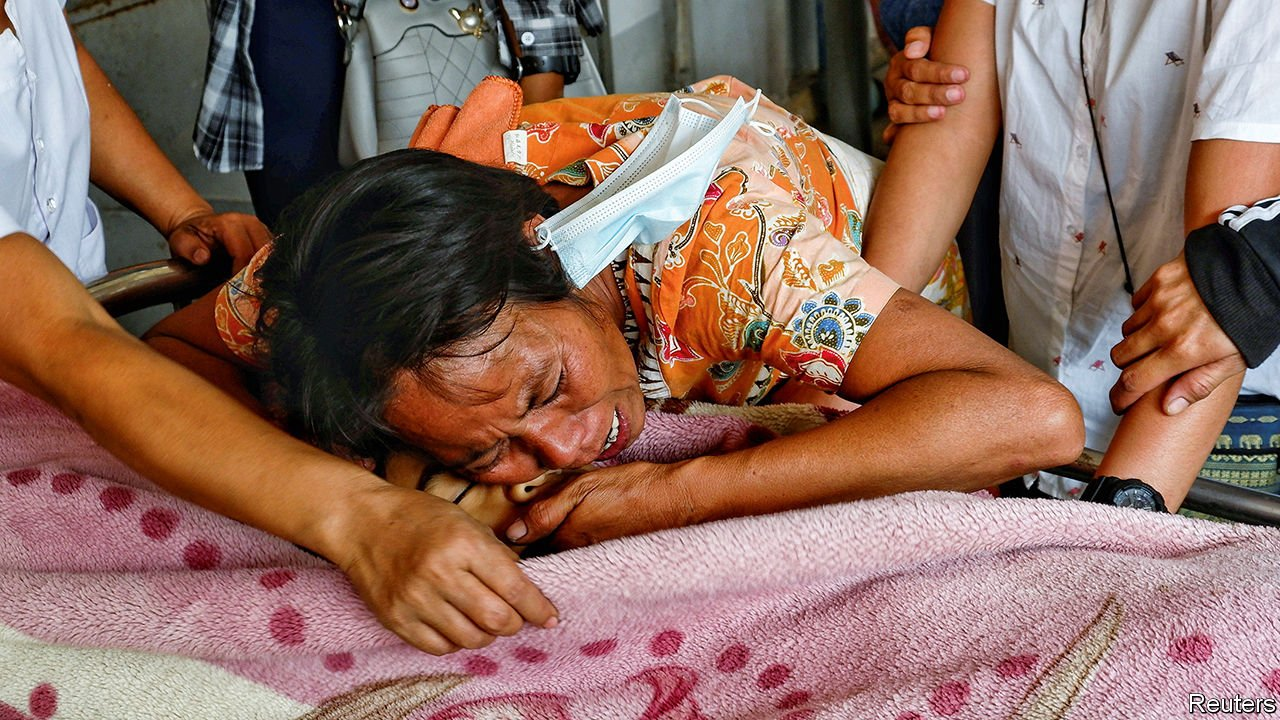
\includegraphics[width=0.8\textwidth]{images/20210327_WWP003_0.jpg}
\end{figure*}
\textbf{Myanmar's} army continued to shoot at demonstrators and rampage through neighbourhoods where there have been protests against the military coup. Among the victims was a seven-year-old girl, one of at least 260 people killed by the security forces since February 1st. Thousands have been arrested. A court hearing for Aung San Suu Kyi, Myanmar's deposed leader, had to be adjourned because of problems with the internet, which the army has shut down. 

\textbf{North Korea} fired two ballistic missiles off its east coast, a reminder to Joe Biden that the regime remains a threat to stability in East Asia. 

Two Canadians went on trial for \textbf{espionage} in China, in separate cases. Western diplomats believe their arrest two years ago was in response to the detention in Canada of an executive at Huawei. 

\href{/node/21799725}{\textbf{China} announced sanctions} against several Europeans, including members of the European Parliament and academics. Its action followed co-ordinated declarations by America, Britain, Canada and the EU of sanctions against four Chinese officials involved in the persecution of ethnic Uyghurs in the Chinese region of Xinjiang. 

The row over the \href{/europe/2021/03/25/europes-plans-to-restrict-vaccine-exports-endanger-itself-and-the-world}{export of}\textbf{covid-19 vaccines} deepened, as the European Commission in Brussels published proposals that would allow the EU to block the export of doses to countries that do not themselves export vaccines to Europe, or that already enjoy significantly higher inoculation rates than the EU does. 

\textbf{Germany's} chancellor, Angela Merkel, suffered an embarrassing defeat when she reversed a tightening of lockdown rules over Easter following objections from the leaders of many of Germany's 16 states. Infections are surging again in Germany and many other EU countries, leading to tougher restrictions in a number of them, including France. 

\textbf{Turkey's} president, Recep Tayyip Erdogan, fired his central-bank governor after he raised interest rates to tame inflation, as central-bank governors do. \href{/node/21799710}{Markets were spooked} by the sacking, and the lira sank. This is the third central-bank chief Mr Erdogan has dismissed in two years. 

\href{/node/21799714}{Nicola Sturgeon}, \textbf{Scotland's} first minister, survived a vote of no confidence. This came after a parliamentary inquiry concluded there were flaws in her government's handling of sexual-abuse allegations against her predecessor, Alex Salmond, though an independent inquiry cleared her of breaching the ministerial code. She still hopes to win big in an election in May. 

\href{/node/21799726}{\textbf{Israelis} voted} in a parliamentary election, the fourth in less than two years. Likud, the party of Binyamin Netanyahu, the prime minister, won the most seats. But his right-wing bloc looks to be short of a majority. The opposition, meanwhile, is fragmented. If neither side is able to form a government, Israel will probably hold a new election. 

\textbf{Saudi Arabia}\href{/node/21799727}{offered a ceasefire} to the Houthi rebels in \textbf{Yemen}. The kingdom has been fighting on behalf of the Yemeni government, which was dislodged by the Houthis in 2015. The Saudis offered to ease a blockade; the Houthis said this wasn't enough. 

Jihadists raided several villages in \textbf{Niger} near its border with Mali, killing at least 137 people. This year has seen a marked deterioration in security in the region. 

Denis Sassou Nguesso won re-election as \href{/middle-east-and-africa/2021/03/24/congo-brazzavilles-president-is-re-elected-after-his-rival-dies-of-covid-19}{president of \textbf{Congo-Brazzaville}}, which he has ruled for 36 years. Various countries, including France and America, have taken steps to confiscate his family's assets, alleging they were bought with embezzled funds. 

The state-funded Ethiopian Human Rights Commission accused Eritrean troops of killing more than 100 civilians in the \textbf{Ethiopian} city of Axum in November. Ethiopia's prime minister, Abiy Ahmed, has acknowledged that Eritrean troops crossed the border during Ethiopia's civil war against the northern region of Tigray. 

In New York a jury found Geovanny Fuentes Ramirez guilty of trafficking cocaine. During the trial Juan Orlando Hernández, the president of \textbf{Honduras}, was repeatedly mentioned in the proceedings. Mr Fuentes Ramirez claimed that he had bribed Mr Hernández and let him access millions of dollars-worth of the drug. Mr Hernández denies all allegations. 

Joe Biden put Kamala Harris in charge of co-ordinating efforts with Mexico, El Salvador, Guatemala and Honduras to reduce the flow of migrants attempting to cross the US \textbf{-Mexico border}. The vice-president's priority is to stop unaccompanied children being sent to America; around 11,000 were detained between February 28th and March 20th, up from 5,600 in January. 

\textbf{Virginia} abolished the death penalty, the first state in the American South to do so. It had executed more convicts than any other state, bar Texas. 

America's Supreme Court said it would look at reinstating the death sentence handed down to Dzhokhar Tsarnaev, the surviving bomber of the \textbf{Boston marathon} in 2013. Last year a federal appeals court found problems in the jury selection at Mr Tsarnaev's trial, and ordered a new hearing to determine his sentence. 

\begin{figure*}[h]
\centering
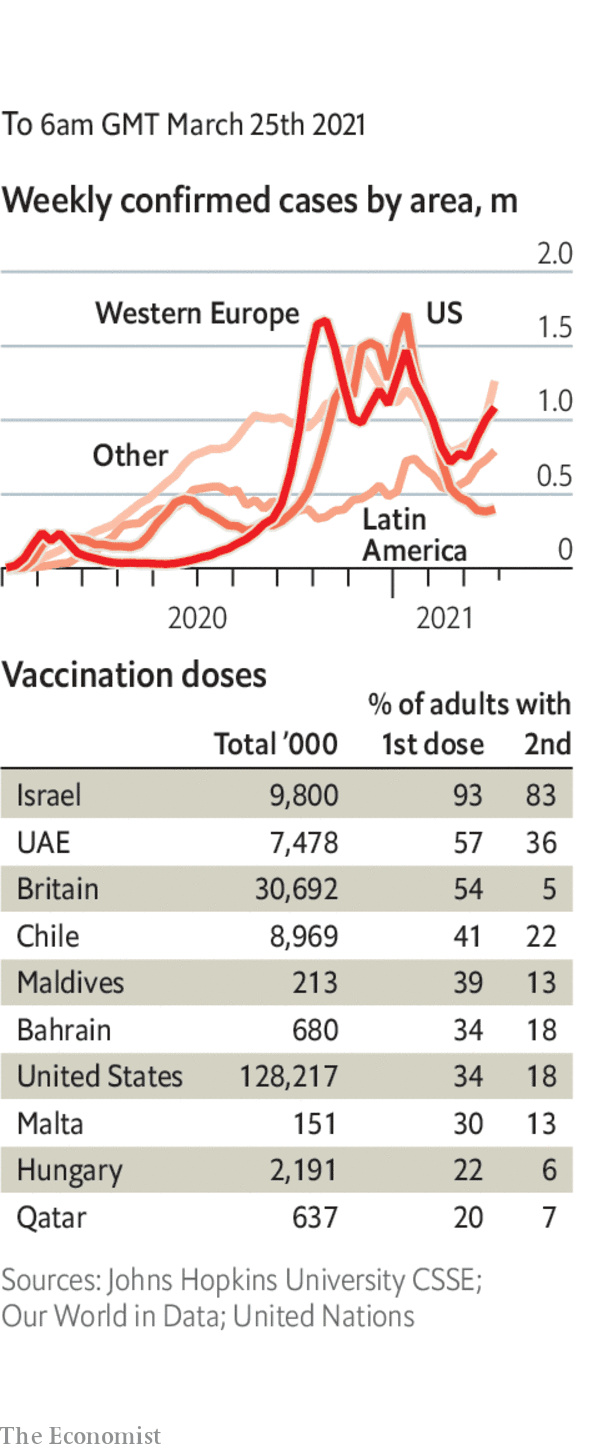
\includegraphics[width=0.4\textwidth]{images/20210327_WWC051.png}
\end{figure*}


Amid a surge in cases, the \textbf{Indian} government was urged to speed up its inoculation programme. Only 44m doses have been administered so far. \href{/asia/2021/03/27/india-and-china-are-finding-vaccine-diplomacy-tricky}{India has blocked exports of the AstraZeneca vaccine} so that they can be used domestically. 

Imran Khan, \textbf{Pakistan's} prime minister, tested positive for covid-19, apparently with only minor symptoms. 

Despite having the best vaccine programme in Latin America, \textbf{Chile} went back into quarantine. A rise in infections has possibly been caused by many people taking holidays in January and February, and excess confidence in the vaccine roll-out. 

In \textbf{Britain} the government said it was considering making it mandatory for care-home workers to get the jab. 

Spectators from overseas were banned from the \textbf{Tokyo Olympics}, which start in July. 
\clearpage
\subsubsection{ }
\subsection{Business this week }
\paragraph{Print Edition | The world this week  \quad \color{gray}{Mar 25th 2021 }}
\begin{figure*}[h]
\centering
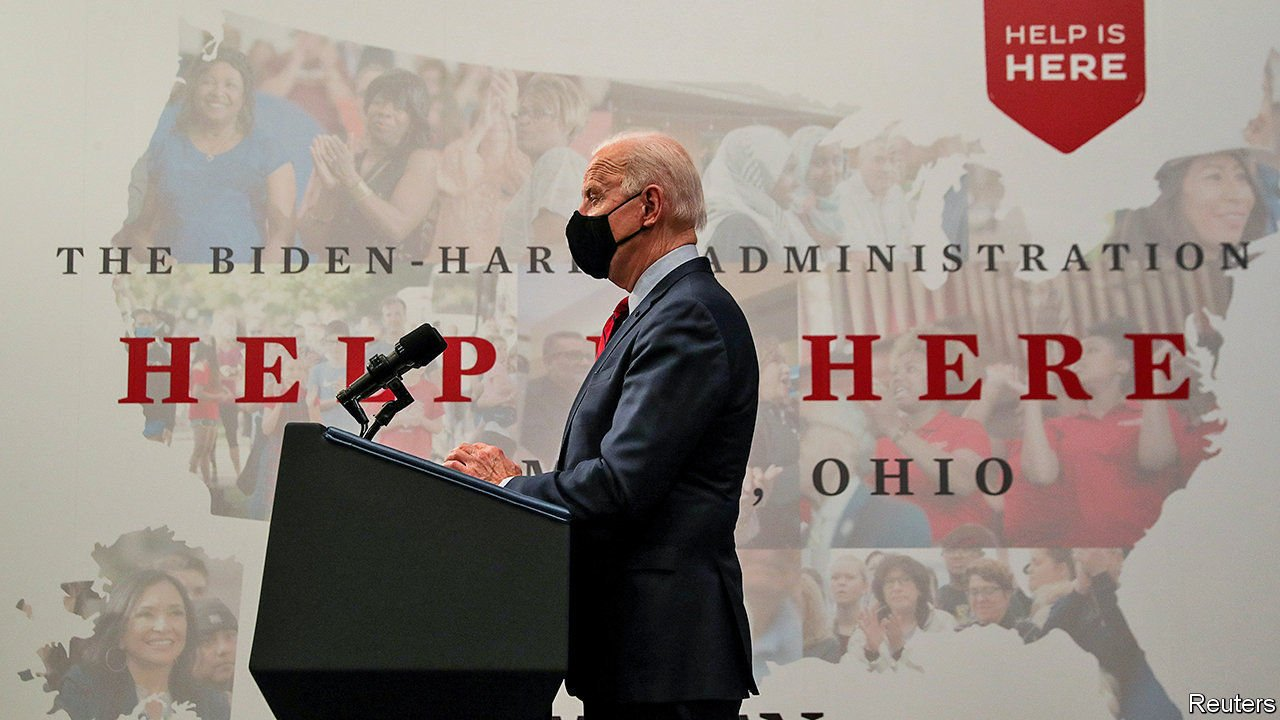
\includegraphics[width=0.8\textwidth]{images/20210327_wwp501.jpg}
\end{figure*}
Joe Biden is reportedly contemplating a \$3trn bill on infrastructure and education. The president has said his \href{/finance-and-economics/2021/03/25/just-how-anchored-are-americas-inflation-expectations}{\textbf{American Rescue Plan}} will be ambitious, but the size of the price tag, on top of the \$1.9trn stimulus package, has rekindled concerns about an overheating economy and inflation. Larry Summers, an economic guru in the Clinton and Obama administrations, warned Democrats and Republicans that they were being irresponsible, saying that America risks a ``dramatic fiscal-monetary collision''. 

\textbf{Deliveroo's} forthcoming IPO could see it valued at up to £8.8bn (\$12bn) based on the upper range at which it intends to price its shares. That would make it London's biggest stock debut since Glencore in 2011. Amazon holds 15.8\% of the food-delivery service, which will fall to 11.5\% after the IPO. 

\textbf{Baidu's} secondary listing of stock in Hong Kong was a damp squib. The tech giant follows other Chinese internet companies by listing in the city, though its shares barely rose on the first day of trading, and fell subsequently. 

\textbf{Canadian Pacific}, which operates freight rail along the Canadian border and the American Midwest, agreed to buy \textbf{Kansas City Southern} for \$29bn. The deal creates the first rail network linking Canada, Mexico and the United States. KCS transports goods in ten American states and in Mexico, where its network stretches to southern ports. America's freight-rail regulator must first give a green light to the merger. 

Pat Gelsinger, \textbf{Intel's} new boss, announced a turnaround plan for the world's biggest chipmaker, which has seen its share price sag. As well as making its own products, the company plans to produce more chips for other firms, a business model popularised by TSMC and Samsung. 

General Motors and Hyundai became the latest carmakers to announce production cuts as a result of a global \textbf{shortage of microchips}. Those shortages, triggered by the unpredictable effects of the pandemic, may get worse before they get better. A fire at a chip plant owned by Renesas Electronics, which supplies car firms, will halt production for a month. 

A container ship got itself wedged across the \href{/node/21799686}{\textbf{Suez canal}}, obstructing an important supply route for goods between Asia and Europe, and oil from the Middle East and Russia. Around 12\% of global trade passes through the canal. At 400 metres in length, the \emph{Ever Given} is one of the world's biggest ships. 

\href{/node/21799702}{\textbf{Saudi Aramco's} annual net profit fell} by almost half, to \$49bn, because of last year's plunge in demand and tumbling oil prices. The oil company still intends to pay a dividend, much of which will go to the Saudi government, its biggest shareholder. \textbf{Oil prices}, meanwhile, had another wobbly week on concerns that supplies would be disrupted by the blocked Suez canal. This follows the biggest weekly drop in prices since October. 

According to reports, the Securities and Exchange Commission has told ConocoPhillips and Occidental to allow their shareholders a vote on targets for \href{/node/21799741}{\textbf{cutting emissions} from products} used by their customers, rejecting claims that this amounts to micromanagement. Meanwhile a study by the Energy and Climate Intelligence Unit, a British organisation, warned that a lack of transparency about net zero-carbon objectives will lead to companies being accused of \textbf{greenwashing}. A fifth of the world's 2,000 biggest companies now have such goals. 

\textbf{Cineworld} said it would re-open some of its American picture houses in April, as states ease covid-19 restrictions. ``Godzilla vs Kong'' will be the first feature it shows. Underscoring how lockdowns have changed viewing habits, the world's second-biggest cinema chain has had to secure an agreement from Warner Brothers, the film's distributor, for movies to be screened in cinemas first before they are released on streaming services. 

A survey of chief executives by KPMG shone a light on \textbf{future work practices}. A quarter think the pandemic has changed their company for ever; 90\% intend to ask employees if they have been vaccinated; and cyber-security has emerged as their number one threat. But only 17\% now think they will reduce their company's physical space, down from 69\% in August. 

\textbf{Remote working} was said to be a factor behind complaints from junior bankers at Goldman Sachs about their 95-hour work week. Grizzled veterans grouched that there was nothing new about long hours. David Solomon, the bank's boss, said they should take Saturdays off. Capturing the zeitgeist, Jane Fraser, the new CEO of Citigroup, called for a ``reset'' between working from home and the office. In a move that would delight staff everywhere, she has instated Zoom-free Fridays. 
\clearpage
\subsubsection{ }
\subsection{KAL's cartoon }
\paragraph{Print Edition | The world this week  \quad \color{gray}{Mar 27th 2021 }}
\begin{figure*}[h]
\centering
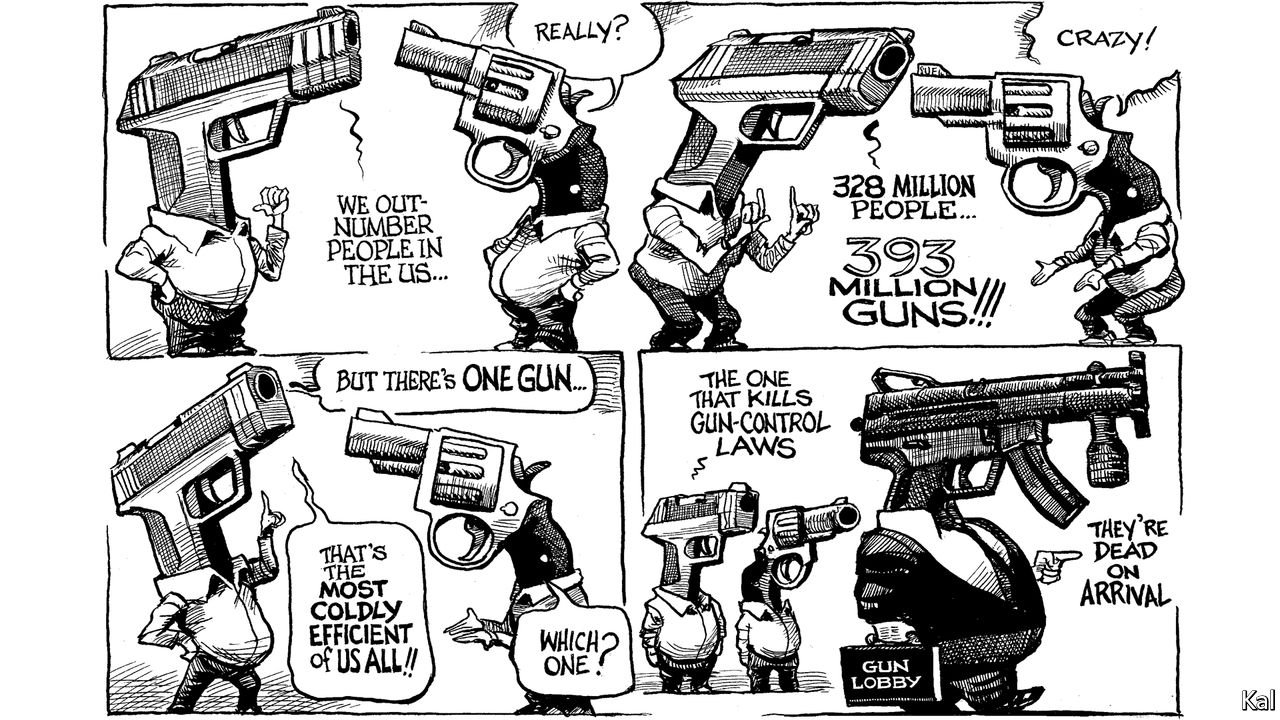
\includegraphics[width=0.8\textwidth]{images/20210327_wwd000.jpg}
\end{figure*}

\clearpage
\section{Leaders }
\subsubsection{Science after the pandemic }
\subsection{Bright side of the moonshots }
\paragraph{Print Edition | Leaders  \quad \color{gray}{Mar 27th 2021 }}
\begin{figure*}[h]
\centering
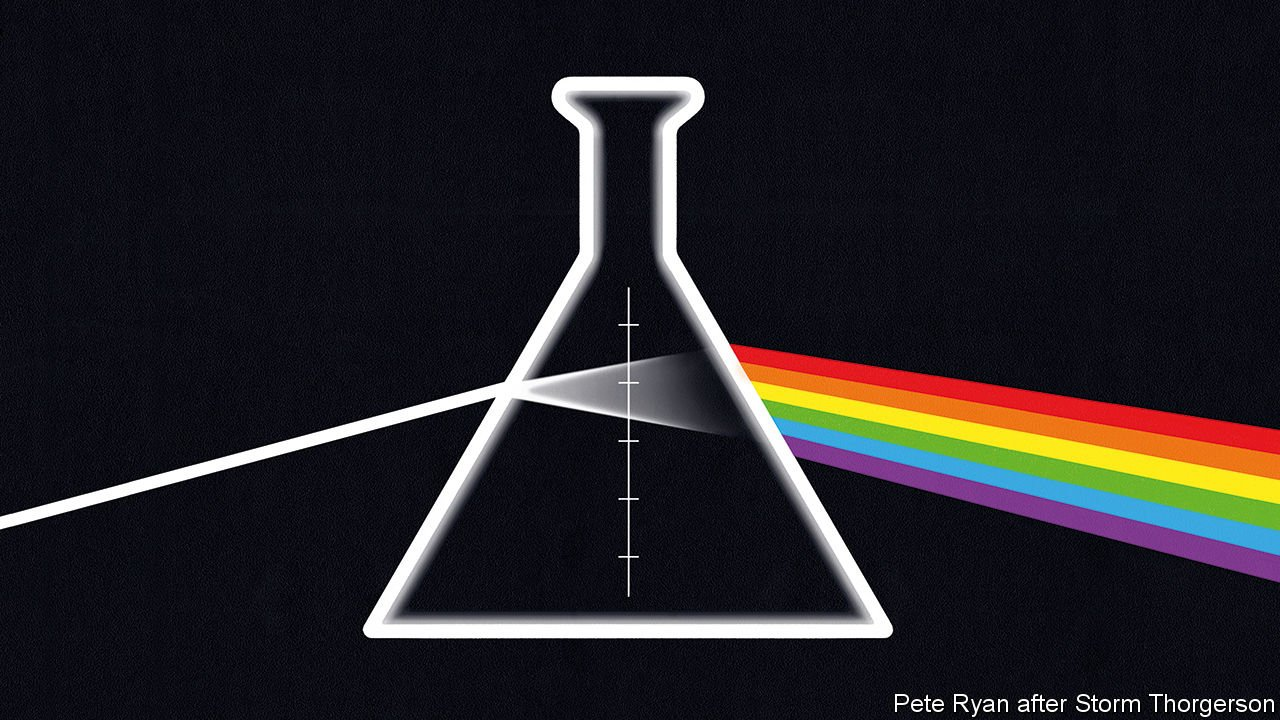
\includegraphics[width=0.8\textwidth]{images/20210327_LDD001_0.jpg}
\end{figure*}
\lettrine{T}HE FIRST virus to have its genome read was an obscure little creature called MS2; the 3,569 RNA letters it contained were published in 1976, the hard-won product of some ten years' work in a well-staffed Belgian laboratory. The SARS-CoV-2 genome, almost nine times longer, was published just weeks after doctors in Wuhan first became concerned about a new pneumonia. That feat has since been repeated with getting on for 1m different samples of SARS-CoV-2 in the hunt for \href{/the-americas/2021/03/27/brazils-mismanagement-of-covid-19-threatens-the-world}{fearsome variants} like the one ravaging Brazil. Within weeks of its publication, the original genome sequence became the basis for the \href{/europe/2021/03/25/europes-plans-to-restrict-vaccine-exports-endanger-itself-and-the-world}{vaccines} that today are stymieing the virus wherever supplies, politics and public confidence allow. 

It is hardly remarkable that medical science has moved on since 1976. But the covid-19 pandemic has brought the sharp joy of seeing decades of cumulative scientific progress in sudden, concerted action. The spate of data, experiments and insights has had profound effects on the pandemic---and, indeed, on the future of medicine. It is also an inspiration. Around the world, scientists have put aside their own work in order to do their bit against a common foe. Jealously guarded lab space has been devoted to the grunt work of processing tests. Covid-19 has led to some 350,000 bits of research, many of them on preprint servers that make findings available almost instantaneously. 

The basis of all this is the application of genetics to medicine in a systematic and transformative way---not just in understanding the pathology of diseases but in tracking their spread and curing and preventing them. This approach could underpin what is becoming known as ``natural security''---the task of making societies resilient in the face of risks stemming from their connection to the living world, whether because of disease, food insecurity, biological warfare or environmental degradation. 

 

The application of genetics to medicine partly reflects huge, rapid gains in efficiency. Reading the DNA in a human genome cost \$10m in 2007, today it takes less than \$1,000 and a fraction of the time. Coupled with ever-better ways of \href{/technology-quarterly/2021-03-27}{synthesising and editing genes}, this has enabled cleverness little short of the miraculous. Before the pandemic, these trailblazing techniques were not much talked about beyond the laboratory. Having shown their mettle against a brand new disease, they have burst out into the open. 

Take the vaccination technology rapidly developed by Moderna of America and BioNTech of Germany, building on years of patient and often unsung work on RNA, a store of genetic information. It is remarkable that you can simply instruct the body's cells to make the viral protein you have designed to prime the immune system. The RNA vaccines are testament to the insight of Eddie Cantor, a comedian, that it takes 20 years to become an overnight success. 

With this proof of concept, the investments of companies that have worked hard on RNA may now pay off. To some extent, \href{/briefing/2021/03/27/covid-19-vaccines-have-alerted-the-world-to-the-power-of-rna-therapies}{RNA medicine} divorces form from function. An RNA vaccine against any disease is a message written in genetic code: a vaccine against malaria, or some form of cancer, can be made in the same way and with the same equipment as a SARS-CoV-2 vaccine. If this provides a platform for getting cells to do all sorts of specific things and to desist from others, as it promises to, medicine will become both more powerful and more personal. Therapies tailored to rare, even one-off, genetic abnormalities should become routine. 

The pandemic has also demonstrated the value of gene-sequencing technologies. Observing SARS-CoV-2 as it mutates is essential if the world is to understand and defend itself against dangerous variants. Should covid-19 become endemic, as is likely, sequencing will become the basis for developing regular booster shots. More broadly, routine sequencing is one of the best ways of knowing what is out there. Companies have done brilliantly in producing powerful sequencing systems for trained technicians. Now the world needs cheap, ubiquitous and reliable systems that can be used in the prison sick bay or the rural health centre, on the farm or at the town sewage works, to act as early-warning systems for the spread of pathogens. 

Another area of work is where the pandemic has revealed a gap. Even today's progress has yet to produce small-molecule antivirals to combat SARS-CoV-2. A focus for natural security should be drugs aimed at the viral families most likely to cause trouble in the future. This is not something that the market will support on its own. New mechanisms that involve governments will be needed, such as funds for R\&D and trials and to buy stockpiles of medicine. Similar approaches should also be used for the looming threat of antibiotic-resistant bacteria. 

These innovations will have big consequences. General-purpose RNA medicine asks new things of firms and regulators---as do other platforms, including some forms of gene therapy. Regulators will need to take advantage of the fact that, say, a malaria vaccine and a SARS-CoV-2 vaccine are both made on the same platform by streamlining approval for them, while continuing to ensure safety. 

Drugs firms will have to adapt, as some chronic conditions may, in effect, be cured. Many are used to concentrating on the long-lasting afflictions that most trouble the rich world: heart disease, cancer, metabolic disorders, neurodegenerative conditions and the like. If drug development is more targeted on instructing cells what to do, rather than finding novel molecules against specific proteins, some of the know-how on which old-style pharma is based will be less relevant. Firms will need new pricing models and a new focus to their research. 

Technology will not, in itself, thwart pandemics. That goal also requires systems and institutions which use technology broadly and wisely. Without good systems, great technology will often provide only mediocre results, as it has in many covid-19 test-and-trace programmes. But the pandemic has shown that biomedical science has the tools and the enthusiasm to improve the world. The world must now build on both. {} 

\textbf{Dig deeper} 

\emph{All our stories relating to the pandemic and the vaccines can be found on our \href{/news/2020/03/11/the-economists-coverage-of-the-coronavirus}{coronavirus hub}. You can also listen to \href{/podcasts/the-jab-a-new-podcast-from-the-economist}{The Jab}, our new podcast on the race between injections and infections, and find trackers showing \href{https://www.economist.com/graphic-detail/tracking-coronavirus-across-the-world}{the global roll-out of vaccines}, \href{https://www.economist.com/graphic-detail/coronavirus-excess-deaths-tracker}{excess deaths by country} and the virus's spread across \href{https://www.economist.com/graphic-detail/tracking-coronavirus-across-europe}{Europe} and \href{https://www.economist.com/graphic-detail/tracking-coronavirus-across-america}{America}.} 
\clearpage
\subsubsection{Turkey and emerging markets }
\subsection{Turkey's economic woes should be a warning for other countries }
\paragraph{Print Edition | Leaders  \quad \color{gray}{Mar 25th 2021 }}
\begin{figure*}[h]
\centering
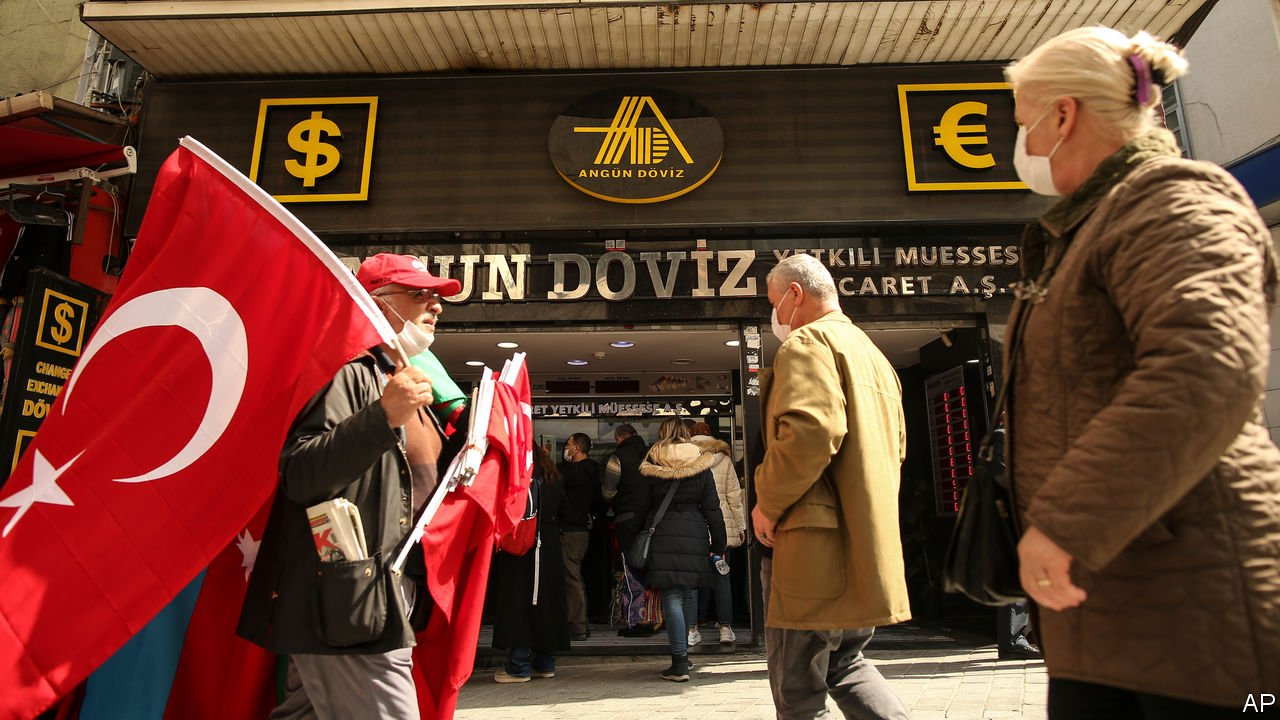
\includegraphics[width=0.8\textwidth]{images/20210327_ldp501.jpg}
\end{figure*}
\lettrine{I}STANBUL'S STOCK exchange does not open until shortly before 10am, a more civilised hour than most bourses. Investors therefore had time to brace themselves on March 22nd before discovering the full cost of President Recep Tayyip Erdogan's reckless decision to fire Turkey's admired central-bank governor, Naci Agbal, over the preceding weekend. The selling frenzy triggered an automatic suspension of trading twice in the first 45 minutes. Combined with a deep fall in the lira, Turkey's stocks declined by over 16\% in dollar terms by the end of the day. 

Turkey has grown faster than most emerging markets over the past decade, and even managed to eke out a modest expansion last year. But as Mr Erdogan's party has accumulated power and audacity, it has eroded the institutional constraints that once ensured economic stability, including the autonomy of the central bank. Mr Agbal was unceremoniously sacked for doing too much to stop inflation. His predecessor was fired for failing to steady the lira. Mr Erdogan has yet to grasp that a central bank cannot avoid one of these improprieties without committing the other. He has now \href{/europe/2021/03/25/a-debacle-at-turkeys-central-bank}{removed three central-bank governors} in two years. 

Mr Erdogan's macroeconomic muddles and meddling reflect both his own intellectual confusion and the inconsistent demands of his supporters. Turkey's construction industry, which ensures growth and jobs, thrives on easy credit. That contributes to inflation and a flight from the lira. But Turks, especially merchants and small-business folk, who keep much of their money in dollars or euros, vehemently oppose exchange controls. The result is an unstable currency and unstable prices. Turkey is trying to emulate China's growth strategy (featuring state-backed credit for property and infrastructure investment) without the benefit of its docile depositors and trapped savings. 

\begin{figure*}[h]
\centering
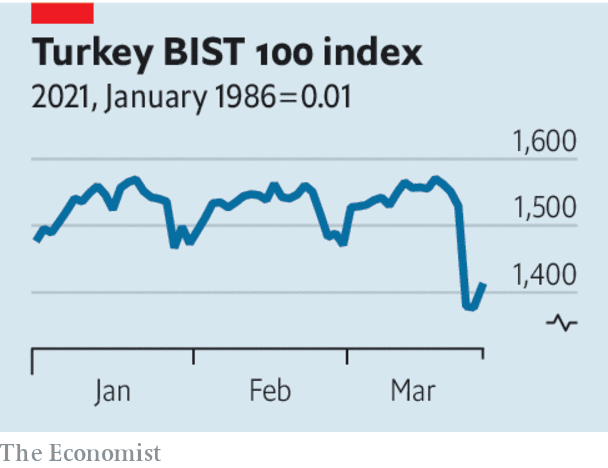
\includegraphics[width=0.4\textwidth]{images/20210327_LDC001.png}
\end{figure*}


Such considerations are the burden Turkey alone must bear. But the country's problems also reflect broader concerns that weigh on emerging markets in general. The interest-rate rise that cost Mr Agbal his job was partly a response to a common threat. As the world economy revives, commodity prices recover and American bond yields rise, so \href{/finance-and-economics/2021/03/25/trade-inflows-in-asia-fuel-debate-over-currency-intervention}{emerging markets} could start to face a squeeze. Inflation will move mechanically higher as the depressed prices of last year give way to a more normal pattern this year. If that rise in prices raises expectations of sustained future inflation, central banks will have to respond, as Brazil's central bank did last week when it raised interest rates more than expected. If they do not, inflation will begin to feed on itself. 

Fortunately, the holders of emerging-market assets can take some comfort. In most other big markets central banks have larger amounts of hard-won credibility to draw on. Russia's respected monetary-policy chief has been in her job for almost eight years. Brazil has just passed a law that formalises the central bank's independence. The average inflation rate among the 27 members of MSCI's benchmark emerging-market equity index is only about 4\%, compared with over 15\% in Turkey. Indeed, in countries like Thailand and Malaysia, prices are still falling. Partly because the lira cannot hold its value, Turkey is also unusually reliant on borrowing in other people's currencies. The combined foreign-currency debts of its government, banks and companies amounted to over 80\% of GDP at the end of 2020. In Brazil the figure was only half that. 

For all these reasons, other emerging markets should be able to withstand any temporary fallout from the fuss in Turkey. Nevertheless, they should heed the country's cautionary tale: if you rely on foreign capital it is risky to compromise central bank independence, especially when global interest rates are rising. Emerging-market investors will treat Turkey as an unfortunate exception only for as long as emerging-market policymakers learn from its unfortunate example. {} 
\clearpage
\subsubsection{Digital commerce }
\subsection{Fintech comes to America at last }
\paragraph{Print Edition | Leaders  \quad \color{gray}{Mar 27th 2021 }}
\begin{figure*}[h]
\centering

\includegraphics[width=0.8\textwidth]{images/20210327_ldp502.jpg}
\end{figure*}
\lettrine{A}MERICA IS HOME to both Silicon Valley and Wall Street, yet it has long seemed in the dark ages on digital payments. Until 2018 card purchases required hand signatures, 15 years after Europe switched to chip-and-pin. A cosy credit-card duopoly, consisting of Visa and Mastercard, works with the banks to issue cards, with the result that there has been too little competition and sky-high profit margins. Asia has leapt ahead, with pervasive, fast and dirt-cheap payments services, and a new generation of dynamic fintech firms that have rapidly reached scale. Having outdated and expensive digital financial plumbing is no mere technicality: as online shopping becomes a bigger part of everyday spending, it threatens to become a heavy tax on innovation. And it means too few people, especially in poorer households, have access to cheap and simple financial tools. 

The good news is that the picture in America is changing for the better. Thanks to the pandemic, there has been a surge in payments online and experimentation by consumers with new services provided by digital-payments firms. In the past quarter the volume of transactions on PayPal was 36\% higher than a year earlier. The number of people using Square's digital Cash App rose by 50\% to 36m during 2020. Investors are now betting that these two firms, together with Stripe and Adyen (which is Dutch), form a quartet that can take on America's stodgy financial establishment. (The chairman of \emph{The Economist}'s parent group is a director of Square.) PayPal is worth \$275bn, nearing Bank of America, the country's second-biggest lender. 

Yet there is a catch. Despite the rise of innovative firms, fees for American consumers have yet to fall by much. Square charges 2.6\% on the average transaction; Stripe's fee nears 3\%. By contrast, China's big fintech firms charge below 0.5\%. Fees have been kept low by a fierce price war. 

A big part of the problem in America is that, rather than route purchases through competing payment pipes, the fintechs still often have little choice but to rely on America's credit-card networks to connect merchants, banks and consumers. The credit-card firms continue to demand a high rent of roughly 2\%. Funds can take days to travel. That reflects the power and entrenched position of Visa and Mastercard. They process 86\% of card payments through huge networks linking most shops and firms, which have to sign up to detailed terms and conditions. 

You might think that the answer is antitrust action against the credit-card firms. America's competition watchdogs are growling. Last November the Department of Justice sued to block Visa's \$5.3bn purchase of Plaid after Visa's boss described it as an ``insurance policy'' to neutralise a ``threat to our important US debit business''. The two firms abandoned the deal. On March 19th the \emph{Wall Street Journal} reported that the justice department had started a new probe over whether Visa is inhibiting merchants from switching to cheaper services. But do not get your hopes up. The courts, which decide most antitrust cases in America, take ages to act and tend to be too lenient. A big antitrust case against American Express in 2017 flopped. 

Instead, the key to making payments more competitive in America is to create a new network of financial plumbing: a ``real-time'' interbank-payment system allowing for near-instant and cheap transfers. Swathes of Europe and Asia have already done this. Once this exists, banks and fintechs can build products, standards and services on top of it. In Singapore and the Netherlands, for example, those efficient payment pipes are open to digital wallets, which can process payments in a few clicks, taps or by scanning a QR code. 

America's own effort at instant payments, backed by the Federal Reserve and known as FedNow, is to launch in 2023. The big banks and credit-card firms are keen to delay a system that could disrupt the status quo. The government and the Fed should not just ignore their grumbles but bring forward the timetable. The pandemic has shown that online transactions have come of age. It has also shown that the public sector can act quickly and effectively when it has to. Cheap and swift digital payments are a prize that should be viewed as a priority. {} 
\clearpage
\subsubsection{Mid-life crisis }
\subsection{Bangladesh's growth has been remarkable, but is now at risk }
\paragraph{Print Edition | Leaders  \quad \color{gray}{Mar 25th 2021 }}
\begin{figure*}[h]
\centering

\includegraphics[width=0.8\textwidth]{images/20210327_LDP001_0.jpg}
\end{figure*}
\lettrine{``W}ON'T YOU give some bread to get the starving fed? We've got to relieve Bangladesh,'' sang George Harrison, a former Beatle, in 1971. His pleading was warranted. No sooner had local politicians declared the independence of the eastern half of Pakistan (as Bangladesh had previously been) on March 26th of that year than the Pakistani army initiated a brutal war to crush the separatists, at a cost of somewhere between 500,000 and 3m lives. The fighting, along with devastating floods and cyclones, had turned the new country into one of the most destitute spots on Earth. 

Fifty years on, the improvement in the lives of ordinary Bangladeshis has been remarkable. In 1972 GDP per person was almost 40\% lower in \href{/node/21799723}{Bangladesh} than in Paki-stan. Now it is more than 40\% higher. The economy was growing by around 8\% a year before the pandemic struck---the fastest pace in Asia. The country's proliferating garment factories provide a decent livelihood for millions. By the World Bank's reckoning, Bangladesh has graduated from ``least developed'' to ``developing'' or ``lower middle-income''---a huge advance on the wasteland of 1971. 

By other measures, Bangladesh is doing even better. Infant mortality, which used to be higher than in both Pakistan and India, is now lower. A typical Bangladeshi lives three years longer than the average Indian, and five years longer than the average Pakistani. Bangladeshi women, in particular, have seen their circumstances improve dramatically: they are more likely to have gone to school, to be able to read and to have a job than their counterparts in India and Pakistan. They also have fewer children---although with 170m people, Bangladesh is nonetheless the eighth-most-populous country in the world. 

This remarkable turnaround is not thanks to administrative stability or far-sighted leadership. On the contrary, since Bangladesh's birth its politics have been violent and tumultuous, marred by thuggish parties, frequent coups and extreme polarisation. The current prime minister, Sheikh Hasina Wazed (pictured), has been in office since 2009 and centralised power, eroded all checks on her authority and systematically undermined or co-opted independent institutions that might serve as rival sources of prestige. 

However, despite the constant political upheaval, two things have stood Bangladesh in good stead. The first is the moderation and practicality of ordinary Bangladeshis. Cultural conservatism in both India and Pakistan has impeded women from working outside the home. But in Bangladesh the share of women in the workforce has risen steadily, from 3\% in 1974 to 36\% in 2019. It is these women who staff the garment factories, and so have enabled the rapid economic growth of recent years. 

The second factor behind Bangladesh's good fortune has been the openness of successive governments to outside assistance. This stance was born of necessity: the war of independence left the country, including all levels of administration, in such tatters that there was little alternative but to take whatever help was on offer, be it from returning expats, aid agencies or former Beatles. The energy and creativity of the many charities and NGOs, in turn, helped propel rapid improvements in the health and welfare of ordinary Bangladeshis long after the immediate damage of the war had been repaired. Microcredit---helping the poor improve their lot by giving them tiny loans, even though commercial banks would not have considered them creditworthy---was pioneered in Bangladesh. NGOs have also worked closely with the government on everything from insulating farmers from the consequences of bad harvests to distributing contraceptives. 

Sheikh Hasina, daughter of the hero of independence, Sheikh Mujibur Rahman, is making much of the country's 50th birthday. Yet her increasingly authoritarian ways are damaging the very traits that have made it so successful. Big NGOs have been brought to heel. After Muhammad Yunus, who won the Nobel peace prize for his work on microfinance, mused about starting a political party, he found himself ejected from Grameen Bank, the biggest provider of small loans to the needy. By the same token, to court devout voters Sheikh Hasina has allied with doctrinaire Muslim groups, which have agitated against secularism, women's rights and sexual freedoms. A group of such radicals, along with members of the ruling party's youth wing, recently ransacked a Hindu village after an inhabitant criticised their leader on Facebook. 

The record of the past 50 years provides an enormous amount to celebrate. But Sheikh Hasina does not seem to understand the legacy she has inherited. Bangladesh has not come so far thanks to a strong, intolerant, centralised government, but rather for the lack of one. {} 
\clearpage
\subsubsection{Knocked out and locked up }
\subsection{A huge share of prisoners have brain injuries. They need more help }
\paragraph{Print Edition | Leaders  \quad \color{gray}{Mar 27th 2021 }}
\begin{figure*}[h]
\centering

\includegraphics[width=0.8\textwidth]{images/20210327_LDP002_0.jpg}
\end{figure*}
\lettrine{A} KNOCK ON the head can change the course of a whole life. \href{/international/2021/03/27/brain-injuries-are-startlingly-common-among-those-who-have-committed-crimes}{Traumatic brain injuries} affect around one in ten people in rich countries. Those who have experienced such injuries are more likely to suffer mental-health problems and loneliness. They are more likely to struggle with addiction to drink or drugs, or to be homeless. They are also more likely to commit crimes, including violent ones, although most do not. Estimates vary, but they consistently show that people in prison are many times more likely to have brain injuries. 

Those whose brains are not ``neurotypical'' in other ways also make up an extraordinarily large share of the prison population. People with learning difficulties, intellectual disabilities and autism are all over-represented behind bars. In Canada young people with fetal alcohol spectrum disorder, which is the result of exposure to alcohol in the womb and which damages the brain's frontal lobe, are incarcerated at 19 times the rate of the wider population. 

A traumatic brain injury is caused by a blow to the head powerful enough to disrupt brain function. The most common causes are falls, fights, assaults and car accidents. The people most prone to suffering them are young men, especially poor ones. A child from a poor background is four times more likely to suffer a brain injury before the age of five than a child from a wealthy background. Even mild concussion can cause long-term damage. Brain injuries can impair the way people think, experience emotions and control their own behaviour. Problems often occur when there is damage to the prefrontal cortex, which is associated with aggression and a lack of inhibition. 

Preventing brain injuries would avert much suffering, both directly (by reducing the number of people so impaired) and indirectly (by reducing the number who hurt others). Education is a good place to start. Parents and children need to be taught about the risks, urged to wear bicycle helmets and deterred from drunk-driving. Schools and police should do more to curb violence---by far the main cause of traumatic brain injuries affecting women in prison is domestic abuse. Prevention policies would pay for themselves, because brain injuries are expensive. In Britain the average lifetime cost of one in a 15-year-old who goes on to offend is estimated to be around £345,000 (\$475,000). 

Not all injuries can be averted, of course. So more help is needed for those who suffer them. Most important such injuries need to be identified earlier, especially in children, and teenagers. Hospitals need to try harder to spot and report brain trauma in children who show up with other injuries, and to ensure that they receive follow-up care. In the most neglected schoolchildren, screening might catch injuries. Once identified, they can be treated---sometimes with medication (such as stimulants for cognitive functioning and fatigue), most often with neuro-rehabilitation. Physical, speech and occupational therapies can help people to regain lost functions, learn new skills and overcome difficulties with attention and impulse control. Psychological support can help them control their emotions. 

And those who end up in prison need help turning their lives around. From April, British prisons will have to screen all inmates who have experienced domestic violence for brain injuries. Such screening should be extended to all prisoners. It would enable staff to identify those whose brains have been damaged and offer them appropriate support. Those with the most severe brain injuries should probably not be in prison at all. Mental-health courts in parts of America have done a good job of diverting prisoners away from jail and into places where their mental-health problems can be treated. For many such people, neuro-rehabilitation centres would be cheaper than prison and better at reducing recidivism. 

Acknowledging the link between brain injuries and criminal behaviour is not to excuse lawbreaking. Most people with such injuries are capable of taking responsibility for their actions. However, it is easier to curb crime if you understand the factors that make it more likely, of which neurodisabilities are an important and neglected one. More research is needed, but it is striking that offenders with attention-deficit hyperactivity disorder who take their medication are a third less likely to reoffend than those who do not. Punishing people without also offering them the help they need is short-sighted and wrong. {} 
\clearpage
\section{Letters }
\subsubsection{On nuclear power, Namibia, Uber, jury trials, beer, Bob Dylan }
\subsection{Letters to the editor }
\paragraph{Print Edition | Letters  \quad \color{gray}{Mar 27th 2021 }}
\begin{figure*}[h]
\centering
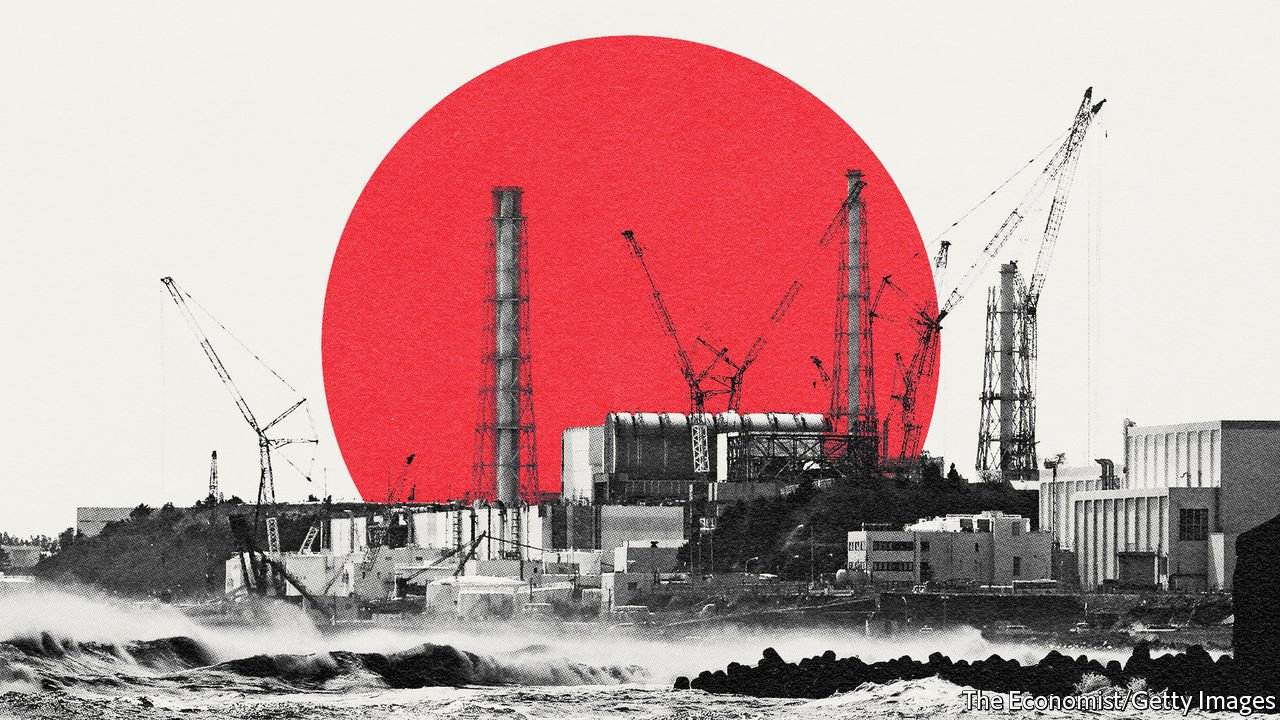
\includegraphics[width=0.8\textwidth]{images/20210306_ldd002.jpg}
\end{figure*}
{{{{Letters are welcome via e-mail to }\href{/cdn-cgi/l/email-protection\#81ede4f5f5e4f3f2c1e4e2eeefeeece8f2f5afe2eeec}{{{[}email~protected{]}}}}}} 

Coverage of the Fukushima disaster tends to muddle two key facts (``\href{/leaders/2021/03/06/nuclear-power-must-be-well-regulated-not-ditched}{The lessons of Fukushima}'', March 6th). The first is that Fukushima has the lowest seawall elevation of all the Pacific-facing nuclear-reactor sites in Japan, making it significantly more susceptible to the risk from a tsunami. A higher location with backup power and cooling systems would have avoided the disaster. Despite misgivings about its low-lying position, the selection of the site was driven by politics. Securing approval from local constituencies is an incontestable requirement for nuclear operations in Japan over other considerations. 

The second key factor is design. All the Pacific reactors on that afternoon of March 11th 2011, including Fukushima, safely initiated emergency shutdown sequences in response to the earthquake, testimony to the Japanese nuclear industry's strong safety record. 

It was not the earthquake that caused the disaster, but a freak tsunami, combined with the Japanese nuclear industry's and population's inability to debate risk. Nuclear revival can be safe even in earthquake-prone Japan, and is essential if the country is to achieve carbon-neutral power. 

TROY FOWLER\\ Nuclear fuel team\\ Japan ``Sogo-Shosha'' General Trading Company, 2010-14\\ \emph{West Linn, Oregon} 

The new generation of advanced modular reactors being developed in Japan, America and Canada address all the issues you raised. Japan, for example, has a High Temperature Gas-cooled Reactor that is inherently safe, is 45\% more efficient than a pressurised water reactor and can be factory built in three to four years, rather than up to 15 years. It complements intermittent renewables as part of any reliable energy portfolio. 

The HTGR also produces 75\% less waste than current reactors. As some of the new advanced reactors can re-utilise spent fuel, Britain's legacy waste becomes an asset with intrinsic value, and no longer a liability. And how much better to deal with it under the watchful eye of Britain's regulator. 

IAN FELLS\\ Professor emeritus\\ Newcastle University 

A ``high level of regulation'' is only one necessary condition for attaining, as you contend, a ``very small'' risk of failure. In order to make nuclear power safer we must pay equal attention to nurturing a strong safety culture among our nuclear-power utilities. A safety culture is analogous to the human body's immune system that protects it against pathogens and fends off diseases. A safety culture based on trust, transparency and accountability is the key to the secure operation of nuclear reactors; it should also be the basis of relations and interactions among reactor suppliers, operators and regulators. 

PROFESSOR NAJMEDIN MESHKATI\\ Department of Civil and Environmental Engineering\\ University of Southern California\\ \emph{Los Angeles} 

Nuclear power has had its day. It is now prohibitively expensive to construct. Britain's Hinkley Point C reactor was granted a licence in 2012 and is not expected to be operating until 2026. It will have cost £23bn (\$32bn). As for small modular reactors, the proposed NuScale reactor in America is scheduled for 2029. 

PETER NASH\\ \emph{Sydney} 

The American government has not been able to prove that buried nuclear waste will be dealt with effectively. Yucca Mountain in Nevada was selected as the least unsatisfactory location only because Nevada has a small population and large remote areas. 

DAVID CALVIN GOGERTY\\ \emph{Idyllwild, California} 

There are other candidates to compete with Hitler as ``the worst racist in history'' (``\href{/britain/2021/03/04/a-chronicle-of-the-british-establishments-flirtation-with-hitler}{Nazi parties}'', March 6th). ``The Kaiser's Holocaust'' by David Olusoga and Casper Erichsen illuminates a chapter of the past not many of us learn about: the genocide of the Herero and Nama peoples of Namibia. Their slaughter served as a blueprint for the Nazis in many ways. General Lothar von Trotha's name may not be well known outside Germany and Namibia, but he is on a par with Hitler. 

SARA WAUGH\\ \emph{Lopez Island, Washington} 

Uber may have accepted the Supreme Court's ruling in Britain to treat its drivers like employees (``\href{/britain/2021/03/18/ubers-workers-benefit-from-a-supreme-court-decision}{Move fast and fix things}'', March 20th). But it will only pay the minimum wage once a driver accepts a booking. The drivers have claimed that up to half their time is spent waiting for rides, and this should rightly be considered part of their working hours. Would it be correct to pay supermarket workers only when they are scanning items? 

THOMAS PAPPAS\\ \emph{London} 

You suggested that the decision to host the trial of Andrea Sahouri, a journalist, at Drake University Law School was bizarre (``\href{/united-states/2021/03/13/press-freedom-under-pressure}{Press freedom under pressure}'', March 13th). On the contrary, selecting the case for our annual trial practicum was an invaluable learning experience for our students, and also helped shine an international spotlight on this prosecution. 

Remarkably, the vast majority of American law students can graduate without having ever seen a trial, let alone participated in one. That does not happen at Drake Law; we suspend regular classes for a week so that first-year law students can observe a real trial from the selection of the jury through to the verdict. Students have the opportunity to discuss tactical decisions and rulings with the attorneys and judges, and in most years, after the jury has reached its verdict, they are able to talk to jurors about their views of the evidence. 

The real-life nature of the case makes it a much more meaningful experience than the typical law-school simulation. Seeing a defendant led off in handcuffs at the end of a murder trial, as students witnessed several years ago, is something they will never forget, bringing home the dramatic power of the legal system over people's lives and liberty. 

JERRY ANDERSON\\ Professor of law\\ Drake University Law School\\ \emph{Des Moines, Iowa} 

One of the greatest opportunities presented by Britain's separation from the EU (``\href{/leaders/2021/03/13/how-britain-can-benefit-from-brexit}{Growing apart}'', March 13th) is differentiated excise duty. Allowing British pubs to enjoy a lower level of tax on draft beer, for example, was illegal under EU rules. Lowering the tax would provide a boost to a much-loved industry. 

PAUL WELLS\\ \emph{Sandy, Bedfordshire} 

``\href{/briefing/2021/03/06/covid-19-has-transformed-the-welfare-state-which-changes-will-endure}{Shelter from the storm}'' (March 6th) outlined welfare initiatives to beat the idiot wind. The pandemic has left us tangled up in blue and was no simple twist of fate. We're together through life but mourn fallen angels. And yes, we desire another side, more freewheelin'. I just got my first AstraZeneca shot of love, leaving me knocked out loaded. Oh mercy. A new morning. 

DREW FAGAN\\ \emph{Toronto} 
\clearpage
\section{Briefing }
\subsubsection{The medicine is the message }
\subsection{Covid-19 vaccines have alerted the world to the power of RNA therapies }
\paragraph{Print Edition | Briefing  \quad \color{gray}{Mar 27th 2021 }}
\begin{figure*}[h]
\centering

\includegraphics[width=0.8\textwidth]{images/20210327_FBD001_0.jpg}
\end{figure*}
\lettrine{M}OLECULAR BIOLOGY is not a popularity contest. But if it were, it would be a partisan one. The evolutionary biologists would pledge their allegiance en masse to DNA. The sequences contained in its regular coils knit together the stories of almost all life on the planet. Pharmacologists, being of a more practical bent, would instead vote for proteins. Proteins are not about sequence, but about shape; their complex, irregular outlines, and the ways that they can change, allow them to do almost all of the biological work that gets done in cells. And it is thanks to the way that particular drug molecules fit into those shapes that almost all drugs have their effects. 

There would be only a small following for ribonucleic acid (RNA), widely seen as a helpmeet molecule. It could be argued that the production of RNA is DNA's main purpose; it is certainly true that the production of proteins would be nowhere without it. But it is a backstage operator, not a star; hewing wood and drawing water, hard working but hardly glamorous, appreciated only by devotees. 

Or at least that was the case until vaccines made of RNA started giving protection against covid-19 to millions of people around the world every day. Now Cinderella has gone to the ball. Not only are RNA vaccines being considered for all sorts of other diseases, some of which have yielded to no other approach; other pharmaceutical uses of RNA look set to come into their own, as well. The way molecular biology is applied to medicine seems to be in the throes of revolution. 

The great unifying truth of molecular biology, uncovered during the intellectual revolution which followed the discovery of DNA's double-helix structure, is the way in which the worlds of shape and sequence are linked. The shape of a protein depends on the intricate way in which the chain of amino acids of which it consists is folded up. That depends in turn on the order in which amino acids of different types are strung together on that chain. And the order of the amino acids is a crucial part of the genetic information stored in the DNA sequences of the cell's genome. 

The transfer of information from the staid archival form it takes in the genome to its active physical instantiation in the machineries of the cell depends on RNA, a molecule in which both sequence and shape play crucial roles. The gene sequence is first copied from DNA to RNA; that RNA transcript is then edited to form a molecule called a messenger RNA, or mRNA (see diagram). 

\begin{figure*}[h]
\centering
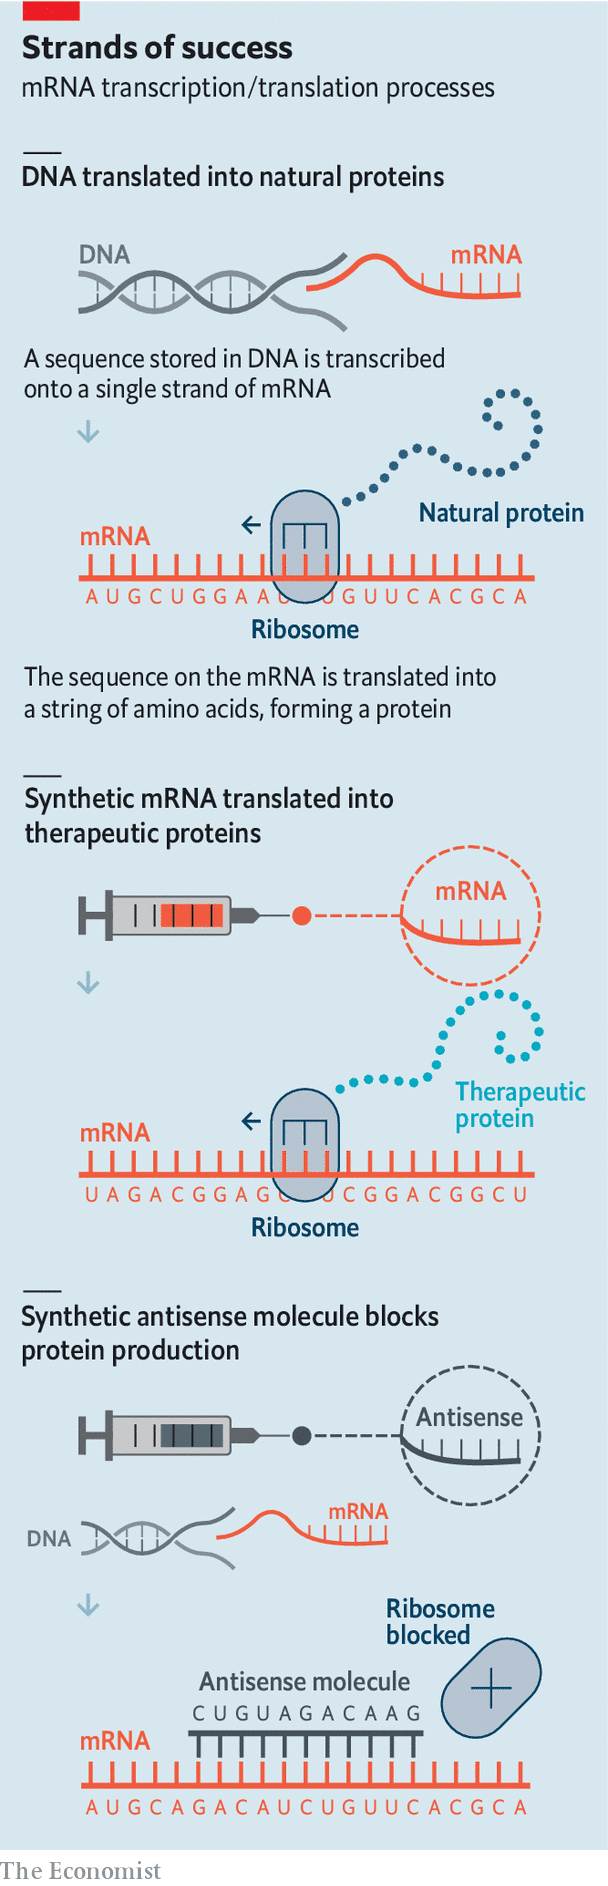
\includegraphics[width=0.4\textwidth]{images/20210327_FBC001.png}
\end{figure*}


The end of the mRNA molecule is formatted into a distinctive shape which is recognised by ribosomes, complex pieces of machinery composed of dozens of proteins draped around another set of RNA molecules. With the help of yet more RNA molecules---little ones called tRNAs which stick to the mRNA sequence three letters at a time---the ribosome translates the genetic message into the protein it refers to by creating a chain of amino acids as it moves along the message. 

This is the mechanism exploited by the RNA vaccines developed by BioNTech, a German biotechnology company based in Mainz, and Moderna, an American one from Cambridge, Massachusetts, against SARS-CoV-2, the virus which causes covid-19. The companies mass produce the RNA sequence describing the distinctive ``spike'' protein, which studs the outer membrane of the virus, formatted so as to look like a natural mRNA. These RNA molecules, wrapped in little fatty bubbles called liposomes are injected into patients, where the liposomes smuggle the mRNA into cells. Ribosomes pick up on the mRNA format and read the sequence, thus producing the spike protein. The immune system learns to recognise the spike which the vaccinated cells are producing and stores away the memory of how to do so. This allows it to mount a swift response if it later comes across the same protein on the surfaces of viral particles and infected cells. 

This ability to get cells to churn out proteins for which their DNA contains no genes is, in itself, enough to open up swathes of new therapeutic territory. But it is not the whole story. Cells make vast amounts of RNA that does not describe proteins. Its ability to recognise specific genetic sequences makes it useful for all sorts of processes, including turning the translation of genes on and off. Its ability to fold itself into particular forms---hairpins, loops and the like---makes it good at interacting with proteins. 

This alphabet soup of RNAs (see table) seems to function a bit like a computer's operating system, mediating the relationship between the cell's hardware and its software. Many of the details of how this works remain obscure. But some are understood well enough for a lot of brainpower and money to have been poured into attempts to hack the operating system for therapeutic purposes. 

These abilities should enable drugmakers to head upstream from the proteins whose shapes they have long studied into the realms of sequence. Where previously they targeted proteins which were already present, now they can in principle target the processes which control which proteins get made in the first place, adding helpful new ones to the roster and crossing harmful old ones off. There are RNA-based drugs in clinical trials for the treatment of cancer, heart disease and numerous inherited disorders---as well as brain diseases such as Alzheimer's and Parkinson's. 

Moreover, RNA's mixture of sequence and shape means that in many of these areas the once-haphazard process of drug discovery, long dependent on matching the shape of small synthetic molecules to the crannies and crevices of the proteins they targeted, can itself be systematised. A sequence which recognises, or forms a part of, one gene can be switched out for a sequence tailored to another. When what an RNA drug does depends on its sequence, its target and action can be modified by the click of a mouse. 

Both the firms with mRNA vaccines on sale had other vaccines in the pipeline before covid-19 struck. It is part of the appeal of the technology that they were able to turn on a sixpence and refocus their efforts on SARS-CoV-2 as soon as the sequence for its spike gene was released last January. Now they are both getting on with what they had planned beforehand. Moderna is looking at vaccines to fend off infection by cytomegalovirus (a herpes virus which causes neurological problems in newborns), three lung viruses which cause respiratory disease in young children and Zika, a mosquito-borne virus found mainly in the tropics. BioNTech is focusing more on developing vaccines, and other treatments, with which to treat a wide range of cancers. 

Cancer cells tend to have peculiar constellations of proteins on their surfaces, including both normal ones that are overexpressed and, more intriguingly, mutant forms peculiar to the development of that tumour. Comparing the genes expressed in a patient's healthy cells with those used by their tumour cells reveals which mutant proteins the cancers are producing; mRNAs for those proteins can then be incorporated into a vaccine. 

 

Produced as a result of vaccination, the proteins can engender a vigorous immune response the cancer itself does not---part of being a successful tumour is deploying mechanisms that stop the immune system from coming to grips with you. According to Ozlem Tureci, BioNTech's co-founder, the firm has 500 patients enrolled in clinical trials for cancer. Moderna is pursuing similar ideas. 

BioNTech is also testing mRNA vaccines aimed at overexpressed but unmutated proteins. Moderna, meanwhile, is looking into vaccines that train the immune system to recognise proteins created by common mutations in KRAS, a gene implicated in about 20\% of human cancers. CureVac, based in Tübingen, an mRNA firm which also has a SARS-CoV-2 vaccine in trials, is conducting trials of a vaccine for non-small-cell lung cancer. 

Vaccination is not the only way that mRNA injection might fight viruses and tumours. The technique could also be used to get cells to produce therapeutic proteins that are currently administered through injection or infusion: interleukins and antibodies. Designer antibodies are a massive faff to make in industrial quantities; getting patients' cells to take on the manufacturing duties instead would be a great step forward if it proved practical. 

There are many other sorts of proteins which can be stimulated to therapeutic effect. A project on which Moderna is collaborating with AstraZeneca, a pharmaceutical giant, delivers the mRNA for a protein which encourages the regrowth of blood vessels. The idea is that the therapy, now in phase 2 clinical trials, could stimulate the growth of new cardiac blood vessels after heart attacks. 

Getting the body to produce a protein it needs just for a short while---an antibody, say, or a growth factor---is one thing. But what about a protein that it needs on an everyday basis, but lacks the gene for? Such genetic diseases have always been the most obvious targets for gene therapy---treatments which add a missing gene to a patient's cells, or repair a broken one, thus allowing them to make a protein they have hitherto lacked. But at least some such conditions might instead be treated with mRNA. Inserting a gene might be more elegant---but getting it in the right place and regulated in the right way is challenging. If mRNA treatments get the job done, they might offer a nice alternative. 

There are thus mRNA treatments being studied for phenylketonuria, a metabolic disorder which requires sufferers to restrict their diets for their entire lives; glycogen-storage disease, which enlarges the liver and kidneys and stunts children's growth; and propionic and methylmalonic acidemias, two illnesses in which the body cannot properly break down proteins and fats. All are conditions that gene therapists are looking at, too. 

That BioNTech, Curevac, Moderna and some others now have all these projects on the go is largely down to the fact that they have spent many years developing the basics of their platforms. Many hurdles had to be crossed before they could get cells to accept and act on messages from beyond; the RNA had to be subtly toughened up so that it would not itself fall prey to the immune system or get dismantled inside cells; the right lipids had to be found for delivery, sometimes tailored to particular tissues like those of the liver or lymph nodes. The potential inherent in the idea meant that their work was not completely ignored; in 2018 Moderna's IPO valued the company at \$7.5bn, a record for the biotech sector. But biotechnology has a long history of proving biology to be messier and more contrary than those seeking to exploit its loopholes expect. 

Scepticism was also warranted, it seemed, by the fact that messing around with RNA had been through bursts of popularity before. One of the very oldest companies in the field, Ionis Pharmaceutials (known as Isis until that name was appropriated by a would-be caliphate) was founded in 1989. Its intention, then and now, was not to make use of mRNA, but to hobble it. 

The sequence of an mRNA molecule carries the same information as can be found in the gene which served as its template; but thanks to the way RNA is made it carries it in a complementary way. Where the DNA has a letter called C for cytosine, the RNA will have G for guanine; where the RNA has a C the DNA will have a G, and so on. Complementary strands stick together; that is what keeps DNA molecules paired up in double helices. If you introduce an mRNA to a molecule with a complementary sequence the two will stick together, too, rendering the mRNA useless (see bottom deck of diagram above). 

Again, getting the neat idea to work in ways that helped proved hard. It took Ionis a quarter century to start getting its ``antisense'' drugs to market on a regular basis. It now has three: nusinersen, approved in America in 2016 and Europe in 2017 for use against childhood spinal muscular atrophy, a muscle-wasting illness; inotersen, approved in 2018 for hereditary transthyretin-mediated amyloidosis (hATTR), which damages the peripheral nervous system; and volanesorsen, approved in Europe in 2019, which lowers levels of triglyceride fats in the blood of people with a metabolic error that makes them far too high. 

Ionis currently has a further 37 antisense molecules in clinical trials for conditions including Huntington's disease (a study being carried out in collaboration with Roche, a large Swiss pharma company); amyotrophic lateral sclerosis, Alzheimer's disease and Parkinson's disease (in collaborations with Biogen, a specialist in treatments for neurological disease); beta thalassaemia, a blood disorder similar to sickle-cell anaemia; and cystic fibrosis. 

The firm is also developing, in collaboration with Novartis, another Swiss company, a way of reducing levels of lipoprotein(a), a particularly damaging form of low-density-lipoprotein (LDL) cholesterol. Lipoprotein(a) levels are untreatable with existing medicines; Pelacarsen, as the drug is known, is in phase 3 clinical trials to see if it can change that. 

Unlike molecules of mRNA, which can tolerate only a small amount of chemical tinkering before becoming ribosome-unfriendly, antisense molecules can be tweaked quite a bit, and thus made long-lasting. Ionis's researchers have worked out how to stabilise them so that they will hang around inside cells for months. This is important because most of Ionis's targets are chronic diseases that require continuous treatment. The fewer injections per year the better. 

While biotech companies were beavering away at antisense molecules in the 1990s, researchers elsewhere discovered that nature had a similar technology of its own: gene silencing, a process guided by small interfering RNAs (siRNAs). The early 2000s saw a gene-silencing biotech boom led by Alnylam, founded in Cambridge, Massachusetts in 2002, and Sirna Therapeutics, which got going in San Francisco the following year. 

Established pharma companies, including Abbott, Merck, Novartis, Pfizer, Roche and Takeda, waded in, too, with Merck buying Sirna for more than \$1bn in 2006. For almost a decade, attention and money were showered on the field. But though there were many promising leads, they failed to turn into drugs. By the early 2010s it seemed that the party was over. 

Alnylam, though, kept dancing. In 2014 it bought what was left of Sirna from Merck for a knock-down price. It launched its first product, patisiran, a treatment for hATTR, in 2018. It now has two others, givosiran and lumasiran, which also address rare genetic disorders. 

A fourth substance developed using its technology has broader appeal. This is inclisiran, developed to treat an inherited disorder that pushes the concentration of LDL cholesterol in the blood to dangerous levels; around 30m people worldwide suffer from it. A firm called the Medicines Company licensed Inclisiran from Alnylam to bring it to market. With approval looking likely (it was given in Europe late last year) Novartis bought the Medicines Company for \$9.7bn in January 2020. 

According to Akshay Vaishnaw, Alnylam's head of R\&D, the firm has another 14 siRNA drugs in clinical trials. These including potential treatments for haemophilia, hepatitis B and recurrent kidney stones. Arrowhead Pharmaceuticals, of Pasadena, California, has eight potential siRNA drugs in trials, including one directed at cystic fibrosis. Dicerna Pharmaceuticals, of Lexington, Massachusetts, has three. 

These siRNAs work by straddling the worlds of shape and sequence. Their shape fits them into a group of proteins called an RNA-induced silencing complex (RISC). But a bit of the siRNA is left sticking out of this complex; this tail contains a sequence complimentary to that of the RNA to be silenced. When siRNA and mRNA meet, the proteins in the RISC chop the messenger to pieces. (A conceptually similar mechanism for the RNA-guided protein-executed chopping up of genes found in bacteria is the basis of the CRISPR tools now revolutionising gene editing.) 

In plants and invertebrates the natural function of the siRNA mechanism is clear: cutting up mRNAs associated with viruses. They do not seem to serve that function in vertebrates, and no one is quite sure what they do instead. But that does not stop them from looking like promising drugs. 

So do another set of RNAs associated with RISCs: micro-RNAs, which use their complementary sequences not to destroy mRNAs but to regulate them. The human genome seems to contain about 2,600 of these miRNAs, and they are thought to be involved in regulating the rate at which about 60\% of the genes describing proteins get transcribed. Several look like promising therapeutic targets. 

Since the active bit of an miRNA is a single-stranded sequence-specific tail, the obvious way to target them is with antisense. Regulus Pharmaceuticals, a firm that started life as a collaboration between Ionis and Alnylam, is trying to develop antisense molecules aimed at miRNA-21 to treat two kidney-related genetic conditions in which that miRNA plays a role. When you start targeting miRNAs, though, things get positively baroque. Santaris Pharma, a Danish firm, has developed Miravirsen, an antisense suppressor for miRNA-122 which the hepatitis C virus uses for its own unhelpful ends. The drug has now been taken on by Roche. 

The innovation continues. MiNA Therapeutics, a startup in London, is working on the potential of saRNAs, which activate genes which otherwise stay silent. Others are investigating systems for ``self-amplifying'' mRNA drugs. These mRNAs would inveigle a cell's ribosomes into producing not just the protein that was meant to be delivered, but also a second protein, called RNA-replicase, which would make more of the mRNA, thus leading to even more protein being expressed. There is surely further cleverness to come. 

\begin{figure*}[h]
\centering
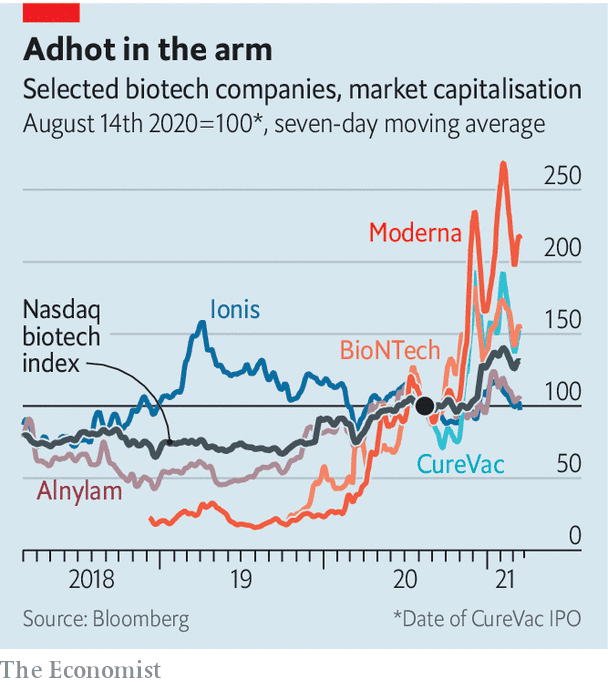
\includegraphics[width=0.4\textwidth]{images/20210327_fbc310.png}
\end{figure*}


Even if only a fraction of these possibilities pan out it looks certain that, in popularity contests to come as in stockmarkets today (see chart), more people will be plumping for RNA. Their support will be welcomed by the small band of biologists with an interest in the very earliest history of life that has long formed the discerning core of the molecule's following. Life needs both a way of doing things in the now---catalysing the reactions on which its metabolism depends---and of passing information into the future. Of the molecules known today only RNA, in its shape-and-sequence versatility, can do both those things, dealing with the needs of the everyday at the same time as encoding instructions for its own reproduction in the form of a legible sequence. This suggests to many that early life spent some time in an ``RNA world'' before the division of labour allocated doing things to the proteins and storing data to DNA, reducing RNA to a supporting role in the world it had created. 

The application of RNA has met many obstacles over past decades, and the fact that it has proved itself in vaccines does not mean it will not meet more in the future. But it does seem that medicine now has a way to target drugs not just at proteins, but at the processes that make them, and that opens up new realms of possibility. The next RNA world awaits. {} 

\textbf{Dig deeper} 

\emph{All our stories relating to the pandemic and the vaccines can be found on our \href{/news/2020/03/11/the-economists-coverage-of-the-coronavirus}{coronavirus hub}. You can also listen to \href{/podcasts/the-jab-a-new-podcast-from-the-economist}{The Jab}, our new podcast on the race between injections and infections, and find trackers showing \href{https://www.economist.com/graphic-detail/tracking-coronavirus-across-the-world}{the global roll-out of vaccines}, \href{https://www.economist.com/graphic-detail/coronavirus-excess-deaths-tracker}{excess deaths by country} and the virus's spread across \href{https://www.economist.com/graphic-detail/tracking-coronavirus-across-europe}{Europe} and \href{https://www.economist.com/graphic-detail/tracking-coronavirus-across-america}{America}.} 
\clearpage
\section{United States }
\subsubsection{Violence in America }
\subsection{In 2020 America experienced a terrible surge in murder. Why? }
\paragraph{Print Edition | United States  \quad \color{gray}{Mar 27th 2021 }}
\begin{figure*}[h]
\centering
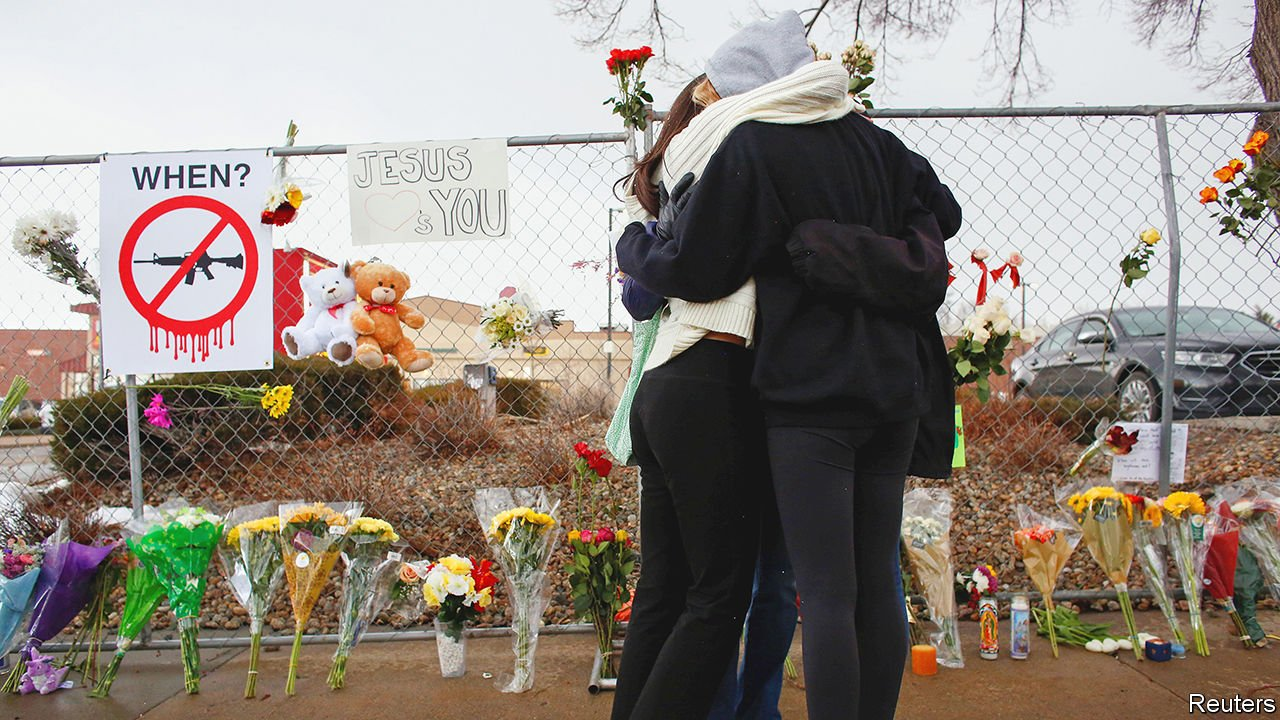
\includegraphics[width=0.8\textwidth]{images/20210327_USP001_0.jpg}
\end{figure*}
\lettrine{I}N MANY RESPECTS, the murder of Alante Hands last year on a Chicago street was sadly unremarkable. He was young, just 27, and black, like four in every five homicide victims in the city. Like nine in ten murders in Chicago, his life was taken by a gun---bullets pierced his arm, chest and leg. He had a lengthy criminal record, beginning a decade ago when he was arrested while still a minor for shooting at a police officer. He died in the violent West Side of the city on West Rice Street, where six others have been murdered in the past two decades. But for the fact that his murder occurred on December 31st 2020, the 787th and final one of an especially bloody year for the city, it might have been forgotten. 

The plague year proved brutal for Chicago, already a violent city even by American standards. Murders increased by 56\% from 2019---nearly three times as many victims as in all of Italy. As crime data from 2020 are compiled, one thing has become clear: American cities saw the biggest rise in homicides in decades, currently estimated at 30\% in a single year. That would be the highest annual increase in more than 50 years. In New York City, murders were up by 45\%. In the Bay Area around San Francisco, they rose by 36\%. In Washington, DC, they climbed by 19\%. Our analysis of preliminary data from the FBI suggests that it is not just a big-city phenomenon. Small towns and even rural counties experienced smaller yet sizeable increases in murder rates (see chart). 

Neither does the increase appear to be subsiding. Homicides in New York City are proceeding at the same pace as the previous deadly year. Mass shootings, which were mercifully rare during the year of lockdowns, have returned. On March 16th, a spree of shooting at three massage parlours in Atlanta killed eight people. On March 22nd, ten were killed at a grocery store in Boulder, Colorado (pictured); President Joe Biden called for stricter gun-control laws. Though such shootings account for very few of the tens of thousands of annual gun homicides in America, they focus media attention on the enduring problem of violence. That could be salutary. Unlike past escalations in violence, this one has gone comparatively unremarked on by national politicians, despite its magnitude. 

\begin{figure*}[h]
\centering
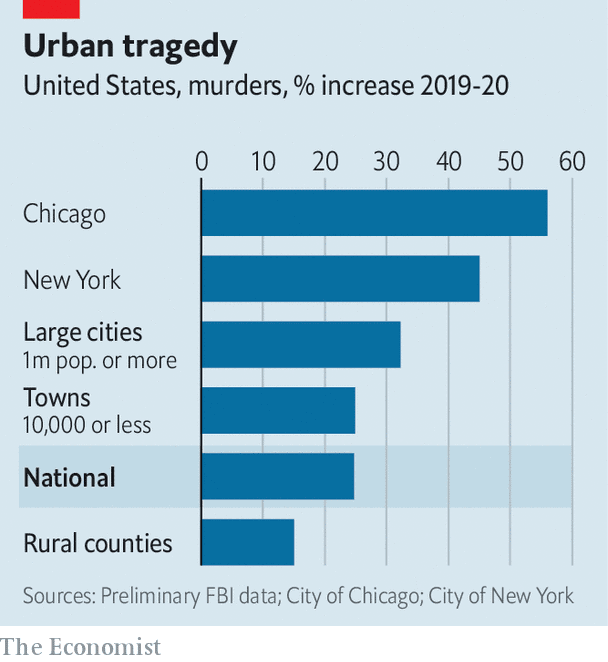
\includegraphics[width=0.4\textwidth]{images/20210327_USC300.png}
\end{figure*}


America benefited from decades of what researchers termed the ``great crime decline''---the violent-crime rate was cut nearly in half from 1993 to 2019. If that 30\% rise in city murders in 2020 were to hold nationwide, it would return America to a homicide rate last experienced in 1998. ``It's like 20 years of crime decline and violence decline has just disappeared,'' says John Roman, a criminologist at NORC, a research institute at the University of Chicago. 

What has caused this? One theory emphasises the pandemic. ``The recipe for violence in any city in the world is dense clusters of young men with nothing to do,'' says Mr Roman. Schools, work, churches, community centres and violence-cessation programmes all stopped, making it easy for conflict to escalate. 

The dwindling of stimulus payments over the summer meant that poverty was rapidly increasing during the months when murder spiked. Patrick Sharkey, a sociologist at Princeton University, notes that sales of guns and alcohol, common precursors to violence, soared. Some 23m guns were bought in 2020, 64\% more than usual. Alcohol sales were up by 25\%. Drug-overdose deaths probably hit another peak in 2020; competition over illicit-drug sales often spills over into violence, perhaps offering a partial explanation for the simultaneous increase in rural America. Pandemic effects may thus may provide all the ingredients for the year's grim cocktail. 

Another explanation identifies the killing of George Floyd in Minneapolis on May 25th, and the ensuing national protests, as the turning-point. Paul Cassell, a law professor at the University of Utah, suspects a nationwide ``Minneapolis effect''. Murder had been high throughout the year, but it did seem to surge around that time. In Chicago, 42 people were killed between May 27th and June 2nd, the deadliest week in the city since 2001. 

This theory holds that a sudden shock in the behaviour of cops, as officers are diverted to secure protests and discouraged from proactive policing, leaves a vacuum in high-crime neighbourhoods. Arrests in New York City dropped between July and September, even though these were the deadliest months in the city in years (and arrests were down by 35\% for the entire year). Loss of trust in the police may also exacerbate violence. American cities that have experienced large protests over police practices have often experienced a subsequent wave of violence. In Baltimore, after the death of Freddie Gray in police custody in 2015, homicides rose by 50\%, and have remained stuck near there ever since. 

A puzzle, particularly for the pandemic explanation, is America's exceptionalism in rising murders---unlike the country's great crime decline, which coincided with global drops in violence. Most countries went into pandemic-induced lockdown, and many have emerged with stagnant or even lower murder rates. Murders in Italy dropped sharply, and those in England seem to have remained flat. Even in the violent neighbouring country of Mexico, murders did not increase. The same was true of most of the Americas. 

If the primary causes are pandemic-related, that may augur a reprieve in the coming summer months as vaccination drives fully reopen the economy. If they are instead related to a crisis in policing, the effects could well linger, as in Baltimore. 

Crime is often seen as a local phenomenon, the province of mayors and not presidents. The synchronous rise of homicide across American cities and towns suggests a national problem, however. As the White House has been consumed by other crises---covid-19 and now immigration---rising violence has not been a focus of the Biden administration. Should it persist, however, the trend will become increasingly hard to ignore and could disrupt the politics of criminal justice. Progressives calling to defund police or otherwise minimise police presence may find their arguments harder to sustain. 

Things certainly do not seem to be improving in Chicago. Compared with last year, murders are already up by 11\%. {} 
\clearpage
\subsubsection{Politics, unions and Amazon }
\subsection{Amazon could get its first unionised workforce in America }
\paragraph{Print Edition | United States  \quad \color{gray}{Mar 27th 2021 }}
\begin{figure*}[h]
\centering
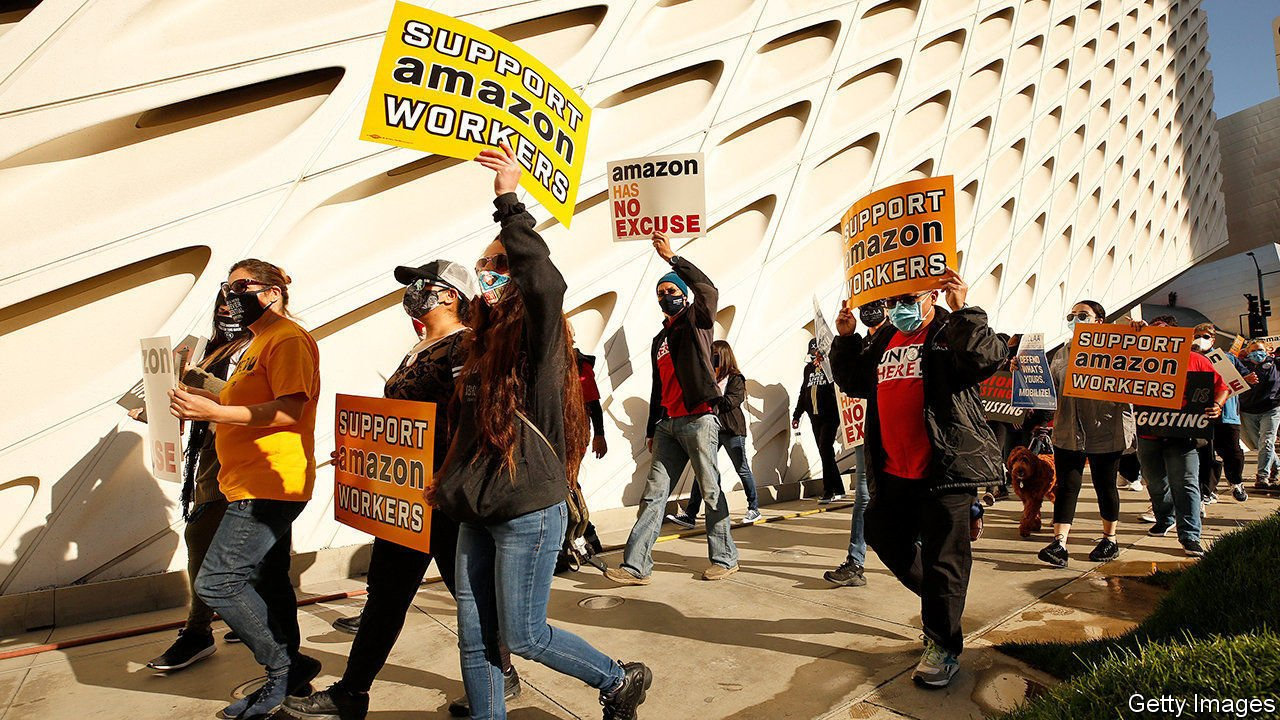
\includegraphics[width=0.8\textwidth]{images/20210327_usp503.jpg}
\end{figure*}
\lettrine{D}ARRYL RICHARDSON is proud of making his call. One of nearly 5,800 workers at an Amazon warehouse in Bessemer, Alabama, he says he was the one who first phoned the Retail, Wholesale and Department Store Union (RWDSU) to ask it to organise his fellow workers. As a result, since February, staff have been voting in a mail-in ballot. After that concludes on March 29th, Bessemer may become a unionised plant, Amazon's first in America after a quarter-century of operations. 

The result is uncertain, but the campaign is popular: sympathetic drivers honk as they pass placard-waving activists standing in the spring sunshine outside the Amazon plant. Barely 10\% of American workers today belong to a union but, according to Gallup, a pollster, 65\% of Americans approve of labour unions. They were last so well-liked back in 2003. One of the activists calls the battle in Bessemer a ``David and Goliath'' fight, and says the little guy might just win. 

Stuart Appelbaum, head of the RWDSU, says this vote transcends efforts at a single warehouse. It has drawn national attention---out-of-state politicians and activists have for months flocked to stand on the roads outside the warehouse to show their support. Public understanding of hardships faced by front-line and essential workers in the pandemic has spread sympathy. Mr Appelbaum speculates that the vote could help shape ``the future of work''. 

That may be overstating it, but other youthful workers, notably in the tech and retail industries, are gripped by the contest. Workers at Amazon plants across America, Mr Appelbaum says, have been in touch to say they may follow Bessemer's lead. And for some African-Americans, the campaign is seen as part of a wider push for better treatment. In Bessemer most workers are black and around half commute from nearby Birmingham, a city with a grim history of mistreating labourers, including prisoners who used to be hired out cheaply to toil for private employers. 

The vote is happening at a moment that looks unusually ripe, politically, for unions. Organised labour has an outspoken champion in the White House. Joe Biden, who kicked off his presidential run from a union hall in Pittsburgh, vowed to be ``the most pro-union president'' ever. In February he released a video---timed to boost the unionisation effort in Bessemer---saying that ``every worker should have a free and fair choice to join a union''. 

This week the Senate confirmed Marty Walsh, a former labourer and mayor from Boston, as his labour secretary, the first time in decades an ex-union boss has held that job. Mr Biden's administration also supported farmworkers' unions in a case before the Supreme Court this week. The court is to decide whether to undo a 45-year-old law in California that lets unions organise, uninvited, by entering farmers' land. Donald Trump's administration had backed two agricultural firms that are seeking to scrap the law, saying it unfairly punished companies. Mr Biden wants to keep it. 

The Biden administration is also supporting the PRO Act, a union-friendly bill that passed the House this month, after languishing in Congress for over a year. It drew only a handful of Republican backers and is widely opposed by employers, but a poll suggests that 59\% of the public favour it. The act would strengthen the powers of the National Labour Relations Board, grant independent workers more rights to organise and weaken provisions that exist in many states---known as ``right to work'' laws---that discourage union activity. 

The Senate almost certainly will not take it further. But Mr Biden's promotion of it looks well-judged politically. Doing so helps him fend off leading Republicans who themselves have offered pro-union statements. Josh Hawley, a senator from Missouri, declared in November that Republicans were now a ``working-class party''. Marco Rubio, from Florida, said this month that he supports unionisation at Amazon because the firm had waged a ``culture war against working-class values''. (Republicans also heartily dislike Jeff Bezos, Amazon's billionaire boss, who also owns the \emph{Washington Post}.) Neither, however, backs the PRO Act, or the idea of unionisation at other firms. 

Dan Kaufman, who has written on the politics of anti-union movements, says such pro-union comments by Republicans count as a mere ``performative tribute to the working class''. Yet even tributes can have appeal. Mr Trump managed to draw votes from a healthy 40\% of union households last year. Mr Biden outperformed him, winning 56\% support of union voters. But Mr Biden knows that getting support from union homes is no longer easily guaranteed for Democrats as once it was. 

Back in Bessemer, the mood is triumphant. Jennifer Bates, one of the union organisers, believes the labour movement has already won a victory regardless of the outcome of the vote. ``We have woken up a giant,'' she says. {} 
\clearpage
\subsubsection{Jobless data }
\subsection{Why jobless-claims data give little insight into America's economy }
\paragraph{Print Edition | United States  \quad \color{gray}{Mar 27th 2021 }}
\begin{figure*}[h]
\centering

\includegraphics[width=0.8\textwidth]{images/20210327_USP004_0.jpg}
\end{figure*}
\lettrine{I}N THE PAST year pundits have closely tracked America's ``jobless claims'' data, published every Thursday by the Department of Labour to show how many people are newly claiming unemployment insurance (UI). These data once provided invaluable insights: in 1995 Alan Greenspan, then chair of the Federal Reserve, personally intervened to ensure that they continued to be produced during a government shutdown. Yet in the current crisis more people are starting to realise their limitations. 

Somebody seeking UI benefits must file a claim with a state employment office. The claims data were useful early in the pandemic. They are published with a lag of only a few days, so gave an insight into the economic collapse of last March and April long before the monthly jobs report. In those two months claims data suggested that about 30m Americans had filed for UI---in line with later figures on job losses from the Bureau of Labour Statistics. 

Yet in the past year more than 80m applications have been filed for state UI. Were all applications unique, the data would imply that 50\% of American workers had lost their pre-pandemic job. Really? About 20m Americans remain on some form of UI, twice the number officially classified as unemployed. Initial claims for state UI have fallen from the heights of last spring, but even now over 700,000 claims are being filed each week, more than at the height of the financial crisis of 2007-09. 

It is possible the claims data reveal that America's labour market is doing far worse than other statistics show. More likely, the data themselves are flawed. 

Why? Early in the crisis wonks warned that initial-claims data would run high long after actual job losses had fallen, because state UI offices were catching up on backlogged applications. A paper last year from the Federal Reserve said ``errant claim duplication'' may inflate official tallies. Some state offices have made it easier for people working reduced hours---rather than not at all---to claim UI. The government has also allowed more people, including the self-employed and gig-economy workers, to be eligible for payments. Another source of distortion could be widespread fraud. 

No one knows the biggest reason why claims are so absurdly high. But this much is clear: to get the measure of America's labour market, look elsewhere. 
\clearpage
\subsubsection{Patronage games }
\subsection{Why is it so hard for Joe Biden to hire people? }
\paragraph{Print Edition | United States  \quad \color{gray}{Mar 25th 2021 }}
\begin{figure*}[h]
\centering

\includegraphics[width=0.8\textwidth]{images/20210320_usp505_0.jpg}
\end{figure*}
\lettrine{A}LL AMERICAN presidents are empowered to appoint thousands of true believers to turn their campaign promises into policy. But all modern presidents have struggled to get these people into their jobs. Joe Biden is no exception, at least when it comes to the roughly 1,100 appointees who require Senate confirmation. By March 24th, two months into his administration, after Rachel Levine, nominated as assistant secretary of health, became the first openly transgender federal official to win Senate approval, Mr Biden had obtained the confirmation of just 27 people. That puts him slightly ahead of where Donald Trump was at this point, but behind Barack Obama (see chart). 

America has far more political appointees in its federal government, some 4,000 in all, than any other developed democracy, according to David Lewis, a political scientist at Vanderbilt University. No one ever really stops to wonder whether, if so many roles can sit empty, all these jobs are needed in the first place. 

Presidents used to be free to hand out every job in the government. But in 1881 a spurned office-seeker assassinated President James Garfield. His successor, Chester Arthur, signed into law the act creating the civil service and, with it, the seeds of a permanent bureaucracy that would grow from administration to administration, developing many fine public servants along with an unknown quantity of rot. 

\begin{figure*}[h]
\centering
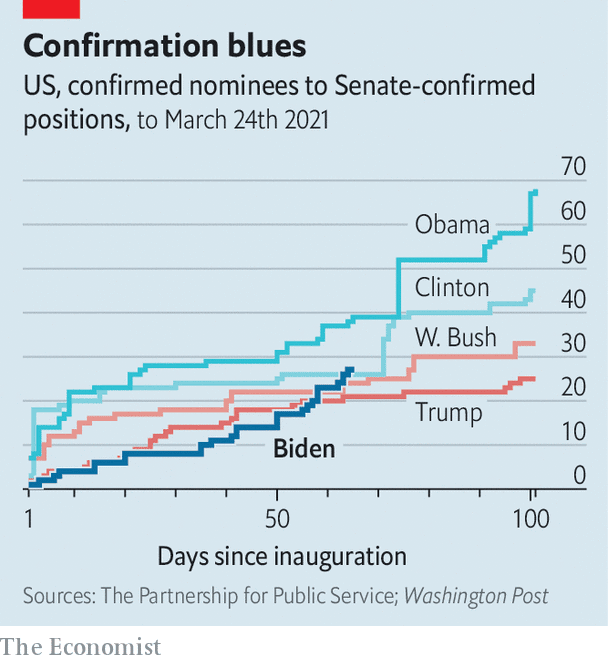
\includegraphics[width=0.4\textwidth]{images/20210327_usc258.png}
\end{figure*}


To advocates of the system, preserving a large number of senior positions for presidential appointment to manage the vast bureaucracy makes sense. It should create more accountability, bring new energy and expertise into government, give officials in outlying departments or embassies a direct line to the White House and expose more citizens to public service. But things have generally not worked out that way. 

One reason is that the Senate, especially when controlled by the rival party to the president's, can be hostile to an administration and its appointees. Another is that presidents, and the people they succeed in appointing, tend to get very busy right away with matters besides hiring. A study in 2010 by Mr Lewis and a colleague, Nick Gallo, found that appointees were reliably worse managers than career officers---and those that came from presidential campaigns or political parties were the worst. 

Every appointment is a wrangle. Interest groups mobilise to push their candidates; campaign donors work the phones to plead for ambassadorships; sometimes a senator blocks a nomination for a time, to gain leverage against the White House over some distantly related matter. It took Mr Obama an average of 510 days, and Mr Trump an average of 525 days, to get each assistant secretary of state confirmed, according to the Partnership for Public Service, a non-profit group. 

Wise in the ways of Washington, the Biden people anticipated the glacial Senate confirmation process and came up with a novel workaround. They had more than 1,000 appointees who didn't require confirmation ready to go as soon as the president was inaugurated. In this category of jobs, that puts Mr Biden far ahead of both Mr Trump and Mr Obama. 

But Mr Biden's hack of the appointments process will carry him only so far. In the departments and agencies, the top positions generally require Senate approval. Acting and career officials may fill some of the vacancies, but until a confirmed leader arrives to make decisions they are just warming the seats. This is said to be the case now at the \href{/united-states/2020/11/21/two-new-reports-provide-a-road-map-for-reforming-american-diplomacy}{State Department}, which, across the government, has the \href{/international/2020/08/13/the-dereliction-of-american-diplomacy}{largest number of vacancies} that must be filled with Senate-confirmed appointees. 

The secretary of state, Antony Blinken, \href{/united-states/2021/01/23/back-to-the-future}{sprinted to confirmation} back in January. But he does not yet have an under-secretary for arms control and international-security affairs to advise him on dealing with Russia or \href{/asia/2021/01/09/is-north-koreas-dictator-losing-his-touch}{North Korea}. He has no under-secretary for civilian security, democracy and human rights, nor a co-ordinator for counterterrorism or chief of protocol. The administration has yet to nominate, let alone secure confirmation for, any of the 22 assistant secretaries. Dozens of embassies lack an ambassador, each of whom must be confirmed by the Senate. 

In 2020 only 21\% of the posts of assistant secretary or above were held by career officials, compared with 60\% in 1975, according to the Partnership for Public Service. A similar though less extreme trend has shifted the balance of ambassadorships towards political appointees. The Biden administration has indicated it intends to reverse these trends by appointing more career diplomats to senior posts. 

But that means disappointing more donors and other supporters, raising the stakes even further for each choice that remains in the president's gift. Add to this consideration the priority Mr Biden places on diversity and the reality of how homogenous the ambassador corps is---only five of 189 ambassadors are black---and the maths become even more complex. 

Mr Blinken got some good news last week: one of his deputies, Brian McKeon, finally cleared the Senate. Mr McKeon's remit is resources and management. He has his work cut out for him. {} 

\textbf{\emph{See also:}} \href{https://www.economist.com/tracking-joe-biden}{\emph{We are tracking the Biden administration's progress in its first 100 days}} 

\emph{A version of this article was published online on March 21st 2021} 
\clearpage
\subsubsection{Fashion police }
\subsection{A new dress code means Rhode Island lawmakers have to suit up }
\paragraph{Print Edition | United States  \quad \color{gray}{Mar 27th 2021 }}
\begin{figure*}[h]
\centering

\includegraphics[width=0.8\textwidth]{images/20210327_USP003_0.jpg}
\end{figure*}
\lettrine{J} ONATHON ACOSTA wore a blazer with a \emph{guayabera}, a traditional formal shirt in the Caribbean, on his first day as a senator in Rhode Island's legislature. Since then he has worn informal attire, a better reflection, he says, of his mainly Latino constituents. He often wears knitted hats and cardigans. The only wardrobe rule said that people must be ``properly dressed''. That changed on March 23rd, when the chamber passed a new dress code stipulating ``proper and appropriate attire'', such as blouses and collared shirts with a jacket. 

Before the vote, during a lively debate last week in the Senate Rules Committee, Mr Acosta argued that the new rule ``connotes white collar, white people''. He wasn't elected to wear ``a costume'', he was elected to legislate. Dominick Ruggerio, the Senate's president, retorted that he found it offensive when people are not dressed appropriately. Cynthia Mendes, another senator, later observed that the new dress code appears at a moment when Rhode Island has more women and more minorities than ever. 

Dress codes are often a reaction to diversity, says Richard Thompson Ford, author of ``Dress Codes: How the Laws of Fashion made History''. Current trends are away from formality in the workplace; Mr Acosta's wardrobe is similar to that of a Silicon Valley boss. At the same time, the number of dress codes adopted or enforced by schools has increased. Before the pandemic, reports of children being punished for their dreadlocks prompted Cory Booker, a black New Jersey senator, to introduce legislation banning race-based hair discrimination. 

Not everyone sees the suit as oppressive. The Student Nonviolent Co-ordinating Committee, a civil-rights group from the 1960s, wore their Sunday best for protests. It was a symbol of defiance. ``The African-American in elegant attire was seen as a threat to white supremacy,'' says Mr Thompson Ford. 

Around two dozen other statehouses have some sort of dress code, as does Congress. Women have been told to cover up their bare arms in the chamber of the House. Some rules are unspoken. Sonia Sotomayor was reportedly advised to wear neutral nail polish to her confirmation hearings as a Supreme Court justice, to avoid scrutiny. After Alexandria Ocasio-Cortez wore big gold hoops at her swearing-in ceremony to Congress in 2019, she tweeted: ``Next time someone tells Bronx girls to take off their hoops, they can just say they're dressing like a congresswoman.'' 
\clearpage
\subsubsection{March meltdown }
\subsection{Snow drought is worsening the American West's water woes }
\paragraph{Print Edition | United States  \quad \color{gray}{Mar 25th 2021 }}
\begin{figure*}[h]
\centering
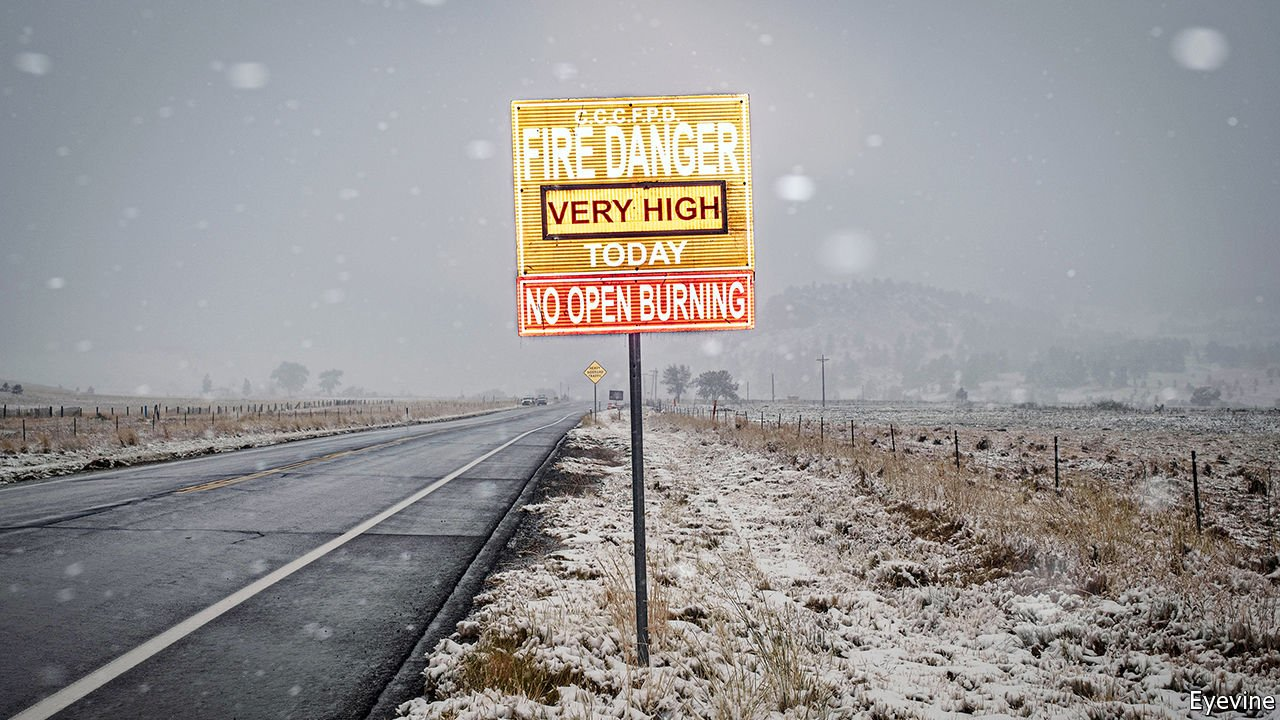
\includegraphics[width=0.8\textwidth]{images/20210327_usp002.jpg}
\end{figure*}
\lettrine{O}N MARCH 13TH Denverites watched from frozen windows as the fourth-biggest snowstorm ever to hit their city buried Colorado's capital two feet deep, and added fresh powder to the foothills of the Rockies. Local officials closed the main highway to the mountains to stop eager skiers getting trapped on icy roads on their way to the slopes. After a dry 2020 and a warm start to winter, the storm brought eastern Colorado's winter snowpack (the accumulation of snow) up to average levels. When it melts, water will replenish thirsty reservoirs, rivers and soil. But much of the Mountain West watched the snow falling on Denver with envy. 

Drought has afflicted a large swathe of the region for nearly a year (see map). The Colorado river basin, which includes pieces of seven western states and part of Mexico, has been among the worst-affected areas. A warm spring in 2020 led snow to melt early, which depleted the amount of water reservoirs and rivers received during the driest months of the year, in summer and autumn. The annual monsoons that the south-west depends on never came---and have been lacklustre for four years. The combination of the early melt and a hot, dry summer led to a deadly wildfire season. Colorado and California both suffered their biggest fires on record last year. 

Becky Bolinger, Colorado's assistant state climatologist, says multiple prolonged periods of drought since 2000 have made it impossible for the country's biggest reservoirs---Lake Mead in Nevada and Lake Powell on the border of Utah and Arizona---to recover fully. The lakes are now roughly two-fifths full. 

\begin{figure*}[h]
\centering

\includegraphics[width=0.4\textwidth]{images/20210327_usm942.png}
\end{figure*}


The blizzard that buried Denver did nothing to ease the drought on the other side of the continental divide. The Rockies split Colorado in two: the Front Range, with its high plains, and the Western Slope, where waters flow towards the Pacific. The Mountain Studies Institute, a research group in Silverton, estimates that western Colorado has warmed faster than any part of the country except Alaska. 

On March 24th snowpack in the south-western corner of the state was at 84\% of its normal level for this time of year. That may not seem too bad, but the region needed above-average precipitation this winter to make up for the past year. Citing a lack of snow, Utah's governor declared a state of emergency and urged Utahns to find ways to save water. The situation looks bleaker still farther south. Snowpack in parts of Arizona and New Mexico has fallen to less than 50\% of the seasonal average. 

 

Average snowpack has been decreasing for decades. Philip Mote, a professor of atmospheric sciences at Oregon State University, found in 2018 that annual snowpack in the American West has declined by 15-30\% since 1915. But studying snow drought (and indeed using the term itself) is a recent phenomenon, says Dan McEvoy, a climatologist at the Western Regional Climate Centre in Reno, Nevada. He reckons that warmer winters due to rising carbon-dioxide emissions have made the droughts more frequent and harder to ignore. A lack of snow deprives soil and forests of essential nutrients. It also increases river temperatures and can heighten the risk and severity of wildfires. Unstable snowpack also seems to have contributed to an increase in \href{https://www.economist.com/graphic-detail/2021/03/03/avalanches-have-been-particularly-deadly-in-america-this-year}{avalanche deaths} this year\textbf{.} 

\begin{figure*}[h]
\centering
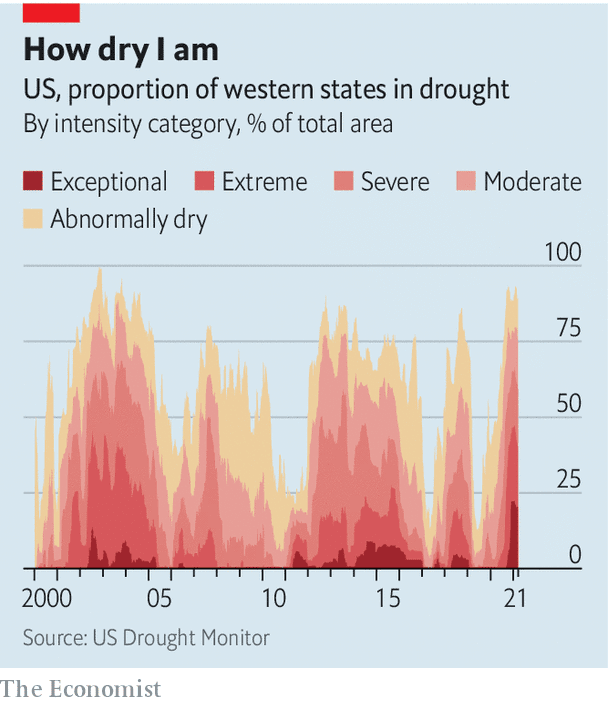
\includegraphics[width=0.4\textwidth]{images/20210327_usc266.png}
\end{figure*}


Not only the environment suffers for want of snow. The economies of many towns in the West are centred on the white stuff and the tourists that come in search of it. ``In the ski industry, snow is currency,'' says Auden Schendler, the vice-president of sustainability at Aspen Snowmass resort. Winter-sports tourism is a \$20bn industry in America. Snow drought is an existential threat. 

Because drought is a perennial problem in the West, adaptation has become a way of life. Some farmers in Colorado and the north-west are experimenting with farming without irrigation. Colorado's proposed covid-19 stimulus plan includes up to \$55m to fight drought and fire. 

But the future promises ever more complicated water problems. The compact governing the use of the Colorado river expires in 2026. The agreement, negotiated in 1922, called for ``upper basin'' states to share water equally with ``lower basin'' ones. It is showing its age. Today around 40m people depend on the river for water. States, tribes, the Mexican government, developers, environmentalists and farmers all want a say in how the water is allocated. The lower basin is also home to some of America's fastest-growing cities, such as Phoenix and Las Vegas. 

It would be hard enough to draw up a modern compact that satisfies so many competing interests. Add a shrinking water supply and growing populations, and a battle over the river looms. Individual states are getting ready for it. Utah has created a new agency to argue for more water on the state's behalf. The fight over water, much like the West itself, is heating up. {} 

\emph{For more coverage of climate change, register for The Climate Issue, our fortnightly \href{/theclimateissue/}{newsletter}, or visit our \href{/news/2020/04/24/the-economists-coverage-of-climate-change}{climate-change hub}} 

\emph{A version of this article was published online on March 23rd 2021} 
\clearpage
\subsubsection{America's new religious war }
\subsection{Religious fervour is migrating into politics }
\paragraph{Print Edition | United States  \quad \color{gray}{Mar 27th 2021 }}
\begin{figure*}[h]
\centering
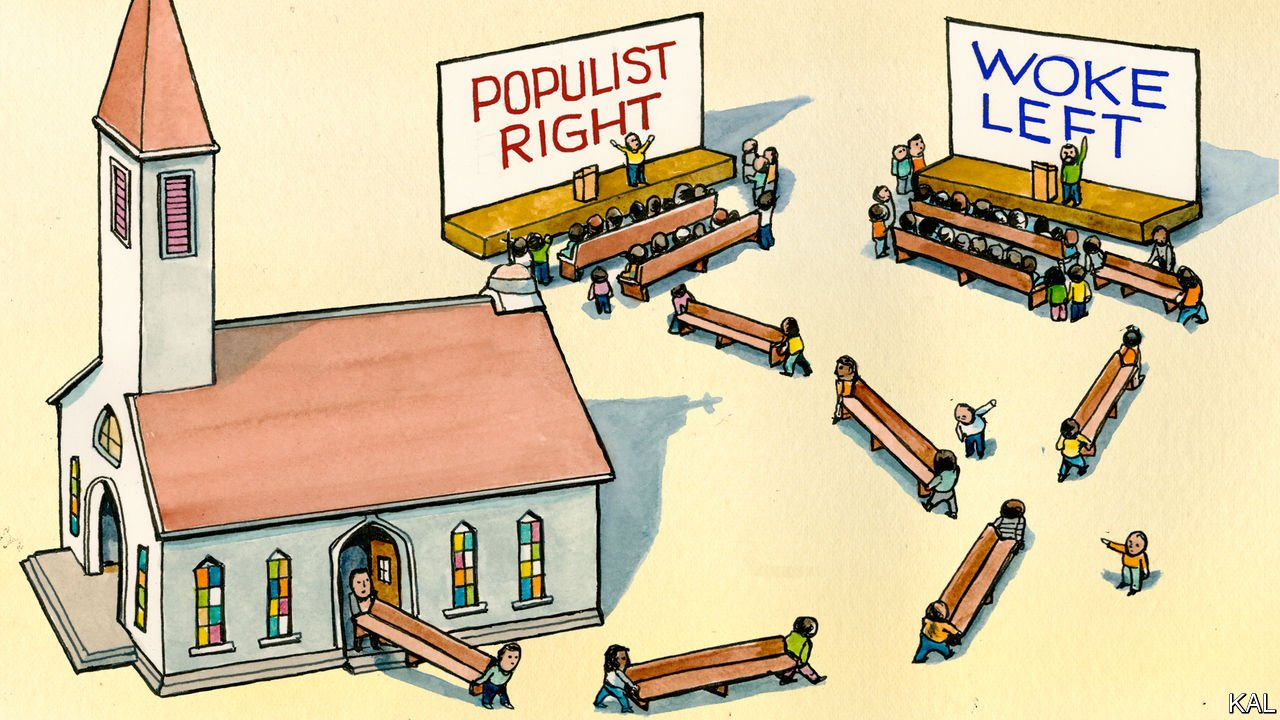
\includegraphics[width=0.8\textwidth]{images/20210327_USD000_0.jpg}
\end{figure*}
\lettrine{T}O START THE holiest week in the Christian calendar, Joe Biden is expected to attend Palm Sunday mass at Holy Trinity in Georgetown. He is the most religiously observant president since Jimmy Carter. Considering how organised religion is collapsing, this is yet another way in which his presidency is a throwback. 

He presides over a country in which more people claim to have ``no religion'' than to be Catholic or evangelical Christian. Yet unlike European countries, America is not becoming clearly less devotional as its churches retreat. Even Americans who have abandoned churchgoing are likelier to say they pray and believe in God than German or British Christians. They have rejected the institutions of religion, in other words, but not the religious urge---including a yearning for moral certainty and communal identity---that churches and synagogues have traditionally catered to. 

This is giving rise to a lot of heterodox thinking even within America's shrunken congregations. Nearly a third of self-described Christians say they believe in reincarnation. Wilder ideas are rising among the unaffiliated, as the theologian Tara Isabella Burton has described in ``Strange Rites'', a tour through the ``wellness'' cult, the ``brutal atavism'' of Jordan Peterson and the weird world of Harry Potter fandom. Politics looks increasingly like another such pseudo-religion. Righteous, moralistic, unforgiving and fervently adhered to, America's national debate has taken on a religious complexion in both parties. A new academic paper notes that since 2018 American Twitter users have been likelier to identify themselves by partisan affiliation than religion; on that platform especially, it has been a seamless switch. 

Some have hailed the displacement of religious fervour into the secular realm as proof of the ``God-shaped hole''. This is a conviction, attributed to Blaise Pascal, a French polymath of the mid-17th century, that the religious impulse can never be quelled. Human history suggests he was on to something. But it also suggests outbursts of religiosity owe as much to their cultural, especially institutional, context as metaphysics. The contrasting ways in which Republicans and Democrats are practising the new religious-style politics underlines the truth of that. 

The right might look more straightforwardly religious. Under Donald Trump, white evangelical Christians, a mainstay of the party for decades, became its most important group. But even if it includes some old-style values voters, this is no longer your father's moral majority. Most white evangelicals backed Mr Trump---more zealously than they had any previous Republican---mainly for cultural reasons that had nothing to do with Christianity. 

They were motivated far more by his immigration policies and racially infused law-and-order rhetoric than his judicial nominees. They have since shown little interest in Mr Biden's faith. Or in his efforts to restore the civic religion---an age-old idea of America as a nation blessed by God and united in moral purpose---that Mr Trump disdained. Around a third of white evangelicals subscribe to the QAnon cult. This was apparent in the prominence of man-sized crosses and other Christian paraphernalia among the cultists who stormed the Capitol Building on January 6th. 

This pseudo-religious makeover on the right was instigated by lapsed white evangelicals, who backed Mr Trump in the 2016 Republican primary when observant ones held back. Their continued self-identification as Christians, though they do not attend church, is often a proxy for ethno-nationalism. The same religious appropriation is evident, Tobias Cremer of Oxford University has shown, among Europe's Christian nationalists, who often do not even believe in God. Yet on the American right, unlike Europe's, it has received mainstream backing. Christian leaders, confusing the decline of their congregations with the cultural threat of liberalism, made common cause with Mr Trump and the pseudo-evangelicals. For partisan reasons, the rest of the Republican coalition followed them. The party has never been more avowedly Christian or more clearly out of line with gospel doctrines. 

The situation on the left is roughly the opposite. The most avowedly secular Democrats---well-educated ``woke'' liberals---are also the likeliest to moralise. Their Puritanical racial and gender politics sit in a long tradition of progressive Utopianism, rooted in mainstream Protestantism. Barack Obama's Messianic first presidential campaign was also in that vein. Yet these new Puritans of the left, though (or perhaps because) they are more secular than earlier progressives, are far more extreme. 

Their view of social justice has no place for forgiveness or grace---as Alexi McCammond recently learned, when the 27-year-old's editorship of \emph{Teen Vogue} was cancelled because of some bigoted Tweets she sent as a teenager. It is also more focused on purity and atonement within the liberal tribe (as that example also suggests) than making society less discriminatory. A clue to that is the fact that the Democrats' many African-American voters largely ignore such activism. They are more concerned to get better health care. Not coincidentally, many also still go to church. 

Woke liberalism is less prevalent than many conservatives claim. The Democrats would not have nominated the pious, grandfatherly Mr Biden otherwise. His pragmatic espousal of social justice is different in kind from the woke fringe. His appeals to America's better angels therefore went down with white liberals almost as badly as they did with white evangelicals. Yet on the cultural questions that now define American politics the Puritanical left is often as influential as the zealous right. 

No wonder political compromise has become impossible. Not since the 1850s, when New England's Puritans embraced the abolitionist case and southern Baptists preached a divine justification for slavery to thwart them, have politics and religion been so destructively confused. It is not a reassuring parallel. {} 
\clearpage
\section{The Americas }
\subsubsection{Fighting the P.1 variant }
\subsection{Brazil's mismanagement of covid-19 threatens the world }
\paragraph{Print Edition | The Americas  \quad \color{gray}{Mar 27th 2021 }}
\begin{figure*}[h]
\centering
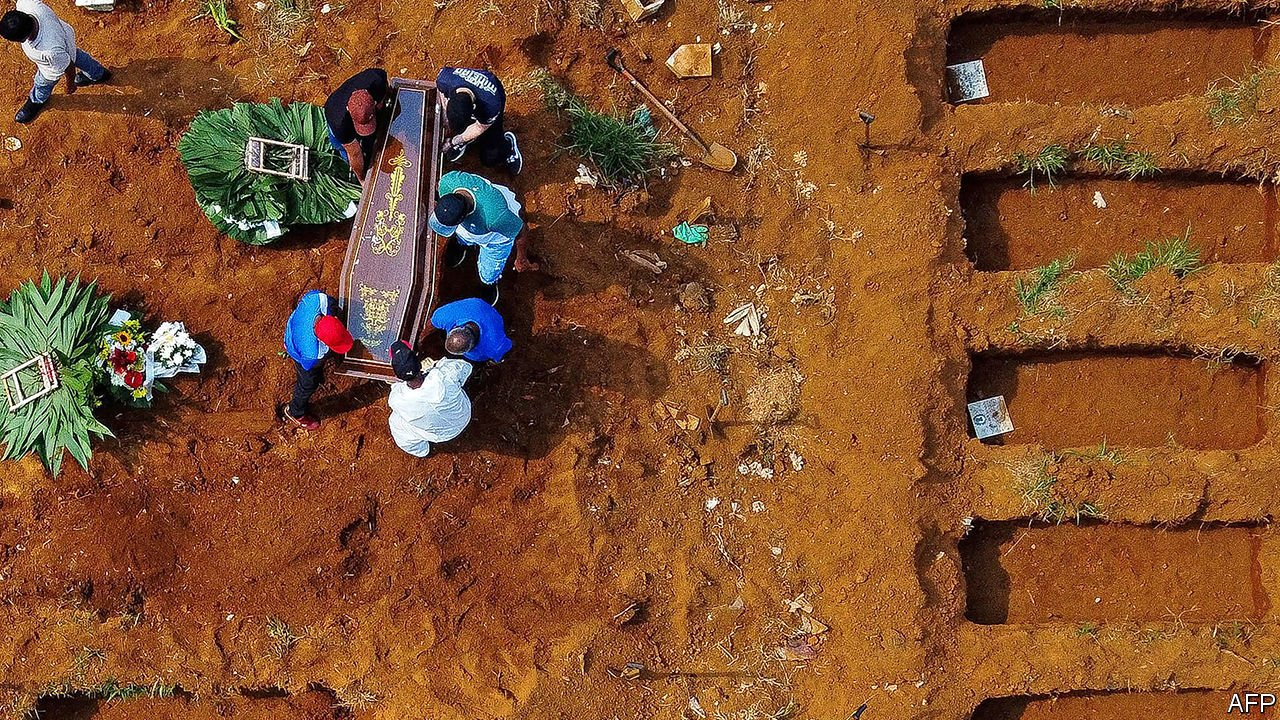
\includegraphics[width=0.8\textwidth]{images/20210327_AMP001_0.jpg}
\end{figure*}
\lettrine{S}éRGIO OLíMPIO GOMES, better known as Major Olímpio, was a policeman who entered politics 15 years ago. In 2018 he managed the campaign in the state of São Paulo of Brazil's current president, Jair Bolsonaro, and was elected to the national Senate. On March 18th this year he died of covid-19, aged 58. He is the third sitting senator to have died from the disease. Nearly 4\% of the legislature's upper house has perished in the pandemic. 

That has brought home to the political class a shock that millions of Brazilians are now experiencing. The country is suffering a second covid wave far worse than the first. Its recorded death toll, averaging over 2,300 a day, is a quarter of the world's total. This is despite the fact that Brazil has less than 3\% of the world's people. 

The health system is in a state of ``collapse'' for patients with severe cases of covid-19, says a bulletin published on March 23rd by Fiocruz, a public-sector research institute. In 25 of the 27 states more than 80\% of intensive-care beds are occupied. Eighteen states have shortages of drugs such as neuromuscular blockers, used when patients are put on ventilators. In six states oxygen supplies are dangerously low, according to the health ministry. The National Forum of Governors warns that shortages threaten to cause ``a collapse within the collapse''. 

\begin{figure*}[h]
\centering
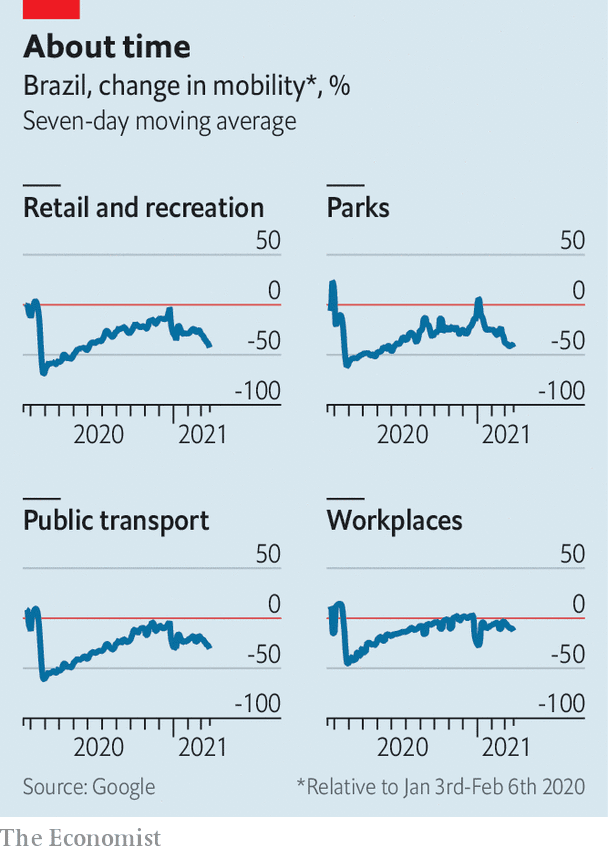
\includegraphics[width=0.4\textwidth]{images/20210327_amc276.png}
\end{figure*}


Bahia, a state in Brazil's north-east, is experiencing ``pressure'', not complete failure, says its health secretary, Fábio Vilas-Boas. But that is bad enough. The number of patients needing oxygen has ``exploded''. Some hospitals are treating covid-19 patients in emergency rooms because their intensive-care units (ICUs) are full. 

Brazil's second wave is thought to be mostly caused by a variant of the novel coronavirus, called P.1, which was probably born in the Amazonian city of Manaus. More contagious than the original, and able to reinfect people who have already had covid-19, P.1 has alarmed not just Brazil but the rest of the world. It has been detected in 33 countries. Some vaccines are less effective against P.1 than against other major variants of the virus in Europe and the United States. 

The country's neighbours are slamming shut their doors. Peru and Colombia stopped flights from the country. Just two of Brazilians' top ten destination countries remain open to them. ``If Brazil is not serious, then it will continue to affect all the neighbourhood there and beyond,'' warned Tedros Adhanom Ghebreyesus, the head of the World Health Organisation. 

But seriousness, like muscle blockers, is in short supply. Mr Bolsonaro has touted quack cures, railed against lockdowns and tried to thwart the publication of data. He has just bid farewell to the third health minister (an army general) since the pandemic began. Vaccines are not for him, Mr Bolsonaro has claimed. His government was slow to order them, even though manufacturers such as Pfizer and Janssen had tested them in Brazil. 

Governors and mayors, who implement lockdowns, have largely followed the president's lead. After clamping down at the beginning of the pandemic most quickly eased up. But even when restrictions are in place, Mr Bolsonaro's rhetoric can scupper their enforcement. In Bahia's poor neighbourhoods life has continued as normal, at least until very recently. ``We can't impose on those who live in favelas the obligation of being inside a hot small house,'' says Dr Vilas-Boas. The state does not have enough police to ensure that bars stay closed. 

That a variant like P.1 was born in Manaus comes as no surprise, says Natalia Pasternak, a microbiologist who leads Instituto Questão de Ciência, which advocates the use of science to shape policy. The city's first wave was so severe that some thought it had reached herd immunity. Residents thronged riverside beaches at the first opportunity, giving P.1 a fast start in life. When it left the forest, other parts of the country made it equally welcome. Although Brazil does too little gene sequencing to know for sure how widely it has spread, studies in São Paulo state identify the variant in 80-90\% of cases. 

\begin{figure*}[h]
\centering
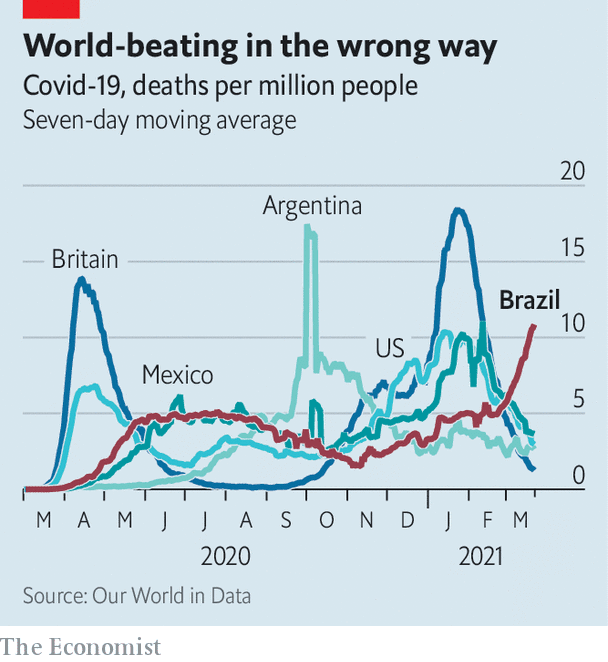
\includegraphics[width=0.4\textwidth]{images/20210327_AMC277.png}
\end{figure*}


P.1 is frightening because it may be both more contagious than earlier versions and able to reinfect people. One study suggested that it could be up to twice as transmissible and could reinfect 25-61\% of people who have had covid-19. P.2, a worrying variant from Rio de Janeiro, is also spreading. 

The shock of the second wave is changing people's behaviour. Governors and mayors are now tightening restrictions and people are obeying them more. From March 22nd a nightly curfew in Bahia begins at 6pm rather than 10pm. Bahians have recently cut in half the distance they travel, according to mobile-phone data. This is slowing covid-19's spread. Dr Vilas-Boas estimates that the number of active cases in Bahia has dropped from 21,000 to 17,000. The number of patients waiting for beds in ICUs fell from 513 on March 12th to 280 ten days later. 

This month the federal government finally agreed to buy Pfizer's vaccine and the one-dose jab from Janssen. They will supplement the AstraZeneca and Chinese CoronaVac vaccines already being administered. Brazil has begun domestic production, too. Fiocruz has delivered its first homemade doses of AstraZeneca; the Butantan Institute in São Paulo has begun making CoronaVac. Some 8\% of adults have had a first jab. ``For the first time,'' says Ms Pasternak, ``I'm hopeful.'' 

On March 23rd, when the daily death toll reached a record 3,158, Mr Bolsonaro went on television to boast of Brazil's vaccination progress. Yet as long as social distancing is needed the president will remain a menace to Brazilians' health. He has filed suits in the Supreme Court against three states, including Bahia, that have tightened lockdowns. His actions are bad for Brazil---and for the world.{} 

\textbf{Dig deeper} 

\emph{All our stories relating to the pandemic and the vaccines can be found on our \href{/news/2020/03/11/the-economists-coverage-of-the-coronavirus}{coronavirus hub}. You can also listen to \href{/podcasts/the-jab-a-new-podcast-from-the-economist}{The Jab}, our new podcast on the race between injections and infections, and find trackers showing \href{https://www.economist.com/graphic-detail/tracking-coronavirus-across-the-world}{the global roll-out of vaccines}, \href{https://www.economist.com/graphic-detail/coronavirus-excess-deaths-tracker}{excess deaths by country} and the virus's spread across \href{https://www.economist.com/graphic-detail/tracking-coronavirus-across-europe}{Europe} and \href{https://www.economist.com/graphic-detail/tracking-coronavirus-across-america}{America}.} 
\clearpage
\subsubsection{The least bad option }
\subsection{In Peru's presidential race there is no clear front runner }
\paragraph{Print Edition | The Americas  \quad \color{gray}{Mar 27th 2021 }}
\begin{figure*}[h]
\centering
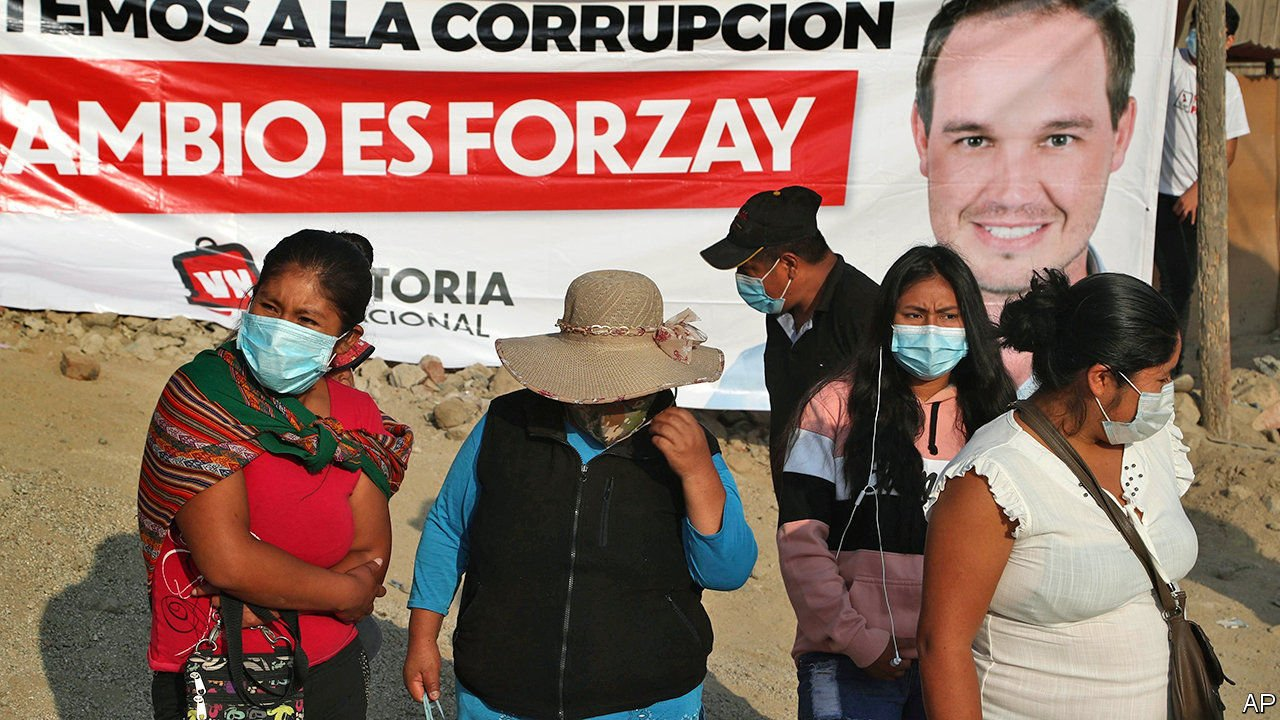
\includegraphics[width=0.8\textwidth]{images/20210327_amp501.jpg}
\end{figure*}
\lettrine{W}ITH LESS than three weeks to go before Peru's presidential election, opinion polls suggest a clear winner: a nihilist rejection of all 18 candidates. Add up the ``don't knows'' and those who tell pollsters they will cast blank or spoilt ballots and they come to around 30\%. But two people must go through to a run-off in June. Most of the candidates with a good shot of doing so are populists and outsiders, from both the left and right. 

Yonhy Lescano, a left-leaning populist and 20-year veteran of Congress, is the only candidate to poll in double digits (around a measly 13\%). Representing Popular Action, a long-established but amorphous party, he wants more state intervention in the economy and likes the look of places such as Bolivia (which have it). He promises greater oversight of businesses and to stop mining projects if they do not have support among the local population. 

Then there is Rafael López Aliaga: unknown until a few weeks ago, he now has 8\% in the polls and is rising fast. A businessman who is a member of Opus Dei, a conservative Roman Catholic movement, he boasts of his celibacy and of how he scourges himself. His critics see him as a Peruvian version of Brazil's Jair Bolsonaro (he denies this). He wants to cut red tape, reform social programmes and boot out a Brazilian construction firm, Odebrecht, which has been the subject of various corruption scandals. 

\begin{figure*}[h]
\centering
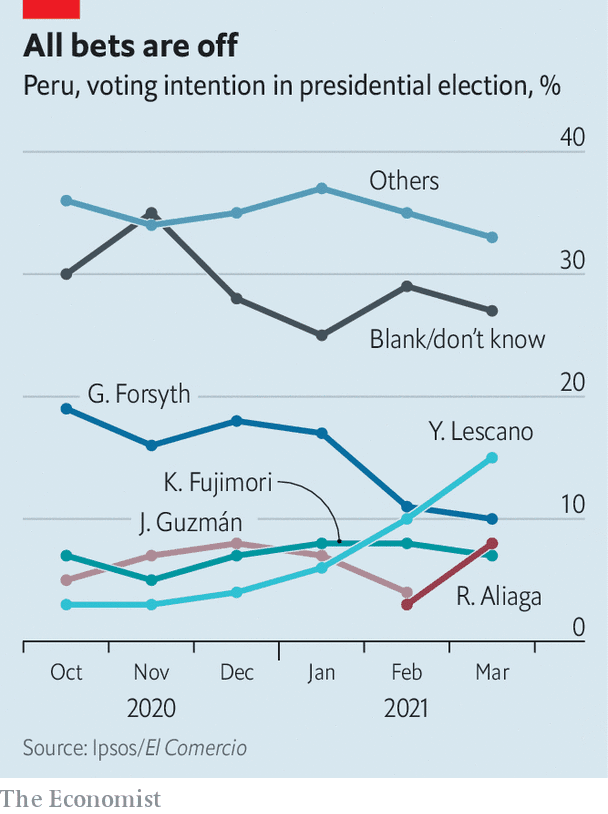
\includegraphics[width=0.4\textwidth]{images/20210327_amc288.png}
\end{figure*}


Another contender is George Forsyth, a former football goalkeeper and mayor, who has promised that, if he wins, he will be tough on crime. Having long led the opinion polls, Mr Forsyth's support has slipped recently. Opponents say his youth (he is 38) and inexperience render him ill-equipped for Peru's rough-and-tumble politics, which are more like rugby than soccer. Verónika Mendoza, a socialist, and Keiko Fujimori, a right-wing populist, also have a chance of making the run-off. 

Whoever wins will face a fractured Congress, also to be chosen on April 11th. Its 130 members could be split between as many as 11 parties. Since 2016 tensions between the executive and legislature have been a constant feature of political life and the country has had five presidents. 

Such a undistinguished crew of presidential candidates is nothing new. In 2011 Mario Vargas Llosa, a Nobel-prizewinning novelist, complained that in the elections that year Peruvians had a choice between ``AIDS and cancer''. Mr Vargas Llosa's gruesome quip was in reference to two candidates he felt would be particularly damaging---Ms Fujimori and Ollanta Humala, a former coup plotter who went on to win and who is also running again this year. 

The country is crying out for statesmanship it seems unlikely to get. It has been buffeted by the pandemic. Last year its economy shrank by 11\% and unemployment climbed to 13.8\%. Relative to its population of 33m, Peru has recorded more covid deaths than anywhere else in South America. As the title of one of Mr Vargas Llosa's recent novels declares, these are fierce times.{} 
\clearpage
\subsubsection{It was their backyard first }
\subsection{How a Canadian indigenous group could outwit NIMBYs }
\paragraph{Print Edition | The Americas  \quad \color{gray}{Mar 27th 2021 }}
\begin{figure*}[h]
\centering

\includegraphics[width=0.8\textwidth]{images/20210327_AMP004_0.jpg}
\end{figure*}
\lettrine{``I}T'S EASIER to elect a pope than to approve a small apartment building in the city of Vancouver,'' says Ginger Gosnell-Myers, of Nisga'a and Kwakwak'awakw heritage, and formerly the city's first-ever indigenous-relations manager. Such is the power of local NIMBYs that it is difficult to build new homes, and legions of young people are doomed to live with their parents for years, if not decades. But on some land the normal rules do not apply. No one can tell the Squamish First Nation, an indigenous group, what to build on their territory. 

One patch of its reserve is in Kitsilano, a ritzy part of Vancouver. Despite being close to the city centre, it is full of single-family homes and duplexes. Residents fiercely resist the construction of tall buildings. But they cannot stop the Squamish from erecting 59-storey skyscrapers. This year could see the ground broken for Senakw---12 towers containing 6,000 flats, mostly for renting. It would be the largest private indigenous development in Canada. 

Extra homes are sorely needed. Vancouver is the second-most-expensive city in the world, after Hong Kong. Tough zoning rules mean that the supply of new homes cannot meet demand. The Squamish, however, are free to build bigger, faster and cheaper than other landowners. Khelsilem (who goes by one name), the Squamish's spokesman, says a typical project of this size would spend five to ten years in the planning process. He expects Senakw to take two, provided the federal government responds quickly to the Squamish's request for a long lease on their land. Unlike other building projects, Senakw is not required to provide details to the public or hold town-hall meetings. 

The Squamish hope the project will bring in roughly C\$20bn (\$16bn) over 99 years. They could use the money. On average, Squamish people earn less and die earlier than other Canadians. The revenue from Senakw could be used for education and health care. 

If all goes to plan, Senakw could set a precedent. Urban reserve land is rare because indigenous people were pushed out of desirable areas by settlers in the 19th century. But a law passed in 2019 makes it easier to expand or create new reserves. That could lead to similar development opportunities for other indigenous groups. 

In 2019 the city vowed to put up 20,000 new rental units. Senakw would meet roughly a quarter of that target, points out Ms Gosnell-Myers. ``The Squamish Nation is more responsive to average Vancouverites than Vancouver city hall.''{} 
\clearpage
\subsubsection{Bello }
\subsection{Can Mercosur reverse decades of backsliding? }
\paragraph{Print Edition | The Americas  \quad \color{gray}{Mar 25th 2021 }}
\begin{figure*}[h]
\centering

\includegraphics[width=0.8\textwidth]{images/20210327_AMD001_0.jpg}
\end{figure*}
\lettrine{T}HIRTY YEARS ago South America had only recently emerged from dictatorships and protectionist isolation. It seemed like a revolutionary step when in 1991 the presidents of Argentina, Brazil, Paraguay and Uruguay sat down in Asunción and signed a treaty setting up a free-trade area that soon became Mercosur, a customs union of 200m people and a combined GDP of \$1trn. Coinciding with a wave of market-freeing reform, the philosophy behind it was known as open regionalism. ``With regional integration, we're going to be able to take part in world trade and world decision-making in the next century,'' Fernando Henrique Cardoso, then Brazil's president, told your columnist in 1996. 

Yet on March 26th, when the group's current presidents mark Mercosur's 30th birthday, there will not be much to celebrate beyond its mere survival. A first decade of rapid progress in integration was followed by two more of backsliding and protectionism. Trade within the bloc peaked as a share of its members' total trade at 25\% in 1997. Today that figure is just 14\%. True, the members' overall trade has expanded greatly, but most of that growth has been in exporting commodities to Asia. 

Mercosur has also struggled to stick to its own rules. Its common external tariff is littered with exceptions. Internal barriers are plentiful, too. The crudest was when Argentina's government encouraged protests against paper and pulp mills in Uruguay that blocked a key border bridge for years. 

There have been periodic efforts to revive Mercosur. The most recent involved trade-facilitation measures agreed on in 2017, with pro-business governments in Argentina and Brazil. Conscious of its isolation from global value-chains, Mercosur belatedly tried to reach trade agreements with the outside world. It now has zero-tariff agreements with all South American countries except the Guyanas. It is talking to several Asian countries. Most important, after 20 years of negotiations it struck a trade-and-co-operation agreement in 2019 with the European Union (EU). 

But Mercosur faces deep-rooted problems. They include macroeconomic volatility, as well as poor transport infrastructure. The biggest stumbling-block is political. No government is prepared to cede much sovereignty. Left and right, as currently represented by the governments of Argentina and Brazil respectively, often disagree radically about what regional integration means. Jair Bolsonaro's authoritarian but economically liberal government in Brazil wants to cut Mercosur's high external tariff; Alberto Fernández's leftist populist administration in Argentina, grappling with a deep slump, does not. They have few values in common. 

The 30th birthday party will be held online because of the pandemic (Mr Bolsonaro and Mr Fernández also dislike each other and have yet to meet in person). Uruguay will use the occasion to call for ``flexibility'' to negotiate its own trade agreements, a euphemism for Mercosur turning into a free-trade area rather than a customs union. That would involve changing the treaty, something neither Argentina or Brazil is likely to accept, thinks Rubens Barbosa, who was Brazil's first Mercosur co-ordinator. 

Mercosur's future will be defined by whether or not the EU agreement is ratified. Proponents see this as sealing a strategic alliance in a world of tensions between China and the United States. Mr Fernández's government is not enthusiastic. But it is Mr Bolsonaro who could be an insurmountable obstacle to ratification. The rampant deforestation in the Amazon, which has occurred on his watch, makes the agreement politically toxic in Europe, and gives an excuse to governments, such as France, which want to shield their farmers from Mercosur's more efficient ones. 

The European Commission is trying to draw up new rules on preventing deforestation to present to Mercosur. This is ``an attempt to keep the thing alive'', says Susana Malcorra, a former Argentine foreign minister. Realistically, conditions for ratification are unlikely until 2023, after elections in Germany, France and Brazil, and when Spain, a proponent, will hold the EU presidency. 

The agreement would bind Mercosur more tightly to its own rules. Without it, what would be the group's future? ``I don't think any of the countries will pay the political price of scrapping Mercosur,'' says Mr Barbosa. Instead, it would risk becoming another relic of Latin America's persistent failure to integrate, now for more than half a century. 
\clearpage
\section{Asia }
\subsubsection{From rags to stitches }
\subsection{As it turns 50, Bangladesh is doing well, despite its politicians }
\paragraph{Print Edition | Asia  \quad \color{gray}{Mar 25th 2021 }}
\begin{figure*}[h]
\centering

\includegraphics[width=0.8\textwidth]{images/20210327_ASP003_1.jpg}
\end{figure*}
\lettrine{I}N COLONIAL TIMES the eastern half of Bengal was one of the poorest parts of British India. After independence and partition in 1947, it became one of the poorest bits of Pakistan. And after it declared itself an independent country, Bangladesh, in 1971, it became poorer still, as the rump of Pakistan fought a savage war to retain it, destroying a big share of its few assets and killing many of its best and brightest. 

Few could have predicted how the tables would turn. This week marks 50 years since Bangladesh's first president, Sheikh Mujibur Rahman, declared independence on March 26th 1971. Over the intervening period the country's income per person has surpassed Pakistan's and is approaching India's (see left-hand chart). Before the pandemic, economic growth exceeded 7\% for four years in a row, outpacing not just Pakistan and India, but even China. 

Bangladeshis are not just vastly wealthier, but healthier and better educated too. Some 98\% of Bangladeshi children finish primary school, compared with less than a third during the 1980s. Literacy has soared (see right-hand chart). Infant mortality has plunged. Virtually everyone uses a toilet rather than defecating in the open. In all these respects, Bangladesh is doing better than both Pakistan and India. 

\begin{figure*}[h]
\centering
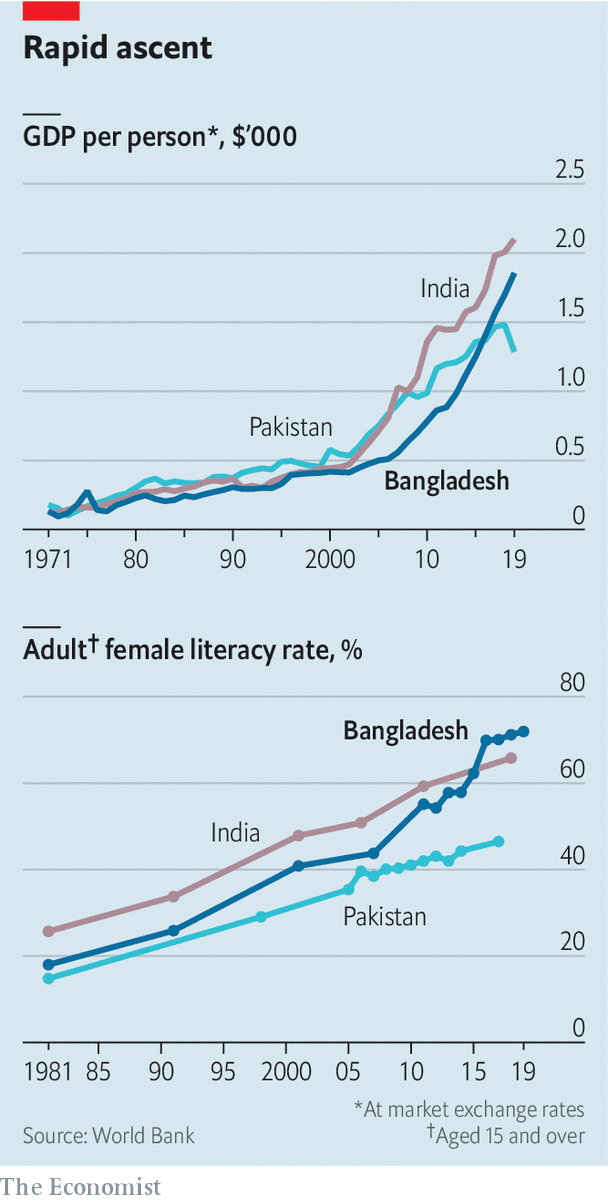
\includegraphics[width=0.4\textwidth]{images/20210327_ASC297_0.png}
\end{figure*}


Devastating as the war of independence was, in some ways it set Bangladesh on the path to success. Many expatriates came home to help their new country recover. Zafarullah Chowdhury, who dropped out of university in Britain, set up a charity that helped to distribute cheap generic drugs and contraceptives. Fazle Hasan Abed sold his flat in London to return before founding another charity, BRAC, that taught mothers how to rehydrate children suffering from diarrhoea, turning it from a deadly illness to a nuisance. 

The overstretched government was only too happy to allow aid agencies and NGOs to take on such tasks. In a drive in the 1980s to vaccinate children against diseases like polio, the country was split down the middle: the government took one half, BRAC the other. By the end of the decade the immunisation rate had risen from 2\% to 80\%. 

Charities like BRAC had an especially big impact because they targeted women. By the 1990s it was running 64,000 schools, which were not only educating girls but employing women to teach in them. There are now more girls in high school than boys (another difference from India and Pakistan). BRAC and other organisations also popularised microcredit, turning millions of rural women into entrepreneurs. 

Bangladesh's booming garment industry has helped to improve women's welfare, too, argues Rubana Huq of the Bangladesh Garment Manufacturers and Exporters Association. The share of women in paid work has risen from 3\% 50 years ago to 36\% today. Some 80\% of Bangladesh's 4m garment workers are women. Their work ``earns them economic freedom and dignity at home and outside'', says Ms Huq. 

The garment industry has become the world's second largest, accounting for 11\% of GDP and 80\% of export revenue. Successive governments have helped mainly by getting out of the way, simplifying labour laws and removing import duties on inputs. This free-market approach was crucial in fomenting growth, says Fahmida Khatun of the Centre for Policy Dialogue, a think-tank in Dhaka. 

Yet Bangladesh's politics is as depressing as its development is uplifting. Sheikh Mujib tried to turn the country into a one-party state, but was quickly assassinated. The current prime minister, his daughter, Sheikh Hasina Wazed, seems determined to make his vision a reality. Since coming to power for a second time in 2009, she has abolished the practice of holding elections under an impartial caretaker government. The main opposition figure, Khaleda Zia, was arrested in 2015. She has since been convicted of corruption and banned from politics in a trial she says was politically motivated. Before the most recent election, in 2018, opposition parties claimed that more than 7,000 of their activists had been arrested. Many opposition candidates, like Ms Zia, were barred from running owing to criminal convictions. Sheikh Hasina's Awami League and its allies won 288 of 300 seats. 

It is not just opposition activists, but also journalists and other critics of the government who increasingly wind up behind bars. In 2018 the government introduced the Digital Security Act, supposedly to curb religious radicalism and pornography online. But its vague provisions, which include stiff jail sentences for those who post ``aggressive or frightening'' content, have been used to silence critics of all sorts. Mushtaq Ahmed, a writer, was arrested last year after criticising the government's response to covid-19 on Facebook. He died in prison last month, having been denied bail six times. 

Members of the Awami League, meanwhile, easily secure bail for serious crimes, if they are charged at all. Government contracts often go to the party's cronies. State-owned banks are weighed down by loans that well-connected borrowers decline to repay. There is no point going to court: the party with the closer ties to the Awami League always wins. ``We literally don't have breach of contract cases anymore,'' explains Shahdeen Malik, a lawyer who argues cases before the Supreme Court. The tax code, which relies more on levies on consumption than on income or wealth, is also skewed in favour of the rich and politically connected. 

The iniquities of this system are beginning to be reflected in the economic data. Between 2010 and 2016 the richest\textbf{}households saw their income rise by nearly a quarter, while the poorest households saw theirs decline by a third. Zahid Hussain, a former lead economist on Bangladesh for the World Bank, blames the rent-seeking behaviour of the elite. Corruption knocks two percentage points off GDP growth each year, the bank has estimated. At any rate, foreign investment has stagnated, perhaps owing in part to the caprice of the courts. 

Covid-19 has exacerbated inequality by pushing millions who had escaped poverty back into it. The proportion of Bangladeshis living below the national poverty line has risen from around a quarter to 40\% or so, says Asif Saleh, the head of BRAC. No one is able to travel abroad for work anymore, which bodes ill for future flows of remittances. These reached almost \$20bn last year. Garment factories have been battered by cancellations, as lockdowns abroad have crimped sales of clothing. 

\begin{figure*}[h]
\centering
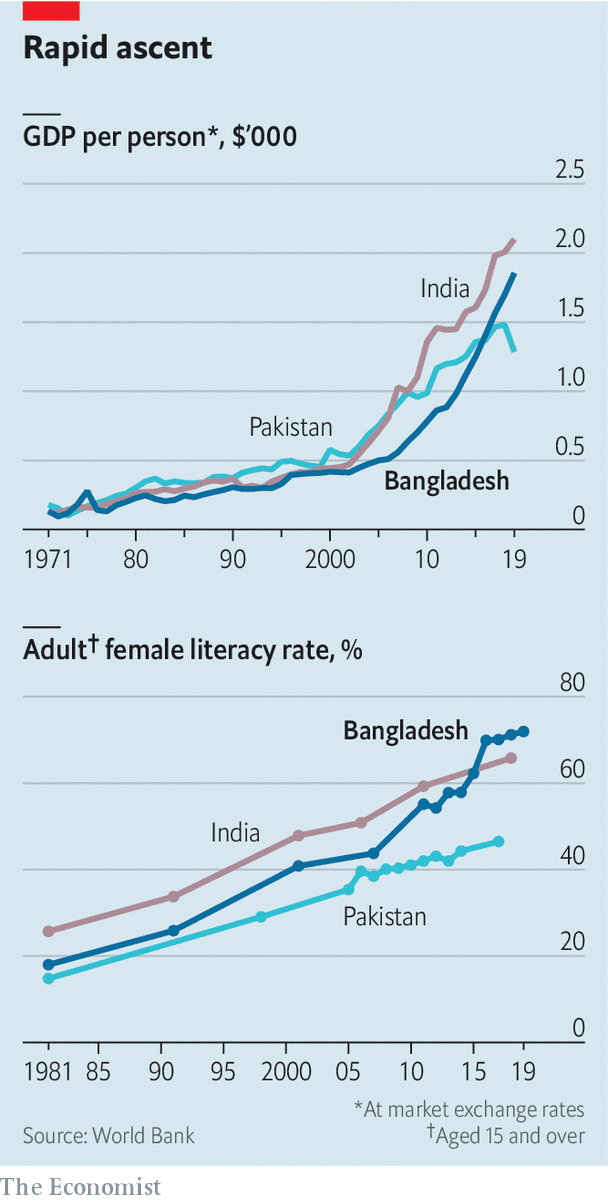
\includegraphics[width=0.4\textwidth]{images/20210327_ASC297_0.png}
\end{figure*}


The increase in women's participation in the workforce has slowed, notes Ms Huq. Between 2005 and 2010\textbf{}it grew by 1.7 percentage points a year on average, but since then by only 0.7 percentage points a year. She thinks women's rights are in retreat, too. Without the rule of law or political accountability, violence against women goes unchecked, she argues. 

By centralising power in herself, Sheikh Hasina has also added an element of political uncertainty. As tight as her grip on her country is, it cannot endure past the grave. She is 73, but has no clear successor. Relatives and other close allies appear to be jockeying for position. Her son, Sajeeb Wazed, is an adviser to the government. His sister, Saima Wazed, who had been living in Canada, has recently been given a number of government jobs, prompting speculation that she is being groomed for power. Other contenders include their cousin, Radwan Mujib Siddiq Bobby, who has begun publishing a magazine about public policy, and Sheikh Fazle Noor Taposh, the mayor of South Dhaka. His parents were assassinated along with Sheikh Hasina's in 1975. None of them has the same venerable status as Sheikh Hasina, however, and none is a plausible reformer. 

Some speculate that change may come from the army, which has seized control several times in the past. But Sheikh Hasina has a tight grip on it, too. Al-Jazeera, a broadcaster based in Qatar, recently exposed the close personal ties between Sheikh Hasina and the current army chief. 

Others fear Islamic radicalism. In 2016 religious extremists killed 24 people at a restaurant and bakery in Dhaka. Sheikh Hasina has cracked down on some Islamist groups, cajoling the courts to ban a prominent Islamic party, Jamaat-e-Islami, which fought alongside Pakistan in the war of independence. But she has cosied up to others, including Hefazat-e-Islam, which has agitated against the secularism for which the Awami League theoretically stands. Ordinary Bangladeshis, some 90\% of whom are Muslim, have grown more religiously observant in recent years, but few seem to hanker for a theocracy. 

Indeed, so complete has the Awami League's control become that it is hard to know what ordinary Bangladeshis do want. Most will presumably be content if their personal welfare improves in the future as rapidly as it has done over the past 50 years. That happened largely in spite of Bangladesh's politicians, however, not thanks to them. {} 
\clearpage
\subsubsection{Purple pose }
\subsection{A rural bit of South Korea tries to become a tourism hotspot }
\paragraph{Print Edition | Asia  \quad \color{gray}{Mar 25th 2021 }}
\begin{figure*}[h]
\centering
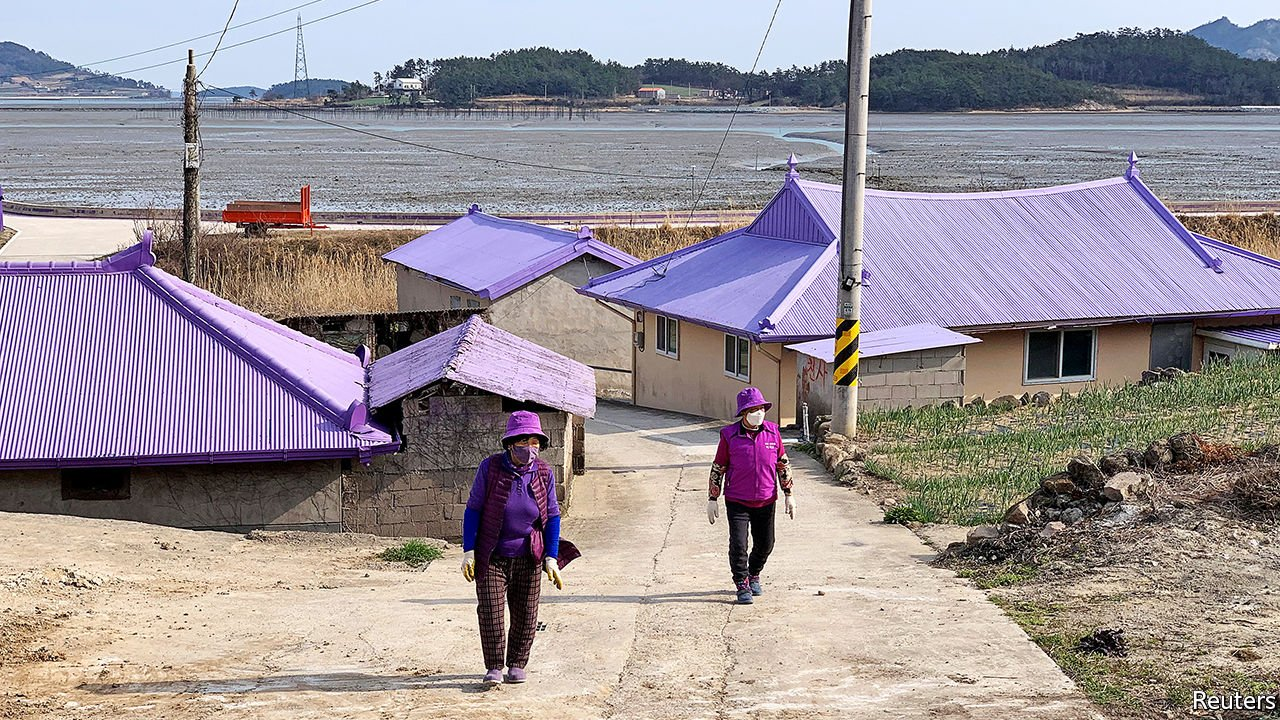
\includegraphics[width=0.8\textwidth]{images/20210327_ASP001_0.jpg}
\end{figure*}
\lettrine{T}HE ISLANDS of Sinan county, off South Korea's south-western coast, have never been a centre of anything much. Sustained by fishing, seaweed harvesting and salt farming, most are sparsely populated or entirely uninhabited. Reaching Mokpo, the nearest city, requires choppy ferry rides or slow car journeys along winding roads and across enormous bridges. As in most rural areas of South Korea, the local population is shrinking and ageing fast---and economic opportunities have been atrophying with it. 

A few years ago the region briefly became notorious when it was revealed that workers on the salt farms were being treated like slaves, with the connivance of local officials. Police officers from Seoul trusted their local counterparts so little that they travelled to the area undercover to investigate. One of the outcomes of the scandal was supposed to be the construction of a new police station, but seven years on there is only an empty lot with a tattered purple sign reading, ``Sinan police''. 

The colour is no accident. Officials are trying to rebrand Sinan as a tourist destination with a purple theme. Two nearby islands, Banwoldo and Bakjido, have been transformed into an Instagram-ready curiosity through the application of lots of purple paint. Shops and houses have purple roofs and facades. The islands are connected by a purple walkway; purple paths are lined by purple flowers. A worker from the tourism association tending the flowers wears a purple hat. 

At one level the scheme, cooked up in 2015 by Lee Nak-yeon, the provincial governor at the time, has been a resounding success. It has attracted nearly half a million additional visitors to the region since the spring of 2019, when the completion of a bridge made it possible to drive rather than take the ferry to the purple islands. Petrol-station attendants and coffee-shop owners along the route from Mokpo report a welcome surge in business that has been sustained even during the pandemic. Kim Ae-ran, a 70-something chicken farmer in a lilac face mask who runs a (purple) co-operative shop for local produce on the islands, says it is doing well: ``It's all very healthy and organic, city people love that.'' 

But not all locals are equally enthusiastic. ``I don't like it at all,'' says one elderly resident working in her (white) cabbage patch not far from the purple path. ``All the tourists bring is rubbish, and purple? Of all the colours they could have chosen! But what could I do when they offered to fix my roof free of charge?'' Kim Hyun-kyung, the tourism-office worker in the purple hat, acknowledges that some residents were initially miffed: ``But we fixed their houses and improved the roads, so most of them have come to terms with it.'' 

If the purple islands have inspired mixed feelings, other official development efforts have provoked more serious opposition. In February Moon Jae-in, the president, travelled to Jido in northern Sinan to announce that the mudflats off the coast would soon host the country's largest offshore wind farm. The \$40bn project is supposed to create 120,000 new jobs in the region. The president made the announcement on a new bridge connecting three of the islands. If the project goes ahead as planned, the coming decade will see yet more city slickers roll up in Sinan, albeit with hardhats instead of cameras. 

Not all locals are pleased. When plans for the wind farm were first floated four years ago, fishermen and seaweed-farmers staged fierce protests, fearing it would disrupt their work. At the port below the bridge on which Mr Moon made his speech last month, shop owners and local residents are united in their opposition to both the wind farm and the bridge. ``I heard the wind farm will scare away all the fish,'' says a 78-year-old woman waiting for the ferry. ``All the fishermen tried to stop it but I guess the president has been here now so it'll happen.'' ``Nobody will come down to the port any more now the bridge is built, I might as well jump off it,'' says a 60-something woman running a convenience store. ``We all saw his motorcade when he came. He could at least have acknowledged we were here.'' {} 
\clearpage
\subsubsection{Stack 'em high }
\subsection{Cambodia's strongman is trying opposition politicians en masse }
\paragraph{Print Edition | Asia  \quad \color{gray}{Mar 25th 2021 }}
\begin{figure*}[h]
\centering
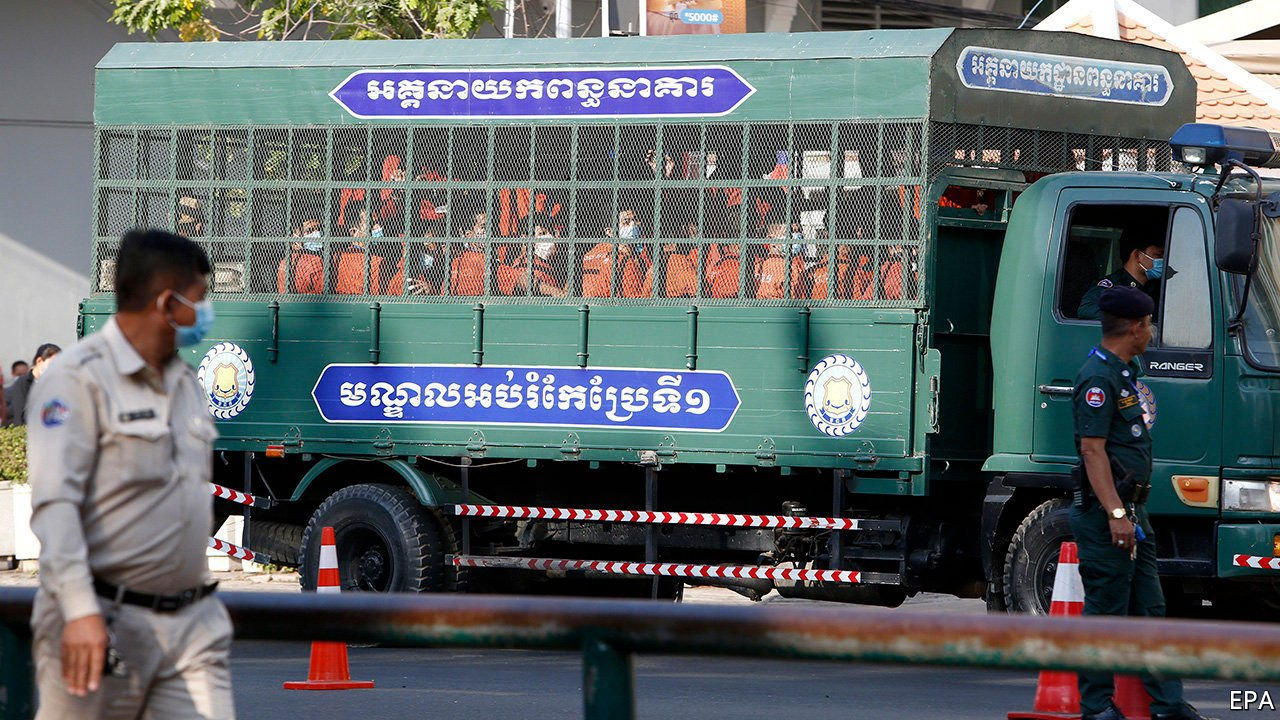
\includegraphics[width=0.8\textwidth]{images/20210327_asp501.jpg}
\end{figure*}
\lettrine{I}T IS DIFFICULT for anyone to argue that Sam Rainsy, Cambodia's leading opposition figure, is not guilty of the crimes for which he was sentenced on March 1st to 25 years in prison. That is because the charges were so nebulous as to encompass almost everything an opposition politician does. He was accused of attacking the country's institutions, and encouraging others to do the same. 

It is even harder for Mr Sam Rainsy to defend himself in person, since the government will not let him into the country. The prime minister, he explains, has threatened to shoot down any plane bringing him home from exile in France, ``meaning I was not welcome''. 

At the same trial, the municipal court in Phnom Penh, the capital, sentenced eight other senior members of the banned Cambodian National Rescue Party (CNRP), all of whom were absent, to between 20 and 22 years' imprisonment. Some 150 lower-ranking members of the party are still on trial. To make the mass hearings more manageable, the defendants have been clumped into three different groups, of roughly 20, 60 and 70. Nobody is quite sure of the exact numbers. Chak Sopheap of the Cambodian Centre for Human Rights, a pressure group, calls it the ``political instrumentalisation of the justice system''. Another observer describes it as ``rule by law'' rather than ``rule of law''. 

After the CNRP nearly unseated the ruling Cambodian People's Party in national elections in 2013, Hun Sen, Cambodia's strongman since 1985, set about dismantling it methodically. First he had the Supreme Court ban the party outright in 2017. After that the authorities began hounding its members. Even low-ranking activists in the provinces have been threatened or hauled into court. ``People are really intimidated,'' says Mr Sam Rainsy. ``If they demonstrate they are met with violence. And if they continue they will be arrested.'' 

Yet one trial, against Kem Sokha, who founded the CNRP with Mr Sam Rainsy, is proceeding oddly slowly. Like other leaders of the party, he was barred from politics for five years when it was banned in 2017. But the authorities suspended a different case against him last year, ostensibly because of the dangers of holding hearings amid the pandemic. (Confusingly, the mass trials do not seem to worry anyone in that respect.) While he waits for the proceedings to resume, the courts have freed him from house arrest. 

Most observers interpret all this as a transparent attempt to divide the opposition. The \emph{Khmer Times}, a government mouthpiece, gleefully noted recently that supporters of the two founders ``are becoming increasingly divided''. 

Mr Hun Sen may be hoping to lure a faction of the CNRP to participate in municipal elections next year. The most recent general election, in 2018, at which the ruling party won 125 out of the 125 seats in the national assembly, was slightly embarrassing. The participation of some genuine opposition figures might help the next look like less of a sham. 

But the European Union, at least, does not appear to have been fooled. On March 11th the European Parliament said it was ``appalled'' by human-right violations in Cambodia. Last year the EU imposed tariffs on about 20\% of imports from Cambodia in protest at the government's repression. Mr Sam Rainsy thinks more targeted measures are needed. The elite park their money, send their children to study and take agreeable holidays in the West, he says. ``If measures affect their personal interest, they will react.'' {} 
\clearpage
\subsubsection{The Kolkata clan }
\subsection{While India and China bicker, ethnic-Chinese Indians move away }
\paragraph{Print Edition | Asia  \quad \color{gray}{Mar 25th 2021 }}
\begin{figure*}[h]
\centering
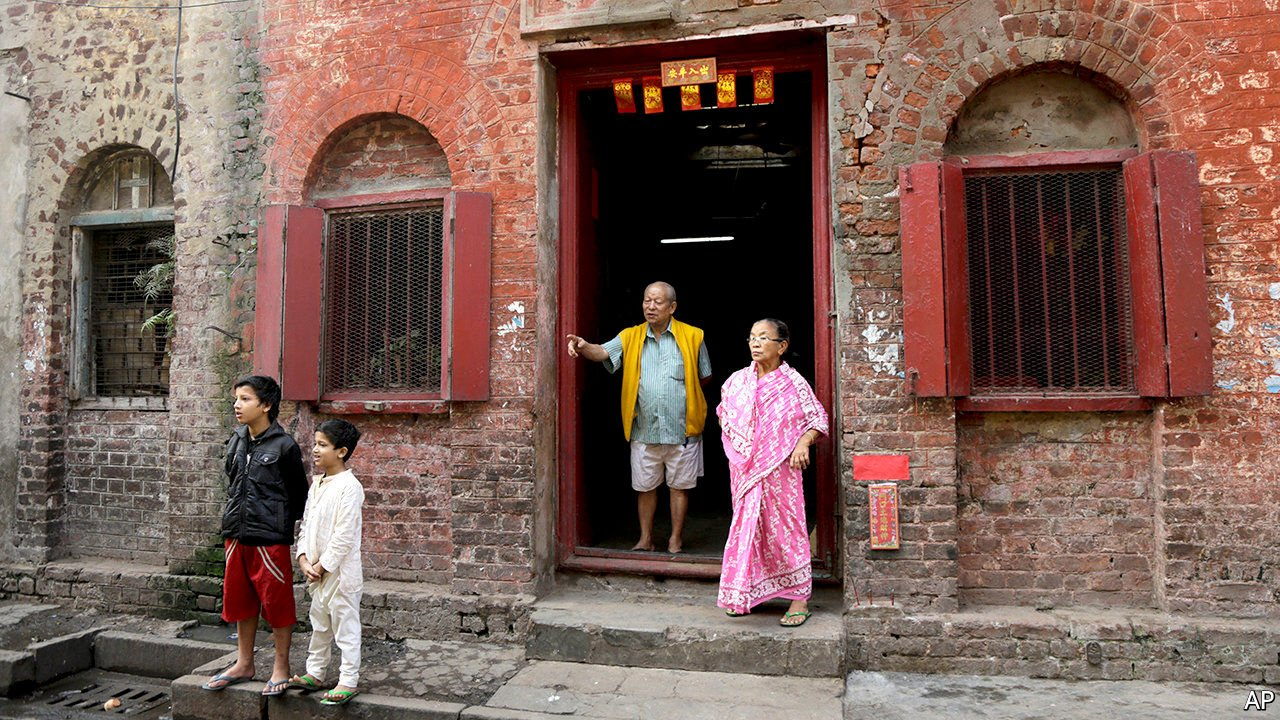
\includegraphics[width=0.8\textwidth]{images/20210327_asp502.jpg}
\end{figure*}
\lettrine{T}HE SUNFLOWER beauty salon on Russel Street in Kolkata has been gutted for renovation, but a row of elegant Indian ladies sits perched inside its temporary digs, an air-conditioned cargo container. The hairdressers, sisters-in-law named Winnie and Patsy, snip away while chatting to their clients in Hindi, Bengali and English---and to each other in Hakka, a language of southern China. Prettified heads can look through makeshift windows at signs in Chinese across the street, which announce the Shanghai Company, a laundry in an art-deco pile from the 1930s. At the street corner a club offers a Chinese \emph{thali}, a form of trans-Himalayan fusion cuisine. In the city's two Chinatowns red lanterns herald Taoist temples and clan associations. 

Kolkata has long been home to India's largest Chinese community. At its peak, when Calcutta (as it then was) was the capital of imperial India, it was home to 50,000 ethnic Chinese. But relations between the two Asian giants are often testy. In 1962, when they fought a brief border war, about 15,000 Chinese from Kolkata were rounded up. Thousands were interned in prison camps in the desert in far-off Rajasthan. When they made their way back home, they found the government had auctioned off their property. Winnie lost her father and her chance of schooling, but managed to open her salon in 1968. 

Indian and Chinese forces have been fighting along the Himalayan border again over the past year, in the worst clashes since the 1960s. On June 15th 20 Indian soldiers were beaten to death. In response nationalist groups called for a boycott of Chinese goods and even of Chinese food (although that is invariably cooked by Indians). The national government banned a series of popular Chinese-owned mobile-phone apps. The \emph{Global Times}, a belligerent state-run newspaper in China, reported a ``wave of anti-China sentiment in India''. 

Few residents of Kolkata have turned on their ethnic-Chinese compatriots, however. To show where their loyalties lay, a group of Chinese-Kolkatans organised a sing-along of a patriotic Indian songs. Chinese temples flew the Indian tricolour, as usual. Older locals still favour Chinese carpenters, dentists and cobblers. 

Yet the Chinese community is wilting, anyway. It now numbers perhaps 2,500. Many more ``Calcutta Chinese'' live in Markham, a city in Canada, than in Kolkata. At the Sunflower, Winnie's niece gossips at the till about Canadian visas. 

Patrick Lee wishes any of his children would come back from abroad to keep his family's business going. He and his brothers make eco-friendly leather and bottle spicy sauce for the Pou Chong brand. India, he feels, has been a good home to his family, though his in-laws were incarcerated in 1962. ``Overnight they lost everything, entire life's earnings, everything. So there is some fear.'' {} 
\clearpage
\subsubsection{Downgrading Delhi }
\subsection{India's ruling party finds a new way to hamstring the opposition }
\paragraph{Print Edition | Asia  \quad \color{gray}{Mar 25th 2021 }}
\begin{figure*}[h]
\centering
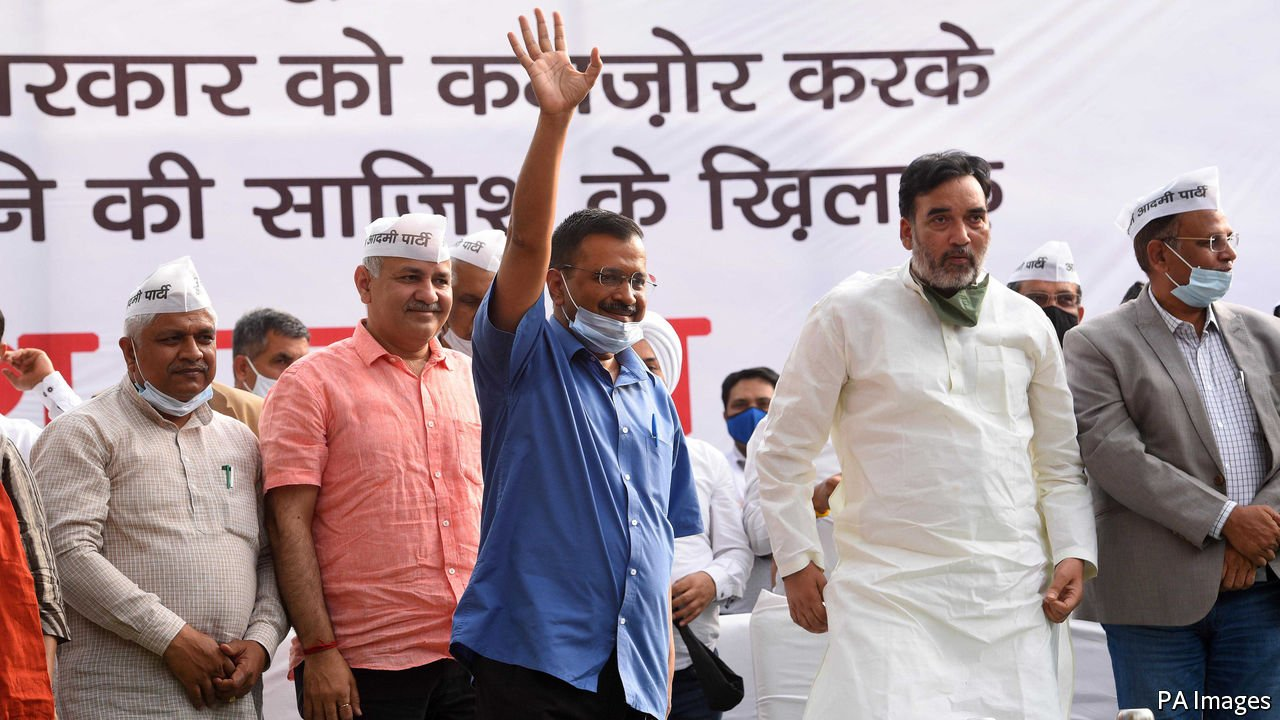
\includegraphics[width=0.8\textwidth]{images/20210327_asp503.jpg}
\end{figure*}
\lettrine{W}HEN NARENDRA MODI, India's prime minister, stripped Kashmir of its statehood in 2019, most Indians cheered. The Muslim-majority territory had long been troublesome. The triumphal consensus was that Kashmir's special autonomy, which Mr Modi abolished using all kinds of constitutional tricks, had only encouraged ``anti-national'' attitudes, and that Kashmir had got what it deserved. 

Pratap Bhanu Mehta, an academic and columnist for the \emph{Indian Express}, a national newspaper, was one of the few to raise misgivings. A government that gleefully twisted the law and suspended local democracy in one place could surely do the same in another. Mr Modi proposed to ``Indianise'' Kashmir, noted Mr Mehta. ``Instead, what we will see is potentially the Kashmirisation of India.'' 

Sooner and closer to home than anyone expected, Mr Mehta's prediction has come to pass. On March 22nd Mr Modi's Bharatiya Janata Party (BJP) rushed a bill through the lower house of parliament to strip the elected government of Delhi, the capital, of much of its power and hand this instead to the lieutenant-governor, an official who represents the central government. It won the approval of the upper house on March 24th. It is as if the state of New York, the population of which is similar to Delhi's, were suddenly to be placed under the authority not of its legislature or elected governor, but of a bureaucrat appointed by a hostile Congress. 

Even before Mr Modi's power-grab, the administration of Delhi was convoluted. Formally it is one of India's eight ``union territories'', not one of its 28 fully fledged states. Yet since independence in 1947 the city had gained increasing powers of self-rule, including its own legislature and chief minister. In 2018 the Supreme Court further limited the role of the lieutenant-governor, affirming the primacy of the locally elected government. 

The new law adds to the contortions, but its intent is clear. ``All executive action'', it says, must now be approved by the lieutenant-governor. The city's legislature may no longer ``consider matters of day-to-day administration'' or inquire into administrative decisions. All rules or inquiries ever made by the body are retroactively void. 

There are multiple ironies in this affront to democracy. One is that for decades the BJP itself has noisily demanded full statehood for Delhi. Another is that Arvind Kejriwal, leader of the opposition Aam Aadmi party and the city's chief minister since 2015, loudly praised Mr Modi's usurpation in Kashmir. He is now paying a price not only for repeatedly beating the BJP in elections in Delhi, but also for having the temerity to support protesting farmers and to try to build a following in Mr Modi's home state of Gujarat, among other places. 

It does not help that among other inquiries, Delhi's legislature has probed the sectarian riots in the city that left 53 people dead last year, mostly Muslims. The police, under the control of the central government, have painted an Islamist conspiracy as the cause, but glaring evidence points instead to incitement by Hindu nationalists, including stalwarts of the BJP. 

Mr Kejriwal's demotion serves as a blunt warning to those who stand in the BJP's way. Under Mr Modi the party has not merely won thumping majorities in two national elections, but also powered to victory in state elections across the country. In states where it has lost elections, it has repeatedly taken control by persuading legislators to defect from other parties. The downgrading of local governments in Kashmir and now Delhi marks a third route to power. 

What does Mr Mehta, the lonely voice over Kashmir, say now? Earlier this month he resigned from Ashoka University, a private institution on the outskirts of Delhi. ``My public writing in support of a politics that tries to honour constitutional values of freedom and equal respect for all citizens is perceived to carry risks for the university,'' he said in his resignation letter. It is not just nettlesome politicians that the BJP finds ways to sideline. {} 
\clearpage
\subsubsection{Banyan }
\subsection{India and China are finding vaccine diplomacy tricky }
\paragraph{Print Edition | Asia  \quad \color{gray}{Mar 27th 2021 }}
\begin{figure*}[h]
\centering

\includegraphics[width=0.8\textwidth]{images/20210327_ASD001_0.jpg}
\end{figure*}
\lettrine{A} YEAR AFTER China barred entry to most foreigners as the covid-19 pandemic spread, its embassies in India and a score of other countries have just declared that they will make it easier for expatriates who had been living in China to return. They must be vaccinated first. But there is a bigger catch: only those who have received made-in-China shots need apply. India, for one, has not approved the use of any Chinese vaccine. 

It is something of a public-relations own goal---a reminder of how the altruism that China's ``vaccine diplomacy'' is intended to showcase is often undermined by grubbier calculations and missteps. Months ago China recognised that rich countries would be too busy getting their own populations jabbed to give serious thought to poorer places. China could both earn gratitude and present itself as a scientific, diplomatic and even moral powerhouse. More cynically, vaccine diplomacy was a tool to rewrite history: to change the narrative of China as the source of the plague to the world's saviour from it. 

Urged on by President Xi Jinping, the state pumped money into vaccine development and signed deals with dozens of countries. With vaccines that its leaders claimed would be cheaper and easier to store than those being developed in the West, China would change the course of the pandemic. The two leading producers, Sinovac and Sinopharm, claimed to be able to produce 2bn doses a year between them. 

Yet China's vaccine diplomacy has stumbled, and not only because of delayed production and shipment. China's eagerness for countries to take its vaccines is matched by its reluctance to share the data from clinical trials. That is presumably because Chinese vaccines are less effective than Western ones. It all erodes trust. Singapore paid for the option of the Sinovac shot, among several ordered from around the world. Yet China ``blew it'', in the words of an insider, when its embassy trumpeted the arrival of a Sinovac consignment last month before the Singaporean government had approved the drug. It will not do that without the data China declines to provide. 

The Philippine government, which threw in its lot with China when coronavirus vaccinations began in March, is struggling to persuade a population badly hit by the pandemic to accept Chinese jabs. A scandal concerning a black market for unregulated shots, aimed mainly at Chinese workers, has not helped. Nor has the recent discovery of 200 Chinese vessels occupying a reef within what the Philippines considers its territorial waters. China, says Ronald Mendoza of Ateneo de Manila University, is not doing well at winning hearts and minds. 

China has not blown it everywhere. A Chinese shot in the arm is surely much better than none at all. And countries such as Indonesia and Malaysia, which did not secure enough Western vaccines, are glad of Chinese help. Yet China is not the only Asian country capable of mass-producing vaccines and hoping to generate goodwill as a consequence. India is a vaccine giant, sitting at the heart of medical supply chains. Its manufacturers already play a big role in the production of AstraZeneca's vaccine against covid-19. Russia depends on India for the global roll-out of its Sputnik vaccine. 

India has been ramping up shipments to neighbours such as Bangladesh, Nepal and Sri Lanka. In fact, it has exported more doses (60m) than it has used at home (44m). In theory, its vaccine diplomacy was turbocharged at a recent virtual summit of the ``Quad'' grouping of Australia, India, Japan and the United States. The foursome agreed to fund the production of 1bn Indian-made vaccines for distribution to countries in need by the end of 2022. 

Yet even more than China, India faces a tension between vaccinating its own vast population and helping other countries. A suffocatingly statist approach that initially excluded the private sector meant a slow start to its own vaccination programme, especially among the poor. This week it froze all exports of the AstraZeneca vaccine to ensure bigger supplies at home, amid a surging second wave of infections---an own goal of its own. 

Shivshankar Menon, a former Indian foreign secretary, doubts that efforts at vaccine diplomacy alone, even when deftly handled, will do much to increase either China or India's influence or standing. People see through claims of altruism, he says. But at least the Quad reflects an effort to do something for the global good---a collective response that has been all too rare in this pandemic. 
\clearpage
\section{China }
\subsubsection{Winter of discontent }
\subsection{Will countries boycott China's Olympics in 2022? }
\paragraph{Print Edition | China  \quad \color{gray}{Mar 27th 2021 }}
\begin{figure*}[h]
\centering
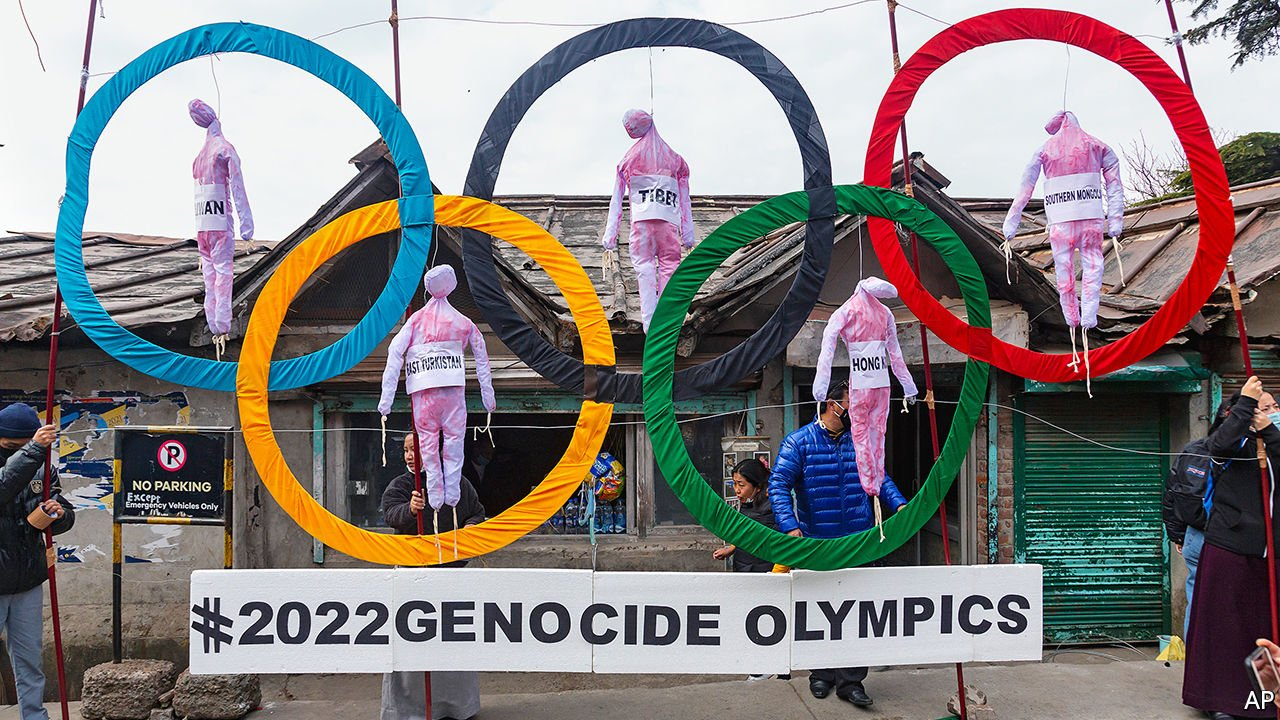
\includegraphics[width=0.8\textwidth]{images/20210327_CNP001_0.jpg}
\end{figure*}
\lettrine{I}N 2015, WHEN the International Olympic Committee (IOC) awarded the 2022 Winter Olympics to Beijing, some people criticised the decision because of China's human-rights record. Just in the previous few weeks China had rounded up hundreds of civil-society activists across the country. But the rival candidate for the games was another authoritarian state, Kazakhstan. Democracies such as Norway had pulled out of the race. And few people even imagined that, within two years, China would be building a gulag in Xinjiang to incarcerate more than 1m ethnic Uyghurs because of their religious and cultural beliefs. 

Attitudes in the West towards China have hardened a lot since the IOC made its decision. In January America called the repression in Xinjiang ``genocide''. On March 22nd it joined Britain, Canada and the European Union in a simultaneous declaration of sanctions against Chinese officials involved in that region's atrocities. It was a rare co-ordinated attempt by Western powers to put pressure on China over its human-rights record. They have been riled, too, by China's clampdown in Hong Kong and its growing challenge to liberal norms globally. The winter games, which are due to begin on February 4th, will be among the most controversial in Olympic history. 

So far no country appears likely to refuse to send athletes, as America did in 1980 when it boycotted the summer Olympics in Moscow in protest against the Soviet Union's invasion of Afghanistan. (Eastern Bloc countries in turn boycotted the 1984 summer games in Los Angeles.) Nor are the games expected to be moved somewhere else, despite calls for such action by activists and some politicians in America, Canada and Europe. The IOC says the games are about sport, not politics, and will go ahead. Corporate sponsors, too, have not budged in their support. But as the games draw nearer, calls will grow for boycotts of various kinds. In 2008, when Beijing hosted the summer games, some activists labelled that event the ``genocide Olympics'' because of China's support for Sudan, then conducting mass killings in Darfur. This time, although the horrors in Xinjiang do not involve slaughter, the label is more likely to stick (Tibetan protesters in India are pictured). 

Some countries' leaders may stay away, as may some athletes. America's president, Joe Biden, has yet to clarify what he will do. But it is unlikely that he or any other senior American official will attend, given how they have described China's actions in Xinjiang. Mitt Romney, a Republican senator, wrote this month that his country should send its athletes but ask spectators, other than participants' family members, not to go. China may decide to keep tight border-controls anyway, if it fears a resurgence of covid-19. On March 20th Japan said spectators from abroad would be barred from the Tokyo Olympics, which begin in July, because of the pandemic. 

Companies that are sponsoring the games will face growing pressure. Zumretay Arkin of the World Uyghur Congress, a group based in Germany, says she and other activists are approaching these firms ``one by one'' and will, if necessary, ``publicly name and shame'' them. The campaigners have started with Airbnb, an American home-rental firm. It is one of the IOC's main Olympic sponsors, which also include Coca-Cola, Samsung and Visa. Airbnb signed its sponsorship deal in November 2019, when the new gulag in Xinjiang was already well-known. 

On March 23rd more than 190 groups representing Tibetan, Uyghur and other China-related causes issued a public letter to Brian Chesky, Airbnb's boss. It called on him to withdraw his firm's sponsorship or ``risk being tainted'' by association with the games. Contacted by \emph{The Economist}, Airbnb did not respond specifically to the letter or comment on the Olympics. A spokeswoman referred to a statement, issued by the firm in January, that acknowledged some Airbnb hosts in China had violated company policy by rejecting ethnic-minority customers. The statement said rental listings that appeared discriminatory would be removed. 

A similar letter has been sent to Grant Reid, the chief executive of Mars Wrigley, which will also soon be published. In December 2019 the sweetmaker reached a deal with Beijing's Olympic committee that Snickers, a peanut-filled Mars Wrigley product, would be the ``official chocolate'' of the games. The firm did not respond to a request for comment. Executives at Coca-Cola and Visa who work on social-responsibility issues also did not reply when invited to discuss their firms' Olympic deals. 

On March 18th Ms Arkin of the World Uyghur Congress, along with campaigners for human rights in Tibet, held a virtual meeting with IOC officials to raise their concerns. In 2015 the IOC had told such activists that it had received ``assurances'' from Chinese officials during the bidding process regarding human rights, and that it was confident the Olympic charter would be respected. (The charter promotes ``respect for universal fundamental ethical principles'' and the ``preservation of human dignity''.) But IOC officials were cautious in their comments on human-rights abuses in China when it staged the Olympics in 2008, despite a brutal security clampdown on unrest in Tibet that year. 

IOC officials say boycotts punish athletes and do not work: the Soviet occupation of Afghanistan continued for eight years after the Moscow Olympics. The IOC shunned South Africa during the apartheid era, but notes that it did so in concert with a broad UN-backed international movement. South Africa, however, lacked the political and economic might of China. This month Thomas Bach, the IOC's president, said his organisation was not a ``super world government''. 

Activists fear a repeat of 2008, when China used the games to show off its metaphorical muscles. Thousands of Chinese troops performed in the opening ceremony, which also included children carrying the Chinese flag while dressed in traditional costumes representing Tibet and China's other ethnic minorities. It was a coming-out party for a rising great power. 

But in its newfound confidence, China has made new enemies. If Michael Kovrig and Michael Spavor, two Canadians arrested in China in response to the detention in Canada of a Huawei executive, remain in custody, there will be anger not least in Canada, a Winter Olympic superpower. (In recent days ``the two Michaels'' have appeared in court for one-day trials, after more than two years in prison.) If China maintains its economic pressure on Australia, calls may grow in that country for a boycott. In Europe, officials are angry about sanctions imposed by China on March 22nd against lawmakers and academics in response to the EU's Xinjiang sanctions. If an Olympic boycott movement gains momentum, it may be due as much to China's behaviour abroad as to its abuses at home. {} 
\clearpage
\subsubsection{No silver lining }
\subsection{Cloud-seeding will not solve China's water shortages }
\paragraph{Print Edition | China  \quad \color{gray}{Mar 27th 2021 }}
\begin{figure*}[h]
\centering
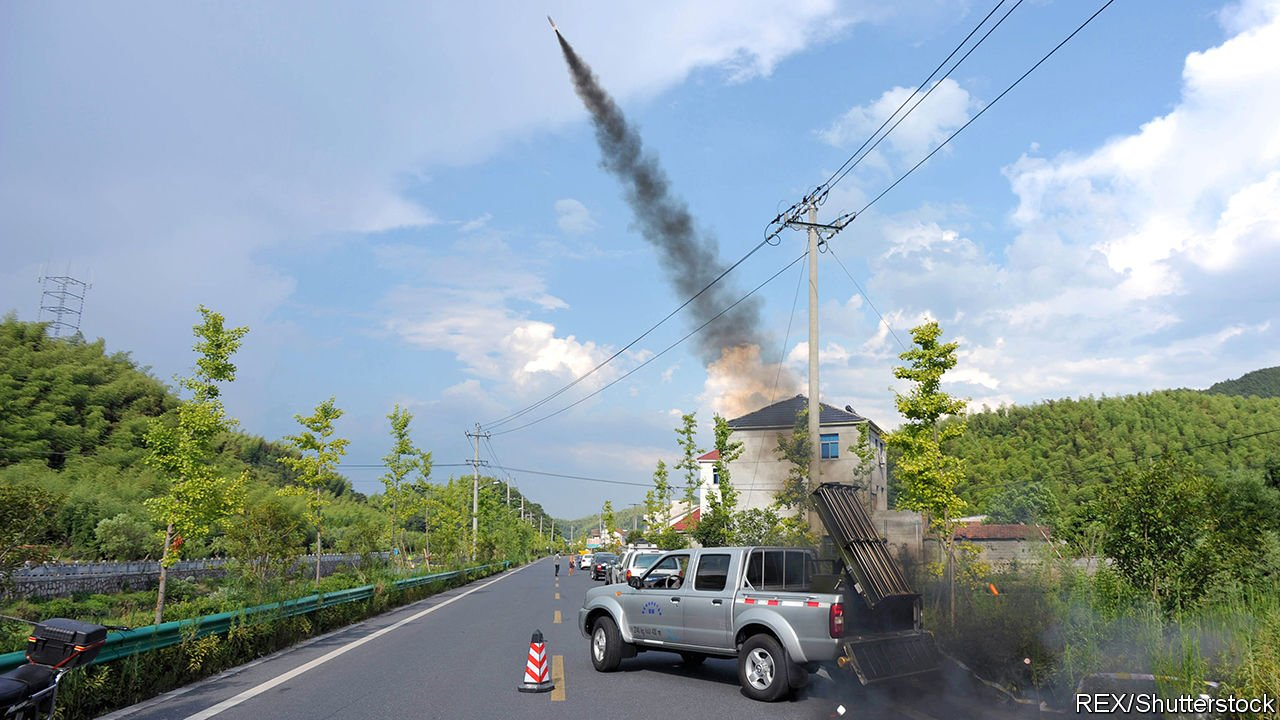
\includegraphics[width=0.8\textwidth]{images/20210327_CNP002_0.jpg}
\end{figure*}
\lettrine{I}N EARLY MARCH a small aeroplane being used by a local weather bureau crashed in a village in the southern province of Jiangxi. All five people on board were killed and one person on the ground was injured. Footage captured on mobile phones showed thick black smoke billowing from the ruins of a house struck by the aircraft, which had been deployed to seed clouds in the hope of causing more rain. 

Such attempts to modify the weather can be dangerous. They require pilots to head into the kind of clouds they would normally avoid. But officials claim that China's efforts to trigger or boost precipitation by scattering chemicals in the sky, which began in the 1950s, have been hugely successful. Today the country spends at least \$200m a year on the programme. In 2018 about 50,000 people were involved in it, most of them part-time or seasonal staff working from small offices in rural areas. Cloud-seeding operations in China cover 5m square kilometres, or more than half of its land territory, according to the government. In December China said it planned to expand this area by around 100,000 square kilometres each year. 

Among the 50 or so countries where cloud-seeding is practised, China is the most enthusiastic promoter of it. The government says the main purpose is to ensure that crops and cities get enough water. In some places cloud-seeding is also intended to prevent hailstorms. Officials claim it can help to put out wildfires and reduce air pollution. State media report that cloud-seeding brings down about 50bn cubic metres of extra rain or snow across the country each year---equal to about 8\% of total water demand. Officials in Beijing claim that in the parched capital, seeding can boost rainfall by 15\%. 

Yet there are more clouds around its effectiveness than China admits. Rainmakers struggle to prove that they can cause any more water to fall than would have been the case otherwise. In 2019 scientists affiliated with the World Meteorological Organisation noted that rainmaking activities were often based on ``empty promises rather than sound science''. 

Recent advances in radar and computer modelling have made rigorous tests more possible. Scientists now generally agree that cloud-seeding can slightly augment snowfall from specific types of cloud that form on the slopes of mountains. Some of China's weather-modification projects take place in such environments. But elsewhere, despite the lack of convincing proof that it works, farmers still want the government to try. And the government likes getting credit when rain does fall. Cloud-seeding creates employment in poor rural places, in particular for army veterans who believe that the government owes them a job. 

Yet the costs are not only financial, as the crash in Jiangxi showed. Only a few of China's rainmakers use planes. More commonly, they fire silver iodide into the sky from artillery pieces. But that can be dangerous, too. Locals are often advised to keep an eye out for unexploded shells, which occasionally land on people's homes. Talking up cloud-seeding distracts attention from better ways of tackling China's water shortages, such as preventing the misuse and pollution of rivers and lakes. It is hard to persuade people to be careful with water while also claiming one can wring it from the skies. {} 
\clearpage
\subsubsection{Chaguan }
\subsection{Chinese divorce courts are places of peril for women }
\paragraph{Print Edition | China  \quad \color{gray}{Mar 27th 2021 }}
\begin{figure*}[h]
\centering

\includegraphics[width=0.8\textwidth]{images/20210327_CND000_0.jpg}
\end{figure*}
\lettrine{A}CCORDING TO THE letter of the law, a Chinese family court should be a safe haven for Wang Fumei (not her real name), a 36-year-old battered wife and mother of two. In-store security cameras were rolling when her husband, a heavy-drinking gambler, came to the shop where she worked in southern China, and beat her without pity. The tape is now with the police. It gives Ms Wang grounds to invoke a law against domestic violence that took effect in 2016, allowing judges to punish abusive partners. 

If called as witnesses, the couple's children would have little reason to defend their father. The 16-year-old son is a migrant labourer---his father refused to pay for vocational training that might have helped the boy into better work. The ten-year-old daughter is scared to hear her father's name. Though safe in her mother's home village, she cannot start middle school this September unless her father hands over the family's household-registration book, or \emph{hukou}, which is needed to enroll her. Even a screenshot would do, the school principal says. Alas, Ms Wang's mother-in-law has told her grand-daughter by telephone: ``Your schooling is not our business.'' On paper, there are other reasons to trust in the law. Ms Wang's meagre income should qualify her for legal aid from the state. The country's supreme court has repeatedly told judges to pay more heed to equality for women. 

In the real world, China's family courts are places of peril for women like Ms Wang. The details are laid out in two books by Chinese-born legal scholars. Between them they draw on thousands of hours of interviews with small-town judges, lawyers and ordinary folk seeking a divorce, many of them rural women whose views of marriage were transformed by their move to a big city. The first work, ``Divorce in China: Institutional Constraints and Gendered Outcomes'' by He Xin of Hong Kong University, was published in January. The second, ``Marriage Unbound: Divorce Litigation, Power and Inequality in Contemporary China'', is by Li Ke of John Jay College of Criminal Justice at the City University of New York. It is due for publication in 2022. 

These studies show how sexism seeps into the work of Chinese divorce courts like a poison in the soil or a miasma in the air. The trouble starts before a judge has even opened a case file. Chinese judges earn promotions by handling cases quickly and for avoiding complaints and appeals. (A typical judge in a family court may hear 200 cases a year.) They are rewarded for pressing plaintiffs to withdraw divorce suits and try once more to patch up their marriages. That is one way to respond to Chinese leaders' angst about soaring divorce rates. In 2019 4.15m couples parted ways. Just 9.47m got married, a record low in modern times. 

Judges routinely refuse first requests for divorce, obliging plaintiffs to come back after a cooling-off period of up to three months. The policy should exclude cases involving violence, but many judges are too scared to declare a husband an abuser. Some judges fear being assaulted themselves. Others worry about presiding over a case that leads to a family murder. Women reporting abuse pose no threat, so they are brushed aside. But men who threaten violence are sometimes bought off with property or even child custody, especially when a son is involved, judges tell Mr He. 

A woman who moves to her husband's rural family home is especially vulnerable, Ms Li finds. Typically she would need to seek divorce in her husband's local court. Often his relatives and neighbours, as well as police officers, decline to testify against a person they see as one of their own. Partly as a result, restraining orders against violent husbands remain vanishingly rare. 

Judges are quick to spot those who arrive in court desperate for a divorce or for custody of a child. They press such needy parties to give up property or make crippling cash payments to a spouse to ``buy'' their freedom. That dynamic hurts women, who initiate 70\% of divorces. In other cases the parent with less money, usually the mother, is simply deemed too poor to keep a child. Judges do not want to spend time haggling over a child-support order, not least because in China such rulings are hard to enforce. 

Ms Wang is vulnerable in all those ways. Desperate to keep her daughter, she needs a court to help obtain their precious \emph{hukou} papers. Worse, even if she were to secure legal aid, state stipends for lawyers are so low that many legal-aid counsel just ``go through the motions'', says a family lawyer in Beijing. 

Stories of suffering abound. Ms Guo, a migrant worker from rural Hebei province, in northern China, watched a female colleague who endured a three-year divorce in court, only to lose both children and have to pay 70,000 yuan (\$10,730) to her husband. In contrast, Ms Guo sought an uncontested divorce from a civil-affairs office. A clerk ended her marriage in 20 minutes because she sought no assets or compensation from her husband, who had found another woman. ``I had a smooth divorce, at great economic and psychological cost,'' she says over Coca-Colas near her factory in Shenzhen. In a Chinese divorce ``all women lose'', she adds. 

That may seem paradoxical. Enough well-meaning laws have been passed to suggest that leaders do want a more female-friendly China. The solution to the puzzle lies in the Communist Party's priorities. Officials sometimes name three goals for the Chinese legal system: delivering justice and fairness, boosting the efficiency of courts and ensuring social stability. But party bosses take a utilitarian, greatest-good-for-the-greatest-number view of human happiness. Thus judges who bully individuals and place efficiency above fairness are just doing their duty. As for maintaining social stability, that is an overriding obsession of party officials. And a reliable way to avoid social unrest is to side with the powerful against the weak. In a Chinese divorce court that means denying women their rights. In an autocratic regime, cruelty is not an accident, it is structural. {} 
\clearpage
\section{Middle East \& Africa }
\subsubsection{Paragon or prison? }
\subsection{The furious debate about Rwanda and its autocratic president }
\paragraph{Print Edition | Middle East \& Africa  \quad \color{gray}{Mar 27th 2021 }}
\begin{figure*}[h]
\centering
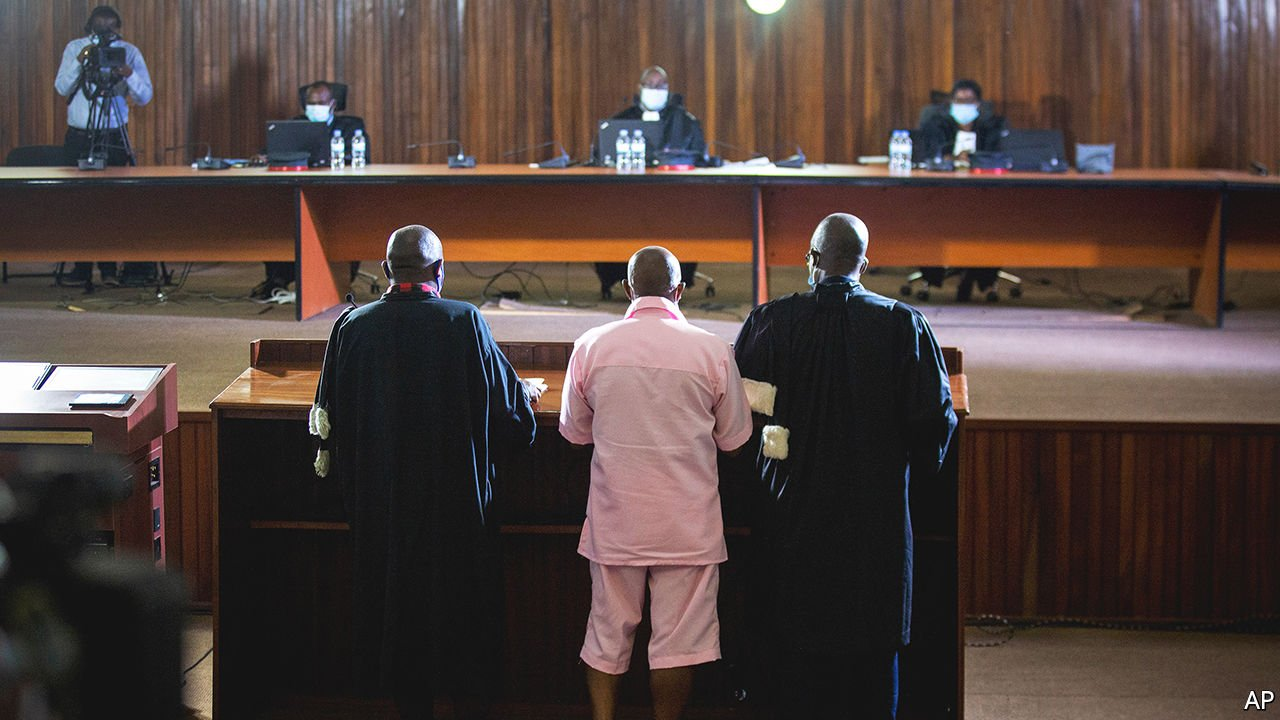
\includegraphics[width=0.8\textwidth]{images/20210327_MAP001_0.jpg}
\end{figure*}
\lettrine{R}WANDA IS PREPARING to put on a show. The Commonwealth Heads of Government Meeting begins on June 21st in Kigali, the capital. And if, despite the pandemic, foreign bigwigs come, President Paul Kagame wants them to be safe, comfortable and impressed. 

Many will be. The streets are clean and quiet. Covid-19 masks are ubiquitous. Citizens form orderly queues to wash their hands outside shops. Some in quarantine are given electronic bracelets to track them. Tony Blair's institute gushes about Rwanda's early vaccine roll-out. 

Some visitors may wonder, though, whether the discipline Mr Kagame imposes on this small, poor African nation goes too far. Police patrol the streets in trucks, rounding up curfew-breakers, who are often forced to spend a night in a stadium without food or water, listening to anti-covid slogans droned relentlessly over speakers. ``I left my house to buy phone credit,'' says Pierre, a middle-aged Kigali resident. ``The police arrested me. It was two minutes before curfew and I explained that I lived in a house nearby. It was very cold in the stadium. There were no blankets.'' 

The streets have also been cleared of beggars, prostitutes and hawkers. Some of those arrested for ``deviant behaviour'' are taught to cook or sew. Others, according to Human Rights Watch, an NGO, are beaten with clubs. ``The conditions were horrendous,'' says Jean, a 16-year-old, who was detained for being homeless. ``We slept on old mattresses teeming with lice. I have scars from the scabies.'' 

A furious debate rages about Rwanda and the man who runs it. Some say Mr Kagame is a hero: that he raised Rwanda from the ashes of genocide and turned it into the most orderly nation in Africa. Others say he is a tyrant whose brutality outweighs any development gains Rwanda has seen on his watch---and that those gains are in any case greatly exaggerated. 

In the first camp are the Rwandan government itself, more or less everyone inside Rwanda who speaks openly, and a chorus of foreign admirers. In the second camp are human-rights groups and Rwandan exiles, including several former members of the regime. The debate is skewed by the fact that Rwandan dissidents live in constant fear of being murdered---even if they are far from home. 

In February Seif Bamporiki, an organiser in South Africa for the Rwanda National Congress (RNC), an opposition group, was shot dead after being lured to a backstreet. It could have been a botched robbery. Violent crime is common in South Africa. But the gun had a silencer, which is unusual. 

``He was one of my best friends,'' says Serge Ndayizeye, who runs a pro-RNC radio station from America. ``His death is not surprising,'' he adds. ``When you kill a leader, people will be afraid to join {[}the opposition{]}. We are fighting an evil man.'' 

Insiders who fall out with the regime are especially vulnerable. Seth Sendashonga, a former interior minister, was shot in Kenya in 1998. Patrick Karegeya, a former intelligence chief, was strangled in a hotel in South Africa in 2013. The government denies involvement in these attacks. But Mr Kagame appears to celebrate them. ``You can't betray Rwanda and not get punished for it,'' he said after the murder of Karegeya, a former schoolfriend of his. 

Mr Ndayizeye was attacked in Amsterdam in 2015, when he was reporting on a ``Rwanda day'' ceremony---when Mr Kagame meets the Rwandan diaspora. Assailants who spoke \emph{kinyarwanda}, the Rwandan language, beat him up in the street. They took his phone; he tracked it flying back to Rwanda. Today he endures a barrage of threats on WhatsApp and Facebook. ``Oh my goodness, it's routine,'' he says. They say things like: ``You will die\ldots{}like Patrick Karegeya.'' 

\href{/node/21799666}{Mr Kagame}'s reputation has taken a battering of late. A new book by a former journalist for the \emph{Financial Times}, Michela Wrong, presents devastating evidence of his cruelty. A recent report by Freedom House, an American NGO, called Rwanda a global leader in intimidating its diaspora. It said the resources it devotes to this are ``stunning'': phones are tapped, social media monitored and expatriates told that their relatives back home will be harmed if they speak out. Rwanda's ambassador to Britain dismisses those conclusions, and says it makes no sense to accuse the government of disregard for human rights when it has progressed so far towards gender equality and environmental sustainability. 

The regime has also attracted unwelcome publicity by kidnapping someone famous: Paul Rusesabagina, who was portrayed in the film ``Hotel Rwanda''. Mr Rusesabagina (pictured on the previous page) saved hundreds of Tutsi lives during the genocide. He initially supported Mr Kagame, but now calls him a tyrant and once appealed for armed struggle to overthrow him. Rwanda calls him a terrorist. The government tricked him into boarding a jet to Kigali, where he was arrested. He will not get a fair trial: a video aired by Al Jazeera showed that the regime has intercepted his communications with his lawyers. ``Kidnapping my father was a message to anyone who dares to speak up against {[}Mr Kagame{]}, that they can get to them, too,'' says his daughter, Carine Kanimba. 

Untangling the truth about Mr Kagame's extraordinary career is not easy. Neither his regime nor his critics always tell the truth. But some facts are uncontested. He was born in 1957. His family fled an anti-Tutsi pogrom when he was a small child, and settled in neighbouring Uganda. As a teenager, he joined a tiny rebel group---a few dozen men with 27 guns---which ended up overthrowing Uganda's dictatorship in 1986. It was the first of at least three governments in three countries that Mr Kagame has had a hand in toppling. 

His old rebel boss, Yoweri Museveni, became (and remains) president of Uganda. Mr Kagame served him as a director of military intelligence. There were many Tutsi exiles in the new Ugandan army, which paid and trained them. In 1990 most suddenly defected and invaded Rwanda to overthrow the Hutu dictatorship. Their leader was killed in the first week. Mr Kagame took over his forces, known as the Rwandan Patriotic Front (RPF). 

The odds were stacked against him. The RPF said it was a movement for all Rwandans, but many Hutus, who were roughly 85\% of the population, saw it as an invading Tutsi army. Still, Mr Kagame managed to seize control of part of the country. A ceasefire in 1993 left neither side satisfied. In April 1994 a plane carrying the Hutu president was shot down. (Who fired the missile is hotly disputed.) Hutu extremists, who had been stockpiling machetes, began a genocide of Tutsis. 

In 100 days the army, Hutu militias and farmers slaughtered perhaps 500,000 people: mostly Tutsis, but also some Hutus who refused to take part. Mr Kagame stopped the genocide by shooting his way to power. He has run the country ever since. 

Stopping the genocide was a great achievement. But some witnesses add details at odds with the monochromatically heroic tale taught in Rwanda today. Ms Wrong spent years interviewing members of the RPF who have fallen out with their leader. They describe a man both brilliant and astonishingly ruthless. 

As a guerrilla in Uganda, he was a master of counter-intelligence, carrying a stick, not a gun. To get rid of a troublesome local government chief, he had a letter drafted thanking him for his help, signed by rebels. The man was executed by his own side. Mr Kagame was also in charge of weeding out traitors. If two rebels who were chatting fell silent when a third appeared, this could be taken as evidence that they were plotting, an ex-rebel told Ms Wrong, requesting anonymity. Some were executed with a single blow to the head with a short-handled hoe, which could also be used to scratch a shallow grave. 

During and shortly after the civil war, RPF fighters massacred tens of thousands of Hutus in Rwanda, according to a suppressed UN report. After Mr Kagame seized power, some 2m Hutus, including many guilty of genocide, fled into Congo (then called Zaire). Some launched raids back into Rwanda. Mr Kagame invaded Congo to crush them, and slaughtered tens of thousands more. 

Congo's dictator, Mobutu Sese Seko, sheltered the \emph{génocidaires}. So Mr Kagame's men marched 1,000 miles across a country 89 times Rwanda's size and overthrew him. In his place they installed a corrupt Congolese guerrilla, Laurent Kabila, and when he refused to take orders from Kigali, they invaded again. The resulting war sucked in several neighbouring states and cost somewhere between 800,000 and 5m lives, mostly from war-induced disease and hunger. It degenerated into a scramble for Congo's minerals, which continues today. Mr Kabila was shot dead by a bodyguard, who was then swiftly killed. No one is sure who ordered the assassination. But Karegeya, Mr Kagame's late spy chief, told Filip Reyntjens of the University of Antwerp that it was Rwanda. 

Mr Kagame's apologists tend to focus on the order he has imposed on Rwanda, rather than the mayhem he uncorked in Congo. Some argue that his ruthlessness is necessary. Were he ever to relax his grip, they fear, Hutu extremists might once again try to eliminate Rwanda's Tutsis. 

\begin{figure*}[h]
\centering
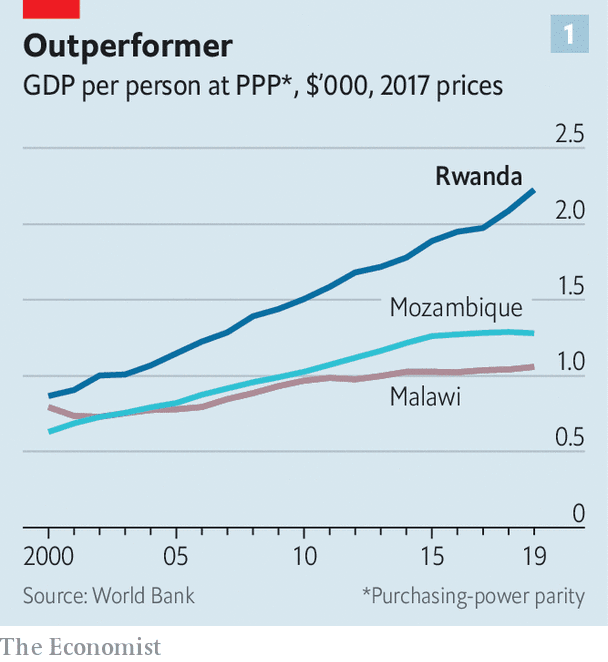
\includegraphics[width=0.4\textwidth]{images/20210327_MAC287.png}
\end{figure*}


His economic record has also persuaded many donors to overlook human-rights abuses. Rwanda has received about 50\% more aid per head than other similarly poor countries in the region such as Mozambique or Malawi (see chart 1). Donors view it as less corrupt and better at using aid to kick-start growth than messier democracies. At first glance, the data bear this out (see chart 2). In the 15 years to 2019, before the pandemic struck, Rwanda posted annual average growth in GDP of almost 8\%. This was double the African average. Granted, Rwanda started from a very low base---the economy shrank by more than 50\% immediately after the genocide. But the IMF thinks it has still grown much faster than might have been expected. 

\begin{figure*}[h]
\centering
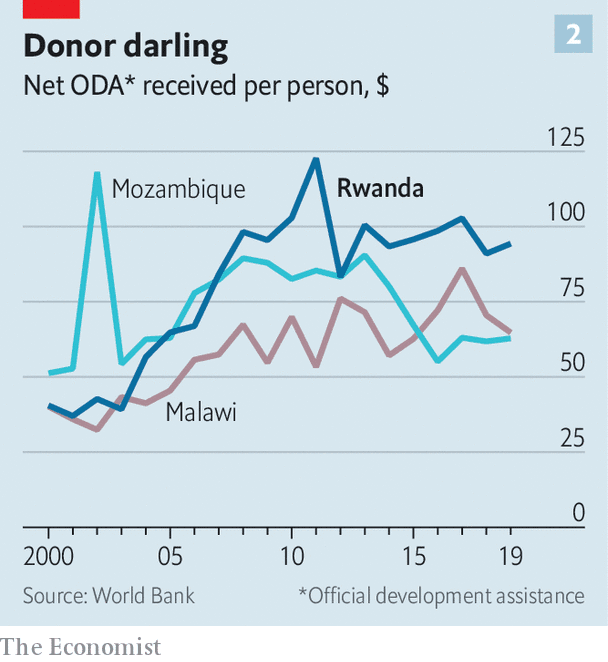
\includegraphics[width=0.4\textwidth]{images/20210327_MAC282.png}
\end{figure*}


``Rwanda's track record, while not perfect, can be seen as one of the best---if not the best---examples where international aid has been effective,'' argues the IMF. Whereas in some countries donors' cash has slipped into politicians' pockets, in Rwanda much of it has been channelled into infrastructure. The results of this can be seen on Kigali's skyline: dozens of shiny new hotels, a brightly coloured conference centre and an efficient airport. 

Mr Kagame's civil service is effective and reasonably meritocratic. Jobs are advertised and applicants sit fair exams (though many Hutus still feel that the plums go to Tutsis). Since 2014 Rwanda has come first in sub-Saharan Africa on the World Bank's annual ranking of the quality of countries' policies and institutions. 

According to official statistics, the pay-off for Rwandans has been large. The poverty rate fell by seven percentage points between 2011 and 2017. Since 2000 the shares of mothers dying in childbirth, and of infants dying, have gone from the worst in east Africa to the best. 

There are worries, however, that some numbers have been manipulated. After the global financial crisis of 2008, Mr Kagame insisted that Rwanda should report improbable GDP growth of 11\%, recalls David Himbara, a former economic adviser. Mr Himbara quit soon after, and now lives in exile and in fear. The IMF quietly estimated that Rwanda's growth that year was 1.7\%. 

Some academics note a discrepancy between consumption per person in the national accounts (which are used to calculate GDP) and calculations based on surveys. In theory both numbers should move in tandem, since they are different ways of measuring roughly the same thing. But since 2005 Rwanda's figures have diverged, with surveys showing that consumption has stagnated, despite seemingly impressive GDP growth. Some economists reckon that the gap between the two had widened to about 50\% by 2013. The government says its figures are sound. 

Rwanda's reduction in poverty has also been questioned. The government employs a lower poverty threshold than most other countries. Using the international threshold of the equivalent of \$1.90 per day, 56\% of Rwandans were extremely poor in 2017, says the World Bank; by the government's measure, 38\% were. Mr Reyntjens reckons that much of the official reduction of poverty is due to a change in the way it was calculated. In 2011 Rwanda's poverty line was based on the cost of buying a basket of food that accurately reflected what poor Rwandans ate. In 2014 it reduced the poverty threshold by 19\% by selecting a different basket, with the same number of calories, that they might in theory buy. Had it not changed the basket, its calculations would have shown that poverty actually rose over that period, rather than falling. 

Not all outsiders agree. Phil Clark of the School of Oriental and African Studies in London thinks that the economists arguing poverty has increased are ``categorically wrong''. ``Anyone who's really looking at Rwanda over the last ten to 15 to 20 years, particularly going out into the countryside, is just struck by how better-off people are than they were at the end of the 1990s or in the early 2000s,'' he says. 

Whatever happened in the years up to 2014, there is now a consensus that progress has, if not ground to a halt, at least slowed. The World Bank reckons that between 2014 and 2017 the share of Rwandans who are poor was stagnant. This was partly because of government policies that discourage people from moving to cities and taking informal jobs, where they would earn more than by staying on the farm, even if they did make the streets noisier. 

The outlook for economic growth is also grim. The pandemic has crushed tourism. Aid, which was worth 17\% of GDP in the fiscal year ending 2006, had fallen to less than 10\% last year. Public debt as a share of GDP has been shooting up---from 26\% in 2013 to a projected 70\% next year. Despite improvements in rankings such as the World Bank's ease of doing business index, Rwanda has struggled to attract much investment. This is partly because its economy is too small to excite multinationals, but also because the ruling party has a habit of muscling in and demanding shares in successful firms started by Rwandans. 

Mr Kagame's intolerance of dissent surely affects the quality of advice he receives. Aides are jumpy. Mr Himbara says he saw Mr Kagame (pictured below) flog his finance director with a cane over a trivial problem involving curtains. Karegeya recounted a conversation from 2003, when Mr Kagame was running for election against a moderate Hutu who has since fled to Belgium. Karegeya suggested that Mr Kagame should claim to have won 65\% of the vote---a solid win, but not ridiculous. The army chief said, no, he should claim 100\%. The official tally gave him 95\%. Karegeya was later jailed for insubordination; he defected soon after he was released. 

How popular is Mr Kagame? It is impossible to say. One ruling-party agent watches each cluster of ten households. ``They know who came to visit you at night. They know what you ate,'' says Mr Ndayizeye, the opposition radio host. In public, Rwandans repeat the official line that there are no Hutus and Tutsis any more, only Rwandans. But do they believe it? 

Odette fled Rwanda in 1994 when she was 11. She has lived in a tarpaulin shack in a refugee camp in Congo ever since. She tried to return home in 2017, but found that her family's farm was occupied by a politician. ``When I told him I wanted the fields back\ldots{}he threatened to kill me,'' she says. ``I was scared to go to the Ministry of Justice, as the Rwandan authorities always end up calling you a \emph{génocidaire}.'' 

For all the rosy development statistics, Rwandans seem miserable. A global happiness survey in 2020 placed Rwanda 150th out of 153 countries, ahead only of Zimbabwe, South Sudan and Afghanistan. 

Mr Kagame constantly shuffles his security team to make it harder for anyone to mount a coup. Opposition groups are scattered and disunited, ranging in ideology from peaceful liberals to violent bigots. Armed groups mount occasional terrorist attacks, but a UN expert reckons there are only a few hundred former \emph{génocidaires} left in the main anti-Rwandan guerrilla groups in Congo. ``Obviously no armed group can walk on Kigali,'' he says. 

Under the current law, Mr Kagame could rule until 2034, when he will be 76. He could presumably change the constitution again to extend his time in office still further. He has offered no succession plan. 

Nic Cheeseman of the University of Birmingham draws a worrying analogy with Ethiopia. Like Rwanda, it was run for many years by a clever, disciplined autocrat who kept a lid on ethnic antagonism and promoted economic development. However, after that strongman, Meles Zenawi, died in 2012, his successors could not hold the country together. Civil war has erupted, along ethnic lines. 

``The main question facing authoritarian development in Africa has always been whether the economic gains achieved under repressive rule are sustainable,'' Mr Cheeseman recently wrote. ``Critics of this model worried that sooner or later, exclusionary political systems would face major challenges from marginalised groups and individuals, and that these challenges could undermine development plans. Recent events in Ethiopia suggest that these fears were well-founded.'' {} 
\clearpage
\subsubsection{Desperate to leave }
\subsection{Saudi Arabia is struggling to end its war in Yemen }
\paragraph{Print Edition | Middle East \& Africa  \quad \color{gray}{Mar 27th 2021 }}
\begin{figure*}[h]
\centering
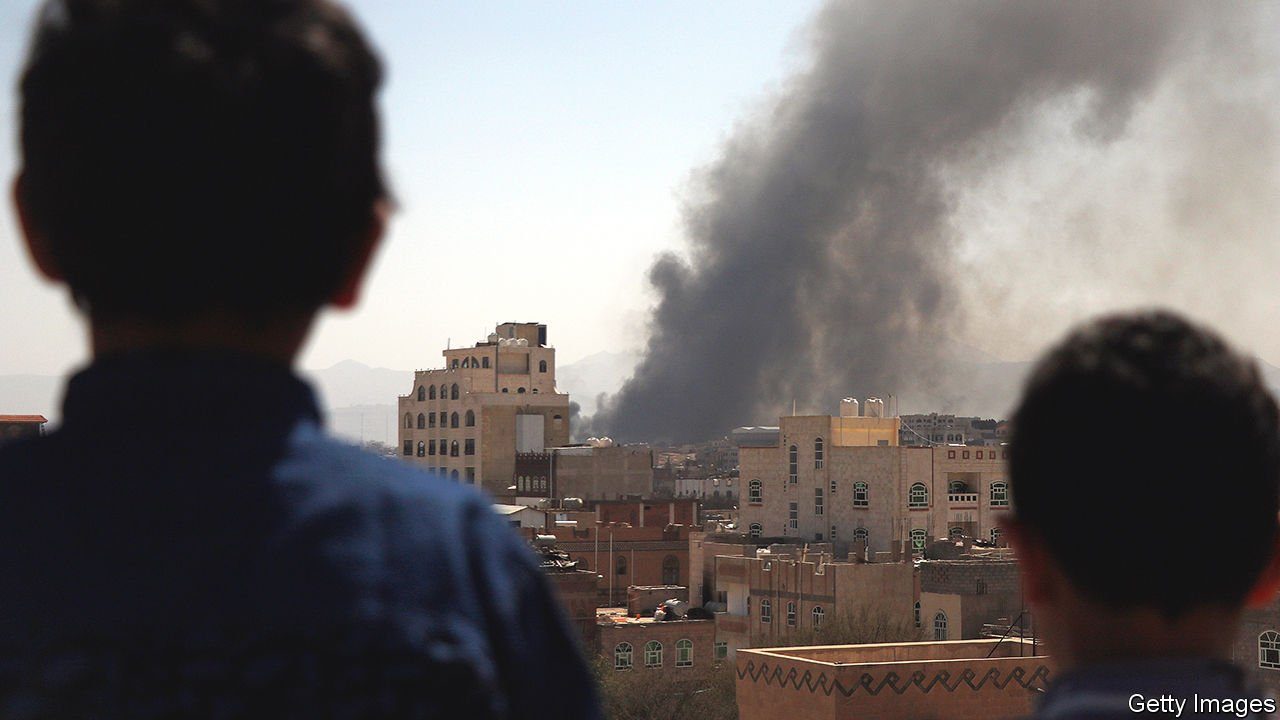
\includegraphics[width=0.8\textwidth]{images/20210327_MAP003_0.jpg}
\end{figure*}
\lettrine{S}IX YEARS have passed since Saudi Arabia declared victory in what it dubbed Operation Decisive Storm, the opening salvo of its war in Yemen. Yet the kingdom is still trying to find its way out of the squall. On March 22nd it offered a ceasefire to its opponent, the Houthis, a Shia militant group that seized control of the Yemeni government (and much of the country) in 2015. The Saudi proposal called for a nationwide truce and offered to ease the air and sea blockade it has imposed on Houthi-controlled territory. ``We want the guns to fall totally silent,'' said Prince Faisal bin Farhan, the foreign minister. 

The Houthis barely paused to consider the offer. Muhammad Abdulsalam, the chief Houthi negotiator, said the Saudi proposal contained nothing ``serious or new''. He was half right: it was serious, but also a warmed-up version of a plan that had failed to win agreement during a year of negotiations. In case the verbal rejection was unclear, the Houthis then sent a drone across the border to attack the airport in Abha in southern Saudi Arabia. The kingdom remains stuck with an intractable dilemma: how do you convince your enemies to end a war they are winning? 

That question has become more urgent as the conflict has grown more catastrophic. More than 112,000 Yemenis have died since the Houthis seized Sana'a, the capital. Millions have been displaced. The Yemeni economy is in ruins, with 80\% of the population reliant on aid to survive. Instead of dislodging the Houthis, the war has pushed them closer to Iran, which gleefully sends military support to bleed its Saudi rival. For this strategic failure, the Saudis have spent tens of billions of dollars, endured a spree of drone and missile attacks, and damaged their standing with partners in the West. 

\begin{figure*}[h]
\centering
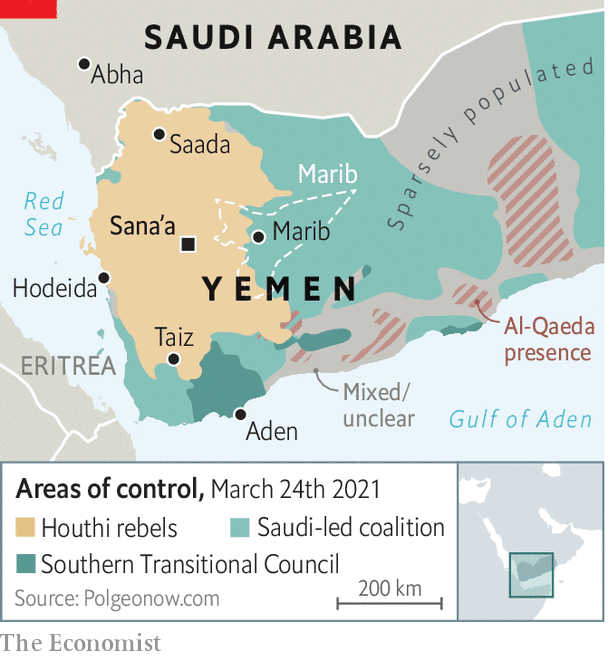
\includegraphics[width=0.4\textwidth]{images/20210327_MAM957.png}
\end{figure*}


Previous attempts at a ceasefire, including a unilateral Saudi truce last year, ended in failure. Both sides say they are open to a deal and have spent the past year in negotiations backed by the UN. But they continue to disagree on the details. The Houthis, for example, want the Saudi-led coalition to lift its blockade of the airport in Sana'a and the port at Hodeida, on the Red Sea. The Saudis are loth to give the Houthis unfettered movement of people and goods---and the revenue that comes with it. They counter by offering limited flights to Sana'a and allowing oil tankers to berth at Hodeida only if taxes and customs revenue are deposited in a special account at the central bank. 

The latest Saudi proposal does not deal with these disagreements---but the act of offering it was itself a negotiating ploy. By doing so in public, the Saudis forced the Houthis to reject it in public. It was an effort to squeeze the group amid a renewed push for diplomacy. Joe Biden, America's president, recently appointed a special envoy to help negotiate a deal. Antony Blinken, Mr Biden's secretary of state, spoke with Prince Faisal on the day he announced the offer. 

But the Houthis are in no mood for making what they see as concessions. After six years of war against a stronger, wealthier foe, they still control the capital and territory containing most of the population. They are pushing ahead with an offensive to capture Marib, the seat of a province with the same name. It is the largest city controlled by the government of Abd Rabbo Mansour Hadi, who is nominally the president of Yemen but governs from exile in Saudi Arabia. Marib is also home to the country's largest oil and gas reserves, and occupies a strategic position along a road that connects to the eastern hinterlands and the Saudi border. Throughout the war it has been a relative oasis of stability, drawing more than 2m people displaced by fighting elsewhere. 

The city has been under indiscriminate rocket and mortar fire for more than a year. In February the Houthis launched one of their periodic ground offensives to capture it. So far the coalition has held them off, and the Houthis have taken heavy casualties. They do not seem to mind the losses, though, as they frequently restock their forces with new conscripts, some of them still children. ``Whenever the Houthis talk about peace with the international community, they escalate their attacks,'' says Sultan al-Arada, the governor of Marib. 

War is its own form of negotiation. The push for Marib gives the Houthis leverage; if they can be convinced to abandon it, they will expect something in return. Both sides will continue to talk, even as they fight. But those talks will be precarious. The Houthis have escalated their missile and drone attacks since the start of the year. Few of these cause serious damage, but a mass-casualty attack could swing Saudi public opinion against a ceasefire. The fall of Marib might embolden the Houthis to push for still more territory. And millions of Yemenis will remain caught in the middle, struggling merely to survive.{} 
\clearpage
\subsubsection{Trouble with the neighbours }
\subsection{Iraqis are getting fed up with Iran }
\paragraph{Print Edition | Middle East \& Africa  \quad \color{gray}{Mar 27th 2021 }}
\begin{figure*}[h]
\centering
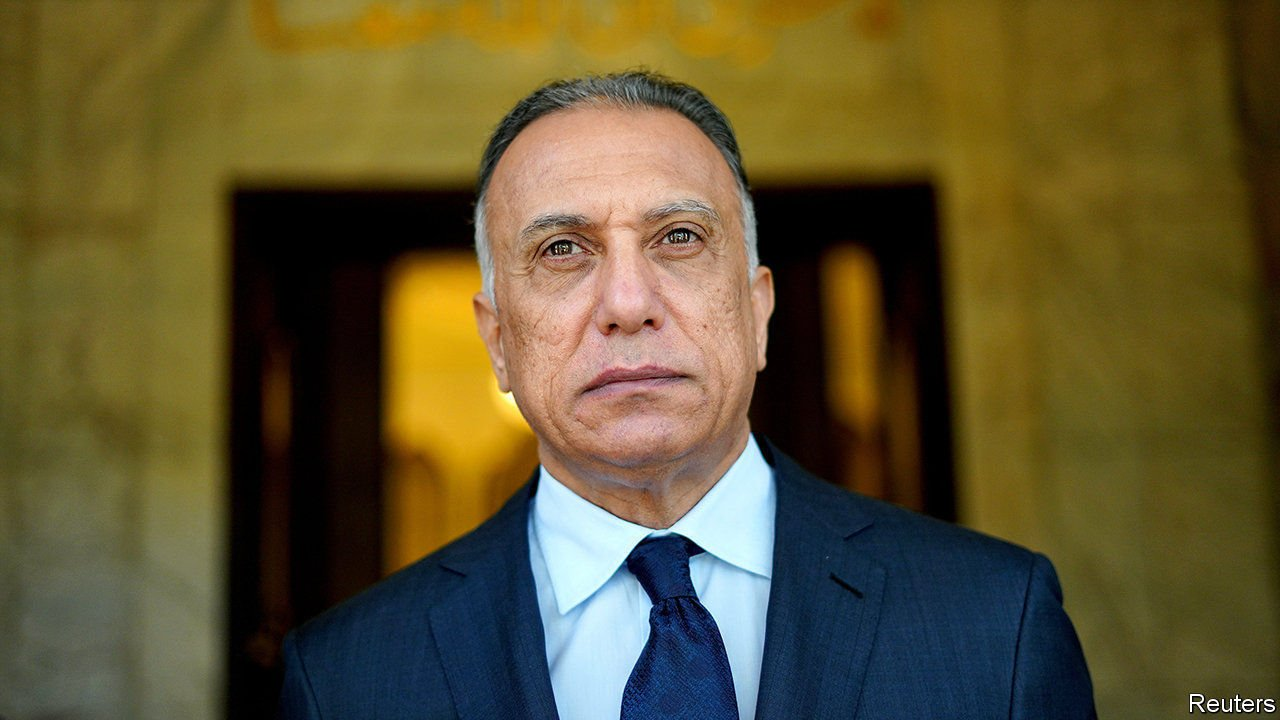
\includegraphics[width=0.8\textwidth]{images/20210327_map505.jpg}
\end{figure*}
\lettrine{``A} STAIN ON Iraq's sovereignty.'' That is how an Iraqi army officer describes the billboard glorifying Qassem Suleimani, a stunningly successful Iranian commander who was killed in an American air strike on Iraqi soil in January 2020. The hoarding looms over Baghdad's administrative district, known as the Green Zone. Many Iraqis once hailed Suleimani as hero for mobilising local forces that beat back the jihadists of Islamic State. But public sentiment in Iraq has turned. The masses who cheered Iran as a liberator increasingly see it as an occupying power. Iraqi politicians are trying to loosen its grip. 

Iranian-backed militias still hold sway in much of Iraq. Many were involved in the violent suppression of anti-government protests that erupted in 2019. Lately, though, they have lowered their profile. They hang fewer placards celebrating their ayatollahs and generals, and appear less often in the streets. They miss the guidance of Suleimani and Abu Mahdi Muhandis, the Iraqi head of an umbrella group of pro-Iranian militias, who was killed in the same air strike. With no clear chain of command, the militias are splintering. They were expected to mark the anniversary of the air strike with a show of force. Thousands of Iraqis marched in Baghdad; the wreck of the car in which Suleimani was killed was displayed. But there were no big retaliatory strikes on American targets. 

Iran has long used Shia politicians in Iraq to assert influence. (Shias are a big majority in Iran and a smaller one in Iraq.) But Iraq's Shia prime minister, Mustafa al-Kadhimi, is not playing ball. Unlike most of his predecessors, Mr Kadhimi is not from a party that is close to Iran. Since taking office in May he has enforced American sanctions, preventing Iran from repatriating the billions of dollars it earns from exports to Iraq. (Ali Shamkhani, the head of Iran's national-security council, summons Iraqi officials to Tehran, Iran's capital, and curses them for not transferring the cash.) The prime minister has also annoyed the militias by restoring state control at some border crossings and removing their men from security posts. At his behest NATO is sending 3,500 new troops. ``These {[}Iranian-backed{]} groups are feeling extremely threatened,'' says Maria Fantappie of the Centre for Humanitarian Dialogue, a conflict-resolution group based in Geneva. 

Such is the level of distrust that foes of Mr Kadhimi, a former intelligence chief, accuse him of passing Suleimani's location to the Americans, enabling the air strike. Militiamen have assassinated Mr Kadhimi's confidants and chased some of his advisers abroad. A group called Kataib Hizbullah, with links to Iran, surrounded his residence in June with pickup trucks full of armed men after he moved to arrest some of its members suspected of killing protesters. ``He was lucky to escape without his head on a plate,'' says an observer in Baghdad. Since then Mr Kadhimi has shied away from confronting the militias directly. His cabinet includes ministers from pro-Iranian factions, who are trying to increase the number of militiamen (already in the tens of thousands) on the government payroll. An Iraqi official recalls the prime minister fretting: ``If you don't pay them, they'll bomb the Americans.'' 

Sometimes they do anyway. Twice this year Iranian-backed militias have fired rockets at American and allied personnel in Iraq. They have also targeted Saudi Arabia: in January explosive-laden drones launched from inside Iraq crashed into a palace in Riyadh, the kingdom's capital. Iraqi officials say militias are massing near the border with Saudi Arabia, armed with 1,400 missiles. Were Mr Kadhimi to become more aggressive, that might also invite a stronger response from Iran, which supplies electricity and gas to Baghdad and other big Iraqi cities. If it cut supply during the summer, unrest would undoubtedly follow. The Iraqi officer peeved by billboards has even bigger worries. If Mr Kadhimi tore down the pictures of Suleimani, he says, Iran might use its proxies to grab Iraq's (mainly Shia) southern provinces. 

Mr Kadhimi's advisers believe that most Iraqis support his efforts to curtail Iran's influence. But in recent elections, they say, the disillusioned masses stayed at home while voters supporting pro-Iranian parties turned out. Another election is scheduled for October. If Mr Kadhimi's men were to do a better job of rallying voters---and if the UN sent monitors to try to ensure a fair poll (a move it is considering)---the political landscape might change in a way that would make his job easier. In the meantime, he has called for a national dialogue that might even include groups under American sanctions. Talking, he seems to have concluded, is better than picking fights he may lose.{} 
\clearpage
\subsubsection{See you again in August }
\subsection{Israel's election has not broken the deadlock }
\paragraph{Print Edition | Middle East \& Africa  \quad \color{gray}{Mar 25th 2021 }}
\begin{figure*}[h]
\centering

\includegraphics[width=0.8\textwidth]{images/20210327_MAP002_0.jpg}
\end{figure*}
As \textbf{The Economist} went to press, there was no clear winner of Israel's parliamentary election, held on March 23rd. The parties expected to support a government led by Binyamin Netanyahu, the current prime minister, are unlikely to win a majority of seats in the Knesset (Israel's 120-seat parliament). But none of his rivals seems to have the support of a majority either. Political stalemate is nothing new for Israel. It has held four elections in less than two years, each failing to produce a stable government. A new election, which would be held this summer, is a distinct possibility. For the latest analysis of the Israeli election, go to Economist.com. 
\clearpage
\section{Europe }
\subsubsection{Erdogan's own goal }
\subsection{A debacle at Turkey's central bank }
\paragraph{Print Edition | Europe  \quad \color{gray}{Mar 25th 2021 }}
\begin{figure*}[h]
\centering
\includegraphics[width=0.8\textwidth]{images/20210327_eup002.jpg}
\end{figure*}
\lettrine{A} WEEK AGO Turkey seemed poised to become this year's emerging-market success story. Foreign investors were pouring back, lured by high interest rates. The central bank sounded serious about taming inflation. The lira was outperforming most of its peers. The economy could look forward to a year of strong growth. 

Then Recep Tayyip Erdogan stepped in. The Turkish president's shocking decision to sack Naci Agbal, the central-bank governor, in the small hours of March 20th set off an earthquake. The lira plunged by 15\% against the dollar as soon as markets opened, before regaining some of its losses. The yield on ten-year lira bonds rose by nearly five percentage points in a day, a new record. The main stockmarket sank by 10\%, reversing all the gains it had made so far this year. Investors, who had bought some \$19bn in Turkish assets since Mr Agbal's appointment last November, began fleeing in droves. During his four months in office, Mr Agbal helped to rebuild the central bank's reputation. Mr Erdogan demolished it with a stroke of his pen. 

Mr Erdogan has now fired three central-bank governors in under two years. Mr Agbal's departure is the most dramatic to date. With a series of overdue interest-rate rises, including a two-percentage-point increase on March 18th, the governor had offered investors a \href{/europe/2021/03/20/naci-agbal-tries-to-restore-monetary-discipline-in-turkey}{glimmer of hope} that the central bank was something other than an extension of Mr Erdogan's government. That hope is now gone. The lira, which had surged back to life after losing half of its dollar value in under four years, is once again on the ropes. Foreign investors feel betrayed. ``These are the worst moments any emerging market has experienced in a quarter of a century,'' wrote Charles Robertson of Renaissance Capital. 

 

Mr Agbal had already been under some pressure. Rumours had been swirling that one of his rivals, Berat Albayrak, who resigned as finance minister a day after Mr Agbal's appointment, might be returning to government. Mr Erdogan, an opponent of high interest rates, must also have been uneasy with the governor's most recent rate rises. But few people expected him to remove Mr Agbal so unceremoniously and so quickly. ``Even if another orthodox candidate will be put in, who knows how long they will stay in charge?'' says Robin Brooks, chief economist at the Institute of International Finance. ``This was basically the final straw.'' 

The new head of the bank, Sahap Kavcioglu, a former ruling-party parliamentarian who is thought to be close to Mr Albayrak, is a relative unknown. Between 2005 and 2015 he was deputy manager at Halkbank, a Turkish state lender which is currently under indictment in America on money-laundering charges. He has sought to contain the damage from his own appointment, saying he would continue efforts to tackle inflation, which reached 15.6\% last month. Investors are unimpressed. Only last month, the new governor echoed Mr Erdogan's view that the key to fighting inflation was lowering rates, a theory widely ridiculed by economists. 

\begin{figure*}[h]
\centering
\includegraphics[width=0.4\textwidth]{images/20210327_euc265_0.png}
\end{figure*}


The brutal market reaction may give Mr Erdogan pause for thought. ``My guess is that it's going to get through to Erdogan that a country with so much foreign debt does not have the freedom to set interest rates as low as it likes,'' says Paul McNamara, investment director at GAM, an asset-management firm. Turkey's president and the central bank may grudgingly surrender to the markets, he says. ``There needs to be a realisation they've bitten off more than they can chew.'' Turkey's short-term foreign debt reached \$140bn in January, around a fifth of GDP. 

That realisation may take time to sink in. Turkey's government may again decide to use stopgap measures, getting state banks to prop up the lira by selling billions of dollars and preventing foreigners from shorting the currency, to pave the way for a rate cut. There are signs this is already happening. Interest rates on overnight swaps for the lira touched 1,400\% on March 23rd, making it hard for investors to dump Turkish assets. But this will be a losing battle, says Phoenix Kalen of Société Générale. Having wasted \$130bn in precious foreign reserves to stem the lira's slide since 2019, the bank lacks firepower. Net reserves have dwindled to \$10.9bn. They are closer to a negative \$40bn when currency swaps with local banks are excluded. 

Mr Erdogan now faces an unenviable choice; to keep rates high and defend the currency, or cut them to boost the economy and risk a currency crash. A more distant risk is capital controls. Turkey's finance minister ruled those out on March 22nd, though some analysts have not. In a country that relies heavily on capital inflows, such controls would bring the economy to a halt. That makes them unlikely, but no longer unthinkable. 

The tragedy is that all this is happening to an economy brimming with potential. Turkey has handled the covid-19 pandemic better than most big European countries. The economy expanded by 1.8\% last year, no mean feat for a country whose tourism sector, which generates upwards of \$30bn in annual revenues, was devastated. Before the central bank earthquake, the IMF predicted that growth would reach 6\% this year. That figure will surely have to be revised downward. Turkey's economy is resilient and dynamic. But as long as it is micromanaged by a strongman whose economic theories give investors the creeps, it will continue to take two steps back for every step forward. Turkey's president was once a semi-professional football player. He may have just scored the worst own goal of his career. {} 

\emph{A version of this article was published online on March 22nd 2021} 
\clearpage
\subsubsection{To have and to hold }
\subsection{Europe's plans to restrict vaccine exports endanger itself---and the world }
\paragraph{Print Edition | Europe  \quad \color{gray}{Mar 25th 2021 }}
\begin{figure*}[h]
\centering
\includegraphics[width=0.8\textwidth]{images/20210327_eud001.jpg}
\end{figure*}
\lettrine{E}VEN BEFORE cases of covid-19 started to surge again, the slow supply of vaccines in Europe was a hot potato. The shortage appears to have an obvious solution. The EU could hold on to more of the covid-19 vaccines that pharmaceutical firms make for export. Thus far EU countries have received 70m doses of vaccines from drugmakers, while exporting 42m doses to 33 countries and getting little or none from abroad. On March 25th, as \emph{The Economist} went to press, European leaders were due to discuss whether greater controls were needed. The proposals suggest halting exports to countries that are not sending jabs back, such as Britain or America, or blocking them to places that have vaccinated more of their population than the EU has. 

Since January, firms wishing to export vaccines from the EU have had to seek permission to do so, a process that involves extra paperwork, missed flights and delays. This move has triggered ripples of concern around the world. Ngozi Okonjo-Iweala, head of the World Trade Organisation, has expressed dismay. These new controls were applied earlier this month, when Italy blocked the export of 250,000 doses of AstraZeneca's vaccine that were destined for Australia. Now the Netherlands says it is ready to prevent the export of the same vaccine to Britain. 

Although the fight with Britain has drawn much of the attention, the EU is also cross with America, which is not letting drug firms export vaccines at all. Furthermore, it has imposed controls on the export of various parts and materials needed to make the vaccines. These controls are already delaying the arrival of crucial items needed in Europe (and elsewhere) to make jabs. Merck, in Germany, must now expand the production of specialist bags that are used to manufacture vaccines and which are running short. America has aggravated matters by not (so far) giving the EU any supplies from a large stockpile of the AstraZeneca vaccine that it has not yet authorised for use. It has, though, sent doses to Canada and Mexico. 

If the EU were to get tough with America over vaccine exports, any retaliation would be likely to have grim consequences for global vaccine production. Little wonder, perhaps, that Germany's chancellor, Angela Merkel, issued a warning on March 23rd that the EU needed to be ``very careful'' with export bans. Even Britain has the power to gum up production of the Pfizer-BioNTech vaccine by withholding an essential raw ingredient, a specialist fat that is needed to make the shot and which is supplied by a firm in Yorkshire. Whether it would take such a drastic step is another matter. 

 

Deploying export controls could damage the EU's reputation. Last year pharmaceutical firms invested in new vaccine-production capacity around the world in order to improve the global supply. A lot of that investment went to Europe. Koen Berden, a trade expert at Vaccines Europe, which represents the industry across the continent, says it was made on the assumption that the bloc was a champion of the open trading system. Firms felt secure knowing that their factories could be used to make vaccines for the whole world. 

Richard Hatchett, head of the Coalition for Epidemic Preparedness Innovations, a group that finances vaccine R\&D, also warns of the dangers of trying to win any vaccine trade war. He says it is hard for political leaders to see every part of a complex supply chain. So the consequences of tit-for-tat exchanges are hard to predict. The knock-on effects of Europe's threats are already being felt. Britain has sent an envoy to India to hunt for additional doses of vaccine from the Serum Institute. But any success will delay the supply of vaccines to the poorest countries that are waiting for supplies from the same source. Both Britain and the EU have given a great deal of financial support to the Covax initiative, which is shipping vaccine from the Serum Institute to poor countries. 

Ursula von der Leyen, the European Commission's head, promised last year to keep the world united against the coronavirus and even helped create a group to promote global collaboration on items such as vaccines. Reality is now biting. But many Europeans look enviously at much higher vaccination rates in America, Britain, Israel and elsewhere, or at the sight of vaccines being exported to countries, such as Australia, that are not facing serious waves of the virus. The temptation to hold on to just a few extra vaccines, if only to fend off political pressure at home, may prove hard to resist. {} 

\textbf{Dig deeper} 

\emph{All our stories relating to the pandemic and the vaccines can be found on our \href{/news/2020/03/11/the-economists-coverage-of-the-coronavirus}{coronavirus hub}. You can also listen to \href{/podcasts/the-jab-a-new-podcast-from-the-economist}{The Jab}, our new podcast on the race between injections and infections, and find trackers showing \href{https://www.economist.com/graphic-detail/tracking-coronavirus-across-the-world}{the global roll-out of vaccines}, \href{https://www.economist.com/graphic-detail/coronavirus-excess-deaths-tracker}{excess deaths by country} and the virus's spread across \href{https://www.economist.com/graphic-detail/tracking-coronavirus-across-europe}{Europe} and \href{https://www.economist.com/graphic-detail/tracking-coronavirus-across-america}{America}.} 

\emph{A version of this article was published online on March 24th 2021} 
\clearpage
\subsubsection{In Circe's lair }
\subsection{A row over land takes Italy back to the Middle Ages }
\paragraph{Print Edition | Europe  \quad \color{gray}{Mar 27th 2021 }}
\begin{figure*}[h]
\centering
\includegraphics[width=0.8\textwidth]{images/20210327_EUP001_0.jpg}
\end{figure*}
\lettrine{T}ROUBLE HAS been brewed on Mount Circeo, south of Rome, ever since it was home to Circe, a legendary sorceress who turned Odysseus's shipmates into pigs. The latest tribulation arrived in envelopes that plopped onto doormats in and around the modern town of San Felice Circeo in recent weeks, and demanded that the occupants stump up five years' back payments of a levy some had no idea they owed. The demands are the latest twist in a dispute with its origins in the Middle Ages. 

Several years ago, says their lawyer, Bianca Maria Menichelli, the heirs of Baron Giovanpaolo James Aguet got together to delegate one of their number to register what they say is their right to ownership of the land in the area. Their claim is based on possession of a fief---a right granted by a feudal overlord in exchange for allegiance or services. In this case, the overlord was a pope. Not even Ms Menichelli knows which one, though she says a document shows the arrangement was already in place by the 13th century. 

After the new kingdom of Italy conquered the popes' domain in the late 19th century, the fief passed to the government of the nascent state. Strapped for cash, the government sold it to a buyer who, in 1898, sold it to Baron Aguet. The fief brought with it not only the ownership of the land, but the right to levy an annual fee on any properties on it. 

Mario Montalbano, a local surveyor, says the baron's descendants stopped collecting the levy at least 60 years ago and most people on Mount Circeo came to believe that they were just like homeowners elsewhere in Italy. But in 2019 those descendants' descendants began to exercise their rights again. Residents who want to sell face having to buy their freeholds, for around 30\% of the value of the property, though Mr Montalbano says it can be much more. And now they are being asked for arrears of the levy, in some cases amounting to as much as €35,000 (\$40,000). A toxic brew that is worthy of Circe herself. 
\clearpage
\subsubsection{The breakwater }
\subsection{Madrid's snap election shakes up Spanish politics }
\paragraph{Print Edition | Europe  \quad \color{gray}{Mar 27th 2021 }}
\begin{figure*}[h]
\centering
\includegraphics[width=0.8\textwidth]{images/20210327_eup502.jpg}
\end{figure*}
\lettrine{A}NTONIO MACHADO, a Spanish poet, once referred to Madrid as ``the breakwater of all the Spains''. That is the effect a snap election for the capital's regional government on May 4th is having on national politics. A polarised campaign has roiled both right and left. The contest has prompted Pablo Iglesias, the leader of Podemos, a hard-left party, to step down as Spain's deputy prime minister to stand in the election himself because, he said, of the risk of ``an extreme right-wing government'' in the capital. For Isabel Díaz Ayuso, the conservative regional president, it is a battle between ``freedom and communism''. In fact the election may be followed by calmer water for Pedro Sánchez, the prime minister, and for Spain itself. 

The election is the indirect consequence of a bungled attempt by Ciudadanos, a declining centrist party, to bring down the conservative regional government in Murcia in which it was the junior partner. Rather than run a similar risk, Ms Ayuso dissolved her own coalition with Ciudadanos and appealed to the voters. 

Home to 6.6m people, the Madrid region is a flagship for the People's Party (PP), led by Pablo Casado, which has governed it since 1995. Its policies of low taxes and light regulation have helped give Madrid one of the fastest economic growth rates in the country. Critics say that the price has been cuts in health care that covid-19 has exposed. Ms Ayuso, a 42-year-old former press officer on the PP's right wing, has been determined to keep Madrid's bars and restaurants open. That may have worsened the pandemic in the capital, but it has also turned her into Mr Sánchez's most visible opponent. Early opinion polls suggest the PP will win around 39\% of the vote, up from 22\% in 2019. Its gains will come largely at the expense of Ciudadanos, which may be in terminal decline. But Ms Ayuso may need the support of Vox, a hard-right party polling around 11\%, to form a government. Its entry into a large regional government for the first time would be a big problem for Mr Casado. 

Mr Iglesias's candidacy is a defensive move. Podemos grew swiftly through alliances, which have unravelled. ``Podemos's main challenge is to strengthen its organisation on the ground to have something to go back to'' when it leaves government, according to Sandra León, a political scientist at Carlos III University in Madrid. Mr Iglesias's past ruthless sidelining of rivals in Podemos makes that harder. His appeal to join forces with a regional party led by Íñigo Errejón, his former deputy, was rebuffed. The left-wing vote will be split between them as well as the Socialists. 

Mr Iglesias is a better campaigner than administrator. His coalition with Mr Sánchez has been an uneasy one. He has called for interventionist policies on the labour market and housing, and aligned with Catalan separatists and Basque former terrorists. After the government managed to approve a budget in December, the prime minister has increasingly ignored his deputy. Yolanda Díaz, the labour minister who will take Mr Iglesias's place in the government, is a less disruptive figure. In choosing to devote himself to leading his party, Mr Iglesias will have more freedom to snipe at the government. But he will almost certainly have less power. Many Spaniards, including Mr Sánchez, will breathe more easily as a result. {} 
\clearpage
\subsubsection{Charlemagne }
\subsection{Why the EU is still wary of America }
\paragraph{Print Edition | Europe  \quad \color{gray}{Mar 27th 2021 }}
\begin{figure*}[h]
\centering
\includegraphics[width=0.8\textwidth]{images/20210327_EUD000_0.jpg}
\end{figure*}
\lettrine{R}OMANTIC GESTURES are difficult in a pandemic. But America and the European Union are trying to rekindle their old passion. Like many people struggling to maintain a long-distance relationship in lockdown, Joe Biden was planning to settle for a video call with EU leaders on March 25th to lay out his vision of their life together. It was intended as a make-up session after what has been a tricky patch. The Biden camp had naively thought not being Donald Trump would make European leaders swoon. Instead, Mr Biden's election in November was swiftly followed by the EU signing an investment agreement with China, a move America saw as neither friendly nor helpful. Things started to improve only a few days ago, after the EU joined forces with America to launch sanctions against Chinese figures involved in persecuting Uyghurs. 

Teaming up to confront China is likely to be more effective than doing so separately. It might also be safer, if China's retaliation is diluted. Indeed, the episode has reminded America and the EU why they work together in the first place. The brief period of history in which America was unchallenged is over. Mr Biden is on the hunt for allies because he needs them. For its part, the EU's geopolitical power depends on its economic size. Its market of 450m rich people is enough to dictate standards for such things as cars and phones; companies sometimes make all their products to Europe's high standards to avoid the cost of having different versions for different regions. But this so-called ``Brussels effect'' will fade as the EU's share of the global economy declines. A strong bond between America and the EU would help both. 

Yet the same problems that strained the transatlantic relationship under Mr Trump remain under Mr Biden. Mr Trump's harrumphing that Europe should spend 2\% of GDP on defence was not a personal whim but a longstanding American demand that its allies must honour their promises. The ``America first'' rhetoric may have gone, but many of its policies are still there, as European grumbling about the country's failure to export vaccines attests. Anyone who these days suggests the revival of a comprehensive free-trade deal between America and the EU is laughed out of the room, with EU leaders now focused on protecting the bloc's market rather than opening it up. 

Besides that, it is difficult for the EU to have a common front with America on Russia when the bloc cannot manage a common policy on the topic with itself. German business will plough on with Nord Stream 2, a pipeline across the Baltic sea from Russia to Germany, ignoring wails from its neighbours and sanctions from America. Smaller differences can still strain the relationship. Though they share a commitment to liberal capitalism, the two sides still find the time to row about everything from subsidies to aeroplanes to tech regulation. America and the EU may both now have the same goals on, say, climate change. But different means of achieving them will end up causing friction. For the EU, a carbon border tax, which would slap levies on imports from polluting countries, is a key part of its plans; for John Kerry, America's climate envoy, the policy is a ``last resort''. 

European politicians are still wary of America, despite the overtures of Mr Biden's White House. The brush with Mr Trump left some leaders arguing that the EU should keep the geopolitical equivalent of a bag packed, ready to flee like a spouse in an unhappy marriage. An unreliable America triggered a hard look at the EU's capabilities and a quest for ``strategic autonomy'', led by Emmanuel Macron, the French president. In this view, European countries have belatedly realised that they have outsourced existential questions to a larger partner that cannot be relied on. For some in Europe, America is the question. For others, though, it is still the answer. French ideas of European autonomy provoke howls in Poland and its Baltic neighbours, for whom America is the only credible bulwark against Russia. But in areas beyond traditional security policy, the search for autonomy is still popular. EU officials wonder aloud about the euro becoming a proper reserve currency, if not replacing the dollar then at least weakening America's ability to use its currency to bully European business. 

Tight ties with America were easier to justify during the cold war, when the Soviet Union scared nearly everyone. Now voters see the relationship as optional, argues Ivan Krastev, a Bulgarian writer, in a paper for the European Council on Foreign Relations (ECFR). Although a chunk of European voters always bridled at American influence on the continent, ultimately Europeans knew there was no other option. Today, a transatlantic gap has emerged. For America, China ranks at the top of the list of security concerns, whereas for the EU it is but one of many. In a survey of 11 European countries by the ECFR, most voters would prefer to stay neutral in any conflict between America and China or Russia. In this way, Europe has taken on the role once enjoyed by Japan during the cold war, argues Mr Krastev: an ally, but ultimately a long way from the main theatre of action. In this view, the EU's quest for more geopolitical clout is not the entry of the EU into great-power politics but an escape from it. 

A happier relationship than under Mr Trump is almost inevitable. But it will still be bumpy with Mr Biden, just as it sometimes was under his predecessors even before Mr Trump. What has changed is that the EU wants to be able to make its own decisions on fundamental topics, an ability that becomes especially cherished now EU leaders know that someone like Mr Trump can end up in the White House. Often the EU's independent aims will be compatible with America's. Their histories are deeply entwined and they have a fundamentally similar world-view. But they will not be identical and they will increasingly diverge, whether on matters small or big. And if two lovers want different things, they often end up drifting apart. {} 

\textbf{\emph{See also:}} \href{https://www.economist.com/tracking-joe-biden}{\emph{We are tracking the Biden administration's progress in its first 100 days}} 
\clearpage
\section{Britain }
\subsubsection{Britain and the European Union }
\subsection{Hopes of a better post-Brexit relationship with the EU are fading }
\paragraph{Print Edition | Britain  \quad \color{gray}{Mar 27th 2021 }}
\begin{figure*}[h]
\centering
\includegraphics[width=0.8\textwidth]{images/20210327_BRD001_0.jpg}
\end{figure*}
\lettrine{S}INCE BECOMING prime minister in July 2019, Boris Johnson has often referred to EU countries as ``our friends and partners''. Many of his fans believed that, once Brexit was done, a more co-operative relationship between the two would be possible. Even those who criticised Mr Johnson's December trade deal for its thinness hoped closer collaboration on issues ranging from the environment to foreign policy would allow Britain and the EU to build on it. Yet three months on, the relationship seems scratchier than ever. 

The year began badly with bigger barriers to trade than many exporters had expected. Covid-19 and stockpiling in the run-up to Brexit make the figures harder to analyse. But in January goods exports to the EU were down by over 40\% from December, whereas they rose marginally to non-EU markets. For fish and shellfish, exports fell by a massive 83\%; for food and drink, by 75\%. Services exports are also likely to have dived. 

Covid-19 vaccine wars now cast another shadow. For much of 2020 the story was of Britain's slower response than the EU`s to the pandemic. This year it has turned into one of British nimbleness in rolling out vaccines, against the EU's woeful sluggishness. Indeed, many Brexiteers trumpet this as proof that they were right to want to leave the bloc. 

The government has been careful not to crow over its success with vaccines, and has shown restraint in the face of the \href{/node/21799718}{EU's vaccine nationalism}. France's Emmanuel Macron cast doubt on the effectiveness of the vaccine produced by AstraZeneca, an Anglo-Swedish firm, and a groundless scare over blood clots, which encouraged vaccine resistance, led many European countries briefly to suspend its use. At the same time, EU leaders complained about AstraZeneca's failure to deliver contracted doses. The European Commission is now taking powers to control vaccine exports, including to Britain; though on March 24th, in an attempt to defuse the row, the two sides issued a joint statement saying they were working together to create a ``win-win situation''. 

Differences over vaccines may be resolved more easily than those over Northern Ireland. Under the Northern Ireland protocol that is included in Britain's withdrawal treaty with the EU, the province remains in effect part of the European single market and customs union. Although Mr Johnson has often denied it, this necessarily entails border and customs controls for goods moving between the province and the rest of the United Kingdom. The resulting obstacles have hindered trade between the two, notably of anything that falls under the regulations covering food, drink and plants, and are threatening the Good Friday Agreement that brought peace to Northern Ireland. 

Unionists, including Northern Ireland's first minister, Arlene Foster, hate the protocol because the border in the Irish Sea widens the gap between these two parts of the United Kingdom. They want it scrapped. But if the protocol went, a hard border would be needed between north and south to protect the single market. Not only would this be near-impossible to police; it would also antagonise republicans, who would dislike the land border as much as unionists dislike the sea border. 

The government remains keen to soften the harshest effects of the protocol. But negotiations in the joint committee supervising it have faltered since Lord Frost, who has replaced Michael Gove as British minister in charge, unilaterally extended grace periods for the application of some controls. The EU has initiated legal action against Britain for this apparent breach of the withdrawal treaty, which follows one first proposed in the internal market bill last September. Lord Frost retorts that the EU itself briefly considered breaching the treaty over vaccine exports in January. With such cavalier behaviour on both sides, trust is in short supply. 

One possible solution to the Northern Ireland conundrum would be for Britain to align formally with the EU's veterinary and food-safety standards, thus minimising checks on food, drink and plants travelling between Great Britain and Northern Ireland while helping British exports to the EU. Simon Hoare, Tory chairman of the Commons Northern Ireland committee, claims it would solve 80\% of the regulatory problems associated with the protocol, but the government is reluctant, partly because of its instinctive aversion to red tape and partly because it thinks that accepting EU food standards would scupper the chances of a free-trade deal with America. Yet if it does not come up with a solution, a US trade deal is scuppered anyway: President Joe Biden and Congress are clear that any breach of the Northern Ireland protocol would kill it. 

Inevitably, in the wake of Brexit, there are other niggles. The European Parliament is deferring its ratification of the December trade deal. Britain is refusing to accord full diplomatic status to the EU's ambassador in London. Still, most Britons want to get on with their big neighbour. A poll this week by Ipsos MORI for the Brussels-based EU-UK forum found 78\% of respondents in favour of close relations. However, only 41\% expect them. The attitudes of both sides do not give much ground for hope. 

The EU's vaccine mess has made it pricklier. That will pass, but one of its main concerns will not: it believes that, if Brexit were seen as a success, it might encourage others to follow suit. That is a reasonable fear; but in Britain, its failure to take into account Northern Ireland's particular characteristics looks insensitive. 

Mr Johnson takes the view that, in the long term, loosening ties with a chronically slow-growing continent and looking instead across the Atlantic and to Asia is the best way of ensuring Britain's future prosperity. In the meantime, keeping a greater distance also makes it easier to blame problems arising from Brexit on European red tape and protectionism. Those wanting a closer relationship across the channel are likely to be disappointed.{} 

\textbf{Dig deeper} 

\emph{All our stories relating to the pandemic and the vaccines can be found on our \href{/news/2020/03/11/the-economists-coverage-of-the-coronavirus}{coronavirus hub}. You can also listen to \href{/podcasts/the-jab-a-new-podcast-from-the-economist}{The Jab}, our new podcast on the race between injections and infections, and find trackers showing \href{https://www.economist.com/graphic-detail/tracking-coronavirus-across-the-world}{the global roll-out of vaccines}, \href{https://www.economist.com/graphic-detail/coronavirus-excess-deaths-tracker}{excess deaths by country} and the virus's spread across \href{https://www.economist.com/graphic-detail/tracking-coronavirus-across-europe}{Europe} and \href{https://www.economist.com/graphic-detail/tracking-coronavirus-across-america}{America}.} \emph{For more coverage of matters relating specifically to Brexit, visit our \href{/brexit}{Brexit hub}.} 
\clearpage
\subsubsection{Asylum }
\subsection{Priti Patel's asylum changes will make life harder for refugees }
\paragraph{Print Edition | Britain  \quad \color{gray}{Mar 27th 2021 }}
\begin{figure*}[h]
\centering
\includegraphics[width=0.8\textwidth]{images/20210327_BRP003_0.jpg}
\end{figure*}
\lettrine{T}HERE IS NO mention of using wave machines or water cannons to blast asylum-seekers crossing the Channel in flimsy boats. Those were reportedly among the ideas mulled by officials to stop the arrival of undocumented migrants. But deterrence remains the object of ``the biggest overhaul of the UK's asylum system in decades'', announced by the home secretary, Priti Patel, on March 24th. Even minus wave machines the proposals are radical. 

At its heart is the idea that the treatment of asylum-seekers will depend on whether they arrived ``legally''. The government will do its best to send back boat people and lorry stowaways to the safe countries through which they travelled. Those who manage to avoid deportation, and persuade the authorities that they are fleeing persecution, will get a right to remain for just 30 months. They will have fewer benefits than claimants who arrive by legal routes and will have ``restricted'' family-unification rights. The Home Office will ``regularly'' assess them for possible deportation. 

The proposal is ``cutting away at the whole principle of asylum'', says Steve Crawshaw of Freedom from Torture, an NGO. Under a widely accepted interpretation of the Refugee Convention, which turns 70 this year, a person's mode of arrival has no bearing on whether he or she is entitled to asylum. People fleeing violence and persecution do not tend to apply for visas and travel by aeroplane: officials are reluctant to issue visas to people they think might claim asylum, and oppressive regimes may stop them from leaving by normal routes. Critics say Ms Patel is creating a two-tier system, which will discriminate against some refugees purely on the basis of their itinerary. 

She contends that she is battling people smugglers, saving migrants' lives and defending women and children who are ``elbowed out of the way by young men'', and that she wants to create ``safe and legal'' ways for refugees to come. She has in mind an expansion of the programme under which since 2015 Britain has plucked 25,000 refugees, mainly Syrians, from refugee camps and resettled them. Such favoured arrivals will immediately be given indefinite leave to remain in Britain---an ``unalloyed good'', says Colin Yeo of Free Movement, an immigration-law website. 

But Ms Patel's focus is on keeping out less worthy claimants and getting rid of those already in the country. In 2019 Britain deported just 7,400 people, the lowest number on record. Ms Patel wants to boost that number. Her ``end-to-end'' reforms of the asylum system will penalise would-be refugees for making claims that the government deems to be in bad faith and set a more rigorous standard for determining whether they face persecution at home. The result, say the refugees' defenders, will be to subject them to more uncertainty than they have already endured. 

Although boatloads of refugees arriving on British beaches make headlines, the country is not being flooded by asylum-seekers. The pandemic has disrupted migration but in 2019, 36,000 people applied for asylum, a third as many as in France. Ms Patel's new rules are unlikely to reduce the number of people seeking refuge in Britain, but they may succeed in treating some of them more shabbily.{} 
\clearpage
\subsubsection{Power rangers }
\subsection{Defence cuts make Britain's armed forces leaner but not meaner }
\paragraph{Print Edition | Britain  \quad \color{gray}{Mar 27th 2021 }}
\begin{figure*}[h]
\centering
\includegraphics[width=0.8\textwidth]{images/20210327_brp501.jpg}
\end{figure*}
\lettrine{A}T AN ARMY base in Dorset, 16 soldiers nestle in the woodland next to dune buggies. Drones, some of them no larger than a sparrow, weave through the conifers above, beaming footage to a phone strapped to each soldier's chest. Specialists in electronic warfare hoover up enemy signals; a member of Britain's 77 Brigade, dedicated to psychological operations, clutches a camera. 

Light, high-tech and globally deployed troops like these lie at the heart of a command paper published by the Ministry of Defence on March 22nd, building on a review of foreign policy the previous week. The soldiers are part of a new £120m (\$165m) ``Ranger Regiment'', modelled on America's Green Berets, which will train and accompany friendly foreign troops and rebels in ``high-threat and hostile environments''. The 1,000-strong regiment will deploy its first battalion next year, probably to east Africa. 

The Rangers are the ``vanguard'' of a new ``expeditionary posture''. Troops will no longer sit in barracks, springing forth in wartime, but will be deployed in hotspots, building influence and countering Russian and Chinese activity. British special forces like the SAS have done this for decades, most recently deploying covertly alongside Kurdish militia to fight Islamic State. The Rangers will do it more frequently, openly and in larger numbers. 

The question is whether such ``permanent and persistent global engagement'' will bend the armed forces out of shape. The paper says the army's mandated strength will shrink by 10,000 to 72,500 troops, its smallest size since 1714. General Sir Nick Carter, chief of the defence staff, insists that it would still be able to produce the same type of force, including the equivalent of an armoured brigade, that it did for the Iraq war 18 years ago. Adding in 30,000 reserves---available on six months' readiness---will bulk out its size beyond 100,000. 

It is true that a smaller force can be a more lethal one. Some of the new British units will have utility in a high-end war. The Royal Marines, for instance, are transforming from traditional amphibious infantry into a roving ``Future Commando Force'', kitted out with kamikaze drones and advanced weapons previously confined to elite special forces. At an exercise in California last year, a company of British commandos defeated a force of 1,500 American marines by infiltrating their rear areas and striking command nodes. 

Army cuts are also offset with new investments. Britain's offensive cyber-capabilities will be offered to NATO. Admiral Tony Radakin, the First Sea Lord, notes that between 2015 and 2030 the Royal Navy's tonnage will grow by 50\%, with seven new classes of submarines and ships---including a new spy ship to monitor undersea cables---all of which will likely be built in Britain. ``That level of shipbuilding in this country hasn't been seen since the 1970s,'' he says. Yet for all that, there is a tangible sense that Britain has long ceased cutting fat, and is now shaving off bone. 

One problem is the loss of ``mass'', in the military jargon. Consider the case of Britain's tanks. The army will upgrade these, but cut the force to just 148---half as many as France. Two regiments of tanks would typically allow an armoured advance along just six kilometres of fighting front, says Jack Watling of the Royal United Services Institute. And if they run into trouble, there is nothing in reserve. 

A lighter, nimbler and more global army also has other weaknesses. Traditionally, combat support---like logistics, engineering and artillery---has been handled centrally by large divisional headquarters, which lend those enablers out to smaller brigades which do the fighting. 

Under the new plans, these enablers will be pushed down into new ``brigade combat teams''. The advantage is that those teams can be deployed more widely, without relying on an unwieldy headquarters above them. The downside is that enablers are spread thinly. ``It is a less efficient system for warfighting,'' says Mr Watling. 

The final problem is one of timing. Many of the cuts create gaps that will not be filled for years. The navy will shrink before swelling to its larger size. The withdrawal of all 700 Warrior infantry fighting vehicles without a comparably armed replacement or suitably long-range artillery leaves infantry dangerously vulnerable as they close with the enemy. 

In many cases, it is not even clear what will fill these gaps. The defence paper is evasive on many details, including the size and timing of investment in drones and autonomous systems, and kicks many decisions down the road.{} 
\clearpage
\subsubsection{Defying gravity }
\subsection{Nicola Sturgeon survives the Alex Salmond affair }
\paragraph{Print Edition | Britain  \quad \color{gray}{Mar 27th 2021 }}
\begin{figure*}[h]
\centering
\includegraphics[width=0.8\textwidth]{images/20210327_brp503.jpg}
\end{figure*}
\lettrine{I}T WAS MARCH 29TH 2018, and in an Edinburgh office building a civil servant's birthday party was under way. After the cake and singing, Geoff Aberdein asked to speak to Nicola Sturgeon, the first minister of Scotland, alone in her office. What happened next is uncertain, for no one else was in the room. 

Mr Aberdein says that during a ten- or 15-minute conversation, he revealed that Alex Salmond---his former boss and Ms Sturgeon's predecessor---was subject to two complaints by former officials. Ms Sturgeon would later tell the Scottish Parliament she was first told of the claims four days later. She insists Mr Aberdein merely urged her to meet Mr Salmond, who was deeply distressed and threatening to resign from the Scottish National Party. ``I had a general sense that it was something serious, something in the realms of a sexual complaint potentially,'' she told James Hamilton, Ireland's former public prosecutor, whom Ms Sturgeon had asked to investigate the claim that she had misled the Scottish Parliament. 

Mr Hamilton's report, published on March 22nd, put an end to a labyrinthine and grubby drama that has consumed Scottish politics for most of the past two years. Mr Salmond stood trial for charges of sexual offences against ten women, and was acquitted. Opposition politicians accused Ms Sturgeon of misleading Parliament by covering up what she knew of his conduct. Mr Salmond accused her inner circle, including her husband, of whipping up complaints in an effort to sink his career and put him in prison. 

Mr Hamilton cleared Ms Sturgeon of four counts of breaching the ministerial code. Her omission of the birthday party meeting led to an ``incomplete narrative of events'', but he accepted her claim that she had forgotten about it. On March 23rd, a second report, by a committee of the Scottish Parliament, split on party lines on the question of whether Ms Sturgeon potentially breached the ministerial code. Later that evening the Scottish Parliament held a confidence vote in Ms Sturgeon; she won by 65 votes to 31. 

The affair has revealed an unflattering picture of Scottish politics, tainted by obfuscation, feuds and a conspiratorial culture. The committee found the Scottish government's processes for handling complaints to be seriously flawed. It recommended the Parliament should be given more powers to scrutinise the executive; a majority of its members concluded they had been left to ``drag'' information out the government. The complainants told the committee that the inquiry had become a partisan circus. 

Still, the two inquiries amounted to more thorough raking-over of alleged misconduct in office than is now customary south of the border. Ms Sturgeon claims that had Mr Hamilton found that she had breached the code, she would have resigned. Whether that is true is unknowable; what is known is that when Priti Patel, the United Kingdom's home secretary, was found to have breached the code by bullying her staff, she refused to resign, and the prime minister declined to sack her. Sir Alex Allan, the government's adviser on the code, resigned in protest. Lord Evans, a former head of MI5 and Mr Johnson's independent adviser on ethics, has asked whether a ``culture of impunity'' is seeping into government. 

On March 25th, campaigning begins for elections to the Scottish Parliament on May 6th. The Conservatives intend to tell voters an unaccountable SNP needs reining in, which will be less fruitful now. Mr Hamilton's findings lend support to her portrayal of herself as a woman blamed for the sins of a man, and the confidence vote as an attempt to bully her out of office. The elections will be, as the SNP wants, mostly about independence. If the SNP returns to government, it will push ahead with legislation for a second referendum, and set the course for an ugly stalemate with the British government which intends to block it. 

For a while, gravity appeared to be returning to Scottish politics. The SNP has been in power since 2007; Ms Sturgeon became deputy first minister while Tony Blair was still in Downing Street. Its record on running education and health is patchy. The Salmond affair painted a picture of a party soiled by too many years in office. Polls before Mr Hamilton's report suggested that trust in the SNP had been dented among around a fifth of the party's supporters. Mr Hamilton's findings may halt the decline, and unleash another blast of hot gas into the balloon. {} 
\clearpage
\subsubsection{Madame Ecosse }
\subsection{Why Scottish women are coming round to independence }
\paragraph{Print Edition | Britain  \quad \color{gray}{Mar 27th 2021 }}
\begin{figure*}[h]
\centering
\includegraphics[width=0.8\textwidth]{images/20210327_brp502.jpg}
\end{figure*}
\lettrine{W}ITH THE possible exception of William Wallace, the best-known Scottish nationalist was, for a while, a woman. In 1967, Winifred Ewing (below), ``a slight, blonde woman in a purple coat'' in the words of one newspaper, became only the second Scottish National Party (SNP) candidate to be elected to Westminster. (The first, Robert McIntyre, only lasted three months.) When she arrived at Parliament, policemen escorted her through a crowd of supporters waving saltires. She soon became known as ``Madame Ecosse''. 

By the time Scotland got its say on independence, in the referendum of 2014, the cause had become a rather more male affair. Nicola Sturgeon, whom Mrs Ewing mentored, played second fiddle to Alex Salmond, then the first minister and party leader. The campaign was, in the words of a female nationalist, ``dominated by shouty men''. And male supporters of independence outnumbered female ones. A narrow majority of men (51\%) and only 42\% of women voted for independence, according to YouGov. ``The women's vote effectively lost the referendum,'' says Elaine C. Smith, a comedian and nationalist campaigner. 

Since the referendum, the gender gap has narrowed sharply. Most polls now either report a negligible gap or suggest independence is more popular among women than men (see chart). If that trend persists, it removes a significant obstacle in the path to independence. What, then, has changed women's minds? 

\begin{figure*}[h]
\centering
\includegraphics[width=0.4\textwidth]{images/20210327_BRC103.png}
\end{figure*}


The most obvious explanation is change at the top. Mr Salmond resigned the day after the referendum. His successor, Ms Sturgeon, is popular with a majority of men but even more so among women. That remains true despite the public mud-slinging between \href{/node/21799714}{Ms Sturgeon and her predecessor}, which culminated this week with an inquiry concluding that she did not break the ministerial code. By contrast, men were much more likely than women to view Mr Salmond favourably. Ms Sturgeon insists on a gender-balanced cabinet (in fact, women outnumber men) and has introduced family-friendly measures like giving a free box of clothes, books and a thermometer to the parents of every new baby. 

Ms Sturgeon's popularity does her cause no harm, but it cannot entirely explain the swing. As Heinz Brandenburg of Strathclyde University points out, the polls started to shift only in 2018, four years after she took the top job. And analysis by the Scottish Centre for Social Research suggests that Mr Salmond was not the only cause of female scepticism last time round, since even women who thought highly of him were less likely to support independence than were men who also rated him highly. 

External factors probably also explain the change. Women tend to be more risk-averse than men. That may account for their lack of enthusiasm for constitutional change in other parts of the UK (see chart). Scottish independence is as risky as ever, but Brexit and the economic uncertainty induced by the pandemic mean that the status quo appears less predictable than it was in 2014, says Ailsa Henderson of Edinburgh University. It may therefore no longer be clear to women which is the least risky option. Ms Henderson has found that women are over-represented among Scots who voted No in the 2014 referendum and against Brexit but now support independence. These days, Mrs Ewing is far from the only Madame Ecosse. {} 
\clearpage
\subsubsection{Very hell }
\subsection{How young Britons are coping with a frozen labour market }
\paragraph{Print Edition | Britain  \quad \color{gray}{Mar 25th 2021 }}
\begin{figure*}[h]
\centering
\includegraphics[width=0.8\textwidth]{images/20210327_brp504.jpg}
\end{figure*}
\lettrine{S}AM HAGGER shut the three pubs he owns in and around Leicester a few days before the government ordered a national lockdown last March. Many of his workers were deeply upset, but the younger ones---about half were under 25---were relatively sanguine. Some even brought cakes and cards to the pubs, as though misfortune had befallen not them but somebody else. 

Had they guessed what was coming, they might have been more anxious. Covid-19 and the measures Britain has deployed to suppress it have disrupted young people's working lives more than anyone else's over the past year. They have responded in ways that are sometimes helpful, sometimes harmful to their prospects. This can be seen in Leicester, a city with a median age of just 32 that has been locked down for an unusually long time. 

Thanks largely to the government's furlough scheme, which pays workers to do nothing, unemployment has not surged. Still, the number of employees in February was 693,000 lower than a year earlier. Of those missing workers, almost two-thirds are under 25; 18- to 24-year-olds are also more likely to be furloughed than any other age group. 

Some of that reflects the ``last in, first out'' hiring-and-firing pattern common in recessions, says Hannah Slaughter of the Resolution Foundation, a think-tank. But the main explanation is that young people cluster in the worst-hit sectors. In 2019, 32\% of 18- to 29-year-old workers were in hospitality, retail or arts and leisure. Young people dominate those industries even more than they did in past decades. 

Young people entering the labour market have an especially hard road. ``The competition has doubled,'' says Sunah, who has been studying finance at De Montfort University. She reckons that companies are concentrating on bringing their many furloughed and remote workers back to the office, and will only begin hiring when they have done that. If she cannot get a graduate job by the summer, she plans to look for part-time retail work. 

Understandably, many are steering clear of the job market altogether. Helped by a mess-up over A-levels, which led to grade inflation last year, 42.6\% of 18-year-olds had applied to university by January 15th, up from 39.5\% a year earlier. Practical courses that seem to lead to jobs (such as medicine) have been especially popular, humanities subjects not so much. 

Those who have jobs cling to them. PPL PRS, a Leicester-based outfit that licenses music, has about 70 staff under the age of 25, many of whom work in its contact centre. In normal times, young call-centre workers hop from job to job, chasing small increases in pay, says Kevin Underdown, head of human resources. These days most are staying put---partly, he says, because they fear that if they leave they could become ineligible for furloughing. 

In normal times young people's pay grows quickly, albeit from low levels. Now that they are moving less, the escalator has slowed down. The Resolution Foundation estimates that the pay of the average 18-to-24-year-old rose by 6\% last year, down from 12.3\% in 2019. Their earnings could be suppressed for years, as happened to people who were in their 20s when the financial crisis hit. 

Mr Hagger's company is beginning to hire again, on the assumption that Britons will flock to pubs when they are allowed to. But he wonders whether young people will be keen to return to work. As he puts it, ``They've had a break in service.'' Many of them have been stuck at home for most of the past year---something that has been miserable, but perhaps also dangerously habit-forming.{} 
\clearpage
\subsubsection{No smoke, no fire }
\subsection{Not even covid-19 has dented firefighters' resistance to change }
\paragraph{Print Edition | Britain  \quad \color{gray}{Mar 27th 2021 }}
\begin{figure*}[h]
\centering
\includegraphics[width=0.8\textwidth]{images/20210327_brp505.jpg}
\end{figure*}
\lettrine{W}HEN THE pandemic hit, firefighters acted as ambulance drivers to relieve pressure on the NHS. But there were limits to their union's willingness to help out: under a deal with local authorities, the Fire Brigades Union (FBU) agreed that its members would deliver food to vulnerable people but not check on their welfare. The deal expired in January, and the union has since urged its members not to volunteer individually to help with the vaccine roll-out. A report from the national inspectorate on March 17th noted that the so-called ``grey book'', which sets the terms and conditions for firefighters, has not been updated since 2009 and leaves ``little room for services to adapt quickly and provide firefighters with necessary flexibility''. 

While working practices have not changed much in two decades, the demands on workers have. Oven chips are one big reason. In the mid-1990s about one in five domestic fires in Britain began with a chip pan, but by the late 2010s that was down to closer to one in 20. Less combustible cooking, fewer smokers and safer electrical appliances have all contributed to a large decline in fires. In two decades, the number of domestic fires has fallen by more than half, while the number of firefighters has declined only slightly. The result is a sharp fall in the ratio of fires to firefighters (see chart). 

The FBU insists that their members are still busy. Car accidents provide another major source of work and false alarms still need to be responded to. But road-accident casualties have also fallen by half in two decades. The total number of incidents to which firefighters were summoned in England has fallen by 40\% over the period. 

\begin{figure*}[h]
\centering
\includegraphics[width=0.4\textwidth]{images/20210327_BRC269.png}
\end{figure*}


Politicians keen on potential cost savings have been eager to reform the service and give it more roles. Cross-training firefighters as paramedics was tried in 2015 but then abandoned. A government review in 2013 argued that £200m (\$275m) of annual savings could be found if Britain's 52 separate fire-and-rescue services were all run at the average level of efficiency or higher. Reforming the service demands considerable political will, and the FBU tends to have more stamina than governments. 

The fire service is perfect territory for union organising. It takes months to train a firefighter. High barriers to entry into the business, high union membership and high public regard combine to give the FBU a lot of industrial clout, which it is not afraid to use. While the fire service was not exempted from the public-sector pay freezes of the past decade, firefighters' earnings, at £31,767 a year, remain well above the national average; and digital technology helps them to work on their own projects during the longueurs between call-outs. ``The hourly rate is pretty good when you think about the time sitting around the station,'' says a firefighter who runs a buy-to-let property business on the side. It is not hard to see why several private firms make a living out of coaching potential firefighters through the process. It's nice work if you can get it. {} 
\clearpage
\subsubsection{Dizzy rascal }
\subsection{What Boris Johnson has in common with Benjamin Disraeli }
\paragraph{Print Edition | Britain  \quad \color{gray}{Mar 27th 2021 }}
\begin{figure*}[h]
\centering
\includegraphics[width=0.8\textwidth]{images/20210327_BRD000_0.jpg}
\end{figure*}
\lettrine{I}N THE 300 years since Robert Walpole invented the office of prime minister, only three of his 54 successors have made their living by their pen: Disraeli, Churchill and Boris Johnson. Mr Johnson models himself on Churchill, but even his most ardent fans recognise the absurdity of the comparison given his hero's unique wartime role. He has far more in common with Disraeli. 

Like Disraeli, Mr Johnson is an outsider, never really trusted by that mysterious but very real entity: ``the establishment''. Disraeli, the grandson of a Jewish-Italian immigrant who sold straw hats, was the only 19th-century prime minister not to attend a public school or Oxbridge. At first glance, Mr Johnson's background looks quite different. He was ``stuffed to the gills with the finest education England could offer'' at Eton and Balliol College, Oxford, as he put it, but he is more exotic than this suggests. The descendant of Turks, who experienced a peripatetic childhood amid chaotic family circumstances, he treats the British ruling class with a combination of contempt and deference similar to Disraeli's. 

Disraeli could never resist the temptation to poke fun at the priggish and pompous, who were hardly in short supply in Victorian England. He mocked his first patron, Peel, for long-windedness (``he traces the steam engine always back to the tea-kettle''), and his great rival, Gladstone, for self-righteousness. Mr Johnson loves taking a pop at neo-Victorians, whether the great and the good spouting platitudes or woke warriors itching to take offence. 

Both men conquered the establishment by turning themselves into brands. Disraeli dressed like a dandy when he was young, favouring a bottle-green jacket, blue trousers and rainbow waistcoat; as prime minister he arranged his hair in a trademark curl on his forehead. Mr Johnson developed his distinctive persona---tousled blond hair, Bertie Wooster manner and rumpled clothes---at school and has been milking it ever since. 

Both were hopeless with money. Disraeli's first big investment was such a disaster that he didn't clear his debts until he was prime minister. His 14 novels were written at speed to keep the wolf from the door, and, at his lowest ebb, the jailers at bay. One of the things that attracted him to Parliament was that MPs couldn't be imprisoned for bankruptcy. And one of the most treasured consequences of political fame was that he could sell a lot more books: during a spell as chancellor he produced a complete edition of his novels, which sold 300,000 copies in a year. 

Mr Johnson's habits of casting off wives (two so far) and siring children (at least six) make it tricky balancing income and spending. He is having such difficulty surviving on his prime-ministerial salary of £162,000 that he and his girlfriend, Carrie Symonds, are contemplating the very Disraelian ploy of setting up a charity, funded by rich donors, to redecorate their Downing Street flat. 

The most damaging charge against the two men is that they risked their country's fortunes (``success is the child of Audacity'' says one of Disraeli's characters) to feed their egos. Disraeli destroyed Peel's reforming government only to adopt his predecessor's policies of free trade and religious toleration as prime minister. Mr Johnson embraced Brexit at least in part because he thought that it would ease his path to the top. But beneath the shape-shifting, two themes run through the politics of both men. 

The first is the nation-state. Disraeli saw European politics as a clash between the rival principles of ``nationalism'' and ``cosmopolitanism'', and argued consistently that the Conservative Party was a ``national party'' or nothing. That meant celebrating the empire with all due pomp and circumstance and solving the problem of the ``two nations'' that he had identified in his novel ``Sybil'', by promoting harmony between the classes. 

Historians, being nit-pickers by trade, have taken to questioning Disraeli's commitment to ``one-nation Toryism'', pointing out that he had a habit of falling asleep when social reforms were mentioned. But this ignores the importance of his second great political theme: imagination. He thought that politics was less about drafting laws than about spinning stories. He seldom gave a speech without mentioning Britain's glorious past or conjuring up its even more splendid future. And he was so successful in envisioning a ``national party'' that his successors dedicated themselves to turning it into a reality. In April 1883 the \emph{Times} credited him with being the first to discern ``the Conservative working man as the sculptor perceives the angel prisoned in a block of marble''. In the same year the Tories created the mass-membership Primrose League, named after his favourite flower, to appeal to the newly expanded electorate with a socialism-slaying combination of hierarchy, empire and social reform. 

Mr Johnson treats the European Union as the perfect cosmopolitan foil: a self-consciously post-national institution that combines grand aspirations with pettifogging bureaucracy. But he also understands that the Tories cannot merely demonise the opposition. They have to demonstrate that the nation-state can solve people's problems, by increasing funding for the health service and persuading those who feel left behind by the smug, prosperous south-east that they are valued members of the community. He follows Disraeli's example in making up for a shortage of detail with a surplus of imagination: his speeches are an amalgam of references to past glories and vague promises to create a space programme or build a bridge from Scotland to Northern Ireland. It may be empty stuff, but it appeals to present-day ``angels in marble''---former Labour voters who are tired of hearing their country demonised as a nursery of genocide and slavery. 

Randolph Churchill, Winston's father and a posthumous follower of Disraeli's, provided a lapidary summary of his hero's career: ``failure, failure, failure, partial success, renewed failure, ultimate and complete triumph''. Mr Johnson's fortunes have been similarly volatile so far. The ultimate verdict on him may be triumph or disaster, but it is unlikely to be in between.{} 
\clearpage
\section{International }
\subsubsection{Banged up }
\subsection{Brain injuries are startlingly common among those who have committed crimes }
\paragraph{Print Edition | International  \quad \color{gray}{Mar 27th 2021 }}
\begin{figure*}[h]
\centering
\includegraphics[width=0.8\textwidth]{images/20210327_IRD001_0.jpg}
\end{figure*}
\lettrine{M}ANUEL SUFFERED two serious brain injuries as a child in Denver, Colorado. The first was the result of a fall. The second occurred when someone threw a rock at his head, causing him to lose consciousness. He made it the short distance home before blacking out. On both occasions he received brain scans but he does not remember getting any other treatment. 

As a teenager, Manuel was sent to a school for disruptive children. In his early 20s he tried to strangle his stepfather who, he says, was violent towards his mother. He was sent to prison. Last year he suffered a third brain injury when he fell out of a pickup truck travelling at high speed. He spent six days in a coma. When he woke up he had no recollection of what had happened. He was later jailed yet again for violating his parole. 

Manuel's story is far from unusual. Brain injuries affect about 8.5\% of the general population but rates among prisoners are far higher. Kim Gorgens, a neuropsychologist at the University of Denver, reckons that between 50\% and 80\% of prisoners and those on parole in America have brain injuries. A review of research in America, Australia and Europe suggests that the average reported rate is around 46\%. Research conducted in 2010 by Huw Williams of the University of Exeter put the rate among men in British prisons at 65\%. A study published in 2017 found that nearly half of all prisoners in New Zealand had been hospitalised for a traumatic brain injury before committing their crime. Researchers suspect that the numbers may be even higher in poorer countries because road-traffic accidents and violence are generally more common. 

People who sustain brain injuries are more likely to go on to commit crimes, including violent ones. They are more troublesome while in prison and more likely to reoffend on release. This is especially true for those, like Manuel, who are injured as children. Adrian Raine, a psychologist and criminologist at the University of Pennsylvania, is pretty convinced that there is a causal link. He points to research that follows people over time, as well as natural experiments in which otherwise law-abiding individuals suffer a brain injury and then display antisocial behaviour. ``It's a bit like saying smoking doesn't cause lung cancer,'' Dr Raine explains. ``Most people do not get lung cancer. We will never do a randomised controlled trial for it. But do we act on it? Sure we do.'' 

For many the damage is done early. Brain injuries are particularly common among boys and young men, whose brains are still maturing. Those from poor backgrounds who live in cities are especially at risk. A curious child who is rarely supervised is more likely to fall and seriously hurt himself. A reckless adolescent who thinks he is invincible is more likely to crash his car or get punched in the head. They are then far more likely to drop out of school and end up in prison. Brain injuries are one of many risk factors for crime which disproportionately fall on poor people (though most lead law-abiding lives). 

People tend to associate traumatic brain injuries with sports such as American football, boxing and rugby. In fact they are more usually caused by falls, road-traffic accidents and fights. The front of the brain, where the frontal and temporal lobes are located, is often damaged. Higher emotions, such as compassion, seem to be concentrated there, as does conscious decision-making. Long-term memory formation is mediated by the hippocampi, which are in the temporal lobes. Broca's area and Wernicke's area, both important in the development of language, are located in the frontal and temporal lobes respectively. 

The longer a person is unconscious, and the more injuries they sustain, the more severe the effects. People become forgetful. Many find it hard to concentrate. They may struggle to manage their emotions and to understand the feelings of others. Their behaviour and personality may change, although many sufferers fail to recognise this in themselves. 

Brain injuries seem to make a minority of people more violent. Paul (not his real name) had a number of minor convictions when he was involved in an accident which caused a bleed on his brain and left him in a coma. After that his crimes became more violent. Since his accident he has done things that were ``out of character'', he says from a prison in Wales. He knows that he has hurt people but he does not remember his crimes. ``When I get told later on what I've done and what's happened, I'm gutted.'' 

Seena Fazel of the University of Oxford has made cross-references between Swedish health-care and crime records. He found that people who had gone to hospital for a brain injury were more than three times more likely then to commit violent crimes than the rest of the population. They were also twice as likely to do so as their siblings. Damage to the prefrontal cortex, which seems to increase aggression and impulsiveness, may explain this. Another Swedish study found that almost half of a sample of (mostly old) patients with frontotemporal dementia exhibited criminal behaviour. The figure for those with Alzheimer's in the same study was 15\%. 

Michael has a scar on his head where he was hit by a car at the age of seven. None of his six siblings has ever been in any serious trouble, but he started stealing cars and motorbikes and breaking into factories when he was a teenager. Drugs made his problems worse. He also suffered from anxiety and depression. Michael is now in his 50s. He reckons that he has spent more than 20 years in prison over the course of his life. 

His experience fits with what Dr Gorgens has found studying inmates and probationers with traumatic brain injuries in Colorado. Some 96\% had problems with substance abuse and 79\% suffered from some kind of mental illness. It is a vicious cycle, says Dr Gorgens. Substance abuse is more likely in people who have suffered brain injuries, and people with brain injuries are more likely to develop addictions. Separate research shows that after suffering a brain injury, people with mental-health problems were four to seven times more likely to commit a crime than before. When you are dealing with so many problems at the same time, it is easy for them to spiral out of control, explains Dr Gorgens. This is especially true for those who have alienated their family and friends, as people with brain injuries tend to do. They are more likely to end up homeless, unemployed and to commit suicide. 

Michael has turned his life around. He and other campaigners want officials to acknowledge the problem of brain injuries among prisoners. Some are beginning to do so. The British and Australian governments are carrying out reviews of how they treat such offenders. They are also looking at a broader set of ``neurodiverse'' conditions which are disproportionally common among inmates, including learning and intellectual disabilities and autism. Criminal-justice systems need to work better for those whose brains work differently. That might also reduce crime. 

In New Zealand, a pioneer in this field, the focus has been on reforming courts. Andrew Becroft, a judge who used to run the Youth Court, was shocked by how many young offenders had neuro-disabilities. ``History will judge us very harshly,'' he says. The court now screens defendants for brain injuries and has tried to adapt its procedures to take account of their needs. So does the Young Adult List court, which deals with 18- to 25-year-olds. Officers of the court talk to defendants in clear English instead of legal jargon, and provide handouts to those who struggle to understand what is being said. ``It's fundamentally a matter of fairness,'' says John Walker, the court's founder and chief judge. ``If a person came into the court who couldn't speak English, they would be given an interpreter.'' He argues the same should be true for those with neuro-disabilities. 

\begin{figure*}[h]
\centering
\includegraphics[width=0.4\textwidth]{images/20210327_IRD002_0.jpg}
\end{figure*}


Philippa Birch works for the Disability Trust, a British charity that trains people to go into prisons to raise awareness of brain injuries among inmates and staff. People working in prisons often think those with brain injuries come across as aggressive or rude, says Ms Birch. They stand too close or do not pay attention to instructions. She explains the effects of brain injury and reassures prisoners about how they can manage them. Prisoners find lessons in controlling their emotions and anger particularly helpful. Overworked prison staff are grateful for the smoother interactions. 

TBI in Criminal Justice, a collaboration between the University of Denver, various charities and the Colorado courts and sheriff departments, is helping prisoners with brain injuries adapt better to prison and prepare for the world beyond. Some learn how to use a diary to get to appointments on time. Others master breathing techniques to help them stay calm under pressure. These cheap but effective strategies can be the difference between someone avoiding a needless parole violation and going straight back to prison. The team hopes the project will reduce the state's recidivism rates which, at 50\%, are among the highest in the country. 

Some could benefit from better medical treatment. That might mean medication: antidepressants for anxiety or stimulants for fatigue and improved cognitive function. But in the long term most treatments for brain injuries are largely therapeutic. Neuro-rehabilitation relies on recognising that the brain is to an extent able to adapt its structure and function, a process known as neuroplasticity. Physical and speech therapy can help people regain lost function. Computerised ``brain training'' games can improve recall and attention. The earlier and more intense the intervention, the better the prospects of recovery. But coping strategies can be taught at any stage after an injury. 

Identifying those who need support could prevent people from drifting into crime. Mr Becroft, now New Zealand's children's commissioner, argues that children should be screened for brain injuries and other neuro-disabilities when they start secondary school to ensure that those who need help get it. Campaigners are also keen to prevent more brain injuries from happening in the first place. That might mean teaching parents about the risks, or encouraging people to wear helmets. 

A report in 2016 by the Centre for Mental Health estimated that in Britain the cost of traumatic brain injury in a 15-year-old who goes on to offend is around £345,000 (\$475,000). The cost to those affected---and society more widely---is incalculable. {} 
\clearpage
\section{Technology Quarterly }
\subsubsection{The year of learning dangerously }
\subsection{Covid-19 has shown what modern biomedicine can do }
\paragraph{Print Edition | Technology Quarterly  \quad \color{gray}{Mar 23rd 2021 }}
\begin{figure*}[h]
\centering
\includegraphics[width=0.8\textwidth]{images/20210327_tqd001.jpg}
\end{figure*}
\lettrine{T}HE NUMBER of deaths officially attributed to covid-19 now stands somewhere over 2.5m. It is a terrible toll, but hardly an unprecedented one. The ongoing HIV/AIDS pandemic has killed between ten and 20 times as many worldwide. The death toll from the influenza pandemic of 1968 is believed to have been similar to that of covid-19, with a range of 1m to 4m, and until the past year you would have been hard put to find a mention of it outside a medical text. Similarly the flu of 1957. Yet covid-19 has had social, economic and political impacts beyond those of any other health crisis in modern history. 

There is no starker illustration of the fact that, in the body politic as in the bodies the virus infects, the host's response can matter far more to the course of the disease than the direct action of the pathogen itself. An infection which many do not even notice causes in some an immune response which can be fatal. Pandemics, too, are shaped by and reveal the particulars of the world they hit. 

The covid-19 pandemic struck in an age more thoroughly interconnected and information-saturated than any which has come before. Though China was shamefully opaque early on, there was no way the situation could be kept from the world for long. In 1957 Britain's Ministry of Health suppressed estimates that that year's flu might infect a fifth of the population; it would be, in the words of a junior minister, ``a heaven-sent opportunity for the press during the `silly season'\,''. Many politicians have lied and prevaricated about covid-19. None has been able to simply keep schtum. 

The policy response, too, has been one only possible in the information age. The closing of workplaces and shops would have been impossibly disruptive just ten years ago. The shortcomings of Zoom, Microsoft Teams, Amazon and all the other services that the well-off world has relied on are manifest. But their benefits have been vital. 

The greatest technological revelation, though, has been the medical and public-health responses. That the internet has changed the world is not news. That basic biomedical science is now in a position to do so is. Labs were running specific tests for a never-before-seen virus barely a month after the first cases were reported. Crucial information on which therapies, old and new, did and did not work was available by the middle of the year. The evolution of the virus was revealed as it happened by genome sequencing on a scale to which no previous pathogen had ever been subjected. Most remarkably of all, a range of safe and effective vaccines based on various novel approaches was available within a year. One of the technologies used---directly injected mRNA---opens up all sorts of further possibilities. 

This Technology Quarterly will examine how the response to covid-19 has revealed the true potential---and, sometimes, the failings---of these various technologies. It is not, yet, a tale of triumph. But the pandemic has laid bare a hard-won corpus of technological achievement just waiting to be harnessed to the cause of a better future.{} 

\textbf{Dig deeper} 

\emph{All our stories relating to the pandemic and the vaccines can be found on our \href{/news/2020/03/11/the-economists-coverage-of-the-coronavirus}{coronavirus hub}. You can also listen to \href{/podcasts/the-jab-a-new-podcast-from-the-economist}{The Jab}, our new podcast on the race between injections and infections, and find trackers showing \href{https://www.economist.com/graphic-detail/tracking-coronavirus-across-the-world}{the global roll-out of vaccines}, \href{https://www.economist.com/graphic-detail/coronavirus-excess-deaths-tracker}{excess deaths by country} and the virus's spread across \href{https://www.economist.com/graphic-detail/tracking-coronavirus-across-europe}{Europe} and \href{https://www.economist.com/graphic-detail/tracking-coronavirus-across-america}{America}.} 
\clearpage
\subsubsection{After a flying start }
\subsection{Testing and tracing could have worked better against covid-19 }
\paragraph{Print Edition | Technology Quarterly  \quad \color{gray}{Mar 23rd 2021 }}
\begin{figure*}[h]
\centering
\includegraphics[width=0.8\textwidth]{images/20210327_tqd002.jpg}
\end{figure*}
\lettrine{T} HE FIRST outbreak of a novel disease is the opening scene of a whodunnit. In 1976, when more than two dozen members of the American Legion died after a convention in Philadelphia, public-health officials spent months scouring the hotel they had met in before finally tracking down the culprit in the water tank on the roof: a new bacterium which, having caused the first known cases of Legionnaires' disease, was named \emph{Legionella}. In the 1980s it took years of hard work and acrimonious argument among epidemiologists and virologists to blame the terrible and varied symptoms of AIDS on HIV, a virus of a type never previously seen in humans. 

For covid-19, the mystery was solved almost as soon as it had begun. The novel pneumonia that doctors in Wuhan noticed in December 2019 immediately brought to mind Severe Acute Respiratory Syndrome (SARS), a disease caused by a coronavirus which broke out in 2002. As a result of SARS and the subsequent outbreak in 2012 of Middle East Respiratory Syndrome (MERS), also caused by a coronavirus, there were already established protocols for growing cells from the lining of the nose, throat and lungs in order to look for coronavirus infection. They were soon put to use. 

To identify the possible coronavirus responsible meant producing a sequence of its genome. The first step in this process was to extract RNA---the molecule on which coronavirus genomes are written---from the cell cultures. The genetic sequences in these RNA molecules then had to be transcribed into complementary bits of DNA, because that is what automated sequencing machines work with (see part A of diagram). 

\begin{figure*}[h]
\centering
\includegraphics[width=0.4\textwidth]{images/20210327_TQC933.png}
\end{figure*}


Computer programs assembled the sequences those machines produced into a recognisable, if gappy, coronavirus genome. Researchers used this to make DNA ``primers'' with which to fish out the not-yet-sequenced bits of the genome. Finished sequences were published less than two weeks after the process had begun. On January 12th 2020 the world knew its enemy---soon thereafter named SARS-CoV-2---down to the last letter of its genome. 

In terms of the science done, this was all routine; the appropriate use of standard laboratory techniques. In terms of its impact, it was enormous. Knowing the viral sequence was fundamental to vaccination efforts, made it possible to track the virus's evolution and, most immediately, made it possible to test people with a cough and see if they were infected. The first AIDS tests were not available until four years after medical science became aware of the condition they tested for. For SARS it took six months. Procedures for testing swabs from the nose and throat for RNA from SARS-CoV-2 were published 11 days after the genome sequence, on January 23rd. 

There was, however, a drawback to the tests. They required suitably equipped laboratories. Most countries did not have nearly enough of the relevant lab capacity; in others, much of it was being used for different things. ``Prior to March 23rd my lab had never performed a viral diagnostic,'' says Stacey Gabriel, who runs genetic-sequencing operations at the Broad Institute in Cambridge, Massachusetts. But with public institutions swamped she and her colleagues created one of the largest testing shops on America's east coast from scratch, reconfiguring the specialised robots that populate one of the world's most advanced cancer-genetics labs to do the grunt work. 

Dr Gabriel learned two lessons in the process. The first is that uniformity matters a lot. The Broad started off testing samples from Massachusetts nursing homes which came in containers of varying size and with various amounts of liquid, some accompanied by handwritten forms, some by barcodes. Dealing with such messiness is no task for a robot, and so to begin with just a few thousand samples a day passed through machines capable of handling far more. The second is that you need software to track the whole process. Commercial software, dry swabs and barcoding soon had the lab firing on all cylinders. By March 2021 it could handle 200,000 tests a day and was serving customers as far afield as New York. 

The data such labs produce are not just for patients and doctors. In most countries covid-19 is a notifiable disease; the authorities have a legal right to know who has been found to be infected. When a sample tests positive the lab has to pass the identity of the person it came from on to public-health officials. At that point a new sort of detective work begins: where did that person---the index case, in public-health speak---pick up the virus? To whom might they have given it? 

Several East Asian countries demonstrated that, if started in the earliest days of an epidemic and pursued with vigour and persistence, such contact tracing can be a powerful tool. Some, such as Singapore and Taiwan, benefited in this from their experience with SARS in the mid-2000s; tracing systems set in place back then were put to use with an urgency born of experience. A level of invasiveness from which most Western authorities shied away was often employed. In South Korea, for instance, contact tracers were able to download a list of all financial transactions made by those who tested positive; they could then obtain CCTV footage from shops the index case had visited in search of other customers to check up on. ``{[}Such snooping{]} has come up with discussions I've had with policymakers,'' says Christophe Fraser, a digital epidemiologist at the University of Oxford. ``We got very hung up on the idea of contact tracing disrupting people's lives.'' 

Western governments acted in a slower, less thoroughgoing way. They failed to track the initial spread, in part because of insufficient testing capacity (and, in America, dud tests from the Centres for Disease Control and Prevention). They ended up with much less impressive systems. Tom Frieden, a former director of the CDC, says he thinks that, at its current level of effort, America could plausibly trace about 15,000 cases a day---a level that has been handsomely exceeded every day since April 2nd 2020. Britain has earmarked £37bn for testing and tracing over the 2020 and 2021 financial years, and though it may well spend less, the shoddiness that has dogged some elements of the campaign, such as a database cock-up which lost thousands of results in September 2020, will be remembered. 

\begin{figure*}[h]
\centering
\includegraphics[width=0.4\textwidth]{images/20210327_tqc144.png}
\end{figure*}


A basic problem is that contact tracing is a lot of work. Theoretical assessments based on analysing social networks and experience in Asia both suggest that some 30 contacts need to be identified for each index case. Digital tools can lessen the load. Resolve to Save Lives, a campaign run by Vital Strategies, an NGO, developed Locator, which taps into credit data to help tracers track down people who may have caught the virus from a specific index case. But the amount of work required remained enormous. 

A much discussed alternative to such programmes was to use the world's most ubiquitous tracking devices: smartphones. Google and Apple worked together to develop a system which enabled phones to keep a list of occasions when they were near another phone for a significant period of time, and the identity of that second phone. When someone tests positive for SARS-CoV-2 they are asked to send a message from their phone which is used to notify all the other phones they had been near within a particular window of time. But everything is peer-to-peer; neither the big tech companies nor the public-health authorities get a list of contacts. 

Unfortunately this built-in privacy makes it hard to assess the technology's efficacy. British and Swiss studies suggest such apps do reduce spread, but not enough to make them more than an also-ran technology. None of the successful contact-tracing systems in East Asia relies on such things to any significant extent. 

Even without good tracing, self isolation of those who tested positive helped slow the spread of the disease. But over time the shortcomings of the initial testing technology, reverse-transcriptase polymerase chain reaction (RT-PCR), became ever more apparent. It is conceptually elegant (see diagram) and easy for labs to use. But despite its familiarity, reliability and sensitivity, it has real disadvantages. 

One is that it needs labs, and is carried out most efficiently in big ones. This means samples may have to travel a long way. It also means that they can get held in queues. The Broad runs its RT-PCR tests in just three and a half hours; but the average sample takes 15 hours to process. Results from RT-PCR tests normally come in days not minutes. 

\begin{figure*}[h]
\centering
\includegraphics[width=0.4\textwidth]{images/20210327_tqc142.png}
\end{figure*}


Another problem is that though the presence of viral RNA clearly shows that a person has been infected, it says very little about where they stand in the course of the disease; RNA is detectible from very soon after infection to long after the disease has run its course. In public-health terms what is needed is a test that spots people who are actually infectious---people with cells in their noses and throats actively churning out virus particles. 

To look for the SARS-CoV-2 particles themselves means looking for their distinctive protein components, not for the RNA that tells cells how to make them. The most detectible such component is the spike protein which studs the particles' outer membranes. And one of the basic rules of modern biotechnology is that when you want to find a protein, use an antibody. 

Antibodies are large molecules that come in millions of varieties, each of which sticks to one target---known as that antibody's ``antigen''---and one target only. A handy technology called lateral-flow testing makes use of that specificity. A sample is placed at one end of a porous membrane and, as it seeps along to the other, encounters a line of antibodies designed to recognise it. When the sample is urine and the antigen is a hormone found in expectant women, you have a pregnancy test. When the sample is mucus from a swab and the antigen is the spike protein, it is a covid-19 test---a cheap, convenient one which can provide results with in half an hour. Such tests may not pick up all the people in whom RT-PCR might detect a trace of the virus. But if their nose and throat cells are not producing enough antigen for the test to detect, they are probably not producing enough to be infectious, either. 

At the beginning of the epidemic ``the supply chain for the lateral-flow tests wasn't there,'' says Dr Gabriel. Chris Hand, the chairman of Abingdon Health, a British contract manufacturer of lateral-flow tests, says the main bottleneck was the speciality membranes that are part of every test kit. ``They come on large reels of 100 metres plus, which go through automated equipment to add biochemicals by spraying them at low volumes,'' he says. But once the biochemicals---the bespoke antibodies and some more generic bits and bobs---are ready, the production processes in place and the packaging sorted, the tests could be churned out by the million. 

New technologies now reaching the market will further change the dynamics of test and trace. QuantuMDx is one of a number of companies developing automated PCR-in-a-box systems that provide results within a couple of hours. Jonathan O'Halloran, the firm's boss, says the British company has been relying on its own testing system for the past 22 weeks, testing its 90 staff members every morning (they are free to decline). About once a week lunchtime brings the news that someone has tested positive; they are immediately sent home to isolate. When things are done this fast, the fact that RNA is detectable before people are infectious is a plus; isolating on the basis of an early PCR test means no one ever turns up to work infectious. The company claims not to have lost a single day to infection. 

A combination of local, automated PCR and lateral-flow tests could be the basis of an ideal testing system---one which has a chance of keeping ahead of, and containing, a low level of disease rather than lagging behind one that is shooting up. Antigen tests would be used to scan the population for new infections. Those found would be referred to contact tracers; contacts who might have been infected could then be PCR-tested to find out which of them actually were. 

Great for public health. No benefit, in itself, to the index cases who would wait, isolated, to see what fate the virus and their immune systems had in store for them---painfully aware that their next encounter with the wonders of modern medical technology could be in a hospital bed. {} 
\clearpage
\subsubsection{Finding what works }
\subsection{Well conceived drug trials have saved hundreds of thousands of lives }
\paragraph{Print Edition | Technology Quarterly  \quad \color{gray}{Mar 23rd 2021 }}
\begin{figure*}[h]
\centering
\includegraphics[width=0.8\textwidth]{images/20210327_tqd003.jpg}
\end{figure*}
\lettrine{I}N FEBRUARY 2020 doctors from the World Health Organisation (WHO), visiting China to see the ward- and morgue-filling reality of covid-19, found more than 200 clinical trials under way. Desperate to help dying patients, doctors in Wuhan and elsewhere had been scouring their dispensaries for plausible treatments. They were trying out antiviral drugs developed to treat other viruses, anti-inflammatory and other drugs that modulate immune responses, antibody-rich blood plasma from people who had recovered, traditional Chinese medicines of various sorts and more. In each case there was at least some reason to hope that the treatment might do some good. But the trials were all too small to see if those hopes were being borne out. 

Drugs are a difficult, and expensive, technology to work with because---unlike, say, a computer chip---they can be useful even if they only work in some cases, and telling those that work some of the time from those that don't work at all requires big clinical trials. Seeing the pandemic heading their way, doctors and health systems in other countries scrambled to set some up. Drug companies, for their part, started to work on the only targeted drugs they know how to develop from scratch in months: antibodies. 

In March 2020 the WHO set up Solidarity, a trial which eventually enrolled 12,000 patients in 30 countries. It looked at the effects of various existing antivirals used to treat HIV and Ebola, as well as an antimalarial drug, hydroxychloroquine, which seemed in laboratory studies to have had an effect on SARS-CoV, the virus behind the SARS outbreak of 2002-03. Six months on, none of the treatments was found to reduce mortality or the need for mechanical ventilation; nor did they shorten hospital stays. 

Though disappointing, this was not surprising. Antivirals have never had the stopping power or the broad range of actions that the best antibiotics used to fight bacteria can boast. This is because killing bacteria, as antibiotics do, is a fundamentally simpler problem than stopping viruses. Bacteria are cells in their own right which depend on lots of distinctive molecular mechanisms to stay alive. An antibiotic that knocks out one of those mechanisms can be effective against many sorts of bacteria while leaving human cells, which lack the relevant mechanism, unscathed. 

Antivirals, by contrast, must either tweak the inner workings of cells to make them inimical to viruses or target one of the handful of viral proteins required for infection or replication. The first option has historically led to a great many side effects. New technologies, though, might allow a more targeted approach that aims at some factor in the host which the virus absolutely requires and the host can do without. The CRISPR gene-editing system makes it possible to create tens of thousands of cell lines each lacking just one gene; finding out which of these cell lines a virus cannot get on with shows which host proteins it most depends on. Applied to SARS-cov-2 this screening technology has turned up various host factors worth looking at, some of which are already drug targets, but there is no human trial data to go on as yet. 

The alternative to going after host factors is targeting a system which the virus provides for itself, such as the one it uses to copy its genome when reproducing. Remdesivir, a drug developed by Gilead, an American pharmaceutical company, does this by mimicking one of the building blocks of RNA. When the virus's genome-copying mechanism uses this molecule instead of the proper building block, it crashes. 

Remdesivir did not pan out as a treatment for hepatitis C, the virus for which it was originally designed, and though it has some effect against Ebola other treatments work better. When Solidarity tried remdesivir against SARS-CoV-2 it found no benefit. But three smaller trials, some with patients in earlier stages of infection when antivirals work best, found it reduced the length of hospital stays (though did not save lives). Fifty countries, including America, have approved it for use, but the WHO remains unconvinced of its merits. 

Though there are still some other antivirals in trials, ``I think we have pushed about as far as one can with repurposing,'' says Francis Collins, the director of America's National Institutes of Health. ``You really need to have something more targeted.'' The Rapidly Emerging Antiviral Drug Development Initiative, or READDI, based at the University of North Carolina, aims to make sure that when the next pandemic virus comes along there are better targeted antivirals to meet it. It is seeking to develop broad-spectrum drugs against the viral families with the most pandemic potential: coronaviruses, flaviviruses (such as Zika and West Nile virus) and alphaviruses (such as chikungunya, a mosquito-borne disease). The goal is to have, by 2025, stockpiles of five promising drugs that have passed safety trials in humans and are ready for application. It is focusing on drugs given orally, which can be used early and widely. Remdesivir's modest results may stem from its need for intravenous administration. It is only used in hospital patients for whom its time has passed. 

If antivirals have underwhelmed, a cheap anti-inflammatory drug has been a life saver. The means of demonstrating this was RECOVERY, a clinical trial which covers all of Britain's hospitals. Martin Landray of Oxford University rushed to get RECOVERY integrated into the clinical-trials system within the National Health Service before wards began to overflow. The effort paid off, allowing recruitment into RECOVERY to become a possibility for most covid-19 patients referred to hospital. It enrolled more than 11,000 patients in 175 hospitals in its first three months, and has published results on six treatments. 

Dexamethasone, the benefits of which RECOVERY had demonstrated by June 2020, is a corticosteroid which acts as an anti-inflammatory. Inflammation is part of the body's natural defence against infections and other challenges. Immune cells sensing something amiss in their neighbourhood send out signals which cause nearby blood vessels to dilate and leak. That causes redness, swelling and pain while allowing more immune cells to gain access to the site. With covid-19, as with a variety of other infections, this response can go too far, compromising infected organs. 

Steroids can stop that. The problem is that if they dampen down the immune response before it has the virus at bay they may do more harm than good, says Ralph Baric of the University of North Carolina. RECOVERY showed that the best time to start dexamethasone is when patients first needed to be given oxygen. 

Quickly adopted as the standard of care all around the world dexamethasone has been credited with saving more than 600,000 lives. Survival rates have also been improved by experience. Early on, patients with low oxygen levels were put on mechanical ventilators too readily. After blood clots were found to be common in severe covid-19 cases, blood-thinners became a routine hospital treatment. In Britain the death rate among hospitalised patients has fallen from 31\% in March-May 2020 to about 12\%. 

This February the RECOVERY trial showed that tocilizumab, another drug which dampens down immune responses, also reduces the risk of death from covid-19, confirming results from an earlier European trial. Tocilizumab, like all drugs with names ending in -mab, is an antibody---a class of drugs for which the market has quadrupled over the past decade. 

The immune system uses antibodies to fight pathogens. When they stick to virus particles they can stop the virus from getting into cells. When they stick to cells infected by a virus they tag them as targets for other bits of the immune system to attack. 

The pharmaceutical industry tends to use the antibodies it makes in cell cultures to different ends: not to target alien molecules, but to target molecules the body is making to its own detriment, most notably in cancers and autoimmune diseases. All the big-selling antibody drugs cater to these markets. Tocilizumab blocks the action of interleukin-6, a messenger molecule which plays a role in inflammation; it was developed to lessen the symptoms of rheumatoid arthritis. Other antibodies which modulate the immune system are still in trials as covid-19 treatments. 

But some antibodies have been developed as treatments for infections. Last year America's FDA approved two antibody drugs for Ebola; there are now a large number of antibodies for SARS-CoV-2 in trials. It has been possible to get them into the pipeline quickly because of the way they are developed. Finding an immune-system cell that produces the antibody you want, tweaking the relevant genes and putting them into cells devoted to antibody production is a lot faster than sifting through vast libraries of chemicals to find those with the most promise, learning how to make them into medicines, proving them not to be toxic and so on. 

A year into the pandemic antibody treatments made by two American drug companies, Regeneron and Eli Lilly, have been approved by regulators. Each is a cocktail of two different antibodies, and each has to be infused through an intravenous drip. But both are approved for use only in patients with mild to moderate illness, or those who are at risk of becoming ill. They are contraindicated for those already sick enough to be admitted to hospital. Even if their potential beneficiaries feel it worth having infusions when not that sick, the practicalities of providing such a service to people who should be isolating at home are daunting. Nearly 1m doses of the two drugs that have been bought and distributed by America's federal government have gone unused. 

What is more, the \href{/node/21799637}{spike protein} at which the antibodies are aimed is evolving. Researchers need antibodies that recognise these new variants, too. George Scangos is the chief executive of Vir Biotechnology, which makes an antibody recently shown in trials to reduce hospitalisation or death by 85\%. He describes how his team selected it because it binds to a bit of the SARS-CoV-2 spike protein that looks the same as its equivalent in SARS-CoV, the virus which causes SARS. The thinking was that, if evolution had kept it the same, it was probably because it could not be changed without weakening the virus. But Dr Scangos says it is possible that viral evolution will, in time, catch up with their cleverness, and that the team will have to find further antibodies to be used in combination with this one. 

The ideal would be a system that can make lots of slightly different antibodies at once, makes them exactly where the patient wants them, and can be programmed in advance to churn them out as required. Happily, almost all human bodies come equipped with just such a production line, in the cells of the immune system. And in the most impressive of all medicine's responses to the covid-19 pandemic, new vaccine technology is now putting those production lines to use in millions of people every day. {} 
\clearpage
\subsubsection{A nucleic-acid revolution }
\subsection{Novel vaccines have performed remarkably quickly and well }
\paragraph{Print Edition | Technology Quarterly  \quad \color{gray}{Mar 23rd 2021 }}
\begin{figure*}[h]
\centering
\includegraphics[width=0.8\textwidth]{images/20210327_tqd004.jpg}
\end{figure*}
\lettrine{O}N NOVEMBER 30TH 1803 the \emph{María Pita}, a 160-tonne corvette, set sail from Spain for the New World. King Charles IV was keen that his subjects over the ocean benefit from the new technology of vaccination, which used inoculation with pus from blisters due to cowpox, a comparatively minor ailment, to engender immunity against smallpox, a scourge which killed millions---including, a decade earlier, the king's beloved daughter. 

The initial challenge faced by the man in charge of this expedition, Francisco Balmis, was how to get viable cowpox across the ocean. His solution was to take on board 22 boys from an orphanage, two of whom he had infected with cowpox beforehand. During the voyage West the infection was kept viable by being carefully spread from boy to boy, and over the four years which followed, the virus transported and nurtured within them was used to inoculate hundreds of thousands of people from Peru to the Philippines. (Balmis relied on a fresh supply of orphans obtained in Mexico to get the virus safely across the Pacific.) 

The Balmis expedition provides a striking illustration of a basic truth. Creating vaccines is a job for biology, and doing biology requires living systems. From Edward Jenner's discovery in 1796 that cowpox could be used as a vaccine---the word vaccination, coined shortly thereafter, is derived from the Latin \emph{vacca}, for cow---all the vaccines humankind has used to protect itself were produced in living cells. Until last year. 

Over the course of the pandemic a fundamentally new vaccine technology has come into its own. When the first, spectacularly positive results from phase 3 trials of the Pfizer/BioNTech mRNA vaccine were released on November 9th they did not just offer a pandemic exit strategy. They also showed, as did the results of the similar vaccine made by Moderna, that the long process through which science has abstracted biological mechanisms from their fleshy and fibrous substrates has reached a new level. In a small but vital way, medicine has begun to look like programming. 

For a long time vaccine production was an often messy and sometimes disgusting business. The polio vaccine developed by Jonas Salk in the 1950s was made in vats of minced kidneys, a process which required thousands of rhesus monkeys to be farmed and killed. In the 1968 flu pandemic Maurice Hilleman, and American virologist, got through chicken eggs by the tonne as he grew 9m vaccine doses in their yolks in just four months. 

Though the chicken-egg method is still used for flu vaccines today, later vaccine-makers worked out how to grow soups of individual vaccine producing cells---cell cultures---in vats large enough to supply what was needed to control all sorts of other diseases. Doing so made things safer as well as easier. The polio vaccines made from viruses grown in minced monkey kidneys also contained a somewhat dodgy looking virus, now known as SV-40, that was not detected until it had been injected into tens of millions of people. Had it been carcinogenic---there is no evidence that it was, though some debate on the matter continues---it would have been a disaster to make a nuclear meltdown look small-bore. 

But the manufacturing systems that are being used to make the vaccines against covid-19 currently being administered at a rate of millions per day are something else again. They do not produce weakened versions of the virus being vaccinated against, like those used in flu jabs and later versions of the polio vaccine. They do not even produce specific antigens. Instead they just send a message: the genetic sequence which describes the SARS-CoV-2 spike protein. When presented as messenger RNA, or mRNA, this message gets cells to produce the protein just as they would if they were infected by the virus. That gives the immune system a risk-free preview of what infection would look like, allowing it to develop its response ahead of time. 

The new vaccines deliver their message in two different ways. In the Oxford/AstraZeneca, Johnson\&Johnson and Sputnik V vaccines it is contained in a protein shell derived from an adenovirus. Cells are engineered to make adenovirus particles which have a DNA version of the sequence that describes the spike protein nestled inside them. The particles they produce are then harvested to make vaccine. The adenovirus gets the DNA into the vaccinee's cells; the cells transcribe the DNA into mRNA which they then use to make spike proteins. 

Harvesting virus from a cell culture is hardly a new form of vaccine-making. But the adenovirus, as used in this system, is not really the vaccine. It is not there to produce an immune response to itself. It is the platform which allows the DNA within to get into cells and set about producing antigen there. 

An important part of this is that the message in the DNA is independent of the particles into which it is packed and of the cultured cells that do the packing. The same manufacturing infrastructure---the same recipe for growth medium, easily modified versions of the cells, identical protocols---could be used to load a different DNA sequence into particles which would look just the same. The system is not an interconnected whole, as biological systems are in nature. It has been rendered modular. 

This modularity is helping vaccine companies produce second-generation jabs that protect against variants of SARS-CoV-2 with which the first generation may cope poorly (see next chapter). Insert the DNA for a version of the spike protein which engenders a better response, reboot the system and off you go. In principle the companies might use the same approach to deliver the DNA for a completely different antigen, and thus a vaccine against a completely different disease. ``It's very different from making vaccines in the old days,'' says Greg Lemke, a biologist at the Salk Institute (yes, same Salk). ``Then every vaccine was a new project with a whole new infrastructure. With these technologies, every new vaccine is the same project.'' 

The second of the new technologies, mRNA, works on similarly modular lines, but is yet more radical. A DNA version of the spike gene is used to make huge amounts of mRNA in a cell-free system---a solution that contains an enzyme called RNA polymerase, the chemicals that power its work, and the raw components from which RNA is made, all of which can be bought off the shelf. The mRNA thus produced is then packaged into tiny particles of lipid---the inert material from which the membranes around cells are made. After the original DNA has been harvested no cells are involved. It is all a matter of clean, scalable industrial chemistry. 

This simplicity has allowed the mRNA vaccines to be designed and produced on a massive scale in an incredibly short time. Vaccine companies expect to make 2.6bn doses of mRNA vaccine in 2021 using manufacturing techniques proved at scale only last year. 

Established drug companies and eager startups expect the systems which are producing the mRNA vaccines to be turned to new purposes. ``We're poised to enter a new age of using this technology,'' says Mark Stevenson, chief operating officer of ThermoFisher, which makes polymerases, the components of RNA and the purification resins used in the mRNA-vaccine process. The scale of covid-19 vaccine production has spurred a huge expansion of demand for its wares. Mr Stevenson says the firm will increase its capital investment by up to \$1bn in 2021, with a ``meaningful proportion'' of the new money beefing up the RNA supply chain. 

Upgrading an mRNA vaccine is even easier than doing so for an adenoviral one. Change the DNA template and you get a different mRNA---but one which will fit into just the same sort of lipid coating. Ugur Sahin, the boss of BioNTech, says that new versions of his company's vaccine can be turned around in six weeks. ``About three or four weeks of that is testing,'' he says. ``The vaccine is produced after two weeks.'' Nothing besides the sequence being delivered, Mr Sahin believes, will change as the system moves from one product to the next. 

When it comes to products destined for the human body, regulators will need convincing that one output of such a modular set up is as safe as another. If it is, then the emergency expansion of new manufacturing technologies is likely to change the world. Easily made, precisely programmed mRNA vaccines are being looked at for a number of infectious diseases---including malaria---as well as in cancer immunotherapy. 

Abstraction, repeatability and modularity open new pathways to innovation. For a sense of how this can prove transformative look to the world of computers. Hardware designers work with specified components which do what they are expected to; they have set rules for putting these components together---rules that allow them to build systems far more complex than would be possible if every detail of how every component worked had to be specified from scratch. And users write software which does not need to depend on the quirks of the hardware which embodies it. 

The gurus of ``synthetic biology'', a school of thought and practice which seeks to re-engineer living systems in a way that makes them easier to engineer further, have been talking about such approaches for decades. They are also seeing them used in an increasing number of industrial settings. The sudden unleashing of RNA as a tool for making vaccines and more looks like a kindred phenomenon. ``Basically all these designers are doing, whether they're packaging mRNA in liposomes or packaging genes in an adenovirus, is they are typing on their computer,'' says Dr Lemke. By changing the lines of code they type into their computers they can change the proteins which will, in a few weeks or months, be expressed in bodies from Spain to Peru to the Philippines. 

Andrey Zarur, the boss of GreenLight, a biotech company based in Boston, is one of those seized by the possibilities. GreenLight intends to use production processes similar to those used by the vaccine-makers to produce a different sort of RNA molecule which can be used as a pesticide targeted against the Colorado Beetle. The project will make sense only if it can bring costs down dramatically. If it works, though, it will significantly increase the ability to send purposeful genetic messages straight to distant cells. 

But GreenLight is also exploring the idea of an mRNA vaccine-production network that serves poorer regions directly, as are others. ``It is plausible to consider building factories on different continents,'' says Mr Sahin of BioNTech, ``and thereby enable independence of the region from global supply.'' If need be, such plants could be used to respond to regional changes in the virus's make-up, making the vaccine most needed right there, right then. In the event that does not prove necessary, making mRNA vaccines closer to the point of use could still have other advantages, such as security of supply. 

At the moment it is the adenovirus vaccines, not those based on mRNA, that are being produced at the greatest scale and lower cost, handily outcompeting the older techniques using inactivated SARS-CoV-2 which have been tried in China. With state-of-the-art cell cultures and well established supply chains, AstraZeneca expects 3bn doses of its vaccine to be produced this year. India's Serum Institute alone plans to make 1bn doses. But cell cultures have economies of scale and require a lot of care and attention, while RNA manufacturing is in its infancy. Smallish plants requiring relatively little capital may prove possible as manufacturing technologies mature, allowing cheap, plentiful and local supply. Whether this will make mRNA vaccines the dominant ones within the next few years remains an open question. But whether it does or not, efforts towards that end will give the world an entirely new bioindustrial infrastructure, one capable of putting ideas into cells, both human and otherwise, more easily than ever before. {} 
\clearpage
\subsubsection{Genome sequencing on an industrial scale }
\subsection{Watching SARS-CoV-2 evolve is fascinating and frightening }
\paragraph{Print Edition | Technology Quarterly  \quad \color{gray}{Mar 23rd 2021 }}
\begin{figure*}[h]
\centering
\includegraphics[width=0.8\textwidth]{images/20210327_tqd005.jpg}
\end{figure*}
\lettrine{G}ENOME SEQUENCING, crucial to the original identification of SARS-CoV-2 and to providing the templates for the vaccines against it, also offered a new way to watch the pandemic unfold. Viruses often make mistakes when they copy their genomes, a crucial step in reproduction, and that means they accumulate mutations pretty quickly. Sequence enough samples over time and you can see evolution in action. For the first six months of the pandemic this was a matter of some academic interest---and more than a little foreboding. Last autumn the bad news that students of evolution had been fearing began to appear in the data. 

The first inkling was in a sample taken on September 20th from a patient in Kent, a county at Britain's southeastern tip. When sequenced by the Covid-19 Genomics UK Consortium, the biggest such evolution-monitoring effort in the world, it was found to have an unusually large number of mutations. Subsequent sequencing showed that this new variant was spreading fast. By November it was responsible for a quarter of new cases in London. By December that had risen to almost 60\%. By February it was accounting for more than 90\% of the infections in some British regions---and also, according to Hezi Levi, the head of the health ministry, in Israel, too. What had started British had predictably spread worldwide. By the middle of March 25-30\% of new American cases were thought to be caused by B.1.1.7, as it is known. 

Its rapid spread made B.1.1.7 a ``variant of concern'' even before evidence began to demonstrate that it is more likely to cause disease than the original strain. Two other concerning variants have now joined it; B.1.351, initially found in South African samples taken in October, and P.1, which began circulating in Brazil in November or December, though its existence was noted only after it was found in January in four visitors from Brazil to Japan. P.1, like B.1.1.7 spreads fast; it is threatening to overwhelm Brazil's intensive-care capacity. But that is not its only unfortunate innovation. Like B.1.351, P.1 also wrong-foots antibodies produced to recognise the original version of SARS-CoV-2---whether the antibodies come about naturally in infected bodies, are created in pharmaceutical companies' cell cultures, or are the result of vaccination. 

In all three cases mutations are concentrated in the gene which describes the spike protein: one mutation in that gene, N501Y, is common to all three. That is unlikely to be a coincidence. Rather, it suggests this mutation helps the virus. 

Spike binds to proteins on human cells in a way that lets the virus gain entrance to them. The bits of it that do the binding are thus crucial to its success, and the best possible targets for antibodies. If evolution were to have goals for it, they would be that it should bind to the target better and that the bits that do that binding should be harder for antibodies to neutralise. The mutations that have accumulated in the variants of concern seem to do just that. N501Y makes binding tighter. E484K, also called ``eek'', makes antibodies less effective. Originally a feature of P.1 and B.1.351, it has now been found in samples of B.1.1.7 from both Britain and America. 

These variants are a problem for Eli Lilly and Regeneron, the companies offering antibodies as drugs against the virus. Both firms sell cocktails containing two different antibodies. One of Lilly's antibodies does not work against B.1.351. The other looks a bit iffy---as does one of Regeneron's. 

Antibodies are something of a niche concern. More worrying is what the new variants mean for vaccination. A preliminary study shows that volunteers in trials of the Oxford/AstraZeneca vaccine who were infected with an eek-free B.1.1.7 fared similarly, in terms of protection against disease, to those infected with earlier variants, though the efficacy was both a bit lower and more uncertain. This was despite antibodies from those volunteers being less able to bind to B.1.1.7 particles than to other virus particles, because vaccines stimulate more of the immune system than just the antibody-making bit. 

The Novavax vaccine, which consists of spike proteins made in cell culture and is not yet approved, provides good protection against disease for B.1.1.7 and fair protection (60\%) for B.1.351. The Johnson\&Johnson vaccine also shows efficacy against that variant. No tests of how the other vaccines deal with the variants of concern have yet been made public. But all the vaccine-makers know that they need to show the immune system versions of spike that elicit a response capable of handling the entire range of variants. The mRNA and adenovirus companies are making sure they can load the gene sequence for a new version of the spike protein into their production systems if need be. Novavax would need to re-engineer the cells used to produce its version of spike. 

To know when vaccines need updating---which may need to be regularly, as for flu vaccines---other countries will need to emulate Britain's diligence in surveillance-by-sequencing. At the moment British samples dominate the sequence database at Gisaid, an international partnership based in Munich that was originally set up to track influenza outbreaks (see chart). More diligent inspection in America is already picking up new variants. B.1.526, which seems to have taken off in New York late last year, boasts both the eek mutation and D253G, which has similar effects. A study by a group led by Jeremy Kamil of Louisiana State University, made available as a preprint on February 14th, has identified seven variants that look concerning. Though apparently of independent origin, most share a spike mutation called Q677P, which suggests it is another change strongly favoured by natural selection. 

\begin{figure*}[h]
\centering
\includegraphics[width=0.4\textwidth]{images/20210327_TQC199.png}
\end{figure*}


Spotting variants wherever they turn up, and assessing quickly what added risk they pose, must now be a central part of fighting the virus. And it may also end up being a way to monitor the transition, if it happens, of SARS-CoV-2 to endemicity. New pathogens often follow an evolutionary course whereby they become less virulent, and thereby more transmissible. Some people think this may explain the origins of the four relatively benign coronaviruses known to cause symptoms commonly badged as ``the common cold''. 

A study published in 2005 of the modern variants of one of these, OC43, suggested their most recent common ancestor lived in about 1890. That coincides with a pandemic known historically as Russian flu, though there is no evidence that influenza viruses, then unknown to science, were the cause. It therefore seems plausible the real cause was a virulent ancestor of OC43. The idea that SARS-CoV-2 might go the same way and evolve, eventually, into something no more threatening than a cold might sound like wishful thinking. But it is possible. {} 
\clearpage
\subsubsection{All in the blood }
\subsection{Putting the viruses of the world into a panopticon is no longer impossible }
\paragraph{Print Edition | Technology Quarterly  \quad \color{gray}{Mar 23rd 2021 }}
\begin{figure*}[h]
\centering
\includegraphics[width=0.8\textwidth]{images/20210327_tqd006.jpg}
\end{figure*}
\lettrine{T}O KEEP AN eye on how a single pathogen navigates, mutation by mutation, through a worldwide landscape of adaptation would have been unthinkable more than ten years ago. In the face of a pandemic, it has proved possible. Now, to forestall future pandemics, some researchers want to go much further. There are 264 virus species known to infect humans. Why not track them all? 

And why stop there? Scientists estimate that among all the viruses that infect all the animals of the world there may be around 800,000 which could, in the right circumstances, jump from their habitual hosts into humans and start spreading. Could all of them be identified, too, and sentry posts set up that would provide news of their incursions? 

Before covid-19 such ideas seemed both expensive and outlandish. As the pandemic has progressed, however, expense has come to seem less of a barrier: a covid-pandemic bill in the trillions of dollars puts up-front costs of \$1bn or so into a new context. As to outlandishness: RNA vaccination seemed like a wild idea less than a decade ago, and impractical to implement much more recently. Now it has shifted the boundaries of the possible. It cannot be the only elegant biotechnological notion lurking in relative obscurity that has the potential to be realised. 

The Global Immunological Observatory (GIO), an idea conceived by Jessica Metcalf, a disease ecologist at Princeton University, and Michael Mina, an epidemiologist at Harvard University, aim to use modern lab techniques to spot incipient health crises before they take off by providing near-real-time insight into what infections are where. It would do so by looking at hundreds of thousands of blood samples every day. 

The blood stores a history of the immune system written in antibodies. Seeing what antibodies someone's blood contains can show, for instance, whether they had measles as a child, which flu virus laid them low last winter or which cold virus they sniffed their way through with mild irritation three weeks ago. Even if a pathogen never made them sick, the memory of its attempt to do so may still circulate. 

The GIO would ideally test every tiny sample of blood for hundreds of thousands of distinct antibodies. Considering how hard large-scale testing for just SARS-COV-2 has proved, this might seem impossibly ambitious. But there are tools that might be up to the job. One is VirScan, a platform developed by scientists at Harvard Medical School which looks for antibodies to more than 1,000 strains of 206 different viruses in a single tiny sample of blood using a canny combination of DNA synthesis and DNA sequencing. 

First, the VirScan team synthesised genes describing the proteins found on the surfaces of all those viral strains---the sort of proteins which, like SARS-COV-2's spike, are most likely to elicit antibodies. It then used those genes to create thousands of slightly different ``phages''---simple and easily mass-produced viruses that infect bacteria. Each phage in this library expresses one of those tell-tale proteins on its surface and the relevant gene in its DNA. 

Expose a copy of this library, containing billions of phage particles, to someone's blood and the antibodies which recognise a particular viral protein will bind to the appropriate bacteriophage. Rinse away the phages that are not attached to antibodies---those which have gone unrecognised---then amplify the DNA from all the others and sequence it. The sequencing data reveal what the antibodies recognised. ``{[}It{]} allows us to get a readout simultaneously of hundreds of thousands of different antibodies that somebody might have,'' says Dr Mina. 

A system to provide hundreds of thousands of blood samples, even tiny ones, would require a lot of planning and broad goodwill. But Dr Mina thinks blood already taken for other reasons could provide a worthwhile starting point for the project. Blood and plasma banks already exist in every city in the world. Blood samples that are collected by doctors and nurses for any number of medical reasons would also be useful---women coming into hospitals to give birth, for example, give several blood samples, as do new-born babies who routinely have samples taken from their heels to check for genetic abnormalities. Most of these samples are discarded after their primary use. Anonymising the samples and providing them to the GIO could be a simple additional task for any laboratory. Dr Mina thinks primary-care doctors could even offer their patients the option of directly enrolling in the GIO in return for information about their immune status. 

One of the advantages of such a system, if deployed widely enough, is that it would detect the true prevalence of pathogens, rather than just seeing them when they cause symptoms. It could also reveal the presence of a new virus not represented in the phage library. Some of the antibodies which recognise a given virus will also recognise others to which that virus bears a family resemblance, though not as well. Thus some SARS-CoV-2 antibodies recognise the viruses behind SARS, MERS and some forms of the common cold. If GIO had been operating in late 2019 and early 2020, it would have seen antibodies to a range of coronaviruses starting to turn up in various places, a molecular shadow alerting it to a new pathogen it could not yet see directly, but which, after a little sequencing, it would understand intimately. 

Such anonymised antibody surveillance could be supplemented by sequencing not just of blood. Scientists have shown that the SARS-CoV-2 virus can be detected in waste water and sewage. Using such systems to see where a virus is, neighbourhood by neighbourhood, would give public-health officials useful almost-real-time insights into pockets of infection. 

A scheme likeGIO would provide something like the synoptic maps in weather forecasts, showing where the disease fronts are, which way the viral winds are blowing, and alerting people to coming health storms. For extreme events, though, other sorts of data may be needed, from across the animal kingdom. 

Pathogens have crossed between species and people for as long as humans and animals have been in close contact. Measles emerged in people during the domestication of livestock. HIV originated in chimpanzees, influenza in birds and pigs, ebola in bats, which also teem with coronaviruses. 

Around 1,500 viral species which belong to families known to infect both humans and non-human animals have been discovered to date. The rate of their discovery suggests that mammals and birds together may harbour 1.67m more. Jonna Mazet, an epidemiologist at the University of California, Davis, and Dennis Carroll, an infectious-disease expert formerly with America's international development agency, estimate that up to 827,000 of them could cross over into humans. 

Dr Mazet and Dr Carroll arrived at that daunting number when analysing what it would take to make all those unknowns known. Their PREDICT project, which ran in 35 countries from 2009 to 2020, found almost 1,000 new viruses and allowed Dr Mazet to enumerate 42 risk factors governing the likelihood of their spillover and subsequent spread, including how likely the virus was to be encountered by people using the environment in new ways (such as cutting down a forest) or whether a virus has the ability to infect more than one species. A threat assessment based on these risk factors put coronaviruses near the top of the list. 

In 2018 Dr Mazet and Dr Carroll sketched out a Global Virome Project (GVP) which would build on the procedures and protocols used in PREDICT: for \$4bn, they reckoned, they could find and characterise millions of viruses, massively reducing the number of unknown pathogens on Earth. A scaled-back version that would target only the highest-risk countries, communities and species---such as mammals and water birds---would allow the mapping of around 70\% of the viral dark matter for a mere \$1.2bn. 

Though covid-19 has not brought the GVP any windfalls so far, Dr Carroll says its ideas are catalysing conversations on pandemic preparedness around the world. America's National Academy of Medicine has asked him to create a detailed strategy for viral surveillance. Some questions are obvious, such as where and how to look. Perhaps the most important thing, though, is what might sometimes be an afterthought: standardised data management. 

``It's inverting what we would typically think,'' says Dr Carroll. If every country can see that the set-up is ``open, transparent, and {[}protected{]} against misuse and abuse, that\ldots{}will enable everything else to happen.'' With the right information infrastructure, the next pandemic could be spotted almost before it has begun. {} 
\clearpage
\subsubsection{Smoother sailing }
\subsection{Safe harbours }
\paragraph{Print Edition | Technology Quarterly  \quad \color{gray}{Mar 23rd 2021 }}
\begin{figure*}[h]
\centering
\includegraphics[width=0.8\textwidth]{images/20210327_tqd007.jpg}
\end{figure*}
\lettrine{R}OBERT FITZROY would have taken a dim view of tracking evolving viruses; the theories of his friend and \emph{Beagle} shipmate Charles Darwin were anathema to him. But the idea of forecasting disease by accumulating and mapping data would have resonated with him. FitzRoy took a very similar approach when, in 1860, he invented what he called the ``weather forecast''. 

Like those now looking at ways to monitor the spread and mutation of pathogens, he was spurred on by tragedy---in his case, the \emph{Royal Charter} gale of 1859, in which some 450 souls were lost on the eponymous steam clipper, along with over 100 smaller vessels which had the ill fortune to be at sea that night. 

FitzRoy was convinced that with atmospheric pressure for ports around Britain plotted on a map, and with a general understanding of northern-hemisphere storms, such tragedies could be averted. He set about creating a system whereby the telegraph---the Victorian internet---delivered him barometer readings from British ports every night which allowed him to produce morning forecasts for the insurers at Lloyd's, the gentlemen at the \emph{Times} and the Admiralty. When a storm looked likely, specific warnings would be telegraphed to ports in its path. 

This may seem a happy forerunner for a predictive approach to pandemics to look to. But it is not an unproblematic one. In 1866 a committee of the Royal Society found ``that as a matter of fact {[}FitzRoy's{]} daily forecasts are not shown to be correct and that they are not, in our opinion, useful.'' FitzRoy had a good idea; but he lacked the data and tools to make it work. 

Today's biology utterly outclasses FitzRoy's meteorology. It has its basic theory; FitzRoy's friend's theory of evolution shapes the doings of the biosphere as firmly, if not as deterministically, as the fluid mechanics not yet developed in FitzRoy's age governs the atmosphere. The precision of biological observation seems all but limitless. It picks all the antibodies out of drops of blood, finds antigens in smears of mucus, pulls genomes out of wastewater and sifts through such data by the terabyte. 

This does not mean it can easily be fashioned into a prediction system; that will demand institution building and perhaps new norms as well as technical nous. A jittery post-pandemic world may suffer some dodgy forecasts. But as \emph{The Economist} wrote in 1866, receiving unreliable storm warnings still has benefits. ``Even when the master of a ship is not deterred\ldots{}from putting to sea, he takes care that all is right and snug, and he turns in at night with his weather eye lifting.'' 

And although reputable meteorologists mostly, and wisely, content themselves with forecasting, biomedical research is in the thwarting business. Covid-19 has shown that in its current state of development it can thwart as never before. With big trials it can find life-saving drugs; with CRISPR-enabled screening it can discover new drug targets; with a bit of time, and now a lot of incentive, it may well produce new antivirals. And it can program vaccines from the keyboard. 

People may never glance at their phones to see the viral forecast for their children's school, as some boosters might imagine, or get this winter's must-have antibodies delivered by Amazon. But unless the lessons of covid-19 are ignored, and the technological advances it has pulled out of the lab allowed to gather dust, the world can expect better testing, better drugs, better vaccines and better foresight in crises to come---and between them, too. {} 
\clearpage
\section{Business }
\subsubsection{An industrial renaissance }
\subsection{America's long-ailing manufacturers are fired up }
\paragraph{Print Edition | Business  \quad \color{gray}{Mar 27th 2021 }}
\begin{figure*}[h]
\centering
\includegraphics[width=0.8\textwidth]{images/20210327_WBP002_0.jpg}
\end{figure*}
\lettrine{O}N MARCH 21ST Canadian Pacific Railway unveiled a \$25bn bid for Kansas City Southern, a smaller American rival. The biggest-ever tie-up of freight railways would, if blessed by antitrust authorities, leave the merged firm with tracks linking Canada with Mexico, via the entire length of America's contiguous states. It would also drive what Canadian Pacific's boss, Keith Creel, enthusiastically dubs ``an industrial renaissance''. ``The prospects are compelling for growth across the industrial heartland,'' Mr Creel says. 

Whether or not he is right about the future, the deal presents a huge bet that this renaissance is already under way in the present. For a change, investors seem to agree. Having lagged behind the S\&P 500 index of large listed companies over the past five years, American industrial groups have outperformed the benchmark so far this year (see chart). After flowing mainly to firms that peddle mostly ethereal data, money is pouring into those that make things subject to the laws of gravity. 

Leading indices of American purchasing managers, which survey private-sector firms regularly, are surging. On March 24th IHS Markit, a research firm, released one confirming that goods producers saw the fastest growth in new orders in over six years. S\&P Global, a credit-rating agency, predicts that after an abysmal year in which revenues fell by 8-10\%, America's capital-goods sector will see sales rise by 5\% in 2021. Worries about weak demand for products are being replaced in chief executives' minds by fear of supply bottlenecks, from worldwide chip shortages to the freak traffic jam in the \href{/node/21799686}{Suez Canal} caused by a wayward container ship that may block a critical artery of global commerce for days. 

\begin{figure*}[h]
\centering
\includegraphics[width=0.4\textwidth]{images/20210327_wbc283.png}
\end{figure*}


Still, short-term supply niggles are a better problem to have than falling demand. S\&P Global expects American light-vehicle sales to rebound from 14.5m in 2020 to 16.6m this year, notwithstanding the shortage of chips that cars increasingly rely on to keep running. CEOs across America's industrial heartland are looking ebullient. Justin Rose of the Boston Consulting Group (BCG) sees evidence of ``a real bounce-back'' among such companies. They are ``running factories as hard as they can'', he says, with order books sold out ``well into next year''. 

Chad Moutray, chief economist of the National Association of Manufacturers, reports that nearly 90\% of members surveyed recently by the trade association were bullish about their businesses' outlook for the next 12 months, the highest in two years. Two-thirds foresee revenues returning to pre-pandemic levels by the end of the year, as new orders, production and employment all pick up. 

Chief executives are putting their money where their mouths are. On March 23rd Intel's new boss, Pat Gelsinger, said the chipmaker would spend \$20bn on two factories in Arizona. Scott Davis of Melius, a research firm, reckons that capital expenditure at several dozen leading American industrial companies he follows, including icons such as Caterpillar and Stanley Black \& Decker, are set to rise by 20\% on average this year. In February the index of capital spending maintained by Morgan Stanley, an investment bank, reached a high last seen in July 2019. Goldman Sachs, another bank, forecasts that such spending at S\&P 500 firms will reach \$740bn this year, above the \$731bn in pre-pandemic 2019. In 2021 America's leading firms will, Goldman Sachs predicts, spend more on capital goods, research and development than on dividends and share buy-backs. 

Having sunk amid covid-19, America's factory output was perhaps inevitably due for a sharp rebound. Vaccines are boosting consumer confidence and raising hopes that the economy may reopen fully soon. President Joe Biden's \$1.9trn stimulus package, coming on top of record levels of household savings, will leave Americans with more money to splurge on cars, electronics and other goods. 

Positive structural forces are also at play. One is a likely change in industrial policy. As president, Donald Trump championed ``Made in America'' but waged trade wars that disrupted supply chains, raised costs for American manufacturers and estranged the foreign partners on whom they depend. The \href{/finance-and-economics/2021/03/25/just-how-anchored-are-americas-inflation-expectations}{\$3trn infrastructure splurge} now being drawn up by his successor may be more helpful. Whether the proposal is wise, and how much of it will survive contact with Congress, is unclear. But Mark Zandi of Moody's Analytics, a research firm, sees a ``high probability'' of a version passing this year. Whatever its final size, says Erik Lundh of the Conference Board, a research group, it will help industrial companies. 

The more surprising factor that could power an industrial revival involves those tight supply chains. Companies facing delays to deliveries caused by bad weather in Texas, strained port capacity in California, stranded container ships in the Middle East or geopolitical tensions with China are thinking more seriously about building networks that can withstand such shocks. In the short term this involves stockpiling whatever components companies can get. In the longer run they are looking to bring production closer to home, which would bolster American suppliers. 

This is already beginning to happen, says Mr Rose of BCG. General Motors is hoping to build, with LG Chem of South Korea, a second battery factory in America. Intel's planned Arizona fabs are a way both to guarantee deliveries of chips to customers in Detroit and beyond, and to ``near-shore'' the semiconductor giant's own production. Such efforts, too, could get a boost from Mr Biden, who has ordered a review of supply-chain vulnerabilities in chips, critical minerals used in electronics, large-capacity batteries for electric cars and vital medical equipment. 

In short, many industry-watchers agree that the current policy and market environment represents the greatest convergence of pro-industry forces in decades. Some industrial concerns will fail to take advantage of it. GE, a troubled engineering titan, is shedding assets to stay afloat. The fate of Boeing is uncertain as its aeroplanes continue to face safety concerns and the pandemic clouds the future of air travel. Still, as Mr Davis puts it, ``Whatever manufacturing companies survive this hell will be set to mint money.'' {} 
\clearpage
\subsubsection{Chokehold }
\subsection{A giant container ship accidentally blocks the Suez Canal }
\paragraph{Print Edition | Business  \quad \color{gray}{Mar 27th 2021 }}
\begin{figure*}[h]
\centering
\includegraphics[width=0.8\textwidth]{images/20210327_WBP001_0.jpg}
\end{figure*}
\lettrine{T}HE FLOTILLA of tugs and a giant digger look tiny against the backdrop of \emph{Ever Given,} reflecting the scale of their task. One of the world's largest container ships was wedged athwart the Suez Canal on March 23rd, blown off course by high winds. The problem for global shipping seems as immense. 

Nearly 19,000 vessels plied the 193km maritime shortcut last year, carrying 12\% of global trade by volume and around 10\% of the world's oil. Even a short closure of the bottleneck threatens severe disruption; supply chains linking Asia and Europe are ``stretched to the limit'' as it is, notes Greg Knowler of JOC, a research firm. The price of crude shot up by 5\% on news of the accident. 

The blockage of a big source of foreign earnings will have worried Egypt's government. It has been trying to drum up more business for the canal. In 2015 it spent \$8bn on an expansion project to cut waiting times. Despite the pandemic revenues dipped only slightly in 2020 compared with the year before, to \$5.6bn. That is in part because Egypt cut transit fees last year for some vessels---of as much as \$700,000 for an \emph{Ever Given}---to stop them choosing the alternative route around the Cape of Good Hope, which takes a week longer but is affordable thanks to low fuel prices. 

More oil may eventually travel by different means. Pipeline deals like a proposed one between Israeli and Emirati investors look plausible as relations between the Jewish state and its Arab neighbours thaw. A thawing Arctic may open up other routes that compete with Suez. But in the short run the canal is likely to remain a conduit for crude, and much else besides. Once, that is, \emph{Ever Given} is back on course\emph{.} 
\clearpage
\subsubsection{Billing, billing }
\subsection{Bilibili, China's YouTube, wants to be its Netflix }
\paragraph{Print Edition | Business  \quad \color{gray}{Mar 25th 2021 }}
\begin{figure*}[h]
\centering
\includegraphics[width=0.8\textwidth]{images/20210327_wbp502.jpg}
\end{figure*}
\lettrine{T}HE MISSION statement of Bilibili, often dubbed ``China's YouTube'', stands out for its modesty. Instead of promising to change the world, the firm aspires merely to ``enrich the everyday life of young generations in China''. If user figures are a guide, the Chinese young feel enriched. In the last quarter of 2020 the number of people who used the service at least once a month shot up by half from a year earlier, to 202m. Nearly nine in ten were under the age of 35. Videos on the platform, which range from sports highlights to self-help lectures and everything in between, attract an average of 1.2bn daily views. 

Launched in 2009 as a website for fans of Japanese anime, Bilibili has evolved into a diversified entertainment group. In recent months even Western musicians (such as Jessie J and Charlie Puth) and Hollywood stars (including Dwayne Johnson) have rushed to set up Bilibili accounts. Investors, too, have taken notice. Between March 2018, when the firm listed in New York, and February this year its market capitalisation rose more than ten-fold, to \$41bn. On March 23rd it raised \$2.6bn in a secondary listing in Hong Kong. 

Unlike YouTube, Bilibili refuses to clutter user-generated videos with adverts. That way, the thinking goes, it can attract new users put off by such interruptions, and convince them to spend more time on the platform. The central aim, as described by executives, is to ``convert'' this ``sticky community'' into ``paying users''. Bilibili does so in two main ways: by offering games where players purchase virtual items to advance to the next level, and access to original and licensed films and series. This Netflix-like business, launched in 2018, now has 14.5m paying subscribers. 

The share of users who pay for things like in-game accessories and subscriptions has risen from 3.9\% in 2018 to 8.0\% in 2020. Receipts from these sources helped Bilibili nearly to double its revenues in each of the past three years, to 12bn yuan (\$1.7bn) in 2020. It also sells adverts on parts of its platform, but they made up less than fifth of its sales (compared with the vast majority of YouTube's). 

All this has yet to make any money. Last year Bilibili reported an operating loss of 3bn yuan, double the shortfall in 2019. Profits may remain elusive; the company must invest to maintain a pipeline of addictive games and pays top dollar to outbid big streamers like iQiyi for the rights to popular movies and shows its nascent subscription business needs. 

Bilibili's executives are sanguine. ``As our net revenues continue to grow, we do not expect our total content costs as a percentage of total revenue to substantially increase,'' they wrote in the prospectus for the firm's Hong Kong listing. Its share price, down by a third since its February peak, suggests investors want finally to see some proof. {} 
\clearpage
\subsubsection{A lean year }
\subsection{Saudi Aramco's profits decline---but not the dividend }
\paragraph{Print Edition | Business  \quad \color{gray}{Mar 27th 2021 }}
\begin{figure*}[h]
\centering
\includegraphics[width=0.8\textwidth]{images/20210327_wbp504.jpg}
\end{figure*}
\begin{figure*}[h]
\centering
\includegraphics[width=0.4\textwidth]{images/20210327_wbc268.png}
\end{figure*}


\lettrine{B}IG OIL EQUALS big payouts. The covid-induced collapse in the price of crude, which wiped billions from supermajors' profits, tested this regularity---but not to breaking point. ExxonMobil booked an annual net loss of \$22bn but still paid \$15bn to shareholders. On March 21st Saudi Aramco said it, too, would maintain its \$75bn dividend, on which its kingdom's budget depends. Never mind the 44\% fall in earnings.{} 
\clearpage
\subsubsection{German-Russian business }
\subsection{Deutschland AG's enduring bet on Russia }
\paragraph{Print Edition | Business  \quad \color{gray}{Mar 25th 2021 }}
\begin{figure*}[h]
\centering
\includegraphics[width=0.8\textwidth]{images/20210327_wbp503.jpg}
\end{figure*}
\lettrine{E}VER SINCE \emph{Ostpolitik} was conceived in the 1970s, Germany has preferred engagement with Russia to confrontation. Now political relations are at a low point after an attempt last year by Russian security agents to poison Alexei Navalny, a prominent opposition politician, who was flown to Germany for treatment. So is trade. In the wake of sanctions imposed after Russia's annexation of Crimea and its incursion into Ukraine in 2014, the country's trade with Germany dwindled in value to €45bn (\$54bn) last year, from €80bn in 2012. In 2007 Germany was Russia's biggest trading partner. Today it is a distant second behind China, which exchanged goods worth \$104bn with Russia last year. 

Look closer, though, and German-Russian business ties remain tight. Much of the recent fall in trade can be attributed to a weak rouble and sinking prices of oil and gas, which Russia sells to Europe. After falling in the wake of the Crimea crisis, German exports to Russia have held steady for the past six years. Annual German foreign direct investment into Russia actually increased to €3.5bn in 2015, after the sanctions were imposed. In 2018 it reached €3.8bn. Around 4,000 German firms have a presence in Russia, mostly churning out products for Russia's 145m consumers. No other European country comes close to the German presence. Most of these companies have no intention of leaving. On the contrary, more may be piling in. 

German firms see Russia as a decent-sized market with plenty of cheap labour and, thanks to a Soviet-era obsession with maths and science, the skilled variety, too, especially in information technology. The membership of AHK Russland, the German-Russian chamber of commerce, rose by more than 10\% last year to around 1,000 firms. Some of the increase was due to firms already in Russia seeking assistance as tensions rise. But plenty were newcomers. In a survey of AHK's members at the end of last year 70\% reported that the dramatic deterioration in political relations has not put them off doing business in Russia. Around 30\% are planning to hire more Russian employees. 

\begin{figure*}[h]
\centering
\includegraphics[width=0.4\textwidth]{images/20210327_wbc203.png}
\end{figure*}


Businesses are adapting to the geopolitical tensions. The Russian operations of Metro, a giant German supermarket chain, were hurt by Western sanctions over Crimea, then by Russia's reprisal, when the Kremlin barred the firm from importing some fresh produce from the EU, America, Norway, Canada and Australia, recalls Martin Schumacher, Metro's boss in Russia. Sales at its 93 shops began to dwindle in 2016 and fell in each of the next three years. But in 2020 they picked up again. Metro had found alternative suppliers in northern Africa, cut prices, spruced up its shops and offered its 12,000 employees better pay. ``I am now confident about our opportunities in Russia,'' says Mr Schumacher. 

Far from cutting their Russian exposure, some German companies are increasing it. After an investment of €120m in 2015 Claas, a Westphalian maker of agricultural machines, is further expanding its production site in Krasnodar. Globus, another big German grocer, has managed to increase sales in Russia since 2016. It now employs 10,000 people in its 17 hypermarkets and last year invested €73m in a new logistics centre in Pushkino, near Moscow. Bionorica, a maker of plant-based medicines, recently finished building a €40m factory in Voronezh in central Russia. Knauf, a family firm that is world's leading maker of gypsum boards with 4,000 workers at 15 factories in the country, is also planning to expand. Nikolaus Knauf, the firm's 84-year-old patriarch, maintains a cordial relationship with Russia's president, Vladimir Putin, whom he used to meet regularly. 

Volkswagen, the biggest German company in Russia by sales, is also staying put. Its outspoken boss, \href{/node/21799708}{Herbert Diess}, is a vocal critic of Western sanctions, asserting that the carmaker does not want to be a ``vehicle of government policy''. It plans to launch two new vehicles in the Russian market this year. The group has invested more than €2bn in Russia over the years. It directly employs 6,000 workers in two factories in Kaluga and Nizhny Novgorod. Russia is the third-biggest market worldwide for Skoda, one of its marques, and the fourth-biggest for its flagship VW brand. 

In private, German managers grumble about obstructive Russian bureaucrats but praise regional governors and other members of the political elite as generally helpful (though would rather not discuss the subject of rampant corruption). Russia's creeping authoritarianism is a worry. But German businesses can, like most Western ones, live with authoritarian regimes, as they do most notably in communist China. Many adopt Mr Diess's position that ``corporations cannot topple dictatorships''. They are more concerned about Russia's own eastward turn. 

Once market share in Russia is lost to Chinese rivals it will be very hard to win back, German executives fret. As important, \emph{Wandel durch Handel} (change through trade) continues to make sense, insists Oliver Hermes, president of the German Eastern Business Association, a lobby group: ``The economic bridge is the only one that is still intact.'' {} 
\clearpage
\subsubsection{Bartleby }
\subsection{Flexibility is the new great workplace divide }
\paragraph{Print Edition | Business  \quad \color{gray}{Mar 25th 2021 }}
\begin{figure*}[h]
\centering
\includegraphics[width=0.8\textwidth]{images/20210327_WBD001_0.jpg}
\end{figure*}
\lettrine{A} YEAR HAS passed since many developed economies locked down and office workers, like Bartleby, started to toil from home. This was a plague that launched a thousand forecasts, with pundits predicting everything from a revolution in working lives to an eventual return to normal. 

Some of these predictions are already being tested. The crisis has accelerated existing trends, such as the move from cash to digital payments. Delivery driving will, as many people foretold, be a big source of jobs, at least until the arrival of self-driving lorries. Bricks-and-mortar shops will not. Despite the talk of remote working, many sectors, from construction and manufacturing to emergency services, will still bring their workers into a central location. 

If this column has focused on offices this past year, it is because that is where the room for debate is greatest. But at least one prediction can be firmed up. A hybrid system, in which employees are in the office for part of the week, is here to stay. In a new report for Demos, a British think-tank, Julia Hobsbawm writes of the ``nowhere office'', both virtual and physical. Employees will move between home, the coffee shop and a co-working space. This approach would reduce social isolation while saving employees the grind of the daily commute. A recent report by McKinsey, a consultancy, estimated that 20-25\% of workers in the rich world could work from home three to five days a week. That is four times more people working remotely than before the pandemic. 

Just as technology brought workers into the factory in the 19th century, technology lets employees disperse from the office in the 21st. There is no longer a need to pass around pieces of paper under the watchful eye of a supervisor. And the pandemic has shown employers that working at home can be productive. Employees like it too; a recent survey of employees at various firms by Microsoft, a software giant, showed that 73\% enjoyed the flexibility brought by remote working. 

This shift may be self-perpetuating. If employees are coming in less often, firms will adopt hot-desking as the best use of office space. The McKinsey report suggests employers are planning to downsize their offices by 30\%. Some will welcome the chance to trumpet the resulting reduction in their carbon footprint. But hot-desking also reduces the scope for workplace friendships. If so, employees will have even less incentive to go to the office five days a week---leading to even smaller offices with more hot-desking, and so on. 

Being away from the office has downsides. It can cause stress and isolation. Gartner, a research firm, has found that 29\% of employees had felt depressed because of the pandemic. In the long run co-operation may be harder to maintain. Individual musicians may play their instruments beautifully but unless they are co-ordinated, they are no orchestra. The longer the separation, the likelier colleagues are to play out of sync. And the lack of team spirit may reduce workers' commitment to their employer; the Microsoft survey found that 41\% of workers were considering leaving their job in the next 12 months. 

If the hybrid model is nevertheless here to stay that may be because it, too, reinforces existing trends. First, many employees were ``working from home'' before covid-19, answering emails and phone calls at night and on weekends. Lockdowns have further blurred the distinction between work and leisure. In a study by the Royal Society of Public Health 56\% of employees said they found it harder to switch off when working remotely. And a survey by the Chartered Institute of Personnel Development found that 30\% of British employees felt they worked more hours at home. 

The hybrid model may speed up another trend---the divide between white-collar workers who get to exercise flexibility and the much larger group of service-sector employees who have flexibility imposed on them in the form of zero-hours contracts. As Ms Hobsbawm points out, people's desire as employees to exercise control over their working hours is in conflict with their desire as consumers to have access to goods and services round the clock. Someone has to work the unpopular shifts. Some will spend their days on Slack; more will have to take up the slack. 

And that leads to one more prediction. The pandemic will destroy the idea of a uniform work week, 9 to 5 from Monday to Friday. Get ready to ask people you meet not ``where do you work?'' but ``when do you work?'' 
\clearpage
\subsubsection{A plutocratic makeover }
\subsection{Who are India's newest billionaires? }
\paragraph{Print Edition | Business  \quad \color{gray}{Mar 27th 2021 }}
\begin{figure*}[h]
\centering
\includegraphics[width=0.8\textwidth]{images/20210327_wbp501.jpg}
\end{figure*}
\lettrine{A}T FIRST GLANCE the Indian names on the billionaires list compiled by Hurun Report, which tracks such things, reinforce the image of the powerful growing more so. At the top, to no one's surprise, was Mukesh Ambani (worth \$83bn), followed by Gautam Adani (\$32bn). Both owe their riches to industrial conglomerates (centred, respectively, on petrochemicals, and ports and power plants). Both have a knack for navigating India's obstreperous courts and bureaucracy. Both operate mainly in Maharashtra and Gujarat, the industrial heartlands in the west of the subcontinent. 

Yet look more closely and the rich list reveals India's changing economy. Mr Ambani's wealth has soared because of Jio, his firm's digital subsidiary which runs a huge telecoms network and has become an e-commerce prospect. Other members of the billionaire list increasingly represent the businesses of India's future, including drugmaking and technology, rather than heavy industry. They come from across the country. And their ranks are swelling fast. 

A record 50 joined Hurun's list last year; only ten dropped out (see chart 1). India now has 177 billionaires, up from 100 in 2017 and behind only China (with around 1,000) and America (700 or so). Add the Indian diaspora's 30 billionaires, and their combined wealth has nearly doubled over the period, to \$740bn. Both the newcomers and the drop-outs tell a story of transformation. 

\begin{figure*}[h]
\centering
\includegraphics[width=0.4\textwidth]{images/20210327_wbc292.png}
\end{figure*}


Start with the deposed tycoons. Enough have been felled by charges of fraud to inspire Netflix to produce a documentary, ``Bad Boy Billionaires: India''. Many others owe their relegation to struggles with excessive borrowing. Subhash Chandra, a rice trader turned media mogul, has stepped down from some of his posts. Kishore Biyani has seen the value of his indebted business, a retail empire called Future Group, dwindle. So has Anil Ambani, Mukesh's younger brother, who has seen his \$42bn fortune dwindle to a fraction of that over the past 12 years. 

Fortunes built on physical assets are being overtaken by those fuelled by intellectual capital and consumer spending. Industries that used to mint tycoons, such as construction, are in relative decline. Twelve of this year's new billionaires in India owe their status to drugmaking, bringing their number on Hurun's list to 39. Nine peddle consumer goods. 

\begin{figure*}[h]
\centering
\includegraphics[width=0.4\textwidth]{images/20210327_wbc314.png}
\end{figure*}


The global surge in technology stocks has boosted software fortunes. Including the diaspora, IT now accounts for \$95bn of Indian billionaires' wealth, up from \$30bn in 2016. The latest software moguls include Jay Chaudhry, who controls Zscaler, a cyber-security firm based in California with a market capitalisation of \$25bn, and the family of Shiv Nadar, founder of HCL Technologies, an IT consultancy whose stockmarket value has doubled in the past year to nearly \$40bn. Their ranks are likely to swell as more privately held companies valued at \$1bn or more go public, observes Anas Rahman Junaid of Hurun, who tracks nearly 100 such ``unicorns''. Two-thirds of these startups are based abroad, most of them in America. 

Not all Indian moguls are entrepreneurs who founded successful firms. Especially in the diaspora, some are professional managers who have successfully run companies created by others. They include Thomas Kurian (a former Oracle executive who heads Google's cloud-computing division), Jayshree Ullal (boss of Arista Networks, a cloud-networking firm) and Ajaypal Banga (former chief executive of Mastercard). They may soon be joined by Sundar Pichai, Mr Kurian's boss at Google's parent company, Alphabet, and Satya Nadella of Microsoft (with an estimated net-worth of \$800m apiece), as well as Nikesh Arora, CEO of Palo Alto Networks, another big cyber-security firm. 

\begin{figure*}[h]
\centering
\includegraphics[width=0.4\textwidth]{images/20210327_WBM945.png}
\end{figure*}


Accomplished Indian executives may help explain why 41 foreign cities were home to Indians with assets of \$150m or more in 2020, up from 14 five years ago. At home these ultra-rich still cluster in Mumbai, the commercial capital (see map). But their ranks are swelling faster in places like Chennai or Hyderabad. They can now be found in 70 cities across the subcontinent, compared with 28 in 2016. 

Indian billionaires still make up a much smaller fraction of its 1.4bn people than fellow plutocrats in America, Europe and even China, which is roughly as populous as India but considerably richer. But if the country's plutocratic makeover is a guide, at least the opportunities for great wealth appear to be spreading. {} 
\clearpage
\subsubsection{Schumpeter }
\subsection{Volkswagen will catch up with Tesla }
\paragraph{Print Edition | Business  \quad \color{gray}{Mar 27th 2021 }}
\begin{figure*}[h]
\centering
\includegraphics[width=0.8\textwidth]{images/20210327_WBD000_0.jpg}
\end{figure*}
\lettrine{T}HERE IS SOMETHING of the ``Herbie'' about Herbert Diess, boss of Volkswagen Group. Like his four-wheeled namesake, the star of several Disney films, he has a mind of his own and a flair for grabbing attention. He is in a high-stakes race in which he is seen as the underdog. And his main rival, Tesla's Elon Musk, is a ``frenemy'' with whom occasionally he banters. Investors are salivating: during the past month the German giant's share price has surged by 60\% while Tesla's has slipped. That is mainly because of a change of heart about which of the two will win the electric-vehicle (EV) contest. Investors have, it seems, caught ``The LoEV Bug''. 

It is a spectacular turnaround. For most of last year the EV ambitions of one of the world's biggest carmakers looked like a smokescreen to hide the lingering fallout of the five-year-old Dieselgate-emissions scandal, bloated costs and fractious relations between Mr Diess and organised labour. But then Volkswagen's boss pulled off two coups. First, he won the full backing of the supervisory board, ending the showdown with unions. This may enable him to improve lacklustre profit margins. Second, he sought to out-meme Mr Musk. He used shareable videos, Twitter and a virtual ``Power Day'' to wow the underdog-loving retail investors that helped drive Tesla's market value to \$800bn last year. 

It isn't all fumes. Based on the company's updates, some car-industry analysts say that within two years or so its marques, including VW, Audi and Porsche, could produce 1.5m EVs, up from 230,000 in 2020. The group may catch up with Tesla, which made 500,000 cars last year---or even overtake it. Only then would the fun really start, however. For alongside electrification, revolutions in automation and e-mobility are fast approaching. Besides Tesla, new competitors such as Apple, keen to affix wheels to an iGadget, and Baidu, a Chinese tech giant, are entering the race. For laggards, it could quickly turn into a demolition derby. 

Start with electrification. Volkswagen has little experience of making batteries, whereas Tesla has already been through Mr Musk's ``production hell''. Catching up with the American firm will not be easy. Tesla's stockmarket value, currently nearly four times Volkswagen's €135bn (\$160bn), gives it huge capacity to raise funds. Mr Diess has excited investors by promising to halve battery costs, partly by producing long-range and fast-charging solid-state batteries from 2024. But he has not put a date on those cost cuts, whereas Tesla is introducing a more powerful battery this year that could lower costs immediately. By 2030, when Volkswagen vows to have built six ``gigafactories'' capable of churning out 240 gigawatt-hours' worth of batteries a year, Mr Musk says, with signature ballyhoo, that Tesla's factories will be producing an order of magnitude more, or around 3,000 gigawatt-hours. 

In software, the distance between the two looks yet more daunting. Tesla has set the pace by designing a car as a software product that can be regularly upgraded, like the iPhone. Volkswagen has recently started to do the same with its new ID.3 EV, and has set out to become the biggest computing company in Germany after SAP, a maker of business software. But whereas Tesla has tech in its DNA, Volkswagen's most notable software achievement was to facilitate the ignominious emissions-cheating. Autonomous driving will add a whole new realm of complexity. Volkswagen is pursuing two types of software development, one for self-driving passenger cars, the other for fleets of autonomous vehicles offering ``mobility as a service'' (which includes ride-sharing and other alternatives to traditional car ownership). In both cases, tech giants from America and China, as well as Tesla, will be formidable foes. Mr Diess himself acknowledges that as software increasingly turns the car into a computer on wheels, it will transform the industry even more than electrification does. 

Yet for a legacy manufacturer, Volkswagen has already made bold moves. The company counts on its vast combustion-engine business to fund a planned €15bn a year in electric and digital investments until 2025.It is already creating a modular platform on which its EVs can be built, rather than jerry-rigging its existing production lines, which adds flexibility. Sensibly, it is designing the car around the battery, rather than the other way around. In order to secure access to batteries as demand for EVs grows, it is, like Tesla, vertically integrating its supply chain. Most EV production, from batteries and chassis to software, will be done in-house. 

Other firms under assault from cleaner technologies, like those in the oil business, will study Volkswagen's efforts closely. As Mark Newman of Nyobolt, a car-battery startup, notes, in industries such as computers and mobile phones that have faced disruption in the past, the usual pattern is for an innovator to build a new product from scratch, as Tesla has done (and as Apple once did). Once the products are on the market, they can be copied, and outsourced by incumbents. Volkswagen's vertical integration shows that it is not following the same playbook. Mr Diess argues that the long life cycle of a car gives his company more time to catch up than makers of PCs and feature phones had. Whether he is right or not, that makes Volkswagen a fascinating case study. 

Legacy firms should observe not just Volkswagen but Mr Diess himself. The changes he has set in motion demonstrate that he is ready to overhaul the old petrol-headed mindset. And just as the firm is copying Tesla, so he is copying Mr Musk---albeit with German characteristics. The buzz he has created around his firm bolsters his position within the group, even among previously restive workers. The more clout he has, the more freedom he may enjoy to reform an unwieldy corporate structure, including spinning off Porsche, a sports-car brand that is fast-becoming an EV gem and could be valued above €75bn. And if one day he builds an affordable, electric, self-driving, Beetle-like icon---a real-life e-Herbie, in other words---then Tesla better call it quits. {} 
\clearpage
\section{Finance \& economics }
\subsubsection{A different kind of fluke }
\subsection{Just how anchored are America's inflation expectations? }
\paragraph{Print Edition | Finance \& economics  \quad \color{gray}{Mar 25th 2021 }}
\begin{figure*}[h]
\centering
\includegraphics[width=0.8\textwidth]{images/20210327_fnd001.jpg}
\end{figure*}
\lettrine{S}INCE DEMOCRATS proposed a \$1.9trn fiscal stimulus in January, hawks have warned that America's economy might overheat. With cheques for \$1,400 now landing in bank accounts, President Joe Biden reportedly considering spending another \$3trn on infrastructure and the Federal Reserve showing no sign of putting the brakes on the rebound from the pandemic, the predictions of impending doom are getting louder. The latest was delivered by Larry Summers, a former treasury secretary, on March 20th. Mr Summers sees it as more likely than not that the economy will suffer either from an inflation surge or from the crushing effects of higher interest rates. America, he says, has the least responsible economic policy in 40 years. 

The worst-case scenario painted by inflation hawks can be broken into stages. First, inflation will soon rise mechanically as numbers from the spring of 2020, when the economy and commodity prices slumped, fall out of comparisons with a year earlier. On that everyone agrees. 

The next phase is a second wave of inflation as spending by newly vaccinated consumers rebounds from the pandemic faster than production can keep up. Even stimulus advocates typically admit that overheating is a risk, and it would be more likely should more deficit spending pass. Mr Biden may unveil the spending side of his infrastructure bill alongside his preliminary annual budget proposals for government departments, which are due next week. Whereas some of any Biden infrastructure bill may be paid for by raising taxes, it seems unlikely that Congress would raise \$3trn this way, rather than relying on at least some extra borrowing. 

\begin{figure*}[h]
\centering
\includegraphics[width=0.4\textwidth]{images/20210327_fnc272.png}
\end{figure*}


It is the last stage of the doomsday timeline that is most controversial, in which temporary inflation turns permanent as the public's inflation expectations rise and become self-fulfilling. Workers, anticipating a higher cost of living, demand higher pay; forward-thinking firms raise prices. The result would be a return to the 5\% plus inflation of the late 1960s, or perhaps even the 10\%-plus rates of the 1970s. 

In recent decades the grip of the Fed on inflation expectations seemed ironclad. Even when in 2019 unemployment plumbed depths not seen since the 1960s, inflation expectations did not stir very much. In theory that makes all inflation surprises temporary. ``Having {[}inflation expectations{]} anchored at 2\% is what gives us the ability to push hard when the economy's really weak,'' said Jerome Powell, the Fed's chairman, on March 17th. 

But how strong is the anchor? There are at least three types of inflation expectations: those priced into financial markets; those that appear in surveys of households and businesses; and those of professional forecasters. Market expectations have been spooking hawks. The ten-year bond yield has risen to about 1.7\%, up from 0.5\% in early August. However, the \href{/finance-and-economics/2021/03/27/the-fed-and-the-bond-markets}{inflation} expectations incorporated in these yields remain broadly consistent with the Fed's target. The bigger problem is tail risk. William Marshall of Goldman Sachs, a bank, calculates that the implied inflation risk premium---in effect, the price of insuring against very high inflation---has risen. The market-implied probability of average consumer-price inflation exceeding 3\% per year for the next five years is over 30\%, according to the Minneapolis Fed. That does not imply 1970s-style inflation, but would be uncomfortable for the Fed. 

The evidence suggests that survey expectations are more important than market prices. Households' inflation expectations have not budged much, though consumers, like investors, have become less certain about the future (see chart). The danger is that the public is poorly informed, and its expectations are therefore fickle. Even firms do not seem to pay much attention to inflation nowadays. When Olivier Coibion of the University of Texas and three co-authors surveyed top executives in April 2018, 55\% said that they did not know what inflation would be over the next year. When they do have a view, both firms and households chronically overestimate price rises. Consumers seem unduly swayed by the price of petrol. The authors concluded that the public's expectations looked ``anything but anchored''. 

Professional forecasters can give Mr Powell most comfort. They are nearly unanimous and unwavering in believing what the Fed says about the long term. Yet their historical record as an early warning signal is not encouraging. As the economy overheated in the late 1960s prognosticators were behind the curve, according to the Livingston survey, the best available record of their views. 

Part of the explanation is that forecasting inflation is hard. Even with today's vastly improved methods, after two years the consensus inflation forecast is on average off by 0.4 percentage points in one direction or another, calculates Goldman Sachs. Someone who forecasts that a central bank's target will lose credibility before it happens can look unhinged. Even Mr Summers---who does not suffer from excessive humility---couches his predictions in probabilities which make it nearly impossible for him to be proved wrong. 

Joseph Gagnon of the Peterson Institute, a think-tank, says the Fed should promise ``dramatically'' higher interest rates if inflation rises and does not fall back. Saying this too soon would knock confidence. Arguably, however, the Fed is undermining the implicit understanding that it will tackle overheating by emphasising its duty to ensure a thriving jobs market that reduces inequality. That makes it harder to imagine the central bank crushing inflation by engineering a recession, as happened in the 1980s. Should enough people doubt its hypothetical resolve, the door to persistently higher inflation---or to a painful credibility test---would be ajar. {} 

\textbf{\emph{See also:}} \href{https://www.economist.com/tracking-joe-biden}{\emph{We are tracking the Biden administration's progress in its first 100 days}} 

\emph{A version of this article was published online on March 24th 2021} 
\clearpage
\subsubsection{Climate change }
\subsection{The impact of green investors }
\paragraph{Print Edition | Finance \& economics  \quad \color{gray}{Mar 27th 2021 }}
\begin{figure*}[h]
\centering
\includegraphics[width=0.8\textwidth]{images/20210327_FNP001_0.jpg}
\end{figure*}
\lettrine{S}USTAINABLE INVESTING is in the firing line, as two recent events have shown. Last week, the board of Danone, a French food-maker, fired its boss, Emmanuel Faber, who had long championed the benefits of stakeholder capitalism and sustainability. Shareholders were unhappy with the firm's languishing share price. 

The next day \emph{USA Today} published an opinion piece by Tariq Fancy, a former head of sustainability at BlackRock, the world's biggest asset manager, which says it puts climate change at the centre of its investment strategy\emph{.} Mr Fancy called investing that takes into account ESG (environmental, social and governance) factors ``little more than marketing hype, PR spin and disingenuous promises''. He pointed to ESG funds which invest in big polluters, such as oil firms. (BlackRock has said it disputes the claims.) 

One argument in defence of holding shares in polluting firms is that it is the only way to engage with a business and make it change. Divestment, the reasoning goes, would only raise polluters' capital costs, and make spending on carbon-cutting projects less likely. This is the thinking behind Climate Action 100+ (CA100+), a global investor-engagement group. Founded in 2017, it now has 575 members, together holding over \$50trn-worth of assets. They include asset owners, such as Japan's Government Pension Investment Fund, as well as asset managers. 

So far the CA100+ has mostly asked companies to do three things: set decarbonisation targets, disclose their climate risk and improve governance around those risks. Initially CA100+ investors focused their efforts on the 100 publicly listed firms which were the biggest emitters (hence the 100). Most of them are oil giants, utilities or industrials. It has since added another 60 or so firms (hence the ``+''). This week it announced a set of criteria, such as green capital spending, which it will use to judge the progress of the firms. 

The CA100+ has notched up some successes. In February Shell, an Anglo-Dutch oil company, announced that it will reduce the emissions from its operations and all its products to net zero by 2050. The CA100+ claimed much credit for that, as it did for similar pledges made by BP and Total, two other oil groups. 

But it is hard to separate the impact of CA100+ from changes that would have happened anyway. Green corporate pledges are coming thick and fast. Since 2018, the number of firms that have signed up to set emission goals in accordance with the Science-Based Targets Initiative (SBTi), a consortium of NGOs which ensure firms' green commitments are rigorous, has increased from 216 to over 1250 today. Meanwhile, firms committed to reporting data along the lines of the recommendations of the Task Force on Climate-related Financial Disclosures (TCFD), a climate-risk reporting standard favoured by regulators and investors, have grown from 580 to 1,884. 

To measure the actual effect of the CA100+, \emph{The Economist} has created a portfolio of about 100 firms that are large emitters but are not engaged by the investor group. The portfolio roughly matches the CA100+ firms in terms of sectors and regions represented. Judged by two criteria, climate-risk disclosure and target setting, the impact of CA100+ looks modest. About 30\% of CA100+ firms have joined the SBTi, compared to around 25\% in our portfolio. And roughly 40\% of CA100+ firms have signed up for TCFD, compared to about 30\% in the control group. 

In both groups, the firms that set a green goal tend to be the small polluters. Among CA100+ firms, those which have set targets represent about a third of the market value but only a fifth of the carbon footprint. By contrast almost half of the CA100+ consumer-goods firms, such as Unilever and Procter \& Gamble, have set targets. 

Advocates of CA100+ say it will take more time for the benefits of the group to show. The group has set an example to the wider market, argues Stephanie Pfeifer, the head of CA100+ and some firms outside the group's focus will have seen the pressure from CA100+ and started acting. Still, \$50trn-worth of investor pressing does not seem to result in much change. {} 

\emph{For more coverage of climate change, register for The Climate Issue, our fortnightly \href{/theclimateissue/}{newsletter}, or visit our \href{/news/2020/04/24/the-economists-coverage-of-climate-change}{climate-change hub}} 
\clearpage
\subsubsection{Too much of a good thing? }
\subsection{Trade inflows in Asia fuel debate over currency intervention }
\paragraph{Print Edition | Finance \& economics  \quad \color{gray}{Mar 25th 2021 }}
\begin{figure*}[h]
\centering
\includegraphics[width=0.8\textwidth]{images/20210327_fnp502.jpg}
\end{figure*}
\lettrine{I}T MIGHT SEEM cause for celebration. Taiwan was already a standout economic performer in a pandemic-plagued world, and its good run, fuelled by \href{/the-economist-explains/2021/02/25/why-is-there-a-shortage-of-semiconductors}{semiconductor sales}, is continuing. Orders for its exports rose by an eye-watering 49\% in the first two months of 2021 compared with a year earlier, according to data released on March 22nd. There is just one snag: export strength has become awkward for officials in Taipei, for it attracts unwanted attention. America's Treasury has already placed Taiwan on its ``monitoring list'' for countries that manipulate their exchange rates and the boom only adds to the harsh glare. 

If it is any solace to Taiwan, it is far from alone in drawing such scrutiny. Across Asia foreign-exchange reserves---a good proxy for currency intervention---have jumped. Excluding China (where the data are trickier to interpret), reserves in the next ten largest Asian economies increased by about \$410bn last year, the biggest annual jump on record, according to calculations by \emph{The Economist}. 

Some of the other countries are, like Taiwan, part of the Asian manufacturing complex which has benefited from resilient overseas demand for electronics and consumer goods amid covid-19 lockdowns. In Vietnam, for example, exports grew by 6.5\% last year. With its currency, the dong, loosely pegged to the dollar, much of those trade receipts wound their way into official foreign-exchange reserves (the central bank issues dong to buy excess dollars from commercial banks at a quasi-fixed exchange rate). 

Other countries recorded big net currency inflows in tougher circumstances. In the Philippines and India exports slumped, but imports fell more sharply. Both countries swung from current-account deficits to large surpluses last year. 

The controversial question is whether the build-up in reserves is, from a global perspective, bad. The case against reserves is that, since they stem from efforts to suppress currency appreciation, they represent a beggar-thy-neighbour trade policy: boosting your exports at the expense of others. Yet there is also a case for reserves. For small open countries, the goal may be to minimise disruptive exchange-rate swings, not to keep a currency cheap. And for developing countries, reserves are a liquidity backstop if foreign capital dries up, as it did for many last year. 

That distinction matters in Asia. It seems absurd to fault some of the poorer countries. During the ``taper tantrum'' of 2013, when emerging markets sold off over fears of American monetary tightening, India and Indonesia were among those seen as vulnerable because of their reliance on external financing. Bigger buffers should make them more stable. If they can wrestle the pandemic under control this year, it is likely that their imports will rebound and their current-account surpluses will diminish. The increase in their reserves would end up looking like a healthy aberration, not a malign trend. 

\begin{figure*}[h]
\centering
\includegraphics[width=0.4\textwidth]{images/20210327_fnc294.png}
\end{figure*}


The gains in richer countries---especially China, South Korea and Taiwan---look more objectionable. They themselves seem to be aware of this. Most notable is China, which appears to have taken steps to conceal its good fortune. Its central bank's foreign reserves have risen by \$97bn since the start of 2020, making for a relatively modest increase of 3\%. But there has been a marked jump in net foreign-currency assets in its banking system, which are up by \$133bn, or 80\%, in the first nine months of 2020 (see chart). One possibility is that the commercial lenders have acted as proxies for managing reserves. Currency traders in China say big state-owned banks have indeed been major buyers of dollars at moments of maximum yuan strength. 

The best defence for these three countries is that they have wanted to check the speed at which their currencies appreciate, particularly given the uncertainties of the pandemic. Even with their bigger reserves, the currencies of China, South Korea and Taiwan are all up by about 5\% against the dollar since mid-2020. They will face more upward pressure if the export boom continues. The pandemic promises to leave a key oddity of the world economy intact: treasure chests of reserves in Asia that are accumulated, held and spent in order to insulate economies from currency markets that policymakers don't trust.{} 

\emph{A version of this article was published online on March 23rd 2021} 
\clearpage
\subsubsection{After Wirecard and Greensill Bank }
\subsection{Battered Bafin's new boss Branson }
\paragraph{Print Edition | Finance \& economics  \quad \color{gray}{Mar 27th 2021 }}
\begin{figure*}[h]
\centering
\includegraphics[width=0.8\textwidth]{images/20210327_fnp505.jpg}
\end{figure*}
\lettrine{I}T TOOK Olaf Scholz weeks to persuade Mark Branson to take the job as the next head of BaFin, Germany's financial regulator. He was offering less pay for a bigger and tougher job than Mr Branson's current role as boss of Finma, the Swiss financial watchdog. But in the end Germany's finance minister won over the 52-year-old Briton, who perfectly fits his idea of the next BaFin boss: an outsider with international experience who knows the banking industry. Before joining Finma in 2010, Mr Branson worked for UBS and Credit Suisse. 

BaFin has been under fire ever since the collapse of Wirecard in June 2020, which followed the Bavarian company's admission that €1.9bn (\$2bn) of funds, nearly a quarter of its balance-sheet, ``probably do not exist''. It was again the target of criticism after it took control on March 3rd of Greensill Bank, a Bremen-based lender run by Greensill Capital, an Anglo-Australian provider of supply-chain financing that filed for insolvency a few days later. Critics say BaFin ignored several red flags and took a blinkered view of just the bank rather than the entire Greensill construct (just as it did in the case of Wirecard's bank). 

BaFin insists that it fulfilled its mandate with Greensill Bank, but the federal association of German banks (BDB) says that it alerted BaFin back in early 2020 about the risk posed to Greensill Bank by its loans to theGFG Alliance, a group controlled by Sanjeev Gupta, an Indian-born industrialist. BDB was alarmed by the explosive growth of Greensill Bank's assets, which rose more than tenfold between 2015 and 2019 to €3.8bn. ``Financiers flock to Germany because they know supervision is lax and its deposit-insurance scheme is very attractive,'' says Michael Peters of \emph{Finanzwende}, a German watchdog. 

The Greensill debacle is likely to cost German banks a packet. The insolvent bank is a member of Germany's voluntary deposit-guarantee fund, to which commercial banks contribute in proportion to their size. The bank is also covered by the German Deposit Guarantee Act that vouches for deposits up to €100,000. The voluntary fund is expected to be on the hook for about €2bn, whereas the compulsory fund will probably need to part with €1bn. 

The hope is that Mr Branson can transform the regulator. In February Mr Scholz announced an overhaul of BaFin to make it a ``focused-oversight body'' that supervises complex companies in their entirety. A financial task-force will carry out forensic audits of companies suspected of fraud. And complaints from whistle-blowers will be taken seriously rather than scornfully dismissed, as was the case with Wirecard. 

This week the German press reported that BaFin plans to add 158 jobs to its staff of 2,772. Banks and insurers argue that BaFin should improve its operation rather than hire new people. Around 1,700 banks and 670 financial-services groups pay for its running costs, which are not funded by the government. And even though they lament the costly Greensill compensation payments, they would prefer to skimp on the reform of the agency that could have prevented them. No wonder Mr Branson hesitated before he accepted the job. {} 
\clearpage
\subsubsection{Scaling the peak }
\subsection{America used to be behind on digital payments. Not any more }
\paragraph{Print Edition | Finance \& economics  \quad \color{gray}{Mar 25th 2021 }}
\begin{figure*}[h]
\centering
\includegraphics[width=0.8\textwidth]{images/20210320_fnp504_0.jpg}
\end{figure*}
\lettrine{J}UST OVER a decade ago Patrick and John Collison founded Stripe, a company in Silicon Valley that helped other tech startups accept \href{/finance-and-economics/2020/10/08/how-the-digital-surge-will-reshape-finance}{online payments}. It has since outgrown them all. On March 14th the firm said it had closed a fundraising round valuing it at \$95bn---three times its valuation 11 months ago and enough to make it America's biggest-ever unlisted firm. Stripe is not the only company cashing in on the check-out business, as the payments revolution finally takes off in America. 

It has been a while coming. In 2018 Ant Financial, China's payments giant, raised private funds at a valuation of \$150bn. It was common then to hear Chinese executives say that America, land of the posted cheque and the hand-signed credit-card receipt, was years behind, held back by a cosy club of banks and credit-card firms. 

Now \href{/finance-and-economics/2020/12/16/what-explains-investors-enthusiasm-for-risky-assets}{investors} have decided the moment has come. Take PayPal, a digital-payments firm set up in 1999 to allow users of Palm Pilots, a forebear of smartphones, to ``beam'' each other money. It was later bought by eBay, an online marketplace, which spun it out in 2015 for \$45bn. Today it is worth \$275bn, more than Citigroup or Wells Fargo. It is also more valuable than Ant, which has fallen out of favour with \href{/finance-and-economics/2021/03/13/chinas-government-is-cracking-down-on-fintech-what-does-it-want}{regulators in China} and has been forced to cancel its initial public offering. 

\begin{figure*}[h]
\centering
\includegraphics[width=0.4\textwidth]{images/20210327_fnc253.png}
\end{figure*}


Enthusiasm for digital-payments companies has been whetted by the pandemic. The share price of PayPal has jumped 186\% in the past 12 months while shares in Square, an American rival, have more than quintupled and those of Adyen, based in Amsterdam, have nearly tripled. The digital boom is luring credit-card colossi and tech titans, such as Visa and Google, to online payments. 

 

The digital-payments industry is rather like a transport system. ``Acquirers'' connect the shop's app or website to the infrastructure and check details, including a buyer's identity or available funds, to authorise travel. The money then moves along the customer's chosen type of ``rail'': credit-card, bank-to-bank or mobile-wallet systems, run by distinct firms. Then come the refreshment trolleys---service providers, like buy-now-pay-later firms, that purport to make the journey more pleasant. Everyone takes a cut on the way. 

Part of the \href{/finance-and-economics/2020/10/03/mastercard-and-visa-seek-to-get-the-most-out-of-the-digital-payments-boom}{digital firms' ascent} reflects the fact that they have achieved scale. PayPal combines an online wallet used by 350m consumers with a gateway accepted by 30m merchants. That generates large network effects, which the firm has sought to encourage further by crafting tie-ups with other firms, like Mercado Libre, a Latin American marketplace, and UnionPay, a Chinese credit-card scheme. The company expects its users to double by 2025. Square, which has targeted independent merchants and consumers under-served by conventional banks, operates a similar model (the chairman of \emph{The Economist}'s parent company is a director of Square). 

\begin{figure*}[h]
\centering
\includegraphics[width=0.4\textwidth]{images/20210327_fnc309.png}
\end{figure*}


By contrast Adyen and Stripe are pure online acquirers with no consumer brand. But their tech nous makes it fast and easy for businesses to set up online-payment platforms. (Stripe has long served smaller firms and Adyen big ones, but they are converging.) Because verifying a customer's identify and probity is hard, especially when transactions are cross-border, about 10-15\% of online transactions are usually declined. But the digital firms can reduce rejection rates by four to five percentage points. In return they charge a decent fee: Stripe typically takes 2.7-2.9\% of each transaction, or 1.9\% in Europe. Now they can spread their costs over hundreds of billions of dollars of transfers, the fee they earn on every extra payment is nearly all profit, which they can reinvest. 

Three trends are helping to propel the digital firms further. One is the growth of e-commerce, which has been turbo-charged by the pandemic. The second trend is the dash away from cash in favour of digital payments, which covid-19 has probably accelerated by three to five years. 

A final factor comes from increasing market share within online payments. Over half of digital-transaction volumes worldwide are still acquired by the captive, sluggish arms of banks, says Lisa Ellis of MoffettNathanson, a research firm. Since most lack global aspirations and e-commerce expertise, market share is bound to migrate to the online giants. 

Such trends also boost Visa and Mastercard, the dominant card networks. Yet they run only one type of rail, whereas the four payment champions are mostly agnostic about which way the money travels. And the established card firms are under attack from antitrust watchdogs who worry that they make it difficult for merchants to process transactions through cheaper alternatives. On March 19th shares in Visa fell on reports that the Department of Justice was investigating it. 

A bigger threat to the fintech quartet could come from giants in adjacent sectors. Big-tech firms are starting to beef up their own payment apps. Large retailers like Walmart and Target are building their own acquirers and wallets, through which they could give rewards to loyal customers. 

In order to pre-empt the threat of competition, the digital-payments firms are expanding their offerings. PayPal has launched buy-now-pay-later, cryptocurrency-trading and credit-card services. On March 8th it said it would buy Curv, a digital-asset-security firm; it bought Honey, a coupon service, last year. It says it wants to become a ``super-app'' for financial services, and in February told investors it expected to more than double its revenue to \$50bn by 2025. Square's peer-to-peer payment business, Cash App, has evolved into a digital bank enabling users to buy bitcoin, trade stocks, receive paycheques and use a debit card. It now has 36m users, up from 7m in late 2017, and brings in 45\% of Square's gross profit. Stripe has started offering working capital and accounts to merchants, in partnership with banks. 

With digital payments set to continue to surge, the fantastic four have three or four years of clear runway before running head-on into each other, predicts Darrin Peller of Wolfe Research, an equity-research firm. By then, however, they will probably have become entirely different firms, with their own range of banking or software products. That should give them even more room to roam, as well as access to far bigger revenue pools. It may have taken a while for digital payments to hit the big time in America and the West. But better late than never. {} 

\emph{A version of this article was published online on March 20th 2021} 
\clearpage
\subsubsection{Buttonwood }
\subsection{The Fed and the bond markets }
\paragraph{Print Edition | Finance \& economics  \quad \color{gray}{Mar 27th 2021 }}
\begin{figure*}[h]
\centering
\includegraphics[width=0.8\textwidth]{images/20210327_FND002_0.jpg}
\end{figure*}
\lettrine{J}EROME POWELL does not want you to misunderstand him. The Chair of the Federal Reserve knows that communication is a big part of how monetary policy works. Mr Powell speaks plainly. He is not an economist, but that probably helps, because he is less likely to resort to confusing jargon. His messages at the Fed's press conference on March 17th were admirably clear: no change in the main policy settings; no change in Fed guidance about future shifts in policy; and no real concerns about jumpy government bond markets. 

That latter message might seem a little surprising. The sharp and volatile rise in the yield on ten-year Treasuries since the start of 2021 has been routinely compared to the ``taper tantrum'' of 2013, when markets threw a fit in response to hints that the Fed would reduce (or taper) its bond purchases. This year's volatility has been construed by many investors as a challenge to the Fed. Yet Mr Powell was unperturbed. And why not? Looked at in the round the markets have been remarkably compliant. 

They will not always be so. At some stage, the Fed will shift gears and announce that it is going to taper. Lessons have been learned from 2013 about how not to spook the markets. But the idea of immaculate forward guidance by the Fed, in which markets are never taken by surprise, still seems fanciful. A bond market capable of a taper-less tantrum is unlikely to deliver a tantrum-less taper. 

In one sense, the rise in Treasury yields has been quite natural. In the early stage of the business cycle, as confidence in economic recovery builds, investors start to demand greater compensation for holding long-term bonds. The big upgrade to GDP growth forecasts this year merits a big rise in yields. Expectations of inflation derived from bond prices are now almost rigidly in line with the Fed's target of 2\% on the personal consumption expenditures (PCE) index. 

In this sense, the market has been obedient. Even the stockmarket is going Jay's way. After a surge in equity prices through last year, the S\&P 500 index has lost momentum. There has been a lot of action within the index, though. Some of the froth on the more faddish stocks has been blown off. Meanwhile the cheap-looking shares of ``cyclical'' companies, which profit from economic recoveries, have gone up in value. If Mr Powell seems fine with all this, it is understandable. It is a validation of sorts. 

Bigger challenges lie ahead. Mr Powell says that the preconditions for the Fed to raise interest rates---full employment, inflation moderately above 2\% for a while---are some way off. But before then, the Fed will taper its bond-buying. There will be an element of discretion to its decision to start. When it comes, it will mark a gear-change in monetary policy. That alone will be unsettling. Ideally the Fed would allow for longish pauses between its signal to taper, the taper itself and the first interest-rate rise to allow markets to settle. 

It may not get the chance. Everything in this economic cycle is happening at great speed. That is in part a reflection of the scale of economic stimulus, and not only from the Fed. One big fiscal package seems set to follow another. A \$1.9trn package has barely passed and a \$3trn infrastructure bill is mooted. The Fed may be pushed to go through its paces faster than it would prefer. 

Speedy policy shifts cause tantrums. One reason to think the market might be touchier than normal is related to how far asset prices, particularly of risky securities, have risen given the business cycle is still young. The housing market has recovered smartly. Struggling firms that rushed to issue bonds in a frenzy last year are under less pressure than they normally would be to reduce their debts. Spreads on risky corporate bonds are remarkably tight. And America's stockmarket is once again trading at a lofty multiple of earnings. All of this increases the sensitivity of the economy to the Fed's next policy shift. 

That is probably not soon. The Fed has bought itself some breathing room by insisting that the inflation that accompanies reopening over the next few months is likely to be prove transitory. The message from Mr Powell is that he and his colleagues are not even talking about talking about tapering. ``Until we give you a signal, you can assume we're not there yet,'' he said. But we might get there by the end of this year or early next year, given how quickly things are moving. Mr Powell's signalling has been admirably clear, so far. But there will be plenty of scope for misunderstandings later on. 
\clearpage
\subsubsection{Free Exchange }
\subsection{The economics of falling populations }
\paragraph{Print Edition | Finance \& economics  \quad \color{gray}{Mar 27th 2021 }}
\begin{figure*}[h]
\centering
\includegraphics[width=0.8\textwidth]{images/20210327_fnd000.jpg}
\end{figure*}
\lettrine{B}UBONIC PLAGUE killed between one and two thirds of Europeans when it struck in the 14th century. Covid-19, mercifully, has exacted nothing like that toll. Its demographic impact, however, is likely to be significantly larger than the nearly 3m tragic deaths so far attributed to the coronavirus thanks to an associated, worldwide baby bust. Births fell by about 15\% in China in 2020, for example, while America recorded a 15\% drop in monthly births between February and November of last year. As a consequence, the pandemic may have brought forward the projected date of peak global population by as much as a decade---into the 2050s. A shrinking planetary population might seem like a wholly welcome thing given the world's environmental challenges. But fewer people may also mean fewer new ideas, yielding a very different sort of future than optimists tend to imagine. 

Humankind did not attain a population of 1bn until the 19th century, but the total then grew rapidly. A second billion was added by the 1920s, and nearly six more in the hundred years since. Plenty of fretting has accompanied this explosion; ``The Population Bomb'', a book by Paul Ehrlich published in 1968 (between billions three and four), warned of looming global famine. Most projections before the pandemic, however, suggested that global population would plateau in the latter half of the 21st century. Some analysts have argued that our numbers will not just stabilise but decline. In ``Empty Planet'', a book published in 2019, Darrell Bricker and John Ibbitson, two Canadian journalists, wrote that as fertility rates fall---a clear trend across rich and emerging economies---they tend ultimately to sink below the replacement rate of 2.1 children per woman. Nearly half the world's people now live in countries with fertility rates below replacement levels. Barring an unforeseen demographic detour, global shrinkage looms. 

Messrs Bricker and Ibbitson point to potentially positive consequences of a falling population such as reduced pressure on scarce resources, a decline in environmental damage, and increased autonomy for women, although they also note there would be economic disruptions, such as a scarcity of care workers and problems with the sustainability of government debt. History also suggests population decline can be economically beneficial in some ways. In the wake of the Black Death in the 14th century, a scarcity of labour relative to available land and resources led to higher real wages and more freedom for workers. 

\begin{figure*}[h]
\centering
\includegraphics[width=0.4\textwidth]{images/20210327_fnc293.png}
\end{figure*}


Yet a recent paper inspired by their book, by Charles Jones, an economist at Stanford University, argues that over the long run any positive economic effects that come from a shrinking population may be cancelled out by the reduction in humankind's creative capacity. If ideas drive growth and people are the source of ideas, he writes, then the fate of our species depends crucially on long-run population trends. 

In the absence of new ideas, growth must eventually grind to a halt. The adding of labour or resources or capital (machinery and such) to an economy can boost income, but with diminishing returns; in the absence of technological progress, ore becomes harder and costlier to mine and there are ever fewer valuable tasks to be done by an extra worker or industrial robot. New ideas, though, allow an economy to do more with less or create new and valuable tasks to occupy labour and capital. Technological progress has thus enabled steady growth in real income per person over the past two centuries even as global population has soared. 

But new ideas must themselves be produced. An economy can increase the flow of ideas by adjusting its use of human resources: by investing more in education and encouraging more people to work in research rather than production, for instance. But while these solutions sufficed to generate lots of new knowledge in the 20th century, Mr Jones says, they are themselves subject to diminishing returns. (The share of a population working in R\&D can only rise so high, for example, and as it does the productivity of each additional researcher is likely to drop.) A decline in the absolute number of brains might thus place a serious dampener on innovation, he writes, and thus on prospects for continued growth in incomes. Using a simple model, Mr Jones suggests that the world may face two potential outcomes in future. If fertility stabilises at a high enough level, an ``expanding cosmos'' scenario awaits, in which the stock of knowledge, population and incomes all rise ever upward. Alternatively, a cycle of falling population and reduced idea creation could lead to an ``empty planet'' outcome, in which living standards stagnate while population figures dwindle. 

Models like Mr Jones's are less interesting as literal descriptions of how economies work than as illustrations of how different factors might affect future economic developments. It is possible, for instance, that computing advances might increase the productivity of research, or even enable the automation of some forms of idea generation, reducing the constraint he identifies. 

At the same time, his work gestures at underappreciated sources of complacency. Rich economies may have worried too little about the growing numbers of researchers needed to generate steady improvement in computing power, for instance, out of a misguided assumption that there will always be more people available to don a lab coat. They may also have undervalued human potential more generally: by failing to prioritise education, or welfare programmes which might allow households that would like to have children to do so comfortably, with the same urgency as they have looked after other critical resources. Strangest of all, in the eyes of future inhabitants of an emptying planet, may be rich governments' present disquiet at fast-growing populations in the developing world. That advanced economies did not invest lavishly in the talents of the world's poorer billions may come to look existentially foolhardy. {} 
\clearpage
\section{Science \& technology }
\subsubsection{Aerial warfare }
\subsection{Aircraft carriers take to the air }
\paragraph{Print Edition | Science \& technology  \quad \color{gray}{Mar 25th 2021 }}
\begin{figure*}[h]
\centering
\includegraphics[width=0.8\textwidth]{images/20210327_std001.jpg}
\end{figure*}
\lettrine{A}IRCRAFT-CARRIERS are juicy targets. They are also increasingly vulnerable ones. Like medieval castles in the age of the cannon, technological advance threatens to make them redundant. Satellites and over-the-horizon radars mean pinpointing their locations is easier. And a single well-aimed, well-armed missile may be enough to render a carrier useless, even if one shot does not sink it outright. 

American naval planners are particularly worried about China's DF-26. This weapon, which came into service in 2018, is a so-called manoeuvring ballistic missile (meaning it can vary its final approach path, rather than being subject solely to the laws of gravity) that has been dubbed a ``carrier killer''. The DF-26 can be launched from a lorry, and can carry either a conventional or a nuclear warhead. 

This threat is fearsome enough to keep American carriers at least 1,600km from China's coast, reckons Bryan Clark, a naval strategist at the Hudson Institute, a think-tank. That is much farther than the range of a carrier's warplanes unless they can be refuelled in-flight. America's Department of Defence is therefore looking for a workaround. One back-to-the-future idea being tested (it dates, originally, from 1917) is to turn a suitable plane into an aerial aircraft-carrier capable of launching and recovering uncrewed drones in flight. This would allow seaborne carriers to be kept well out of harm's way. 

To that end DARPA, the defence department's advanced research projects agency, is running a programme called Gremlins, a name that also applies to the individual drones themselves. A Gremlin drone weighs 680kg and has a wingspan of nearly 3.5 metres. Once it has been dropped, deployed its wings and fired up its turbofan engine, it can fly to an area up to 500km away and in the words of Scott Wierzbanowski, the Gremlin programme's head, ``go in and create havoc''. That done, it would then return to its aerial mothership. 

Gremlins would operate in fleets, under ultimate human control. In this, they are similar to the ``loyal wingman'' idea of drone squadrons accompanying a crewed fighter aircraft into battle. Loyal wingmen, however, would take off from and land on terra firma, or possibly a conventional, naval, aircraft-carrier. Operational Gremlins need never touch the ground. 

Gremlins' principal jobs would be intercepting communications, jamming signals and hunting for things to be destroyed, thus softening up the defences in contested airspace to make it safer for crewed aircraft. Such drones could also be armed with small missiles or explosives for a kamikaze attack. And they would both share data and co-operate among themselves, and pass reconnaissance and targeting information back to warships and aircraft able to fire bigger missiles than they could carry. 

Gremlin swarms would no doubt suffer losses. But drawing enemy fire would actually be an objective, says Andrew Krepinevich, the boss of a defence consultancy called Solarium, which advises the defence department on aspects of naval and aerial warfare. This way, Gremlins would flush out the position of any hostile missile battery that switched on its targeting radar, marking it for subsequent destruction. 

In the calculus of combat, sacrificing a drone or two to knock out an enemy air-defence battery makes for a nice swap. Gremlins should therefore be thought of as ``tradable'' for systems of greater value, says Mr Wierzbanowski. The better to fool the foe, military planners also envisage air-launched drones that mimic the radar and heat signatures of bigger fighter jets and bombers. This would be done by using shapes and materials that reflect rather than absorbing radar pings, and by leaving an engine's heat signature unmasked. The illusion could be enhanced by flying drones at speeds and in patterns indicative of larger aircraft. 

On top of all this, a defender's need to squander precious attention and pricey missiles on incoming cheap drones will give its adversary's more capable aircraft freer rein. Enthusiasts for air-launched drones therefore see value in numbers. Putting lots of blips on radar screens is a good way to fluster an enemy with ``complexity and multiple dilemmas'', says Tim Keeter, who manages the Gremlins programme at Dynetics, DARPA's principal contractor for the project. 

To that end, costs must be kept low. The defence department plans to pay less than \$800,000 a pop for Gremlins, though that would be for an order of 1,000 of them. So, if a couple were shot down in an operation, ``that's okay, it really doesn't matter,'' says Mr Wierzbanowski. In military jargon, he describes the things as ``attritable''. Dynetics' working assumption is that each Gremlin will fly a maximum of about 20 missions. This means they can be made from less durable, and therefore cheaper materials and components. 

The aerial aircraft-carrier of choice for the Gremlin project is a modified C-130 cargo plane, which could carry up to four of the drones in bomb racks slung under its wings. That would make for a small squadron, but numbers could be bolstered by further drones dropped from accompanying fighters or bombers. Deploying the drones is therefore fairly easy. The tricky part is fishing them out of the air when they return from a mission. For this, Dynetics has designed a special recovery system that fits above a C-130's cargo ramp. 

When a Gremlin flies back to the mothership, the cargo ramp opens and the recovery system lowers a boom out of it. This boom releases a pod on a ten-metre-long tether, and that pod clamps onto a short engagement arm which pops out of the top of the Gremlin itself. A successful capture shuts off the Gremlin's engine. A winch then hoists the drone on board. This arrangement should be able to pull eight Gremlins an hour out of the air. 

That, at least, is the idea. So far, though Gremlins have managed to come within centimetres of successful capture, such capture has not been achieved. But Dynetics hopes some software tweaks will deal with this by the summer, when operational testing of the Gremlins system by the air force is supposed to begin. 

This testing will include flights with various sorts of payloads. But the most important thing to be tested will be how well Gremlins are able to co-operate---for instance, by swapping tasks as circumstances evolve. For this, the air force is developing software that emerged from a different DARPA programme, called Collaborative Operations in Denied Environment. It will not be able to orchestrate a fully autonomous ``swarm'', at least for now. The goal, rather, is to give individual drones enough autonomy for a single human operator to be able to oversee a cluster of them. 

The Gremlin-mothership arrangement is distinguished by its scale. But several smaller versions of the underlying idea are also in development. One is being put together by General Atomics, the maker of Predator drones. Predators are showing their age, but General Atomics hopes to breathe new life into them by producing a version that is a mothership for smaller drones called Sparrowhawks that will carry intelligence, surveillance and reconnaissance equipment, electronic-jamming apparatus and possibly explosives. Flight tests began in September 2020, though Sparrowhawks have yet to be air-launched and the firm has not explained how they will be recovered in-flight. 

The American army, for its part, plans to use helicopters fitted with drone-launching pneumatic tubes as motherships. These drones, which, like Gremlins, unfold their wings after launch, have a wingspan of 2.5 metres. In a test conducted last summer six such drones launched in flight were recovered in the air, albeit not by the Black Hawk from which they had emanated. Rather, they were snared by a quadcopter drone dangling a cord that snagged hooks on the target drones' wings. In May the army plans to use rail catapults to launch bigger drones from helicopters. 

As with Gremlins and Sparrowhawks, the army's push for what it calls ``air-launched effects'' is driven by America's shift from counterinsurgency to potential war with a foreign power. Advances in the ability of Chinese and Russian radars to pinpoint troops and aircraft supporting them is a particular concern, says Lieutenant-Colonel Anthony Freude, who is overseeing the technology's development at the Army Futures Command, in Alabama. This will push army helicopters back from the front line, he says, so they will disgorge numerous drones that will zip ahead instead. They are to hunt for targets, distract the enemy, and serve as an extra communications network. The capability should be operational in less than three years. 

Aerial aircraft-carriers of these sorts do have drawbacks. Snatching drones from midair eats up precious time. That and the manoeuvring required could make it easier for an enemy to shoot down a mothership. But drones that can be reused 20 times offer advantages, not least of cost, over expendable single-shot alternatives. 

Castle builders solved the problems brought by cannons by redesigning fortresses to be low, thick-walled and protected by bastions. That worked well. Whether launching aircraft-carriers into the sky will be an equally successful response to technological advance remains to be seen. {} 
\clearpage
\subsubsection{Speciation }
\subsection{How female choice creates new species }
\paragraph{Print Edition | Science \& technology  \quad \color{gray}{Mar 27th 2021 }}
\begin{figure*}[h]
\centering
\includegraphics[width=0.8\textwidth]{images/20210327_STP001_0.jpg}
\end{figure*}
\lettrine{N}ATURAL SELECTION, as propounded in Charles Darwin's master work, ``On the Origin of Species'', explains how organisms evolve and adapt to their circumstances. Paradoxically, though, it is a bit hazy on the actual subject of its title, namely how parent species spin off new, daughter species. Darwin recognised that diverse ecological niches encourage speciation (though he did not use those as-yet-uninvented terms). But he did not ask how incipient daughter species were prevented from remixing before they had properly separated. 

Somehow, barriers need to be erected against miscegenation. They might be geographical---fish in different lakes, for example. Or they might be ecological, such as a shift in food preferences causing insects formerly of the same species to feed in different types of tree. But sometimes species form in circumstances where no such barriers are apparent. That is puzzling. 

One established exception to the rule that speciation requires separation is hybridisation. This is a common source of new plant species, but is rarer for animals. It is, though, thought to explain several brightly coloured animal groups, including the cichlid fish of Africa's Great Lakes, the heliconid butterflies of South and Central America, and the southern capuchino seedeaters, a family of songbirds that also live in the New World tropics. Now, Sheela Turbek of the University of Colorado, in Boulder, has taken matters a step further, by showing that a process called sexual selection plays a role in what is going on. 

Sexual selection, a phenomenon first described scientifically by Darwin, occurs when one sex (usually the female) chooses another (usually the male) on the basis of a distinctive genetically derived characteristic. The classic example is a peacock's tail. But sexual selection could also serve to separate species in what is more-or-less a one-step process, by the sudden appearance of such a characteristic. And that, as she describes in a paper in \emph{Science}, is what Ms Turbek thinks has happened in the case of the Iberá and tawny-bellied seedeaters. 

These two birds live, among other places, in the San Nicolás Reserve, in Argentina. They forage on the same grasses, breed at the same time, and have breeding territories which may be as close as 50 metres from one occupied by the other species. They are also similar enough to interbreed successfully in captivity. But, as far as is known, they never do so in the wild. 

Genetic sequencing shows just how similar these species are. Only 12 of their genes differ---less than 0.1\% of their genomes. Intriguingly, one of the 12 is part of one of the sex chromosomes, hinting at a role for sexual selection. Another three of them play a role in the colouration of male plumage, which is also suggestive. For, although the species are of similar sizes and shapes, adult male tawny-bellied seedeaters, as their name implies, have brownish-orange chests, while male Iberá seedeaters have black throats and sandy-coloured bodies. Their songs are distinct, too. They use the same range of frequencies, but different syllables. 

First, Ms Turbeck and her colleagues established that females of both species did, indeed, regularly select the right mates. Observation of pairs suggested so, and genetic testing of young (needed because more than half the females under study mated with extra males in addition to their long-term partners) did not find any exceptions, either. That done, they looked at males' abilities to distinguish conspecific rivals from heterospecific neutrals. During the 2019 breeding season they mounted decoy males in the territories of 40 male tawny-bellied seedeaters and 36 male Iberá seedeaters. They then monitored the residents' responses when a female was around (see picture). 

They used four decoys. One had the plumage and song of a male Iberá seedeater. One similarly resembled a male tawny-bellied seedeater. The other two had, in one or other combination, the appearance of one species and the song of the other. 

If a resident male viewed a decoy as competition he would act aggressively, by flying to and pecking at it. And males could certainly tell the difference. They were most aggressive towards decoys that resembled their own species, moderately so towards decoys that combined features of both, and least towards those that resembled the other species. Since these were not real birds, it must have been the colouration and the song that were the cues. 

The differences between the species' songs may be cultural, and have come about after the split. But the differences in plumage are clearly genetic. What is more, they are so small that they could have happened on a single occasion as a result of an accidental hybridisation, for similar genetic differences are found in varying combinations throughout southern capuchino seedeaters. Also, what happened once could presumably have happened often. It therefore seems plausible that Ms Turbeck has uncovered the nub of the mechanism by which this group has become so diverse. If so, then she has helped write another page in that as-yet-unpublished volume, ``The Real Origin of Species''. {} 
\clearpage
\subsubsection{Fundamental physics }
\subsection{A route to the much-sought ``new physics'' may have opened }
\paragraph{Print Edition | Science \& technology  \quad \color{gray}{Mar 25th 2021 }}
\begin{figure*}[h]
\centering
\includegraphics[width=0.8\textwidth]{images/20210327_stp002.jpg}
\end{figure*}
\lettrine{T}HE STANDARD MODEL of particle physics is one of the most powerful theories in science. It is, though, incomplete. It describes a suite of fundamental particles and the forces through which they interact, but it fails to include gravity and dark matter (mysterious stuff detectable at the moment only by its gravitational pull), and also cannot explain why there is more matter than antimatter in the universe. 

For these reasons, physicists have spent decades searching for ways to extend it, or at least for results that may provide a means of doing so. And on March 23rd, at a meeting called the Moriond Electroweak Physics Conference, a team from Europe's particle-physics laboratory, CERN, in Geneva, reported that they might have some. 

The details are arcane. But they concern particles called beauty quarks which, themselves, form part of other particles called B-mesons. When beauty quarks decay, the daughter particles produced sometimes include a pair of what are known as charged leptons. These may be an electron and its antimatter equivalent, a positron, or two heavier leptons, a muon and an antimuon. The Standard Model predicts equal numbers of such pairs. But an analysis of results from the LHCb experiment (pictured), a purpose-built detector fitted to CERN's Large Hadron Collider (LHC), suggests electron-positron pairs are more abundant than muon pairs. 

If confirmed, this could be the much-sought crack into which researchers can insert a metaphorical crowbar to prise the Standard Model open and reveal what it is hiding---perhaps a fifth force of nature to go alongside gravity, electromagnetism and the strong and weak nuclear forces. 

In public, those involved are cautious. Calculations suggest there is one chance in 1,000 the result is a fluke. In many fields of science that would be enough to declare victory and go home, but particle physicists are choosier. They require one chance in 3.5m. Privately, however, things are different. As Mitesh Patel of Imperial College, London, who is one of the team members, put it, ``we were actually shaking when we first looked at the results, we were that excited. Our hearts did beat a bit faster.'' 
\clearpage
\section{Books \& arts }
\subsubsection{Rwanda and its president }
\subsection{A scathing critique of Paul Kagame's government }
\paragraph{Print Edition | Books \& arts  \quad \color{gray}{Mar 25th 2021 }}
\begin{figure*}[h]
\centering
\includegraphics[width=0.8\textwidth]{images/20210327_BKP004_0.jpg}
\end{figure*}
\textbf{Do Not Disturb.} By Michela Wrong. \emph{PublicAffairs; 512 pages; \$32. Fourth Estate; £20\\ } 

\lettrine{A}CCORDING TO President Bill Clinton, Paul Kagame, his Rwandan counterpart, was ``one of the greatest leaders of our time''. When he was Britain's prime minister, David Cameron extolled Rwanda as a paragon of development. True, even Mr Kagame's admirers admit he is ruthless, but they contend that as ruler of a once-benighted land---where in 1994 his fellow Tutsis were murdered in a genocide by Hutus, who also killed some of their own---he is on balance beneficent, even benevolent. At a minimum he is defended as ``a progressive dictator''. 

Not if you believe even half of this book. Michela Wrong begins and ends her account with the murder of Patrick Karegeya, once a confidant of Mr Kagame as head of his foreign intelligence service, who fled from Rwanda in 2007. Seven years later his body was found, drugged and strangled, in a hotel bedroom behind the ``Do Not Disturb'' sign of the title. No guesses as to who Ms Wrong thinks ordered the assassination. (Mr Kagame has denied that his government was involved---but said he wished it had been.) She weaves her tale of woe in remorseless, compelling detail. 

Under her scrutiny, Mr Kagame has almost no redeeming features. Brought up among Tutsi exiles in Uganda, Rwanda's neighbour to the north, in this telling he was the school sneak, watchful and cunning, lacking in grace and jealous of those like the better-educated Karegeya who outshone him. A natural spy, he rose in the intelligence service of Yoweri Museveni, the guerrilla leader who took over Uganda in 1986 (with the help of many Tutsis) and has ruled it ever since. 

Mr Kagame then shifted his focus to reconquering Rwanda. He did so with an army of Tutsis, a group that had been persecuted there since 1959 when Belgium, the colonial power, began to favour the majority Hutus. At that time the Hutus perpetrated the first of several pogroms against the Tutsis, who had once lorded it over them. 

According to Ms Wrong, Mr Kagame's venom has always been directed as much against his own Tutsis as Hutus. As a disciplinarian and enforcer, she reports, he was known to comrades as ``Pilato'' (after Pontius Pilate) for overseeing punishments while washing his hands of moral responsibility. She cites cases when he personally whipped commanders who displeased him and threw underlings out of the room. The list of enemies at home and abroad who have met a sticky end, one way or another, is long. Mr Kagame is depicted as a paranoid sadist and manipulative bully. 

The book also argues that the official story of the genocide is simplistic. It is true that Hutu extremists murdered hundreds of thousands of Tutsis in 1994. But Ms Wrong also notes the role of Mr Kagame's Rwandan Patriotic Front (RPF) in fomenting hatred and division in a build-up that lasted at least four years, culminating in that terrible bloodbath. She blames the RPF for a string of atrocities, amounting to many thousands of deaths, before and after the climactic three-month horror. The genocide, she observes, ``was part of a process that began much, much earlier''. 

Perhaps most contentiously, she accuses the RPF of shooting down the plane that in 1994 was carrying Juvénal Habyarimana, a Hutu and then Rwanda's president, back from a conference where a power-sharing deal had been arranged. This much-disputed deed was the starting pistol for the genocide. Could it have been carried out under Mr Kagame's orders, when he must have known a massacre would ensue? He emphatically denies involvement; the official explanation fingers Hutu extremists. But Ms Wrong cites Karegeya saying that for Mr Kagame such a possibility ``didn't matter. He didn't give a damn'', as long as it led to the Hutu government's demise. 

He is blasted, too, as a menace in the region. He should bear the bulk of guilt, reckons Ms Wrong, for a death toll that may reach into the millions from civil wars initiated mainly by him in Congo, across Rwanda's western border, in the decade or so after the genocide. On paper, Rwanda's chief aim in invading Congo in 1996 was to neutralise the Hutu \emph{génocidaires} who had fled and regrouped there. But, notes Ms Wrong, plunder was also a motive. 

Whatever his failings, Mr Kagame has been a past-master at the game of geopolitics. Governments in Kenya, Mozambique and South Africa have been loth to complain when his Rwandan opponents have been murdered on their soil. In 2018 Mr Kagame chaired the African Union. 

He has persuaded Israel, among others, that his friendship is a must. Ms Wrong refers to a couple of Israeli firms which, she says, have played a vital part in his spyware---and in trolling his critics on social media. He remains a donors' darling in the West. Ministers who dispense development aid have praised him, as have Bill Gates and other bigwig philanthropists. Ms Wrong wags a finger at Samantha Power, Joe Biden's choice for head of USAID, for her ``overwhelmingly sympathetic'' assessment of Mr Kagame in the past. 

For all that, the author writes, ``the wheels are beginning to come off Rwanda's `development miracle' story''. She cites a statistician and aid pundits who reckon that Mr Kagame's figures for Rwanda's breakneck economic growth are routinely fiddled. Woe betide anyone, Rwandan or foreign, who dares to question them. 

This massively documented and footnoted book---with ``anonymity requested'' by a striking number of sources---will enrage Mr Kagame and rattle his friends at home and abroad. Its thesis will be contested as unbalanced (Rwanda's ambassador to Britain dismisses it as racist). Little space is afforded to the UN-backed international criminal tribunal where the genocide and its careful planning by Hutus were unpicked in exhaustive detail. Nor does Ms Wrong mention the traditional \emph{gacaca} courts, where the crimes of hundreds of thousands of Hutus were judged. 

Yet her conclusions are persuasive. The notion that Tutsis and Hutus have buried their machetes to the extent that---under Mr Kagame's benign oversight---they have dispensed with ethnic labels and think of themselves only as Rwandans is fanciful. And the longer Mr Kagame stays in charge, the likelier it is that the large-scale bloodletting and ethnic hatred he claims to have ended will burst forth again. {} 
\clearpage
\subsubsection{The writes of man }
\subsection{War propelled the writing of constitutions }
\paragraph{Print Edition | Books \& arts  \quad \color{gray}{Mar 27th 2021 }}
\begin{figure*}[h]
\centering
\includegraphics[width=0.8\textwidth]{images/20210327_BKP003_0.jpg}
\end{figure*}
\textbf{The Gun, the Ship and the Pen.} By Linda Colley. \emph{Liveright; 512 pages; \$35. Profile Books; £25} 

\lettrine{O}N NOVEMBER 29TH 1838 Captain Russell Elliott and the crew of HMS \emph{Fly} made landfall on Pitcairn, a tiny island in the South Pacific that 51 years earlier was the refuge for nine mutineers from HMS \emph{Bounty}. That group's hundred or so mixed-race descendants were increasingly vulnerable to predatory visitors, mainly whalers from New England. Elliott quickly saw what the islanders needed: a union flag and a set of regulations that could become a constitution. There was nothing very remarkable about this in an age when the writing of such documents was all the rage, save one thing. This was the first time a constitution anywhere specifically enfranchised all men and all adult women to vote for the head of their ruling executive. 

Linda Colley's new bookis full of such nuggets of insight. ``The Gun, the Ship and the Pen'' is an ambitiously wide-ranging account of the forces that propelled the writing of constitutions---documents that have defined the modern world---from the middle of the 18th century until today. The story begins in 1755 in Corsica where Pasquale Paoli, a revolutionary adventurer returning from exile in Naples, imbued with Enlightenment ideas about politics, economics, law and liberty, wrote and established Europe's first modern constitution. 

Above all, Ms Colley argues, the need for innovative, written constitutionalism was driven by the evolving nature of war. The Seven Years' War, which broke out in 1756, was described by Winston Churchill as the ``first world war''. It introduced what the author calls a new era of ``hybrid'' wars, in which naval forces with global reach were combined with growing and lethally equipped land armies. Governments' need for ever-more manpower to fight these wars---and ever-growing tax revenues to pay for them---led to crises at home that could only be tackled by the concession of new rights and promises of wider political participation. Paoli's chance to mobilise his fellow Corsicans came because France was distracted by its struggle with Britain for control of the oceans. 

The fashion for constitutionalism was turbocharged by high-speed, steam-powered printing presses, which made it possible to hold a wider conversation with increasingly literate citizens about the laws and principles that should govern their lives. Among others, citizens of the new United States of America and Republican France no longer saw themselves as passive recipients of laws determined by ruling elites. 

Thanks to those whirring presses and, a little later, the telegraph, a constitution drafted in one polity could influence and inform the drafters in another. Jeremy Bentham, an English jurist and founding father of utilitarianism, fervently believed that good constitutions had features that could be applied ``for every territory, for every race and for every time''. Britain's lack of a written constitution (a consequence of political stability and financial muscle) did not stop Bentham being seen, by himself and others, as a kind of international consultant on their drafting. 

For some, constitutions served more practical and less idealistic political aims. Most late-18th- and 19th-century constitutions made it pretty clear that they conferred rights only on the white males who were needed to fight wars and pay taxes. For all its apparent high-mindedness, America's constitution provided a legal cloak for the appropriation of land from indigenous peoples. Napoleon Bonaparte, a prolific constitution-writer, deployed the pen to legitimise territorial conquest and personal power. (A few newly independent Latin American countries produced more racially inclusive constitutions; those drawn up in places such as Haiti, Liberia and Hawaii reflected their different circumstances and aspirations.) 

A constitution could also be a means to announce a country's modernisation, and thus its clout, prosperity and solidity. For trading partners, it could be an open-for-business sign. For potential adversaries, a warning. A case in point is the Japanese Meiji constitution of 1889. The author gives a gripping account of how this document, and the official commentary on its implications, cleverly pick and mix Western principles and Japanese traditions---not least in the idea that the constitution was itself a gift from the ``Heaven-descended, divine and sacred'' emperor to his subjects. That it survived largely intact until 1947 helps explain subsequent events. 

Although this sprawling book sometimes crams in too much, Ms Colley writes with such elegance and verve that the journey, and the characters it involves, are always fascinatingly worthwhile. This is an original global history that adds to readers' understanding of the world they live in. {} 
\clearpage
\subsubsection{American gangsters }
\subsection{Bugsy Siegel's life of crime }
\paragraph{Print Edition | Books \& arts  \quad \color{gray}{Mar 25th 2021 }}
\begin{figure*}[h]
\centering
\includegraphics[width=0.8\textwidth]{images/20210327_bkp002.jpg}
\end{figure*}
\textbf{Bugsy Siegel: The Dark Side of the American Dream.} By Michael Shnayerson. \emph{Yale University Press; 248 pages; \$26 and £16.99} 

\lettrine{O}NE MORNING in the early 1940s Sandra Lansky discovered a pair of monsters. Their faces were shrouded; one had strapped his cheeks and chin with elastic. Sandra, who was six, screamed in terror. She did not recognise her father's friends, Esther and Ben, in sleeping masks and the latest anti-wrinkle technology. They weren't monsters. At least, Esther wasn't. 

Ben Siegel is another story. He was better known (though never to his face) as Bugsy. Born in 1906, he got his start in what was then the teeming shtetl of New York's Lower East Side. Tough, shrewd, handsome and fearless, he became---along with Sandra Lansky's father, Meyer---one of the 20th century's pre-eminent Jewish-American gangsters. But while Lansky was relatively mild in temperament and content to conduct his affairs discreetly, Siegel was an impresario with a violent temper. In the view of Michael Shnayerson, author of this pacey and thoughtful biography, ``Siegel himself killed roughly a dozen men; according to one gangster, he oversaw the contract killings of far more.'' 

This book is part of Yale University Press's excellent Jewish Lives series; Stan Lee, creator of Spider-Man, and Irving Berlin are among other recent subjects. Siegel is one of just two listed in the ``Business'' category, the other being Julius Rosenwald, a philanthropist and part-owner of Sears, Roebuck and Company, who would have been horrified at the association. Yet in Mr Shnayerson's telling, Siegel's was a familiar story of Jewish striving. 

His parents, Max and Jennie, emigrated from what is now western Ukraine, and worked their whole lives for paltry pay. Siegel wanted more. Along with some other new Americans---a few Jews, including Lansky and Arnold Rothstein, and Italians such as Lucky Luciano---he seized the opportunities Prohibition presented. By 21 he was rich, favouring ``jackets of houndstooth plaid, high-waisted pants with pegged cuffs, and custom-made alligator shoes'', and making the rounds of New York's speakeasies while his father sweated in a trouser factory. After bootlegging he turned to enforcement---paid by factory owners to break strikes, then hired by the unions for violent revenge against the owners, including leg-breaking and arson. 

When Prohibition ended, he followed the path laid by previous Americans in search of opportunity and a chance at reinvention: he headed west. The Syndicate---the association of Jewish, Italian and Irish crime gangs, led by Luciano with Lansky and Siegel not far behind---sent him to Los Angeles to squeeze the movie industry, take bets at the Santa Anita track and maybe run a little heroin up from Mexico. Siegel fell in with Hollywood society, entertaining Clark Gable and befriending Jean Harlow, but found his real fortune in Nevada. The Flamingo Hotel, which he opened in 1946, was the first ritzy hotel-casino on what became the Las Vegas Strip. 

Siegel's toughness and bravado have appealed to generations of American Jewish writers, so thoroughly does he refute stereotypical images of the \emph{nebbish}, the nice Jewish boy, the obedient scholar. Mr Shnayerson, though, does not romanticise him. After an inevitable sticky end, Siegel's funeral was brief and barely attended. He died in debt. Coursing through the book, and perhaps his life, is a recognisably Jewish sort of melancholy. Siegel's brother Maurice, a doctor whose education he financed, probably paid for a memorial plaque at his family synagogue in New York, just as Ben had probably done for his father. ``The relationship between father and son'', Mr Shnayerson notes, ``had been based on the pact that Max and Jennie never allude to the source of Ben's largesse.'' {} 

\emph{A version of this article was published online on March 24th 2021} 
\clearpage
\subsubsection{Shards of light }
\subsection{Listening to Myanmar's secrets }
\paragraph{Print Edition | Books \& arts  \quad \color{gray}{Mar 27th 2021 }}
\begin{figure*}[h]
\centering
\includegraphics[width=0.8\textwidth]{images/20210327_bkp001.jpg}
\end{figure*}
\textbf{Until the World Shatters.} By Daniel Combs. \emph{Melville House; 400 pages; \$28.99 and £25} 

\lettrine{T}HE BURMESE army has always described itself as the defender of the nation, and of the truth. For the nearly 50 years that Myanmar was under military rule, the generals censored all media and assembled a vast network of informants, the better to ensure that the right things were being said. But when it ceded some control to a civilian government in 2011, the army's iron grip on the truth began to slacken---a shift that the victory of Aung San Suu Kyi and her party in the election of 2015 seemed to confirm. 

As tongues began to loosen, Daniel Combs, an American researcher, was listening in. He travelled the length and breadth of Myanmar, from the sweltering, fecund lowlands to remote mountains brimming with jade, meeting a wide array of characters who include a punk-rocker, a monk and a photojournalist. In ``Until the World Shatters'' he explores a country that was, at last, beginning to find its voice. 

In deeply religious Myanmar, where 90\% of the population is Buddhist, nobody has a bigger megaphone than the monks. At lectures that are sometimes attended by thousands, devotees collect slips of paper listing the speaker's photo and qualifications---like ``little monk baseball cards'', writes Mr Combs. The veneration is so great that the holy men are assiduously courted by the generals. Mr Combs introduces Kelasa, a Buddhist monk who lives next to a mosque and believes that ``every Muslim is dangerous''. 

Many devout Buddhists agree that their faith is under attack by Muslims. When in 2017 the army launched its pogroms against the Rohingya, a Muslim minority, driving 700,000 to flee to neighbouring Bangladesh, many Burmese cheered. Practically everything about the Rohingya, from their history to their name, is disputed in Myanmar, notes Mr Combs. When Rohingya women claimed that they had been raped by Burmese soldiers, many Burmese said they were making it up. Zahura, a Rohingya woman whom the author meets at a refugee camp, insists that her account of what happened to her is true. 

The book's most intriguing vignette concerns a humanitarian volunteer-turned-businessman from the Kachin ethnic group. For decades, Kachin insurgents have waged a war of independence in the region of the same name. The conflict is fuelled by jade, Myanmar's most valuable natural resource: Kachin holds the world's biggest high-quality deposits of the stuff, and neighbouring China cannot get enough of it. The army and local militias battle for control of the region's precious mountains, yet elites on both sides have an interest in perpetuating the conflict. Since most of the jade is smuggled out of the country illegally, peace---and the rule of law---would be bad for the bottom line. 

When he first becomes involved in the jade trade, Mr Combs's subject hopes to use his profits and power to help the impoverished Kachin. But he grows increasingly consumed by his quest to learn the secrets of the business, gradually giving up his fight to change the grubby industry from within. ``Until the World Shatters'' is a moving chronicle of a country that was just beginning to reveal secrets like these---until the army, in its coup of February 1st, decided to reprise its role as the ultimate arbiter of the truth. {} 
\clearpage
\subsubsection{Johnson }
\subsection{Whatever you tweet may be used against you }
\paragraph{Print Edition | Books \& arts  \quad \color{gray}{Mar 27th 2021 }}
\begin{figure*}[h]
\centering
\includegraphics[width=0.8\textwidth]{images/20210327_BKD001_0.jpg}
\end{figure*}
\lettrine{T}HINGS WERE looking rosy for Alexi McCammond. Black, female and 27, she was named editor-in-chief of \emph{Teen Vogue} after a successful stint as a political correspondent for Axios, a Washington-insider news outfit. \emph{Teen Vogue} had become an unlikely voice of resistance in the Donald Trump era, combining makeup tips with arguments for universal child care. Ms McCammond was to lead the magazine into the Biden years. 

But a newsroom rebellion ended her tenure before it began. A group of employees wrote a letter protesting against her appointment because of several tweets she had written ten years earlier, when she was herself a teen. In them Ms McCammond reported Googling how to avoid waking up with ``swollen, Asian eyes''. She complained about the lack of an explanation for a poor mark in chemistry: ``thanks a lot stupid Asian T.A. {[}teaching assistant{]}''. She had apologised for these comments in the past, but a killing in Georgia on March 16th, in which six of the eight victims were Asian women, made them look even worse. Two days later Ms McCammond took to Twitter again---to say that she had agreed to renounce the \emph{Teen Vogue} job. 

Hers is hardly the first career to be capsized by old tweets. Neera Tanden was supposed to become Joe Biden's head of the Office of Management and Budget. But as boss of a centre-left think-tank she had written tweets calling Republican senators ``the worst'', a ``fraud'', ``Voldemort'' and suchlike. She too was denied her new position. James Gunn, director of the ``Guardians of the Galaxy'' superhero films, was fired (then rehired) for tasteless jokes he had made---also a decade and more ago---about paedophilia and the 9/11 attacks. This is to say nothing of the less prominent folk shamed in their communities for offensive tweets. 

Why do tweets keep undoing people? The answer may lie in their hybrid nature. In form, the language of social media is written---but in style, it is far more like speech. Twitter's character limit encourages short bursts that resemble talking, and are then threaded together in quasi-conversations. People write them as they speak, using sentence fragments, slang, non-standard spellings (to reflect pronunciation) and so on. Dialectologists use Twitter to study shifts in vocabulary, grammar and usage; research shows that the language of tweets closely mimics oral chatter. Finally, Twitter rewards the same qualities that are prized in speech: spontaneity, personality and wit. 

In aiming for these, people often miss the mark, one reason the platform hosts so much recklessness, attention-seeking and off-target humour. Yet though tweets may be appraised like speech, they are punished like writing. Posts may seem to disappear in an endlessly flowing river, but unless they are deleted they live on indefinitely. A public figure's stupid tweets are more likely than most to be screen-captured by others, so that even deletion won't help (and may suggest a guilty conscience). In the days after Ms McCammond's contrite withdrawal, several of her critics at \emph{Teen Vogue} made their Twitter accounts private. One turned out to have used a racial epithet to jovially address a (white) friend in 2009. 

How will society adjust to this new speech-text hybrid? One theory is that only the most conformist or risk-averse will succeed in a sort of woke dystopia; the rest will be vulnerable to the discovery of an embarrassing tweet in an ever-growing back catalogue. A second possible outcome is safety in numbers. So many people (including path-breaking members of minority groups) will be deemed to have transgressed that skeletons in closets come to be regarded as inevitable. In this scenario, society accepts that more or less everyone has said regrettable things, and that, at least in some cases, tweeting them was merely a dangerous category mistake. 

Alas, that consensus seems a long way off. Hence the third possibility: that people will learn to keep their risky jokes offline, understanding that even if they feel like colloquial remarks, offensive comments written in black and white can be recalled and judged that way. This would make Twitter a lot duller. Spontaneity is its appeal. But the more careers that are derailed, the more parents will urge children to mind their language online, just as they have long warned them to be careful with strangers. 

Human speech has been around for at least tens of thousands of years, writing for about five millennia. Twitter had its 15th birthday on March 21st. It may be wisest to err on the side of boring until norms settle down. 
\clearpage
\section{Obituary }
\subsubsection{The uses of anger }
\subsection{Nawal El-Saadawi died on March 21st }
\paragraph{Print Edition | Obituary  \quad \color{gray}{Mar 27th 2021 }}
\begin{figure*}[h]
\centering
\includegraphics[width=0.8\textwidth]{images/20210327_OBP001_0.jpg}
\end{figure*}
\lettrine{O}NE DAY, AT the age of ten, Nawal El-Saadawi was sent to put on her cream dress. Such a thing was special in their poor household, in the huddled village of Kafr Tahla in the delta of the Nile. Her father, she was told, had a guest for her to meet. So she put on the cream dress, but also smeared raw aubergine on her teeth to turn them black. That way the guest, who was meant to be her future husband, would never, ever want to marry her. 

She got a beating for it, but it worked, and that first victory gave her strength for the rest of her life: giant self-belief, and she needed it. Her campaign against the oppression of women in Egypt, from genital mutilation to routine marital thrashings, from puny inheritance rights to the wearing of the veil, hurled her against the authorities. Her writing was censored, her books banned. ``Women and Sex'', published in 1969, cost her her job in the ministry of health. Eight years later ``The Hidden Face of Eve'', which spared no details of the cuttings she had seen as a doctor in the villages, shot that taboo into general conversation and herself into electric peril, like a field of mines. In 1981 Anwar Sadat's government jailed her for three months, and in the 1990s death threats sent her abroad. Each time, like a winning horse, she cleared every obstacle. In prison, while the other women wept, she sang, danced and wrote a memoir on toilet paper, using a smuggled eye-pencil. When her publisher in 2007 burned her play in which God was out-argued and gave up, she declared that if she said all she wanted to say she would be burned herself, like Joan of Arc. 

A savage, dangerous woman, many said. So, truth was savage, too. That was why the words poured out, in 55 books that encompassed short stories, novels, poetry, lectures and plays. She spoke for all Egypt's women as they struggled in silent subordination, shouting ``I insist on it!'', until, sometimes, she got through. One of those voices belonged to Firdaus, a ``Woman at Point Zero'', awaiting death for killing just one of the men who had abused her. Another was her own smothered, terrified voice when, at six, she had been taken from her warm bed, held in an iron grasp on the icy bathroom tiles by the village midwife who stank of sweat, henna and iodine, and slashed with a fiery razor between her thighs, as if she was a sheep being butchered for Eid. Against that razor, part of a merciless campaign to paralyse girls' capacity to think and understand, she now had her pen. It could be just as sharp. 

So could a scalpel. She had no wish to be a doctor, but did so well at school that it became inevitable. As a girl she was lucky to be properly educated at all, when her place was in the kitchen among the onions. The only praise she ever received was when she learned to light the kerosene stove. Girls, her grandmother told her, were a blight; a boy was worth 15 times as much. Yet in the dissection room at medical school, where she had gone on a scholarship, she saw how equally frail men's and women's bodies were under her probing blade. Since that was so, why were they so unequal everywhere else? Why, as a doctor back in Kafr Tahla, did she have to spend nights at the bedside of child brides who had been pre-emptively deflowered for their husbands by the coarse unwashed nails of a midwife, and were still bleeding? 

In 2008 a law was passed in Egypt to ban female genital mutilation. It was a solid achievement for her, but she was hardly satisfied. The ban was cosmetic; the country simply wanted to cover up the disgrace she had exposed. Second, it was ineffective against such an ingrained habit: 90\% of Egyptian women were cut before it, and almost as many were being cut a decade later. Also, it was merely a start. Women still needed easier divorce, and she showed the way, divorcing all three of her husbands (``I'm not fit for the role of a wife, you may be sure of that!''). They needed protection from sexual harassment, proper equality before the law, an equal chance to get jobs. More of them, not fewer, were wearing veils, a symbol to her of the veiled minds of both women and men. Matters would never improve until the system itself was changed. 

By ``the system'', she meant everything. As a secularist, she wanted God gone, and with it the grip of Islamic law over all women's lives. But her diehard Marxism told her that it was really the patriarchal class system, not Islam, that kept them down. All would be well if wealth were distributed equally, so that the poor no longer laboured for bread while the rich basked in opulence. All would be even better if, as Nasser had wanted, Egypt's oil revenue was no longer drained away by foreigners into the coffers of Western multinationals. That was the path to real, equal democracy, and her answer to every problem. Reforms in isolation were a sideshow. The whole lot had to go. 

She beat this drum for decades. In TV debates she would try to fill every minute, desperate to deliver her whole manifesto. She dreamed of a pan-Arab women's movement of peasants, professionals and factory workers, mobilising to force change. As far as she could see, there were no proper feminists left; those she had met in America seemed to tolerate husbands even more brainlessly macho than Egyptian men. She was feted in the West, and her exile in the 1990s was spent teaching at Duke University in North Carolina. But the West was still the colonising enemy. In 2011 she naturally went to Tahrir Square to demand the toppling of Hosni Mubarak, whom she had meant to run against in 2005 until he banned her from media appearances: pointing a furious finger, tossing her mane of white hair. But she denounced the Muslim Brotherhood, when they won democratic elections the next year, as capitalist patriarchs tied to Islam and abetted by the West: unacceptable on every count. Better just to shout all the more. 

On a childhood visit to the seaside once, forbidden to bare her chest to the sunshine like her elder brother, she had watched the weed floating in the sea and felt her anger growing inside her. The shoots were a tender green at first, like the weed, but gradually turned blue, then black. There was simply so much injustice in the world, tangling root and branch, ever growing. Could her anger overwhelm it? She would try. {} 
\clearpage
\end{document}